\documentclass[diss]{template/setrem}

\usepackage{graphicx}           % pacote para importar figuras
\usepackage[utf8]{inputenc}
\usepackage{multirow}
\usepackage[table]{xcolor}
\usepackage{multicol}

%
% Informações gerais
%
\title{Desenvolvimento de uma Rede Social Baseada em Geolocalização}
\author{Bordin}{Maycon Viana}
\advisor[M. Sc.]{Schepke}{Claudio}

% O local de realização/publicação do trabalho
\location{Três~de~Maio}{RS}

% A data de desenvolvimento/apresentação do trabalho
\date{agosto}{2012}

% O nome do curso - aqui está sendo usado o nome definido em setremdefs.sty
\course{\cbsi}

% a imagem de cabeçalho que será exibida na capa do trabalho
\courseheader{\silogo[0.7]}
\docname{Relatório do Estágio Final de Curso}

%
% palavras-chave
% iniciar todas com letras minsculas, exceto no caso de abreviaturas
%
\keyword{redes sociais}
\keyword{computação móvel}
\keyword{computação nas nuvens}
\keyword{geolocalização}

%
% inicio do documento
%
\begin{document}

% folha de rosto
%%%%%%%%%%%%%%%%%%%%%%%%%%%%%%%%%%%%%%%%%%%%%%%%%%%%%%%%%%%%%%%%%%%%%%%%%%%%%%%%
\maketitle

\clearpage
    \noindent
    \begin{center}
        \textbf{\MakeUppercase{Termo de Aprovação}}\\
        
        \vspace{2cm}
        
        {A banca Examinadora aprova o Trabalho de Estágio Final de Curso:}
        
        \textbf{\MakeUppercase{Desenvolvimento de uma Rede Social Baseada em Geolocalização}}
        
        {de autoria de:}
        
        \textbf{\MakeUppercase{Maycon Viana Bordin}}
        
		{como requisito para obtenção do título de Bacharel em Sistemas de Informação, concedido pela Faculdade Três de Maio -- SETREM.}
		
		\vspace{1cm}
		
		{Banca examinadora:\hfill}
		
		\vspace{1cm}
		
		\begin{multicols}{2}
		\begin{flushleft}
		M.Sc. Claudio Schepke\\
		Professor Orientador,\\
		Faculdade Três de Maio -- SETREM\\
		\end{flushleft}
		
		\vspace{0.5cm}
		
		\begin{flushleft}
		M.Sc. Fauzi de Moraes Shubeita\\
		Faculdade Três de Maio -- SETREM\\
		\end{flushleft}
		
		\begin{flushright}
		Vera Lúcia Lorenset Benedetti\\
		Faculdade Três de Maio -- SETREM\\
		\end{flushright}
		
		\vspace{0.5cm}
		
		\begin{flushright}
		Marcelo André Ackermann\\
		Faculdade Três de Maio -- SETREM\\
		\end{flushright}
		\end{multicols}
		
		\vfill
		Três de Maio, 31 de julho de 2012.
    \end{center}

% resumo na língua do documento
%%%%%%%%%%%%%%%%%%%%%%%%%%%%%%%%%%%%%%%%%%%%%%%%%%%%%%%%%%%%%%%%%%%%%%%%%%%%%%%%
\begin{abstract}
Fóruns foram utilizados por muito tempo na Internet como principal ferramenta para criação de comunidades online e discussões sobre determinados assuntos. Com o surgimento das redes sociais, o foco de grande parte da Internet passou a ser o indivíduo e suas relações com outras pessoas. Com elas também foram introduzidas novas funcionalidades que melhoraram a experiência de seus usuários e possibilitaram uma melhor comunicação com outras pessoas. Este trabalho buscou unir algumas destas funcionalidades na tentativa de criar um fórum que se adequasse a realidade atual sem, entretanto perder as características básicas de um fórum. O serviço focou primeiramente dispositivos móveis, mantendo uma interface de usuário simples, reunindo todos os interesses em um único lugar e permitindo que usuários sigam interesses e filtrem conversas de acordo com a sua localização. Essas ações tornaram possível a criação de um fórum diferente e que pode ser útil e de fácil uso para as pessoas, mesmo com relação as redes sociais.
\end{abstract}


% resumo na outra língua
%%%%%%%%%%%%%%%%%%%%%%%%%%%%%%%%%%%%%%%%%%%%%%%%%%%%%%%%%%%%%%%%%%%%%%%%%%%%%%%%
% como parametros devem ser passados o titulo e as palavras-chave
% na outra lngua, separadas por vrgulas
\begin{englishabstract}{Using \LaTeX\ to Prepare Documents at II/UFRGS}{Social networks, mobile computing, cloud computing, geolocation}
Internet forums have been used for many time as a main tool for online community creation and discussion about subjects. With the rise of social networks, the focus of much of the Internet has become the individual and his relations with others. With them were also introduced new features that improve the experience for their users and enabled better communication with others. This work aimed to join some of these features in an attempt to create a internet forum that would fit the current reality without losing the basic characteristics of a forum. The service primarily focused mobile devices, while maintaining a simple user interface, bringing together all interests in one place and allowing users to follow interests and filter conversations according to their location. These actions made it possible to create a different forum and can be useful and easy to use for people, even in comparison with social networks.
\end{englishabstract}


% lista de figuras
%%%%%%%%%%%%%%%%%%%%%%%%%%%%%%%%%%%%%%%%%%%%%%%%%%%%%%%%%%%%%%%%%%%%%%%%%%%%%%%%
\begin{singlespaced}
\listoffigures
\end{singlespaced}

% lista de tabelas
%%%%%%%%%%%%%%%%%%%%%%%%%%%%%%%%%%%%%%%%%%%%%%%%%%%%%%%%%%%%%%%%%%%%%%%%%%%%%%%%
\begin{singlespaced}
\listoftables
\end{singlespaced}


% lista de abreviaturas e siglas
% o parametro deve ser a abreviatura mais longa
%%%%%%%%%%%%%%%%%%%%%%%%%%%%%%%%%%%%%%%%%%%%%%%%%%%%%%%%%%%%%%%%%%%%%%%%%%%%%%%%
\begin{listofabbrv}{SensorML}%colocar a maior abrev aqui
\setstretch{1}
\item[ACID] \emph{Atomicity, Correctness, Isolation and Durability}
\item[AOSD] \emph{Aspect-Oriented Software Development}
\item[API] \emph{Application Programming Interface}
\item[APNS] \emph{Apple Push Notification Service}
\item[AR] \emph{Augmented Reality}
\item[B2B] \emph{Business-to-business}
\item[BASE] \emph{Basic Available, Soft-state, Eventual consistency}
\item[BLOB] \emph{Binary Large Object}
\item[BPO] \emph{Business Process Orchestrator}
\item[BSON] \emph{Binary JSON}
\item[CAP] \emph{Consistency, Availability and Partition Tolerance}
\item[CDMA] \emph{Code Division Multiple Access}
\item[CDN] \emph{Content Distribution Network}
\item[CLOB] \emph{Character Large Object}
\item[CoC] \emph{Convention over Configuration}
\item[CSS] \emph{Cascading Style Sheets}
\item[DaaS] \emph{Database as a Service}
\item[DBMS] \emph{Database Management System}
\item[DDL] \emph{Data Definition Language}
\item[DNS] \emph{Domain Name System}
\item[DRDB] \emph{Distributed Replicated Block Device}
\item[DSL] \emph{Domain-Specific Language}
\item[DTO] \emph{Data Transfer Object}
\item[DVCS] \emph{Distributed Version Control System}
\item[ECMA] \emph{European Computer Manufacturer's Association}
\item[ED] \emph{European Datum}
\item[ESB] \emph{Enterprise Service Bus}
\item[FCC] \emph{Federal Communications Commission}
\item[GFS] \emph{Google File System}
\item[GIS] \emph{Geographic Information Systems}
\item[GML] \emph{Geography Markup Language}
\item[GNSS] \emph{Global Navigation Satellite System}
\item[GPL] \emph{GNU General Public License}
\item[GPS] \emph{Global Positioning System}
\item[GRASS] \emph{Geographic Resources Analysis Support System}
\item[GSM] \emph{Global System for Mobile Communications}
\item[GWT] \emph{Google Web Toolkit}
\item[HTML] \emph{HyperText Markup Language}
\item[HTTP] \emph{Hypertext Transfer Protocol}
\item[HTTPS] \emph{Secure HTTP}
\item[IaaS] \emph{Infrastructure as a Service}
\item[INFaaS] \emph{Information as a Service}
\item[INTaaS] \emph{Integration as a Service}
\item[IoC] \emph{Inversion of Control}
\item[IP] \emph{Internet Protocol}
\item[IPO] \emph{Initial Public Offering}
\item[ISP] \emph{Internet Service Provider}
\item[JAAS] \emph{Java Authentication and Authorization Service}
\item[JIT] \emph{Just-in-time}
\item[JMS] \emph{Java Message Service}
\item[JSON] \emph{JavaScript Object Notation}
\item[JVM] \emph{Java Virtual Machine}
\item[LAMP] Linux + Apache + MySQL + PHP/Perl/Python
\item[LBS] \emph{Location-based Services}
\item[LSBN] \emph{Location-based Social Networks}
\item[LSM] \emph{Log Sctructured Merge}
\item[MPS] \emph{Messages per second}
\item[MSL] \emph{Mean Sea Level}
\item[MTTF] \emph{Mean Time to Failure}
\item[MTTR] \emph{Mean Time to Repair}
\item[MVCC] \emph{Multiversion Concurrency Control}
\item[MVC] \emph{Model-View-Controller}
\item[NAD] \emph{North American Datum}
\item[OAuth] \emph{Open Authorization}
\item[OGC] \emph{Open Geospatial Consortium}
\item[OGF] \emph{Open GRASS Foundation}
\item[OpenLS] \emph{Open Location Services}
\item[ORM] \emph{Object-Relational Mapping}
\item[ORM] \emph{OGC Reference Model}
\item[OWS] \emph{OGC Web Services}
\item[P2P] \emph{Peer-to-peer}
\item[PaaS] \emph{Platform as a Service}
\item[PKI] \emph{Public Key Infrastructure}
\item[RAC] \emph{Real Application Cluster}
\item[RCS] \emph{Revision Control System}
\item[REST] \emph{Representational State Transfer}
\item[RMI] \emph{Remote Message Invocation}
\item[ROA] \emph{Resource Oriented Architecture}
\item[RPC] \emph{Remote Procedure Call}
\item[RPS] \emph{Requests per second}
\item[RT] \emph{Retweet}
\item[RYOW] \emph{Read Your Own Writes}
\item[SaaS] \emph{Software as a Service}
\item[SAN] \emph{Storage Area Network}
\item[SensorML] \emph{Sensor Model Language}
\item[SFA] \emph{Simple Features Access}
\item[SGBD] Sistema de Gerenciamento de Banco de Dados
\item[SLD] \emph{Style Layer Description}
\item[SOAP] \emph{Simple Object Access Protocol}
\item[SOA] \emph{Service Oriented Architecture}
\item[SOI] \emph{Service Oriented Infrastructure}
\item[SPOF] \emph{Single Point of Failure}
\item[SQL] \emph{Structured Query Language}
\item[SSL] \emph{Secure Socket Layer}
\item[STaaS] \emph{Storage as a Service}
\item[SXSW] \emph{South By Southwest}
\item[TPS] \emph{Transactions per second}
\item[TPS] \emph{Transport Secure Layer}
\item[URI] \emph{Uniform Resource Identifier}
\item[URL] \emph{Uniform Resource Locator}
\item[VCS] \emph{Version Control System}
\item[W3C] \emph{World Wide Web Consortium}
\item[WCS] \emph{Web Coverage Service}
\item[WFS] \emph{Web Feature Service}
\item[WGS] \emph{World Geodetic System}
\item[WMS] \emph{Web Map Service}
\item[WPS] \emph{Web Processing Service}
\item[WSDL] \emph{Web Service Description Language}
\item[WSGI] \emph{Web Server Gateway Interface}
\item[XML] \emph{eXtended Markup Language}
\item[XSD] \emph{XML Schema Definition}
\end{listofabbrv}


% sumario
%%%%%%%%%%%%%%%%%%%%%%%%%%%%%%%%%%%%%%%%%%%%%%%%%%%%%%%%%%%%%%%%%%%%%%%%%%%%%%%%
\tableofcontents


% Introdução
%%%%%%%%%%%%%%%%%%%%%%%%%%%%%%%%%%%%%%%%%%%%%%%%%%%%%%%%%%%%%%%%%%%%%%%%%%%%%%%%
\begin{introduction}
A Internet está em constante evolução. Serviços não são criados do nada, eles fazem parte de uma evolução natural que busca suprir as necessidades de um determinado público.

Atualmente, as redes sociais podem ser consideradas os serviços mais populares da Internet. Elas tem foco na personalização do conteúdo, atualizações em tempo real e a extensão das redes sociais existentes no mundo real. Até certo ponto, elas amplificaram os canais de comunicação entre as pessoas.

E como a Internet está em constante evolução, serviços vão e vem, e não foi diferente com os fóruns. Antes uma ferramenta popular para a criação de comunidades online, hoje eles estão relegados a nichos. Mas isso não significa que as pessoas que frequentam a Internet não estão mais interessadas em se engajarem em comunidades, de acordo com interesses e objetivos em comum.

Partindo do princípio de que um dos fatores para a decadência dos fóruns foi a ausência de evolução tecnológica, este trabalho descreve o desenvolvimento de um serviço que busca unir algumas das funcionalidades encontradas nas redes sociais para criar um fórum de acordo com a realidade atual mantendo as características básicas que os fizeram populares.

No Capítulo \ref{chapter:aspectosmetodologicos} estão descritas as motiviações que levarão ao desenvolvimento deste projeto, bem como os objetivos que se buscaram alcançar com ele e que abordagens foram utilizadas para se chegar ao resultado esperado.

O Capítulo \ref{chapter:fundamentacaoteorica} descreve cada um dos aspectos que precisou ser considerado na construção deste serviço. Nele será possível compreender o que são redes sociais, que características e propósitos elas possuem e quais funcionalidades podem ser reaproveitadas em um fórum. Este capítulo ainda aborda a geolocalização, funcionalidade que também foi empregada na construção deste serviço, descrevendo como e quando utilizá-la. E por fim, são detalhadas questões relacionadas com as tecnologias e conceitos de softwares que serviram de base para a escolha do \emph{software stack} deste serviço.

O Capítulo \ref{chapter:resultadosobtidos} exibe os resultados obtidos com este trabalho, detalhando as características do serviço, os motivos por trás das decisões técnicas tomadas, e a apresentação da aplicação para dispositivos móveis. E por fim, a Conclusão dá fechamento ao trabalho, inferindo sobre os objetivos buscados e os resultados de fato obtidos.
\end{introduction}


% Capítulo 1
%%%%%%%%%%%%%%%%%%%%%%%%%%%%%%%%%%%%%%%%%%%%%%%%%%%%%%%%%%%%%%%%%%%%%%%%%%%%%%%%
\chapter{Aspectos Metodológicos}
\label{chapter:aspectosmetodologicos}

\section{Tema}
Desenvolvimento de uma rede social baseada em geolocalização para smart phones.
	
\subsection{Delimitação do Tema}
Criação de um novo serviço, consistindo no desenvolvimento de rede social para smart phones baseada em geolocalização, onde tudo que for relevante para a rede social está ligada de alguma forma à uma posição geográfica, como pessoas, lugares, eventos, mensagens, fotos e vídeos.

Este projeto foi desenvolvido no período compreendido entre o mês de novembro de 2011 a agosto de 2012 na Sociedade Educacional Três de Maio (SETREM), no curso de Bacharelado de Sistemas de Informação.

\section{Problema}
Enquanto que redes sociais foram crescendo ao longo da última década, começando com o Friendster e seguido pelo MySpace, até os tempos atuais, com o Facebook, outras ferramentas de comunicação, como os fóruns, foram caindo no esquecimento, ao menos de grande parte da Internet. Fóruns, entretanto, não deixaram de existir, na verdade, ainda existem alguns muito populares. Mesmo assim, de algum modo eles não foram capazes de se atualizarem em vista da evolução que estava ocorrendo em sua volta, ou mesmo pela inexistência de um plano de monetização eficiente.

As redes sociais se mostraram ferramentas de grande valor na comunicação entre pessoas, permitindo que uma pessoa se mantenha atualizada com relação aos acontecimentos que estão ocorrendo na vida de outras pessoas que ela conhece. As redes sociais representam uma evolução para Internet, bem como uma mudança de foco para o indivíduo, o que ele faz, o que ele gosta e o que as outras pessoas a sua volta acham disso.

Muitos dos conceitos por de trás de alguns serviços da Internet são proveniientes do mundo real. É assim com sites de compra, de notícias, redes sociais e comunidades. Não se tratam de serviços inéditos ou revolucionários, mas de conceitos do mundo real aplicados a Internet, conceitos que funcionam no mundo real e que em muitos casos fazem parte da natureza humana.

E isso não é diferente com o conceito de comunidade. No mundo real existem muitas comunidades, elas agregam pessoas com algo em comum, seja a localização geográfica, algum interesse, projeto ou objetivo. E este mesmo conceito foi aplicado com sucesso na Internet.

Entretanto, os serviços mais populares atualmente, as redes sociais, apesar de em alguns casos darem suporte a comunidades, tem seu foco nos indivíduos, como fora colocado anteriormente. É possível então, criar um serviço cujo foco primário seja a criação de comunidades?


%As redes sociais atualmente em voga, como Facebook e Twitter, já fazem uso da geolocalização de alguma forma, como permitindo ao indivíduo fornecer sua localização atual ao atualizar o status (ou tweet).

%Redes sociais como Foursquare e Gowalla por outro lado, foram construídas tendo a geolocalização como base, permitindo que indivíduos façam check-in nos lugares onde estão e compartilhem sua localização com seus amigos.

%O que essas redes sociais possuem em comum é o princípio de que um indivíduo irá adicionar pessoas que conhece de alguma forma como amigos (modelo simétrico) ou passar a segui-las (modelo assimétrico). Nada impede, entretanto, que um indivíduo procure pessoas que considere interessante conhecer, apesar de não existir muito incentivo por parte dos serviços.

%Voltando a questão da geolocalização, apesar de todas as redes sociais possuírem algum tipo de funcionalidade que a contemple, nenhuma delas leva em conta a geolocalização em tudo que faz parte da rede social. Não se trata de um defeito ou deficiência por parte delas, mas sim de uma nova forma de encarar as interações entre pessoas, levando em conta que tudo pertence a uma localização.

%Além de servirem como ferramentas de comunicação, conectando pessoas, as redes sociais são poderosas ferramentas de marketing. Grande parte do valor de uma rede social reside nas informações que elas possuem de seus usuários, ativo que é muito valorizado por empresas que buscam conhecer melhor os hábitos de consumo das pessoas para construírem campanhas mais efetivas.

%As redes sociais, além de um meio de veiculação de propagandas e criação de campanhas publicitarias, são um poderoso canal de comunicação entre as empresas e seus consumidores. Isso vem sendo reforçado ao longo dos anos com a integração entre as redes sociais e ferramentas de CRM, como o Salesforce.com.

%Algumas redes sociais, quando selecionam quais propagandas serão exibidas para o usuário, além de levarem em conta seu comportamento e preferências, podem fazer uso de sua localização para melhor direcioná-las.
%Por outro lado, existe o mobile marketing, assunto que ficou em alta com a ascensão dos dispositivos móveis, e que visa enviar mensagens, como promoções, por exemplo, para possíveis clientes que estejam nas proximidades das lojas.

%O problema no mobile marketing é que muitas vezes ele é feito as cegas, ou seja, não há meios de se obter maiores informações sobre os clientes nas redondezas para a criação de um marketing direcionado, restando como alternativa o broadcast de mensagens para todos os celulares ao redor da loja.
%Construir uma rede social requer algo novo, algo que seja capaz de atrair o público, algo especialmente importante no início de uma rede social, quando ninguém está participando dela. Redes sociais são utilizadas para que pessoas se comuniquem, e como isso ocorrerá se não há ninguém nesta rede? Como resolver este problema fundamental? E mais, o que torna esta rede social diferente e interessante com relação a todas as outras?

\section{Justificativa}
Em vista da problemática apresentada acima, este projeto procura desenvolver um serviço que busca unir algumas das funcionalidades encontradas nas redes sociais para criar um fórum que esteja mais alinhado as expectativas atuais das pessoas sem, entretanto perder o foco dos fóruns, que a criação de comunidades e estímulo a discussão.

%Em vista da problemática apresentada acima, este projeto procura desenvolver uma rede social em que tudo está relacionado de alguma forma com uma posição global. Permitindo desta forma que um indivíduo encontre pessoas que estão ao seu redor.
%Através da segmentação das pessoas por grupos, de acordo com suas características e preferências, seria possível ainda estabelecer um diálogo de forma direcionada. Isso é válido também para as empresas, permitindo que pessoas entrem em contato com uma empresa ou um grupo de empresas, podendo obter informações sobre produtos e serviços.

%Como tudo nesta rede social estaria relacionado a uma localização, seria possível para as empresas aplicar o mobile marketing de forma direcionada através das informações dos usuários armazenadas em seus perfis.

%Este projeto visa, acima de tudo, a criação de uma ferramenta de comunicação entre pessoas e empresas, permitindo a troca de informações entre as mesmas, além de fornecer meios para direcionar mensagens para grupos específicos de indivíduos, baseado em sua localização e características. Além disso, a documentação deste trabalho irá descrever de forma detalhada a construção de um web service, procurando fazer uso das melhores práticas em arquitetura de software, podendo servir de referência para a construção de aplicações futuras, levando em conta que não existe na literatura muitos trabalhos que detalham todas as etapas de construção de uma rede social.

\section{Hipóteses}
\begin{itemize}
  %\item É possível fazer uso do bluetooth para convidar pessoas a participar da rede social.
  \item É possível criar um fórum com características de uma rede social sem, entretanto, perder sua essência.
  \item Atrelar uma posição geográfica a tudo que acontece e faz parte de uma rede social cria um diferencial com relação às redes sociais atuais.
  \item O protocolo OAuth permite a implementação de autenticação em um web service sem exceder o tempo alocado para a tarefa no cronograma.
\end{itemize}


\section{Objetivos}
Nesta seção estão dispostos o objetivo geral deste projeto e os objetivos específicos a serem seguidos.

\subsection{Objetivo Geral}
Desenvolver uma rede social baseada em geolocalização, com os serviços sendo fornecidos por um web service RESTful e um client para smartphones consumindo-os.

\subsection{Objetivos Específicos}
\begin{itemize}
   	\item Criar o plano de negócios para a rede social.
	\item Levantar as funcionalidades da rede social.
	\item Especificar as características de cada uma das funcionalidades.
	\item Desenvolver e testar cada uma das funcionalidades em forma de web service RESTful.
	\item Fazer deploy do web service desenvolvido em algum servidor na nuvem.
	\item Criar o nome e a identidade visual da rede social.
	\item Criar os mockups do client para smartphone.
	\item Desenvolver e testar cada uma das funcionalidades no client para smartphone.
	\item Publicar o client para smartphone em uma loja de aplicativos.
	\item Iniciar a divulgação da rede social para o público.
	\item Documentar todas as etapas do projeto em forma de relatório.
	\item Criar os slides para a apresentação do trabalho.
\end{itemize}


\section{Metodologia}
A metodologia da pesquisa provê métodos e técnicas para a correta investigação do pensamento e desenvolvimento do problema em busca de soluções \citep{Oliveira2002}.

Nas seções a seguir estão descritos os métodos de abordagem e de procedimentos e as técnicas utilizadas nesta pesquisa.

\subsection{Métodos de Abordagem}
Este trabalho se caracteriza pela abordagem qualitativa por possuir hipóteses que buscam validar características do software como um serviço, tanto com relação ao web service como ao client para smartphone.

\subsection{Métodos de Procedimentos}
Quanto aos procedimentos, o trabalho é basicamente laboratorial por fazer uso de ferramentas e experimentos para a modelagem e desenvolvimento das aplicações.

\subsection{Técnicas de Pesquisa}
Com relação às técnicas de pesquisa aplicadas neste trabalho, este fez uso da documentação indireta, através do levantamento de informações sobre as redes sociais, pesquisando tanto em livros como analisando exemplos que representam o estado da arte no assunto.

\section{Orçamento}
\begin{table}[!h]
  \begin{center}
  	\footnotesize
  	\renewcommand{\arraystretch}{1.5}
    \begin{tabular}{ | l | l | l | l |}
    \hline
	
	\textbf{Atividade} & \textbf{Qtde.} & \textbf{Valor Un.} & \textbf{Valor Total} \\ \hline
	Construção do \emph{server-side} & 300 & R\$ 10.00 & R\$ 3,000.00 \\ \hline
	Construção do \emph{client} & 200 & R\$ 10.00 & R\$ 2,000.00 \\ \hline
	Documentação & 100 & R\$ 10.00 & R\$ 1,000.00 \\ \hline
	Criação de artigos & 20 & R\$ 10.00 & R\$ 200.00 \\ \hline
	Criação de apresentações & 20 & R\$ 10.00 & R\$ 200.00 \\ \hline
	Impressão do trabalho & 500 & R\$ 0.10 & R\$ 50.00 \\ \hline
	\cellcolor[gray]{0.8} \textbf{Total} & \multicolumn{3}{|c|}{\cellcolor[gray]{0.8}R\$ 6,450.00}\\ \hline
	
    \hline
    \end{tabular}
  \end{center}
  %\source{\citet[p. 22]{Gamma1998}.}
  \caption{Cronograma das principais atividades do trabalho.}
  \label{tab:patterns}
\end{table}

\section{Recursos}
\begin{itemize}
	\item Notebook, \emph{smart phone}
	\item Livros, artigos, softwares
\end{itemize}

\section{Cronograma}
O projeto segue o seguinte cronograma, tendo como início o mês de novembro de 2011 e o seu término em agosto de 2012. A primeira linha indica os meses de duração do projeto e a primeira linha aponta cada uma das fases do trabalho. Quadros sombreados indicam o cronograma previsto, enquanto que quadros com um "x" indicam o cronograma realizado.

\begin{table}[!h]
  \begin{center}
  	\footnotesize
  	\renewcommand{\arraystretch}{1.5}
    \begin{tabular}{ | l | c | c | c | c | c | c | c | c | c | c |}
    \hline
	
	\multirow{2}{*}{Atividade} & \multicolumn{2}{|c|}{\textbf{2011}} & \multicolumn{8}{|c|}{\textbf{2012}} \\ \cline{2-11}
	& \textbf{Nov} & \textbf{Dez} & \textbf{Jan} & \textbf{Fev} & \textbf{Mar} & \textbf{Abr} & \textbf{Mai} & \textbf{Jun} & \textbf{Jul} & \textbf{Ago} \\ \hline
	
	\parbox[t]{5cm}{Análise e Projeto do \emph{server-side}} & x\cellcolor[gray]{0.7} & x\cellcolor[gray]{0.7} & & & & & & & & \\ \hline
	
	\parbox[t]{5cm}{Desenvolvimento do \emph{server-side}} & x\cellcolor[gray]{0.7} & x\cellcolor[gray]{0.7} & x\cellcolor[gray]{0.7} & x\cellcolor[gray]{0.7} & x\cellcolor[gray]{0.7} & & & & & \\ \hline
	
	\parbox[t]{5cm}{\emph{Mock-ups} do \emph{client} para smartphone} & & & x\cellcolor[gray]{0.7} & x\cellcolor[gray]{0.7} & x\cellcolor[gray]{0.7} & x\cellcolor[gray]{0.7} & & & & \\ \hline
	
	\parbox[t]{5cm}{Criar o nome e logo do serviço} & & & x\cellcolor[gray]{0.7} & x\cellcolor[gray]{0.7} & & & & & & \\ \hline
	
	\parbox[t]{5cm}{Desenvolvimento do \emph{client}} & & & x\cellcolor[gray]{0.7} & x\cellcolor[gray]{0.7} & x\cellcolor[gray]{0.7} & x\cellcolor[gray]{0.7} & x\cellcolor[gray]{0.7} & & & \\ \hline
	
	\parbox[t]{5cm}{Publicar o \emph{client} em loja de aplicativos} & & & & & & & x\cellcolor[gray]{0.7} & & & \\ \hline
	
	\parbox[t]{5cm}{Criar um plano de negócios} & x\cellcolor[gray]{0.7} & x\cellcolor[gray]{0.7} & x\cellcolor[gray]{0.7} & x\cellcolor[gray]{0.7} & & & & & & \\ \hline
	
	\parbox[t]{5cm}{Documentar as etapas do projeto} & x\cellcolor[gray]{0.7} & x\cellcolor[gray]{0.7} & x\cellcolor[gray]{0.7} & x\cellcolor[gray]{0.7} & x\cellcolor[gray]{0.7} & x\cellcolor[gray]{0.7} & x\cellcolor[gray]{0.7} & x\cellcolor[gray]{0.7} & x\cellcolor[gray]{0.7} & \\ \hline
	
	\parbox[t]{5cm}{Apresentação} & & & & & & & & & & x\cellcolor[gray]{0.7} \\ \hline
	
    \hline
    \end{tabular}
  \end{center}
  \caption{Cronograma das principais atividades do trabalho.}
  \label{tab:patterns}
\end{table}



% Capítulo 2
%%%%%%%%%%%%%%%%%%%%%%%%%%%%%%%%%%%%%%%%%%%%%%%%%%%%%%%%%%%%%%%%%%%%%%%%%%%%%%%%
\chapter{Fundamentação Teórica}
\label{chapter:fundamentacaoteorica}
Neste capítulo será apresentada a fundamentação teórica utilizada na construção deste serviço, começando pelos fundamentos que descrevem o funcionamento de redes sociais e comunidades na internet, passando pelo uso da geolocalização e suas aplicações práticas, terminando com o embasamento mais técnico tanto com relação a construção da parte servidor do serviço como da parte do cliente.

\section{\textit{Social Software}}
\label{sec:socialsoftware}
\begin{quotation}
\emph{Social Software can be loosely defined as software which supports, extends, or derives added value from, human social behaviour - message-boards, musical taste-sharing, photo-sharing, instant messaging, mailing lists, social networking} \citep{Coates2005}.
\end{quotation}

\citet{Farkas2007} afirma que \emph{social software} é uma ferramenta que deve permitir a comunicação entre pessoas, colaboração, e criação de comunidades online; \emph{syndication} (conteúdo é disponível em diversos web sites), compartilhamento, reuso ou modificação de conteúdos; e permitir que as pessoas possam aprender e tirar proveito do comportamento e conhecimento de outras pessoas.

Os principais exemplos de \emph{social software} são: blogs, wikis, fóruns, redes sociais, \emph{social bookmarking}, sistemas de recomendação, \emph{instant messaging} e \emph{podcasting}. Para \citet{Farkas2007}, muito embora cada um destes exemplos tenham suas peculiaridades, eles também possuem algumas características em comum e que os diferenciam de outras tecnologias, sendo elas:
\begin{itemize}
	\item Facilidade de criação e compartilhamento de conteúdo: blogs e outros serviços de compartilhamento permitem que praticamente qualquer pessoa possa publicar conteúdo na internet.
	\item Colaboração online: muito além do email, wikis permitiram que pessoas em qualquer lugar do mundo pudessem criar e editar conteúdo na Web.
	\item Possibilidade de conversar de forma distribuída e em tempo real: seja uma conversa através de \emph{instant messaging} ou mesmo através de blogs ou redes sociais.
	\item Criação de comunidades que não existiam antes: e não apenas comunidades mais explícitas como as que se desenvolvem em fóruns, \emph{bulletin boards} ou \emph{mailing lists}, mas também comunidades que se criam em torno de blogs, wikis e qualquer outro meio que permita a troca de ideias.
	\item Inteligência coletiva: wikis são um exemplo claro, além deste existem também os sites de recomendações, onde usuários podem avaliar produtos e serviços, bem como visualizar avaliações de outros usuários.
	\item Transparência: com a possibilidade de ter uma voz na Web e de poder dar a opinião, empresas e pessoas públicas estão mais vulneráveis, no sentido de que se um produto é de má qualidade ou uma pessoa praticou um ato ilegal, alguém pode publicar na internet. E da mesma forma que Web pode tirar, ela também pode trazer fama.
	\item Personalização: diferentemente do rádio, televisão ou jornal, com as mídias sociais o conteúdo é personalizado de acordo com cada usuário.
	\item Portabilidade: possibilidade de acessar estes softwares através de vários tipos de dispositivos.
\end{itemize}

No escopo deste trabalho, dois tipos de \emph{social software} são relevantes: redes sociais e fóruns. Nas próximas seções cada um deles será discutido, desde suas características básicas até características específicas de serviços conhecidos. Posteriormente serão ainda abordadas questões relacionadas a identidade dos usuários, assuntos que abrangem tanto redes sociais como fóruns, além de vários outros tipos de \emph{social software}.

\subsection{Redes Sociais}
Redes sociais são serviços baseados na Web que permitem que pessoas criem um perfil público ou semi-público, possuam uma lista de usuários com os quais compartilham algum tipo de conexão e possam visualizar a lista de conexões de outros usuários \citep{Boyd2007}. \citet{Mayfield2008} extende esta definição, afirmando que pessoas também compartilham conteúdo e se comunicam com suas conexões.

\citet{Boyd2007} coloca ainda que o principal objetivo das redes sociais não está em conhecer pessoas, mas sim em trazer para o mundo online as redes sociais do mundo offline. Isso não quer dizer, entretanto, que novas amizades não possam se formar através de serviços de redes sociais, apesar de este não ser seu propósito.

Por outro lado, \citet{Farkas2007}, apesar de também ver os softwares de redes sociais como um meio de mostrar publicamente a rede social de um indivíduo, acredita que o objetivo deste tipo de software não abrange apenas o desenvolvimento de uma identidade online, mas também o de expandir esta rede, seja a negócios, namoro, ou para fazer novos amigos. O autor parte do princípio de que um indivíduo está mais propício a encontrar pessoas interessantes entre amigos de seus amigos.

Independentemente das funcionalidades que uma rede social possa ter, todas elas tem como princípio um perfil, ele é o centro das redes sociais. É através dele que um indivíduo irá dizer quem ele é, que pessoas ele conhece, o que ele faz e quais são seus interesses \citep{Farkas2007, Boyd2007}. Com relação as funcionalidades que variam de acordo com a rede social, elas serão discutidas na próxima seção e logo após, um histórico das redes sociais ao longo dos anos será apresentado.

\subsubsection{Características}
Uma das características mais notáveis em uma rede social é o seu propósito, pois, apesar de grande parte das redes sociais compartilharem as mesmas características fundamentais, elas podem ser utilizadas para propósitos diversos. Por exemplo, existem redes sociais para fazer novos amigos, para namoro ou para conhecer novos contatos para negócios. Além da distinção com relação aos interesses, algumas redes sociais também se concentram em faixas etárias específicas \citep{Farkas2007}.

Como fora descrito anteriormente, as funcionalidades que difenciam redes sociais de outros aplicativos são o perfil de um indivíduo e sua lista de conexões. Perfis podem variar de aplicação para aplicação, mas basicamente ele é o local onde o usuário colocará todas as suas informações pessoais, fotos, interesses, conteúdo compartilhado e atividades recentes. Com relação a privacidade, ela também varia de acordo com a aplicação, algumas permitem que o usuário escolha quais informações serão privadas e quais serão publicadas, alguns permitem ainda o refinamento de que grupo de pessoas pode ver quais informações do perfil \citep{Farkas2007, Boyd2007, Bell2009}.

A lista de conexões de uma pessoa também varia, tanto com relação a sua denominação, como na forma como ela funciona, ou como \citet{Bell2009} descreve, o modelo de relacionamento. O autor descreve três modelos: adicionar e notificar ou modelo assimétrico; adicionar e confirmar; e adicionar, confirmar e adicionar de volta ou modelo simétrico.

O mais popular dos três modelos é o assimétrico, principalmente por ser um modelo de fácil implementação e compreensão, ele é utilizado pelo Flickr e Twitter, e quem adiciona uma pessoa é normalmente conhecido por seguidor ou fã. O segundo modelo, adicionar e confirmar, não é muito popular, funciona de forma semelhante ao primeiro, exceto pelo fato de que a pessoa adicionada não é apenas notificada, mas também precisa aceitar a adição. O terceiro modelo, simétrico, é utilizado por redes sociais como Facebook e LinkedIn. Neste modelo quando uma pessoa adiciona outra pessoa, esta precisa fazer a confirmação, para que então ambos estejam na lista de conexões um do outro. Neste modelo as conexões de uma pessoa são conhecidas como amigos ou contatos \citep{Boyd2007, Bell2009}.

Dentro destes modelos seria possível ainda criar grupos, permitindo que um indivíduo coloque suas conexões em grupos, de acordo com critérios que ache conveniente \citep{Bell2009}. Alguns apontam problemas com esse modelo de grupos de conexões, modelo utilizado pelo Google+, principalmente pelo trabalho que é demandado para manter estes grupos, ou círculos, como é conhecido na rede social do Google \citep{Siegler2011}. O Facebook, por exemplo, já permitia que os usuários colocassem seus amigos em listas antes mesmo de o Google+ existir, mas a funcionalidade nunca foi muito utilizada. Hoje a funcionalidade funciona um pouco diferente, ela utiliza alguns critérios (e.g., localização geográfica) para classificar os amigos de um usuário em listas automaticamente (\emph{Smart Lists}) \citep{Kumparak2011}.

Outro modelo de conexão, citado por \citet{Bell2009}, é aquele onde o usuário pode escolher entre adicionar uma conexão como amigo ou apenas como um contato. O autor afirma que este é um modelo mais do que suficiente para a grande maioria das situações, onde amigos próximos são colocados como amigos e apenas conhecidos como contatos. A Figura \ref{fig:content-visibility} mostra as opções possíveis para a visualização de conteúdo de um usuário com base neste modelo de relacionamento de dois níveis (amigos e contatos). Algumas redes sociais permitem ainda que um indivíduo compartilhe conteúdo também com amigos de amigos.

E assim como na vida real, redes sociais precisam suportar tanto a criação como o término de relacionamentos entre pessoas. Redes sociais como Flickr permitem que um usuário bloqueie outro usuário, fazendo com que todos os comentários da pessoa bloqueada sejam removidos das fotos do usuário que a bloqueou, além de remover as fotos de quem bloqueou da lista de favoritos do bloqueado. Motivos para bloquear um usuário são dos mais diversos, sendo o spam provavelmente um dos mais comuns \citep{Bell2009}.

\begin{figure}[!h]
	\figurebox{400px}{img/content-visibility.eps}
    \source{\citet[p. 251]{Bell2009}}
    \caption{Visibilidade de conteúdo com base em um relacionamento de dois níveis.}
    \label{fig:content-visibility}
\end{figure}

Outra funcionalidade que grande parte das redes sociais possui são as mensagens privadas ou públicas direcionadas para um usuário em específico. Este serviço pode ser ainda chamado de comentários ou funcionar de forma muito semelhante a um e-mail interno. O Facebook, por exemplo, permite o envio de mensagens privadas para qualquer usuário (desde que este não tenha bloqueado o usuário que irá enviar a mensangem), e dentro do mesmo sistema são gravadas todas as conversas feitas pelo sistema de \emph{instant messaging}, este disponível apenas para amigos \citep{Facebook2012, ChildnetInternational2008}.

Oposto às mensagens privadas estão os grupos, estes permitindo que pessoas criem e participem de grupos de acordo com interesses específicos. Estes grupos funcionam de forma muito semelhante a fóruns, onde usuários podem iniciar tópicos ou participar de outros existentes \citep{Farkas2007}. Este tipo de \emph{social software} será abordado em detalhes na seção \ref{subsec:forums}.

Talvez um dos aspectos mais importantes de uma rede social sejam os objetos sociais (\emph{social objects}), aqueles que fazem a mediação das atividades sociais. Objetos sociais estão ligados diretamente a uma pessoa ou aos seus interesses pessoais. Quando existe tal relacionamento entre a pessoa e seus objetos, ela estará mais propícia a cuidar deles e se importar com eles, aumentando a chance de o usuário retornar a rede social. Grande parte das interações em redes sociais se dá através dos objetos sociais compartilhados nela \citep{Bell2009, Porter2008}.

\begin{figure}
	\figurebox{450px}{img/social-objects.eps}
    \source{\citet[p. 32]{Porter2008}}
    \caption{Exemplos de objetos sociais.}
    \label{fig:social-objects}
\end{figure}

Exemplos de objetos sociais em aplicações web podem ser vistos na Figura \ref{fig:social-objects}. Estes são exemplos de aplicações que fazem (ou fizeram) sucesso na Web, e como \citet{Porter2008} mesmo coloca, todas as interações nestes sites ocorre em torno destes objetos, e isso mostra a importância que eles tem. Portanto, descobrir e modelar os objetos sociais de uma rede social são atividades muito importantes no projeto de uma aplicação social.

\citet{Porter2008} ainda comenta a respeito das funcionalidades principais de uma aplicação social (as \emph{core features}), afirmando que as ações que um usuário pode realizar sobre os objetos sociais são candidatos em potencial. Geralmente o que se cria é uma associação entre os objetos e seus verbos, como por exemplo:

\begin{itemize}
	\item Videos: tocar, parar, editar, armazenar, fazer upload, compartilhar, comentar.
	\item Artigos: ler, arquivar, citar, referenciar, compartilhar, comentar.
	\item Fotos: armazenar, ver, adicionar aos favoritos, editar, referenciar, imprimir, compartilhar, comentar.
	\item Livros: ler, adicionar ao carrinho de compras, comprar, compartilhar, adicionar a lista de presentes, comentar, avaliar, discutir,  dar nota.
\end{itemize}

Cada rede social ou aplicação social possui seus objetos sociais e seu conjunto de verbos e funcionalidades, nas próximas seções será apresentada uma história breve das redes sociais e em sequência a descrição detalhada de algumas das principais redes sociais e suas funcionalidades.

\subsubsection{História}
Segundo \citet{Boyd2007}, o primeiro serviço que pode ser chamado de rede social é o SixDegrees.com, lançado em 1997. Apesar de outros serviços já apresentarem as ideias de o usuário possuir um perfil e uma lista de amigos, como nos \emph{instant messengers} AIM e ICQ, foi apenas com o SixDegrees que essa lista de amigos era visível para outras pessoas. O serviço chegou a atingir 1 milhão de usuários \citep{Mofo2011}, mas no ano 2000 teve de ser fechado por não ter conseguido se tornar um negócio sustentável.

De 1997 a 2001, várias comunidades implementaram o conjunto perfil e lista pública de amigos, como o AsianAvenue, BlackPlanet e MiGente, mas sem nenhuma inovação em comparação com o SixDegrees. Em 1999 o LiveJournal foi criado, e diferentemente de outras redes sociais, neste as conexões eram em apenas uma direção (assimétricas), e estas conexões eram utilizadas para seguir as atualizações em blogs dos usuários \citep{Chapman2009, Boyd2007}.

\begin{figure}
	\figurebox{400px}{img/social-network-timeline.eps}
    \source{\citet[p. 6]{Boyd2007}}
    \caption{Linha do tempo de lançamento das redes sociais.}
    \label{fig:social-network-timeline}
\end{figure}

Neste mesmo período, outros serviços começaram a adicionar funcionalidades de redes sociais, como o koreano Cyworld em 2001 e o LunarStorm em 2000. No início da década de 2000, segundo \citet{Chapman2009}, grandes mudanças aconteceram com o lançamento de novas redes sociais. \citet{Boyd2007} afirma que esta nova onda de redes sociais teve início com o lançamento da Ryze.com, uma rede social para negócios. Entretanto, ela nunca chegou a atingir grande popularidade.

Em 2002 nascia o Friendster, este que pode ser reconhecido como a primeira rede social para o público em geral \citep{Chapman2009}. Seu principal propósito era o de encontrar amigos e amigos de amigos, ele fora criado para competir como o site Match.com, só que diferentemente da maioria dos sites de namoro, o Friendster partia do princípio de que uma pessoa teria mais chances de encontrar um parceiro entre amigos de amigos do que entre estranhos \citep{Chapman2009, Boyd2007}. O serviço sofreu várias dificuldades técnicas, além de problemas sociais e perda da confiança por parte dos usuários, motivos que levaram a sua decadência nos EUA, o que não os impediu, entretanto, de fazer sucesso na Asia \citep{Boyd2007}.

A partir de 2003 as redes sociais haviam atingido grande popularidade, tendo vários serviços lançados naquele ano e nos anos seguintes, muitos deles procurando o sucesso seguindo os passos do precursos Friendster e outros buscando nichos de mercado. Focado em relacionamentos profissionais estavam LinkedIn, Vsible Path e Xing. Haviam ainda redes sociais como Dogster, para donos de cachorros; Care2 para conectar ativistas ao redor do mundo; MyChurch para igrejas cristãs e seus membros \citep{Boyd2007}.

Outras redes sociais que obtiveram grande sucesso foram aquelas focadas em conteúdo gerado pelos usuários (\emph{user-generated content}) como Flickr (para compartilhamento de fotografias), last.fm (para hábitos musicais) e o YouTube (para compartilhamento de vídeo) \citep{Boyd2007}.

Com o declínio do Friendster, Tom Anderson criou em 2003 o MySpace na tentativa de atrair usuários descontentes com o serviço, incluindo bandas de indie-rock que não estavam de acordo com os regulamentos do Friendster. Com o êxodo de usuários do Friendster para outras redes sociais, como, principalmente, o MySpace, este conseguiu crescer rapidamente. O serviço também se diferenciou por adicionar funcionalidades de acordo com a demanda dos usuários, além de permitir que estes personalizassem seus perfis \citep{Boyd2007}.

Outras redes sociais como Orkut e Microsoft Live Spaces não obtiveram o mesmo sucesso com o público dos EUA, entretanto, foram capazes de crescer em mercados estrangeiros como é o caso do Orkut, que obteve grande sucesso no Brasil e India \citep{Boyd2007}. Outra rede social que teve sucesso foi o Hi5, alcançando 60 milhões de usuários principalmente na Asia, América Latina e África Central \citep{Chapman2009}.

Em 2004 era criado o Facebook, serviço que iniciou como uma rede social apenas para estudantes de Harvard e se expandiu rapidamente para outras universidades, escolas, empresas e finalmente em 2006 para todo o mundo. Um ano depois do lançamento do Facebook, o MySpace é vendido para a News Corp por US\$580 milhões e em 2006 o Facebook recusa uma oferta de compra por parte do Yahoo! por US\$1 milhão \citep{Chapman2009, Mofo2011}.

Dois anos depois e o Facebook ultrapassa o MySpace em popularidade baseado em visitas únicas por mês, se tornando a rede social mais popular do mundo. Neste mesmo ano nasce o serviço de \emph{microblogging} chamado Twitter. A partir daí o Facebook continua seguindo sua escalada em número de usuários, com mais de 350 milhões em Dezembro de 2009, 400 milhões em Fevereiro de 2010 e meio bilhão de usuários cinco meses depois \citep{Mofo2011}. Atualmente o Facebook afirma ter mais 800 milhões de usuários, sendo que 80\% deles vivem fora dos EUA e 350 milhões acessam a rede social através de dispositivos móveis \citep{Facebook2012b}.

2011 foi o ano em que a News Corp vendeu o MySpace por mais ou menos 6\% do seu valor de compra ou US\$35 milhões. Neste mesmo ano o Google lança a sua rede social, o Google+, e em menos de duas semanas ela já conta com mais de 10 milhões de usuários \citep{Mofo2011}. O Facebook recentemente teve o seu IPO (\emph{Initial Public Offering}), sendo avaliado em mais de US\$100 bilhões \citep{Ghosh2012}.

Ainda em 2011, o Twitter celebrou seus cinco anos, ultrapassando os 200 milhões de \emph{tweets} por dia em Junho e tendo mais de 100 milhões de usuários ativos ao redor do mundo \citep{Parr2011}.

Ao longo dos anos muitos serviços foram surgindo enquanto que outros foram caindo no esquecimento ou sobrevivendo através de nichos de mercado. Nas próximas seções serão apresentados em maiores detalhes os serviços de redes sociais mais populares ou que mais atenção vem ganhando atualmente.

\subsubsection{Facebook}
O Facebook é uma rede social fundada por Mark Zuckerberg em Fevereiro de 2004. Como mencionado anteriormente, inicialmente o serviço estava disponível apenas para estudantes de Harvard, posteriormente sendo expandido para outras universidades, em Setembro de 2005 para escolas e finalmente em 2006 para o público em geral \citep{CrunchBase2011}.

O principal objetivo da rede social é ajudar pessoas a se comunicarem de forma mais efetiva com seus amigos, família e colegas de trabalho através de tecnologias que facilitam o compartilhamento de informações através do grafo social (\emph{social graph}), que é o mapeamento digital das conexões sociais da vida real \citep{Facebook2012a}.

As principais funcionalidades da rede social são a \emph{Home page} do usuário e o seu perfil. É na \emph{Home page} que o usuário visualiza as suas atualizações e de seus amigos, enquanto que no perfil vão suas informações pessoais, profissionais e de contato, e seus interesses. Além da \emph{Home page} e do perfil, o serviço tem as funcionalidades dde Fotos, Eventos, Videos, Grupos, Páginas, Chat, Mensagens pessoais, \emph{Wall posts}, \emph{Pokes} e \emph{Status updates} \citep{Facebook2012a}.

\begin{figure}[!h]
	\figurebox{450px}{img/facebook-home.eps}
    \caption{\emph{Home page} do Facebook.}
    \label{fig:facebook-home}
\end{figure}

A Figura \ref{fig:facebook-home} mostra a página principal do serviço, aquela que todos usuários primeiro enxergam quando fazem \emph{login}. A partir dela é possível visualizar atualizações tanto de amigos como de páginas que a pessoa curtiu. O \emph{News Feed} também permite que o usuário poste algum status, podendo este ser um texto, um link para outro site, uma foto ou vídeo ou alguma questão para ser respondida pelos amigos. O usuário pode ainda curtir itens do \emph{News Feed}, deixar um comentário ou compartilhar com o seu \emph{social graph} \citep{Facebook2012a}.

Em dezembro de 2011 o Facebook tornou disponível para todos os seus usuários o \emph{Timeline}, que é um novo tipo de perfil para os usuários. Basicamente ela é uma linha tempo que permite que os usuários visualizem todas as atividades realizadas na rede social em ordem cronológica, respeitando as configurações de privacidade, é claro \citep{McDonald2011}.

\begin{figure}[!h]
	\figurebox{450px}{img/facebook-timeline.eps}
    \source{\citet{McDonald2011}}
    \caption{\emph{Timeline} do Facebook.}
    \label{fig:facebook-timeline}
\end{figure}

Muito mais do que uma rede social, o Facebook também possui uma plataforma para desenvolvimento de aplicativos que tiram vantagem do grande número de usuários do serviço. Através desta plataforma é possível adicionar funcionalidades sociais a websites, como o botão Curtir ou o \emph{login} com uma conta do Facebook. Existem também ferramentas para aplicativos móveis, tanto para iOS, Android como para \emph{Mobile Web}. Há ainda a possibilidade de desenvolver aplicativos integrados com o Facebook, ou utilizar várias outras ferramentas, como SDKs e APIs, para o desenvolvimento de aplicações integradas ao Facebook Platform \citep{Facebook2012c}.

\begin{figure}[!h]
	\figurebox{450px}{img/facebook-android.eps}
    \source{\citet{AndroidMarket2012}}
    \caption{Aplicativo do Facebook para Android.}
    \label{fig:facebook-android}
\end{figure}

Com relação ao modelo de relacionamento da rede social, ele é simétrico, pois quando uma pessoa adiciona outra como amigo, esta precisa aceitar a adição, para que então ambas sejam amigas. Em Setembro de 2011 o Facebook também passou a suportar uma espécie de relacionamento assimétrico, onde uma pessoa assina (\emph{Subscribe}) os \emph{News Feed} de outra pessoa, sem que estas precisem ser necessariamente amigas \citep{Rait2011}.

O Facebook também possui funcionalidades ligadas a geolocalização, como a possibilidade de informar a localização em um \emph{post} ou em uma foto e encontrar e fazer \emph{check-in} em lugares através do \emph{Places} \citep{Facebook2012d}.

Com relação aos aplicativo móveis, o Facebook dá suporte a uma grande quantidade de plataformas e dispositivos. Existem aplicativos para iPhone, iPad, Android, Palm, BlackBerry e qualquer outro telefone através da plataforma Java ME (\emph{Micro Edition}) ou através da versão \emph{Web Mobile} (\emph{m.facebook.com}) \citep{Facebook2012e}. O Facebook também possui um aplicativo chamado \emph{Messenger}, ele é uma forma mais rápida para o envio de mensagens e recebimento de mensagens de amigos e está disponível para Android, iPhone e BlackBerry \citep{AndroidMarket2012a}.

Atualmente o Facebook é a maior rede social do mundo, com mais de 800 milhões de usuários, atraindo todas as faixas etárias. Para se ter uma ideia do tamanho do Facebook, dos adultos nos EUA que usam redes sociais, 96\% deles estão no Facebook. Depois do Facebook, as outras duas maiores redes sociais são LinkedIn e Twitter, respectivamente. Ambas serão abordadas nas seções que vem a seguir \citep{Banks2011, Facebook2012b}.

\subsubsection{LinkedIn}
O LinkedIn é uma rede social voltada para negócios. Nela usuários podem criar um perfil profissional e manter uma lista de contatos profissionais (\emph{Connections}). Através do serviço usuários podem procurar empregos, oportunidades de negócio, e pessoas. Ele também é muito útil para empresas que procuram maiores informações sobre profissionais, bem como trabalhadores procurando informações sobre empregadores. Apesar de ser um serviço grátis, ele fornece algumas funcionalidades extras, como ferramentas para encontrar pessoas e o \emph{LinkedIn Answers}, através de contas pagas \citep{CrunchBase2012a}.

Através do perfil, um usuário pode informar além de dados básicos, suas experiências, educação e recomendações feitas por outras pessoas. O serviço fornece ainda funcionalidades como grupos de discussões, área de empregos tanto para quem está a procura como para empregadores, páginas para empresas, questões para serem respondidas por profissionais da área, além de notícias lidas que estão sendo lidas e compartilhadas por outros profissionais. O serviço ainda fornece aplicações de terceiros para incrementar as funcionalidades do perfil \citep{LinkedIn2012a}.

O LinkedIn possui ainda aplicativos para dispositivos móveis, dando suporte para BlackBerry, iPhone, Palm Pre, Android e também através da versão \emph{Web Mobile} \citep{LinkedIn2012b}.

\begin{figure}[!h]
	\figurebox{450px}{img/linkedin-home.eps}
    \source{\citet{LinkedIn2012}.}
    \caption{\emph{Home page} do LinkedIn.}
    \label{fig:linkedin-home}
\end{figure}

Atualmente o serviço possui mais de 100 milhões de usuários em mais de 200 países, em 2011 ela abriu seu capital para o público (IPO) e atualmente está avaliada em US\$9.31 bilhões \citep{CrunchBase2012a}. Nos EUA o LinkedIn é a terceira maior rede social com relação a visitas únicas \citep{Lipsman2011}.

\subsubsection{Twitter}
O Twitter é um serviço de redes sociais e \emph{microblogging} que permite aos usuários postarem atualizações, fundado em Março de 2006 por Jack Dorsey, Biz Stone e Evan Williams \citep{CrunchBase2012b}. O serviço se auto descreve atualmente como uma rede de informações em tempo real, essas informações existem através de \emph{tweets}, que são mensagens limitadas a 140 caracteres \citep{Twitter2012}.

Esta rede social segue o modelo assíncrono de relacionamento, desta forma um usuário possui seguidores (\emph{Followers}) e ele também segue outras pessoas (\emph{Following}). Quando um usuário segue outra pessoa ele também passa a receber as mensagens desta pessoa. O Twitter também possui algumas funcionalidades que foram se tornando oficiais como o \emph{retweet} (ou RT), onde um usuário repassa a mensagem de uma pessoa para a sua rede de seguidores. Para referenciar uma pessoa da rede social em uma mensagem o usuário utiliza o '@' seguido do nome de usuário que será referenciado (e.g., @mayconbordin). Outra prática comum criada pela comunidade e posteriormente adotada oficialmente é a hashtag, simbolizada por '\#', que serve para marcar palavras-chave em um \emph{tweet} \citep{Kwak2010, Twitter2012a}.

\begin{figure}[!h]
	\figurebox{450px}{img/twitter-home.eps}
    \caption{\emph{Home page} do Twitter.}
    \label{fig:twitter-home}
\end{figure}

A página principal do Twitter, assim como a maioria dos aplicativos sociais, pode ser chamada de página de atividades, pois mostra os últimos \emph{tweets} das pessoas que um usuário está seguindo \citep{Bell2009}. Um \emph{tweet}, além de poder ser \emph{retuitado}, pode ser respondido (\emph{Reply}), o que tem a mesma funcionalidade que o '@' para referenciar outras pessoas e ele também pode ser favoritado \citep{Kwak2010}. Originalmente, \emph{tweets} continham apenas texto e URLs para compartilhar conteúdo através da rede, e isto, aliado ao limite de 140 caracteres proliferou o uso de encurtadores de URLs, como bit.ly e Tiny URL \citep{Rowinski2011}.

Atualmente o Twitter encurta as URLs automaticamente com seu próprio encurtador (\emph{t.co}), e além disso o serviço também dá suporte para vários tipos de mídia, como imagens, vídeos, mapas, além de permitir que o usuário dê sua localização geográfica ao enviar um \emph{tweet} \citep{Rowinski2011, Twitter2012a}. Com relação a imagens, o serviço também dá suporte para upload delas através de uma parceria feita com o Photobucket. Existem ainda serviços de terceiros que forneciam e ainda fornecem funcionalidades como imagens ao Twitter, como é o caso do Twitpic \citep{Panzarino2011}.

Todo e qualquer usuário do serviço possui um perfil, este perfil será acessado através do seu nome de usuário. Além do nome de usuário, é possível informar um nome (o nome real, por exemplo, mas não necessariamente) e uma imagem. O perfil exibe os \emph{tweets} do usuário, no caso de o usuário possuir um perfil público, caso contrário, apenas pessoas aprovadas pelo usuário poderam ver seus \emph{tweets}. Além disto, o perfil exibe quem segue o usuário e quem este está seguindo, \emph{tweets} favoritados e as listas. Estas são listas onde o usuário pode agrupar pessoas que segue, da forma que achar mais conveniente \citep{Twitter2012a}.

Por ser uma rede de informações em tempo real, uma das funcionalidades mais interessantes do serviço é o \emph{Trending Topics} (ou Assuntos do Momento) que mostra os assuntos mais comentados na rede social no exato momento. A lista de assuntos mais falados pode ser ainda filtrada por localização (países e cidades), e ao clicar em um assunto o usuário pode ver os últimos \emph{tweets} a respeito do mesmo \citep{Twitter2012a}.

Para \citet{Bell2009}, um dos fatores que levou ao crescimento do Twitter foi o uso da API dos serviço por vários clientes. E isso se mostra verdadeiro através das informações de tráfego do Twitter em Março de 2009, quando 10-20\% dele era proveniente do site do Twitter e todo o resto de clientes utilizando a API.

\begin{figure}[!h]
	\figurebox{450px}{img/twitter-iphone.eps}
    \source{\citet{AppleStore2012e}.}
    \caption{Aplicativo do Twitter para iPhone.}
    \label{fig:twitter-iphone}
\end{figure}

Com relação aos clientes fornecidos pelo próprio serviço, há suporte para iOS, Android, Windows Phone 7, Google TV, além da versão \emph{Web Mobile} e a possibilidade de enviar \emph{tweets} por SMS. E além das aplicações oficiais do Twitter, existem várias aplicações de terceiros que fazem uso da API do serviço, como Seesmic, Twitpic, Twitterrific, Bubbletweet e Twitwipe \citep{Twitter2012b}.

O modelo de negócio do Twitter é baseado em publicidade através de \emph{tweets}, contas e \emph{trending topics} promovidos. Jack Dorsey afirma que o envolvimento dos usuários com relação aos produtos promovidos está entre 1\% e 5\% \citep{Wauters2012}.

Atualmente, além de ter mais de 200 milhões de \emph{tweets} por dia e mais de 100 milhões de usuários, como fora comentado anteriormente, o Twitter tem obtido uma média de 460 mil novas contas por dia, segundo dados de Fevereiro de 2011 e o serviço viu um aumento de 182\% dos usuários móveis de 2010 para 2011 \citep{Twitter2011}. O serviço tem ainda mais de 1 milhão de aplicativos registrados e é avaliado atualmente em US\$8 bilhões \citep{Rushe2011}.

\subsubsection{Instagram}
O Instagram é um aplicativo para compartilhamento de fotos para iPhone, iPad e iPod Touch, desenvolvido por Kevin Systrom e Mike Krieger. Com o aplicativo, os usuários podem tirar fotos, aplicar filtros nas fotos e compartilhá-las no próprio serviço ou em outras redes sociais, como Facebook, Twitter, Foursquare, Tumblr, Flickr e Posterous \citep{CrunchBase2012c}.

Assim como no Twitter, o relacionamento entre usuários é assimétrico, portanto, usuários tem seguidores e seguem outras pessoas. O perfil do usuário no aplicativo é simples, há o nome de usuário, nome, uma pequena descrição e uma URL para outro site do usuário \citep{Instagram2012}.

Toda a interação desta rede social gira em torno das fotos, pessoas podem deixar comentários nas fotos e assim como no Twitter, existem as convenções de '@' e '\#' para mencionar um usuário e sinalizar uma palavra-chave, respectivamente. Usuários também podem curtir (\emph{like}) uma foto \citep{Instagram2012}.

O aplicativo possui cinco seções ou 'telas' importantes. A primeira delas já foi descrita anteriormente, é o perfil do usuário, que além de mostrar suas informações, também exibe as últimas fotos publicadas. Quando um usuário segue outras pessoas, ele passa a receber as fotos que estas pessoas publicam, e isso fica disposto na tela \emph{Feed}, em ordem cronológica, como na maioria das aplicações sociais, entretanto, o usuário só visualiza uma foto de cada vez, ao invés de uma lista de fotos \citep{Instagram2012}.

Quando alguém curte uma foto de um usuário ou faz um comentário nela, este usuário irá receber uma notificação através do \emph{Push Notification Service} do iOS e estas notificações também estarão dispostas na seção \emph{News} do aplicativo. Outros eventos que geram notificações são menções ao usuário em um comentário e quando a foto do usuário aparece na página \emph{Popular} do aplicativo. Esta página por sua vez mostra as fotos mais interessantes adicionadas recentemente, baseado em diversas variáveis que não são divulgadas, provavelmente para evitar que pessoas tentem enganar o algoritmo \citep{Instagram2012}.

\begin{figure}[!h]
	\figurebox{450px}{img/instagram.eps}
    \source{\citet{AppleStore2012f}.}
    \caption{Aplicativo do Instagram para iPhone.}
    \label{fig:instagram}
\end{figure}

O aplicativo foi lançado na Apple App Store em 6 de Outubro de 2010, em Dezembro do mesmo ano o aplicativo tinha 1 milhão de usuários registrados, em Junho de 2011 5 milhões, em Setembro mais de 10 milhões de usuários e em Outubro 12 milhões. Até Julho de 2011 mais de 100 milhões de fotos haviam sido compartilhadas pelo serviço, marco que levara 2 anos para ser atingido pelo Flickr e o Instagram alcançara em menos de um ano e em apenas uma plataforma \citep{Viticci2011, Siegler2011a, Tsotsis2011}.

Para \citet{Stratmann2011} as razões para o sucesso do aplicativo giram em torno da integração simples com outras redes sociais, a própria simplicidade do aplicativo, o apelo estético que as fotos ganham com os filtros e também por causa da sua API que permite que várias aplicações sejam criadas em volta deste serviço. \citet{Bolt2011} também atribui o successo do aplicativo ao seu apelo visual, que, através dos filtros e da qualidade da câmera do iPhone, proporcionam fotografias que fazem os usuários sentirem que há algum mérito artistíco nelas, em outras palavras, é muito mais do que um simples aplicativo para compartilhar fotos.

O mais interessante sobre o aplicativo é que ele era chamado originalmente de Burbn e era na verdade uma aplicação em HTML5 para \emph{check-ins}, algo bem semelhante ao Foursquare. Mas, segundo Kevin Systrom, o aplicativo não trazia nada de novo para o mercado, foi então que eles (Kevin e os outros integrantes da equipe) decidiram que deveria escolher apenas uma das funcionalidades principais do aplicativo e focar o desenvolvimento nela \citep{Sawers2011}.

Eles escolheram o compartilhamento de fotos e, ao invés de criarem soluções, eles se perguntaram quais eram os problemas com os aplicativos já existentes no mercado. Foi então que eles chegaram a três problemas fundamentais e suas respectivas soluções: as fotos tiradas por celulares eram feias, filtros foram a solução, e apesar de já existirem aplicativos com esta funcionalidade, eles custavam caro e/ou eram ruins; o upload das fotos demorava muito tempo, eles resolveram isso otimizando as fotos para o iPhone 4; e o compartilhamento de fotos geralmente limitava o usuário a compartilhar em um canal (como uma rede social) por vez, eles resolveram este problema permitindo que o usuário escolhesse os canais pelos quais gostaria de compartilhar as fotos. Segundo Kevin, portanto, o levantamento destes principais problemas possibilitou-lhes ter o foco naquilo que realmente interessava e consequentemente criar um aplicativo de sucesso \citep{Sawers2011}.

\subsubsection{Pinterest}
O Pinterest se auto descreve como um \emph{pinboard} (semelhante a um quadro de avisos ou notícias) virtual \citep{Pinterest2012}. O \citet{CrunchBase2012d} descreve o serviço como uma rede social que, como a descrição anterior mesmo sugere, simula a interface de um \emph{pinboard}. Partindo deste princípio, cada usuário possui o seu próprio \emph{pinboard} e pode colocar nele fotos ou links de coisas que gosta, além de poder seguir o \emph{pinboard} de pessoas que acha interessante.

O serviço possui dois conceitos básicos que são: \emph{pin} e \emph{board}. \emph{Pin} é uma imagem adicionada ao Pinterest, ele pode ser adicionado de um site através do botão \emph{Pin It} ou fazendo o upload de uma imagem. Já um \emph{board} é um conjunto de \emph{pins} e pode representar um tópico específico, como 'Receitas para o Jantar' ou 'Lista de Desejos'. \emph{Boards} tem um título e uma categoria e podem ser criados enquanto se está criando um \emph{pin} (\emph{pinning}) \citep{Pinterest2012}.

Assim como o Instagram e o Twitter, o Pinterest também segue o modelo de relacionamentos assíncrono, possibilitando a um usuário seguir e ser seguido por outros usuários (sem necessidade de reciprocidade). Entretanto, existe uma peculiaridade com relação a opção de seguir uma pessoa, pois um usuário pode tanto seguir tudo (\emph{Following All}) ou seguir apenas \emph{boards} específicos de um usuário. O Pinterest ainda segue a prática de não trazer más notícias aos usuários, ou seja, se alguém deixar de seguir um usuário, este não será notificado \citep{Pinterest2012}.

\begin{figure}[!h]
	\figurebox{450px}{img/pinterest.eps}
    \source{\citet{AppleStore2012g}.}
    \caption{Aplicativo do Pinterest para iPhone.}
    \label{fig:pinterest}
\end{figure}

Seguindo ainda algumas características do Twitter (não necessariamente como pioneiro, mas certamente o mais conhecido), um usuário que está navegando pelo serviço e encontra um \emph{pin} que lhe agrade pode dar um \emph{repin}, que funciona de forma bem semelhante ao \emph{retweet}, para que o \emph{pin} apareça em seu próprio \emph{board}, mantendo os créditos originais. Ou se o usuário preferir, ele pode curtir o \emph{pin}, e neste caso o \emph{pin} irá aparecer na seção \emph{Likes} do perfil do usuário  \citep{Pinterest2012}.

Ao criar um \emph{pin}, o usuário pode ainda adicionar uma descrição a ele e depois de publicado, usuários podem ainda deixar comentários no \emph{pin}. Tanto na descrição como nos comentários é possível fazer menções a outros usuários do serviço, da mesma forma como é feito no Twitter e Instagram, utilizando o '@' seguido do nome do usuário \citep{Pinterest2012}.

Atualmente o serviço está disponível apenas através de convites e pode ser acessado através da web ou do aplicativo para iPhone. Com este último, além das funcionalidades descritas acima, é possível criar um \emph{pin} com a câmera do celular e ainda adicionar a localização para que outras pessoas (chamados de \emph{pinners}) possam visitar. O serviço oferece ainda o botão "\emph{Pin It}" para criar \emph{pins} de websites de duas formas: na primeira o usuário adiciona o botão na barra de favoritos do Google Chrome e então pode criar \emph{pins} quando estiver visitando o site; e na outra forma, o próprio site disponibiliza o botão para o usuário, de forma semelhante a do botão \emph{Like} do Facebook e \emph{Tweet} do Twitter \citep{Pinterest2012a}.

Em Dezembro de 2011 o serviço tinha atraído mais de 11 milhões de visitantes em uma semana, e estava entre as top 10 redes sociais monitoradas pleo Hitwise, e a comScore faz uma estimativa de 3.3 e 4.9 milhões de visitas únicas em Outubro e Novembro de 2011, respectivamente \citep{Schonfeld2011}.

\subsubsection{Path}
O Path é um aplicativo que funciona como um diário que permite o compartilhamento de momentos da vida de uma pessoa com amigos próximos e a família. Path foi fundado por Dave Morin, Shawn Fanning e Dustin Mierau em 2010 e fora concebido originalmente para ser um aplicativo para compartilhamento de fotos apenas, mas depois de escutar o \emph{feedback} dos usuários o aplicativo foi relançado em Novembro de 2011, permitindo agora que os usuários compartilhem, além de fotos, lugares, músicas, chat, e modo dormindo (\emph{sleep mode}) \citep{CrunchBase2012e, Tsotsis2011a, Path2012}.

\begin{figure}[!h]
	\figurebox{450px}{img/path.eps}
    \source{\citet{AppleStore2012h}.}
    \caption{Aplicativo do Path para iPhone.}
    \label{fig:path}
\end{figure}

Assim como todos os outros aplicativos aqui expostos, o Path também possui uma seção de \emph{feeds} (\emph{Home}), onde as atualizações de outras pessoas são exibidas em ordem cronológica e outra de atividades, que funciona como uma área de notificações, dando \emph{feedback} para momentos e comentários do usuário. Com o \emph{Chooser} o usuário pode postar fotos, vídeos, com quem está, onde está, o que está ouvindo ou pensando e quando vai dormir e acorda. Com relação ao compartilhamento de fotos, o aplicativo permite ainda a aplicação de filtros nas fotografias, funcionalidade existente na primeira versão do aplicativo \citep{Path2012}.

Como se pode notar, o objeto social principal deste aplicativo são os momentos, estes podendo ser representados de diversas formas. As interações se dão em volta deste objeto, e podem se manifestar através de comentários ou emoções. Com relação a privicidade, todos os momentos criados no aplicativo são privados por padrão e as configurações permitem que o usuário escolha quem pode ver o quê \citep{Path2012}.

O aplicativo está disponível para iPhone e Android. Em Janeiro de 2012 o aplicativo tinha por volta de 2 milhões de usuários e no começo de 2011 havia recusado uma proposta de compra do Google por mais de US\$100 milhões \citep{Path2012, CrunchBase2012e}.

\subsection{Fóruns}
\label{subsec:forums}
Fórum, \emph{message board} ou \emph{bulletin board} é um site para discussões online, que pode conter categorias de discussões, cada uma com \emph{threads} (conversas em um tópico) e posts individuais (respostas ao tópico) \citep{vBulletin2012}.

Segundo \citet{Farkas2007}, fórums podem ser utilizados para a criação de comunidades online, que de acordo com \citet{Wu2010} reunem pessoas que possuem um interesse em comum, seja este um hobby, um objetivo, projeto, estilo de vida ou localização geográfica.

Assim como redes sociais e outros \emph{social softwares}, fóruns geralmente permitem que usuários possuam um perfil. As informações permitidas podem variar, entretanto, e apesar de não haver nenhuma limitação técnica, o perfil costuma ser básico \citep{Bell2009}.

Alguns fóruns possuem, além dos usuários regulares, moderadores, que são pessoas responsáveis por mediar discussões, em alguns casos modificando ou removendo conversas ou banindo usuários, além de remover spams e spambots; e administradores, que cuidam da parte técnica do fórum \citep{vBulletin2012}.

\begin{figure}[!h]
	\figurebox{450px}{img/thread-vs-nonthread.eps}
    \source{\citet{BulletinBoards2012}.}
    \caption{Comparação entre fóruns \emph{non-threaded}, \emph{semi-threaded} e \emph{fully-threaded}.}
    \label{fig:thread-vs-nonthread}
\end{figure}

Tópicos podem ter um dos três formatos conhecidos para exibição de conversas: \emph{non-threaded}, \emph{semi-threaded} ou \emph{fully-threaded}. A Figura \ref{fig:thread-vs-nonthread} mostra uma comparação entre estes três formatos, onde o primeiro (\emph{non-threaded}) é utilizado principalmente para fazer anúncios e assuntos similares onde não há a necessidade de gerar discussões, enquanto que os outros dois formatos são específicos para discussões, pois permitem que usuários respondam a um tópico. A diferença é que no \emph{semi-threaded} usuários podem responder apenas ao tópico original (OP ou \emph{original poster}), enquanto que no \emph{fully-threaded} usuários podem responder a respostas \citep{BulletinBoards2012}.

Para \citet{Heffernan2011}, os fóruns não são mais como antigamente. Não no sentido de que eles deixaram de cumprir seus propósitos ou se desviaram dos mesmos, mas por que a Internet evoluíra, e as redes sociais passaram a ser \emph{mainstream} e os fóruns, antes visitados por muitas pessoas, hoje lutam para sobreviver. Não se deve, entretanto, colocar todos os fóruns na mesma situação, pois ainda existem fóruns populares.

\subsection{Identidade}
Segundo \citet{Bell2009}, são três os modelos mais comuns para criação de uma conta: registro através de um endereço de e-mail, utilizar outro site para provêr identidade (e.g., Twitter ou Facebook), ou utilizar o OpenID.

O mais popular de todos é o conjunto e-mail e senha, onde o usuário faz o seu cadastro utilizando o e-mail para confirmar a sua identidade, geralmente recebendo um e-mail com um link para confirmá-la. Entre as disvantagens desta solução está a necessidade de o usuário memorizar mais uma senha. Ao serviço onde o usuário irá se cadastrar cabe a tarefa de verificar se a senha é segura o suficiente sem, entretanto, tornar a tarefa de cadastro muito encômoda ao usuário.

\citet{xkcd2011} já abordou a questão da força de senhas, afirmando que existem outros fatores que precisam ser levados em conta, como o número de caracteres. Algo que também foi abordado por \citet{Atwood2006a}, afirmando que em muitos casos utilizar frases como senha, além de serem mais fáceis de serem lembradas, podem ser muito mais seguras do que palavras curtas que contenham símbolos e números. \citet{Wheeler2012} descreve uma solução em JavaScript para calcular a entropia de senhas e dar estimativas mais reais sobre sua força.

\citet{Bell2009} ainda lembra que sistemas de login precisam se proteger contra ataques de força bruta, bloqueado, por exemplo, usuários que tentem acessar suas contas muitas vezes sem sucesso, comportamento que pode indicar que eles não são usuários legítimos.

Além disso, é preciso tomar cuidado com relação a como as senhas dos usuários são armazenadas no servidor. Obviamente, armazená-las em texto puro está fora de questão, mas a verdade é que até mesmo as práticas largamente difundidas, geralmente não são suficientes, como o armazenamento de hashes das senhas utilizando algoritmos como MD5, SHA1, SHA256. \citet{Hale2010} afirma que estes algoritmos de \emph{hash}, por melhores que sejam na garantia da integridade dos dados (número de colisões), eles são muito rápidos, e em consequência inadequados para o armazenamento de senhas. E nem mesmo o uso de \emph{salts} pode garantir a segurança de um sistema, pois mesmo com o uso de \emph{salts}, os algoritmos continuam sendo rápidos. Felizmente existem alternativas mais seguras como é o caso do bcrypt e PBKDF2.

Com relação as outras alternativas para identificação de usuários, um serviço pode confirmar a identidade de um usuário através de outro serviço através do protocolo OAuth, ou mais recentemente com o uso do OpenID, que é um padrão aberto para autenticação de usuários de maneira descentralizada, sendo o Facebook Connect o exemplo mais famoso de todos \citep{Eldon2009}.

Mas tudo o que foi acima descrito parte da premissa de que o serviço em questão exige que o usuário se identifique, o que não é uma unanimidade na Internet. Existem sites na Internet que exigem diferentes níveis de identidade, desde os mais rigorosos, como é o caso do Facebook e Google+, que possuem políticas que exigem identidades reais dos usuários cite{McCracken2011}. Até sites mais flexíveis, como o Reddit que nem ao menos exige um endereço de e-mail para o cadastro do usuário, o como o \emph{image board} 4chan, onde usuários podem permanecer anônimos, podendo postar conteúdo sem se cadastrar \citep{Bernstein2011}.

O que exigir do usuário depende muito do propósito do serviço. Existem casos onde o usuário pode não se sentir confortável revelando sua identidade real, podendo até mesmo estar arriscando sua vida ao fazer isso. Por outro lado, existem aqueles que argumentam que a ausência de uma identidade real pode depreciar a qualidade do conteúdo de um site, pois a anonimidade costuma abrir portas para comportamentos pouco sociais, bem como fortalecer o sentimento de comunidade \citep{Bernstein2011}. Além disso, a ausência de uma identidade pode ter um impacto negativo na percepção de outras pessoas com relação as contribuições de um usuário \citep{Rains2007}.

\section{Geolocalização}
Geolocalização, segundo \citet{Holdener2011}, se refere ao ato de identificar a posição geográfica real de uma pessoa, lugar ou coisa, envolvendo atualmente diversos dispositivos eletrônicos, como computadores, roteadores, smartphones, tablets e sistemas baseados em GPS.

Por de trás desta facilidade estão alguns conceitos que precisam ser compreendidos na construção de aplicações que façam uso da geolocalização. As próximas seções irão detalhar estes conceitos, bem como os 
meios pelos quais a localização pode ser obtida e que tipos de aplicações podem ser desenvolvidas tirando vantagem da geolocalização.

\subsection{Sistemas de Coordenadas}
\label{subsec:sistemacoord}
Quando se fala em posicionamento global é possível imaginar um mapa da Terra ou de parte dela, como um país, onde a localização de uma pessoa ou objeto vem a ser um pequeno ponto neste mapa. A forma mais conhecida para se informar uma localização na Terra é através da latitude e longitude, dados que podem ser obtidos através de um aparelho que possua um GPS, por exemplo \citep{Holdener2011}.

Estes dados representam as coordenadas do dispositivo, como as de um smartphone, e são utilizados na localização do mesmo na Terra. \citet{Clynch2006} afirma que existem basicamente dois tipos de sistemas de coordenadas: cartesiano e curvilíneo ou angular. O primeiro compreende os sistemas de coordenadas que se utilizam de valores x-y-z, tanto em metros, kilômetros ou outras unidades de distância, enquanto que o segundo compreende aqueles que fazem uso da latitude, longitude e altitude. Sistemas de coordenadas geográficas fazem uso do segundo tipo de coordenadas \citep{Holdener2011}.

Como pode ser visto na Figura \ref{fig:latlng}, a latitude é representada pelas linhas verticais no globo, enquanto que a longitude é representada pelas linhas horizontais. Tanto as linhas verticais como as horizontais são igualmente espaçadas, muito embora a forma da terra não seja a de uma esfera perfeita, assunto que será abordado na próxima seção \citep{Holdener2011}.

O espaçamento tanto entre as linhas de latitude como entre as linhas de longitude (também conhecidas como meridianos) é de aproximadamente 111.04 kilômetros. Ambos tem suas medidas expressas em graus, sendo os valores da latitude compreendidos entre 0º (na linha do Equador) e 90º tanto para o hemisfério norte como o sul. Já a longitude vai de 0º a 180º tanto para o leste como para o oeste, partindo do meridiano de Greenwich, este tendo sido estabelecido em 1884 \citep{Holdener2011}.

Como fora falado no parágrafo anterior, tanto a latitude como a longitude são medidos em graus, mas é importante dizer que na verdade, para garantir alta precisão, os graus são divididos em graus (º), minutos (') e segundos ("), sendo que cada minuto é composto de 60 segundos e um grau por 60 minutos. As coordenadas podem ser representadas tanto em graus, minutos e segundos (e.g. $90^{\circ} 11' 7" O$, onde O significa Oeste), graus e minutos (não sendo muito utilizado) e graus decimais \citep{Holdener2011}.

\begin{figure}[!h]
	\figurebox{300px}{img/lat-lng.eps}
    \source{\citet[p. 20]{Holdener2011}}
    \caption{Diagrama da latitude e longitude na Terra.}
    \label{fig:latlng}
\end{figure}

Em graus decimais, tanto os minutos como os segundos são transformados em uma fração de um grau e se a direção for sul ou oeste o valor passa a ser negativo, como no exemplo abaixo:


	$38^{\circ}37'29"N \qquad 38.624722$\hfill$56^{\circ}12'13"S \qquad -56.203611$
	
Agora que os conceitos básicos sobre coordenadas foram estabelecidos, é preciso entender como posições geográficas são traduzidas para posições reais na Terra, assunto que será abordado na seção a seguir.

\subsection{Sistemas Geodéticos e Datums}
\label{subsec:sistgeodatum}
Sistemas geodéticos consistem em sistemas de coordenadas com métricas e curvatura definidas e sua realização através de um conjunto de coordenadas de pontos de referência \citep{Torge1991}. Em outras palavras, são sistemas utilizados para converter posições indicadas em mapas para suas reais posições na Terra, além disso estes sistemas fazem uso de \emph{datums} como referência para realizar a conversão das coordenadas \citep{Holdener2011}.

De acordo com \citet{DefenseMappingAgency1983}, datum é qualquer quantidade numérica ou geométrica ou um conjunto destas quantidades, estas servindo como referência ou base para outras quantidades. \citet{Holdener2011} destaca que os datums relevantes para a geolocalização são aqueles que modelam a Terra como uma superfície plana (ao contrário de outros que a modelam como uma esfera ou elipsóide), principalmente pela maior facilidade em se exibir mapas em duas dimensões na Web, tarefa que se torna mais complicada com mapas em três dimensões.

Com relação ao formato da Terra, muito embora possa ser representado através de uma esfera, como o Google Earth o faz, ele se aproxima mais a forma de um esferóide achatado em seus pólos \citep{Holdener2011}. Esta aproximação da figura da Terra é utilizada pois a figura física da terra (i.e., o formato da Terra levando em conta o relevo dos continentes e do fundo dos oceanos) é de difícil representação matemática. Em vista disto se define o que é conhecido por geóide, onde a superfície do oceano se extende pelos continentes, criando uma forma mais uniforme, sendo que a superfície do oceano é equipotencial ao campo de gravidade terrestre \citep{Torge1991}.

\begin{figure}[!h]
	\figurebox{450px}{img/earth-surface.eps}
    \source{\citet[p. 5]{Cross2002}.}
    \caption{Figuras da Terra.}
    \label{fig:figterra}
\end{figure}

Ainda assim, sistemas de referência optaram pela elipsóide (ou esferóide) pela sua simplicidade, enquanto que o geóide, com sua distribuição desigual da massa da Terra, é melhor utilizado como superfície de referência para altitudes \citep{Torge1991}. A Figura \ref{fig:figterra} mostra as diferenças entre a superfície de uma elipsóide, geóide e do solo terrestre, sendo o primeiro deles o mais uniforme dentre os três.

Ao longo do tempo, entretanto, vários datums foram criados na medida em que a compreensão sobre o formato e tamanho da Terra se alteravam. Atualmente existem vários datums em uso por todo o mundo, alguns deles são considerados globais enquanto que outros são mais utilizados em determinadas regiões. Estes últimos geralmente representam melhor determinada área do que os datums globais, podendo em alguns casos haver diferenças de até 140 metros entre dois datums \citep{Holdener2011}.

Dentre os datums globais atualmente em uso, os mais conhecidos são:
\begin{itemize}
   	\item \emph{World Geodetic System} (WGS 84)
   	\item \emph{North American Datum} (NAD 83)
   	\item \emph{European Datum} (ED 50)
\end{itemize}

Dentre os três datums acima, aquele que pode realmente ser chamado de datum global é o WSG 84, criado pelo Departamento de Defesa dos Estados Unidos. Dentre os motivos que levaram a criação de um sistema global estava a crescente necessidade de mapas globais, impulsionada pelo comércio e turismo internacional \citep{Holdener2011}.

O WGS 84 fora criado em 1960 (WGS 60), tendo passado por diversas revisões como a WGS 66, WGS 72 e por fim WGS 84, sendo que esta última fora ainda revisada em 2004 \citep{Holdener2011}. De acordo com \citet{Nima2000}, o WGS 84 é, atualmente, o melhor sistema geodético global de referência para a Terra, sendo utilizado para aplicações práticas de mapeamento, cartografia, geoposicionamento e navegação. Não é coincidência portanto, o fato de o sistema NAVSTAR GPS utilizar como referência a elipsóide definida pelo WGS 84 \citep{USArmyCorpsofEngineers2003}.

O WGS 84, além de fornecer uma elipsóide de referência, também provê um \emph{framework} para determinar coordenadas na Terra e um geóide que define matematicamente a forma aproximada da superfície da Terra \citep{Holdener2011}.

Mas tudo o que fora falado até agora se refere à figura tridimensional da Terra, entretanto, boa parte dos aplicativos e serviços disponíveis na Web faz uso de representações em duas dimensões da superfície da Terra. Quando esta representação em duas dimensões é feita sobre uma pequena área não existem muitos problemas, mas quando a área representada é muito grande (i.e. toda a Terra) os problemas começam a surgir. Mapas podem exibir certos aspectos da Terra, como escala, distância, área e forma, entretanto, nenhum mapa consegue manter todos os aspectos intactos, alguns deles precisam ser comprometidos para que outros permaneçam intactos \citep{Holdener2011}.

\begin{figure}[!h]
	\figurebox{300px}{img/mercator.eps}
    \source{\citet[p. 26]{Holdener2011}.}
    \caption{Mapa do mundo segundo a projeção de Mercator.}
    \label{fig:projemercator}
\end{figure}

Grande parte dos fornecedores de serviços de mapas da Web (e.g., Google e Microsoft) fazem uso do mapa baseado na projeção de Mercator, criada em 1569 por Gerardus Mercator. Nesta projeção todas as linhas longitudinais e latitudinais se cruzam em ângulos retos ($90^{\circ}$), mantendo os aspectos geográficos da Terra normais nas proximidades da linha do Equador, mas deformando significativamente os pólos \citep{Holdener2011}.

\subsection{Outros Conceitos}
Antes de falar sobre como as coordenadas geográficas podem ser obtidas e o que pode ser feito com elas, existem ainda algumas propriedades que precisam ser abordadas. Uma delas é a altitude, que faz parte do sistema de coordenadas angular e foi abordado na seção \ref{subsec:sistemacoord}, e é necessária para que um ponto possa ser posicionado exatamente em sua localização. Normalmente a altitude compreende níveis acima do nível do mar, mas ela também pode ser definida através da geodésia \citep{Holdener2011}.

A altitude é calculada através do Nível Médio do Mar (MSL ou \emph{Mean Sea Level}) da Terra, este sendo estabelecido através do monitoramento prolongado da altura da superfície do oceano, calculando a partir deste o seu nível médio. Devido as diferenças existentes no campo gravitacional da Terra, países escolhem individualmente o nível médio do oceano que será utilizado como padrão \citep{Holdener2011}.

Outra propriedade que pode ser útil na geolocalização é o curso ou direção de determinado objeto. Esta propriedade pode ser vista de duas formas: a direção de um ponto a outro (e.g., se o objeto está indo do ponto A para o ponto B, ele precisa tomar determinada direção para alcançar seu destino) ou a direção para a qual o objeto está apontando (não significando, necessariamente, que ele irá se deslocar para esta direção). A direção é medida como um ângulo, em graus, com relação a um ponto de referência fixo, sendo este geralmente o Norte verdadeiro. O valor da direção vai de 0$^{\circ}$ até 360$^{\circ}$ em sentido horário, sendo 0$^{\circ}$ o Norte, 90$^{\circ}$ o Leste, 180$^{\circ}$ o Sul e 270$^{\circ}$ o Oeste. Objetos, além de estarem localizados em três dimensões e possuirem uma direção, podem ter ainda velocidade, isso quando estiverem em movimento \citep{Holdener2011}.

\subsection{Distância do Grande-Círculo}
A distância do grande círculo (ou do círculo máximo ou ainda ortodromica) é a menor distância entre dois pontos na superfície de uma esfera, medidas ao longo do caminho percorrido através da superfície, sem atravessar o seu interior. Enquanto que em um espaço euclidiano a distância entre dois pontos é medida pelo comprimento de uma linha reta entre os pontos, na geometria não-euclidiana as linhas retas são substituídas por geodésicas \citep{Weisstein2012}.

Uma das fórmulas utilizadas para o cálculo de distância entre dois pontos é a Lei Esférica dos Cosenos. E apesar de ela ser mais suscetível a erros de ponto flutuante, os computadores atuais possuem alta precisão com pontos flutuantes, evitando assim erros em distâncias pequenas \citep{MovableType2012}.

A Fórmula \ref{eq:law-of-cosines} mostra o cálculo do ângulo central entre os dois pontos ($\Delta \hat{\sigma }$), onde $\phi _{s}$, $\lambda _{s}$, $\phi _{f}$ e $\lambda _{f}$ representam a latitude e longitude dos dois pontos, respectivamente, e $\Delta \phi$ e $\Delta \lambda$ a suas diferenças.

\begin{equation}
\label{eq:law-of-cosines}
\Delta \hat{\sigma } = \arccos \left ( \sin \phi _{s} \sin \phi _{f} + \cos \phi _{s} \cos \phi _{f} \cos \Delta \lambda \right )
\end{equation}

Outra fórmula utilizada para o cálculo da distância entre dois pontos é a de Haversine, sendo considerada melhor condicionada para curtas distâncias (Fórmula \ref{eq:haversine}). Apesar de ser uma fórmula com boa precisão para grande parte das distâncias em um esfera, ela contém erros de arredondamento em pontos antipodais, que são pontos opostos da esfera, cuja linha reta traçada de um ponto a outro cruza o centro da Terra \citep{TheGeometryoftheEarth2012}.

\begin{equation}
\label{eq:haversine}
\Delta \hat{\sigma} = 2 \arcsin\left ( \sqrt{\sin^{2} \left (\frac{\Delta\phi}{2} \right) + \cos \phi _{s} \cos \phi _{f} \sin ^{2} \left ( \frac{\Delta \lambda }{2} \right )} \right )
\end{equation}

Para se obter precisão para todas as distâncias existe a fórmula de Vincenty (Fórmula \ref{eq:vincenty}), utilizada normalmente para a computação de distâncias sobre um elipsóide. Segundo \citet{MovableType2012}, esta fórmula é capaz de dar distâncias com precisão próxima a 1mm.

\begin{equation}
\label{eq:vincenty}
\Delta \hat{\sigma} = \arctan \left ( \frac{\sqrt{\left ( \cos \phi _{f} \sin \Delta \lambda  \right )^{2} + \left ( \cos \phi _{s} \sin \phi _{f} - \sin \phi _{s} \cos \phi _{f} \cos \Delta \lambda \right )^{2}}}{\sin \phi _{s} \sin \phi _{f} + \cos \phi _{s} \cos \phi _{f} \cos \Delta \lambda} \right )
\end{equation}

O cálculo da distância entre os pontos ($d$), para todas as três fórmulas acima descritas, é dado através de $d = r \Delta \hat{\sigma }$, onde $r$ é o raio da esfera ($raio \: da \: Terra \approx 6371 \: km$).

\subsection{Métodos de Localização}
\label{subsec:metodosloc}
Dentre os métodos para obtenção da localização o mais conhecido é, sem dúvida alguma, o GPS. Além deste, a localização pode ser obtida através de endereços IP, GSM/CDMA \emph{Cell IDs}, endereço MAC da WiFi ou Bluetooth e por entrada do usuário \citep{Holdener2011}. Os métodos em maior uso atualmente serão abordados nas seções dispostas a seguir.

\subsubsection{GPS (\textit{Global Positioning System})}
O GPS é um sistema de navegação global via satélite (GNSS -- \emph{Global Navigation Satellite System}) operado e mantido pelo Departamento de Defesa dos Estados Unidos (DoD), compreendendo 24 satélites em órbita de grande altitude. Sua principal missão é prover dados de navegação e velocidade passivos, em tempo real, de posicionamento 3D para forças táticas e estratégicas com base em terra, ar ou água em qualquer lugar do mundo. Ficando em segundo lugar as aplicações civis, estas predominantes \citep{USArmyCorpsofEngineers2003}.

No sistema GPS o cálculo da posição do dispositivo é feita através do registro do tempo que as mensagens enviadas por todos os satélites ao alcance leva para chegar, permitindo assim a determinação da distância do dispositivo com relação a cada um dos satélites. Com essas informações o dispositivo é capaz de calcular a sua posição através da trilateração, de forma semelhante a triangulação via rádio, com a diferença de que no sistema GPS é preciso pelo menos 4 satélites para determinar a posição devido ao tempo que os sinais dos satélites levam para chegar na Terra \citep{Holdener2011}.

A Figura \ref{fig:trilateration} ilustra um exemplo de um dispositivo utilizando 4 satélites para obter sua posição através da trilateração, método este que se baseia na medida simultânea das distâncias de três pontos de referência com posições conhecidas \citep{Manolakis1996}. Por outro lado, e como fora colocado anteriormente, no sistema GPS são necessários no mínimo 4 satélites para que a posição do dispositivo possa ser conhecida. Cada satélite envia a todo momento sinais contendo um \emph{timestamp} indicando quando a mensagem foi enviada (tempo calculado através de um relógio atômico, segundo \citet{Blewitt1997}), informação orbital e correções de tempo para o satélite que enviou a mensagem (\emph{ephemeris}), e informações orbitais e correções de tempo para todos os satélites (\emph{almanac}) \citep{Holdener2011}.

\begin{figure}[!h]
	\figurebox{350px}{img/trilateration.eps}
    \source{\citet[p. 8]{Holdener2011}.}
    \caption{GPS utilizando satélites para obter sua localização.}
    \label{fig:trilateration}
\end{figure}

Através das informações acima descritas o dispositivo calcula a distância com relação a cada um dos satélites e cria uma esfera para cada um deles. Seguindo a ordem da Figura \ref{fig:trilateration}, o dispositivo cria a esfera para A e depois a esfera para B, a intersecção entre as esferas de A e B indica o perímetro onde o dispositivo está localizado. Com a criação da esfera de C o perimêtro se reduziu a dois pontos possíveis, e com a esfera de D é possível determinar com certeza a localização do dispositivo (esfera vermelha com borda branca) \citep{Holdener2011}.

\subsubsection{Endereço IP}
\label{subsubsec:endip}
O endereço IP é um número único designado a cada dispositivo conectado a Internet. Este endereço de rede é um número de 32 bits escrito em notação decimal e com pontos, sendo que cada um dos 4 bytes do endereço pode ter um valor que vai de 0 até 255 (e.g., o endereço hexadecimal C0290614 corresponde 192.41.6.20) \citep{Tanenbaum2003}.

\citet{Holdener2011} afirma que em boa parte dos casos endereços IP são designados a fornecedores de acesso a internet (conhecidos também como ISP -- \emph{Internet Service Provider}) com blocos do endereço baseados na região por uma instituição de registro local. Ou seja, através dos blocos do endereço IP é possível identificar o país, estado e até mesmo a cidade onde ele está localizado. É importante lembrar, entretanto, que a acuracidade da posição do dispositivo nem sempre é boa, apesar dos avanços obtidos recentemente. Existem casos onde a localização obtida corresponde a do ISP ou algum servidor de proxy ao invés da posição do dispositivo em si, podendo desta forma fornecer localizações a kilômetros de distância de sua real posição \citep{Holdener2011}.

Em vista da dificuldade de se obter informações sobre a localização de dispositivos através do seu endereço IP, algumas empresas criaram serviços que permitem o acesso a bancos de dados que contém catálogos de endereços IPs e suas respectivas localização em forma de APIs (e.g., IPInfoDB, Geobytes, Quova). Adicionalmente, a API de Geolocalização definida pela W3C (melhor detalhada na seção \ref{subsec:w3cgeolocation}) para navegadores também utiliza o endereço IP do dispositivo para obter a localização do mesmo, sem a necessidade de o desenvolvedor fazer chamadas a serviços de terceiros \citep{Holdener2011}.

\subsubsection{GSM/CDMA \textit{Cell IDs}}
Assim como o endereço IP serve para identificar dispositivos na Internet, as \emph{Cell IDs} identificam dispositivos móveis em redes de celulares, sendo a GSM (\emph{Global System for Mobile Communications}) e a CDMA (\emph{Code Division Multiple Access}) as redes mais populares \citep{Holdener2011}.

A técnica de obtenção da localização através de um identificador único de rede, a \emph{Cell ID}, independe do tipo de tecnologia utilizada (GSM ou CDMA) \citep{Holdener2011}. A obtebção da localização do dispositivo é feita através da triangulação, sendo que quanto maior a quantidade de torres ao alcance, maior a acuracidade da localização obtida. De forma semelhante ao GPS, o dispositivo móvel deve receber a localização de cada torre juntamente com o \emph{timestamp} de envio do sinal para poder calcular a distância com relação a torre e efetuar a triangulação \citep{Trevisani2004}.

Nos Estados Unidos a FCC (\emph{Federal Communications Commission}), através dos serviços \emph{Enhaced 9-1-1} (E911), obrigou as operadoras de celular a terem ao menos 95\% dos dispositivos móveis obtendo suas posições com até 300 metros de acuracidade, o que melhorou consideravelmente a geolocalização nestes dispositivos \citep{Holdener2011}.

\subsection{\textit{Location-based Services}}
\label{subsec:lbs}
Serviços baseados em localização (LBS), segundo \citet{Holdener2011, Steiniger2012}, são serviços disponíveis geralmente em dispositivos móveis e que provêm informações sensíveis a localização do usuário. Os LBSs podem ser considerados parte da Computação Sensível ao Contexto (\emph{context-aware computing}) por se adaptarem ao ambiente em que estão inseridos através de informações obtidas por sensores, neste caso a geolocalização \citep{Barkuus2003}.

A Figura \ref{fig:lbs} mostra as tecnologias que podem ser aplicadas para a criação de serviços baseados em localização, e a partir dela é possível ver que existe uma relação entre LBSs e GIS (\emph{Geographic Information Systems}). Este último, que será abordado na próxima seção, se relaciona com os LBSs no sentido de que ambos lidam com dados de posicionamento e funções de análise espacial, entretanto, os GISs existem a mais tempo e podem ser considerados sistemas voltados mais para profissionais da área, fornecendo grande quantidade de funcionalidades e também exigindo maior poder de computação. 

Por outro lado, os LBSs são mais recentes devido a evolução dos serviços móveis públicos, e trabalham em cima de limitações como baixo poder computacional (ao menos no lado do cliente), monitores pequenos e tempo da bateria dos dispositivos móveis \citep{Steiniger2012}.

\begin{figure}[!h]
	\figurebox{250px}{img/lbs.eps}
    \source{\citet[p. 2]{Steiniger2012}.}
    \caption{A intersecção de tecnologias que formam o LBS.}
    \label{fig:lbs}
\end{figure}

Para \citet{Shek2010}, a primeira geração de serviços baseados em localização eram apenas reativos, ou seja, o usuário requisitava para uma aplicação alguma informação e recebia a informação. Mas com o advento de mecanismos de notificações \emph{push} (onde o servidor envia mensages para o cliente sem este ter necessariamente efetuado uma requisição \citep{GSMA2003}), além de melhor conexão a internet através de dispositivos móveis e a evolução da Web 2.0 as aplicações LBS se tornaram mais proativas e interativas.

\citet{GSMA2003} estende esta ideia e classifica sistemas LBS em  \emph{pull}, \emph{push} e \emph{tracking}. O primeiro deles é o que foi descrito como a primeira geração de serviços, onde o usuário faz as requisições e no segundo tipo o serviço envia informações para o usuário, sem este ter requisitado. O terceiro tipo de sistema LBS é o \emph{tracking}, neste caso uma pessoa ou outro serviço pode requisitar a localização de algum dispositivo (e.g., smartphone ou carro).

\begin{figure}[!h]
	\figurebox{450px}{img/lbs-types.eps}
    \source{\citet[p. 8]{Steiniger2012}.}
    \caption{Categorias de aplicações LBS.}
    \label{fig:lbs-types}
\end{figure}

Os exemplos de serviços LBS são diversos, desde aplicações para localizar estabelecimentos ao redor (e.g., restaurantes, hotéis, lojas), aplicações para monitorar familiares, notificações sobre congestionamentos ou acidentes em estradas e aplicativos para encontrar amigos que estão por perto. Além destes existem muitas outras aplicações disponíveis no mercado, sem levar em conta as novas oportunidades que podem ser criadas com este tipo de serviço \citep{Holdener2011}. Só para dar uma ideia de quão abrangente podem ser as aplicações LBS, a Figura \ref{fig:lbs-types} exibe uma classificação hierárquica das aplicações LBS, partindo da navegação, informação e rastreamento, e indo até emergências, publicidade, contas, gerenciamento e lazer.

Está previsto que em 2012 20\% dos usuários farão uso de LBS, e o mercado para este tipo de serviços pode exceder US\$12 bilhões em 2014, sendo que aplicações voltadas para vendas (\emph{mobile advertising}) poderão ser responsáveis por boa parte deste resultado \citep{GSMA2003}.

Outra pesquisa, detalhada em \citet{Zickuhr2011}, mostra que 28\% dos adultos americanos usam serviços móveis e sociais baseados em localização, principalmente para obter direções e recomendações baseadas em sua localização atual. Entretanto, apenas 4\% dos adultos usam seus celulares para fazer \emph{checkin} em lugares através de redes sociais especializadas como Foursquare e Gowalla.

Um tópico dos LBSs que é importante abordar diz respeito as tecnologias e componentes necessários para que eles venham a funcionar. A Figura \ref{fig:lbs} dá uma prévia a respeito dos componentes, estes sendo melhor detalhados agora na Figura \ref{fig:lbs-arch}.

O primeiro componente do LBS é a aplicação, este por sua vez é composto por um smartphone (ou algum outro dispositivo móvel capaz de obter sua localização) e um servidor da aplicação. É um esquema típico de muitas aplicações Web onde há um cliente e um servidor. Neste caso o cliente, sendo um dispositivo móvel, possui sensores e dentre eles o GPS (ver Métodos de Localização, seção \ref{subsec:metodosloc}), por exemplo, permitindo que a aplicação instalada no smartphone seja capaz de obter a localização do dispositivo e enviá-la para o servidor do aplicativo. O servidor recebe essas informações e pode, através delas, realizar buscas em um banco de dados com objetos que também possuam informações sobre suas localizações (\emph{location-tagged}) e então retornar informações sensíveis a localização do dispositivo \citep{Shek2010}.

O \emph{middleware} encapsula o acesso dos aplicativos as \emph{core features} do LBS, criando uma interface padronizada de acesso. Normalmente desenvolvedores de aplicações LBS também eram responsáveis pela construção destas interfaces de comunicação, pois não havia no mercado nenhum padrão estabelecido, ao menos não até agora \citep{Shek2010}.

\begin{figure}[!h]
	\figurebox{400px}{img/lbs-arch.eps}
    \source{\citet[p. 10]{Shek2010}.}
    \caption{Componentes de um LBS.}
    \label{fig:lbs-arch}
\end{figure}

O OGC (\emph{Open Geospatial Consortium}) está empenhado no desenvolvimento de padrões na área de LBS, tendo como membros empresas como ESRI, Oracle, Google e IBM. E dentre os padrões em desenvolvimento está o \emph{OpenLS} (\emph{Open Location Services}), padrão este que propõe toda uma arquitetura para sistemas LBS, além de interfaces para vários de seus componentes. Este consórcio também promove o desenvolvimento de outros padrões como GML e KML para transferência de dados sobre localização \citep{Shek2010}. Mas por ser um tópico abrangente (padrões abertos para conteúdo e serviços geoespaciais), o mesmo será abordado com maior propriedade na seção \ref{subsec:padroes}.

O próximo componente de um LBS é o \emph{location tracking} (rastreamento da localização), ele fica responsável por armazenar a localização de um indivíduo. Através de um histórico de rotas percorridas pelo usuário mais a localização atual do mesmo é possível determinar a rota futura do mesmo, enviar notificações para o usuário de acordo com sua localização atual ou possíveis localizações futuras, além de muitas outras funcionalidades \citep{Shek2010}.

\emph{GIS Providers} (ou Provedores de Sistemas de Informação Geográfica), como o próprio nome sugere, proveem funcionalidades geospaciais, estes podendo ser consumidos na forma de APIs, como o Google Maps ou o OpenRouteService.org. Provedores GIS incluem serviços com informações sobre mapas, visualização de mapas e diretórios \citep{Shek2010}.

O último dos componentes trata do método pelo qual a localização do dispositivo ou indivíduo será obtida, assunto este abordado na seção \ref{subsec:metodosloc}.

\subsection{GIS (\textit{Geographic Information Systems})}
De acordo com \citet[p. 1]{Bolstad2008}, GIS \itquote{is a computer-based system to aid in the collection, maintenance, storage, analysis, output, and distribution of spatial data and information}.

Ferramentas de GIS auxiliam no gerenciamento do conhecimento geográfico e obtenção e uso de dados espaciais. Este tipo de ferramenta se preocupa tanto com localizações como com propriedades e atributos atrelados a essas localizações. Por exemplo, uma destas ferramentas poderia armazenar a localização de rios, bem como informações sobre seu tamanho, qualidade da água e taxa de fluxo \citep{Bolstad2008}.

Na Figura \ref{fig:gis-layers} é possível visualizar um exemplo do que uma aplicação GIS pode armazenar, como informações sob vários aspectos de determinada região, como estradas, prédios e vegetação. \citet{Folger2011} cita como exemplo de GIS uma aplicação que possui a localização de uma intersecção em uma rodovia e a média de carros que passam por ela em um dia, para que a partir destes dados seja possível extrair informações úteis para a escolha da localização de um negócio.

\begin{figure}[!h]
	\figurebox{350px}{img/gis-layers.eps}
    \source{\citet[p. 5]{Folger2011}.}
    \caption{Camadas de dados de um GIS.}
    \label{fig:gis-layers}
\end{figure}

Um exemplo real do uso do GIS foi quando ocorrera o terremoto e tsunami no Japão (em 11 de Março de 2011) e um grupo de voluntários chamado GISCorps iniciou um projeto, em colaboração com a CrisisCommons, para criar um mapa interativo para mostrar informações em tempo real sobre abrigos, áreas inundadas, centros de distrubuição de água, estradas limpas, além de outras informações úteis para uso pelos cidadãos e voluntários. É interessante notar que uma das fontes de informações deste aplicativo foram pessoas que estavam no Japão, como conhecidos dos membros do grupo de voluntários, formando algo semelhante ao \emph{crowd-sourcing} para obtenção de informações úteis \citep{Folger2011}.

A aplicação criada pelos voluntários, mostrada na Figura \ref{fig:gis-japan} (disponível em http://gis.ats.ucla.edu/japan/), possui várias camadas de informações. Nesta imagem, a aplicação mostra as áreas inundadas em azul e as usinas de energia nuclear nos balões vermelhos. Já o triângulo em vermelho indica a usina de Fukushima I, danificada pelo tsunami \citep{Folger2011}.

\begin{figure}[!h]
	\figurebox{350px}{img/gis-japan.eps}
    \source{\citet[p. 12]{Folger2011}.}
    \caption{Japan Tohoku Earthquake.}
    \label{fig:gis-japan}
\end{figure}

\subsection{Padrões}
\label{subsec:padroes}
Na década de 1980 diversas organizações faziam uso de sistemas de informação geográfica, desde agências do governo até setores de engenharia civil e marketing. Entretanto, apesar da disponibilidade de ferramentas para mapeamento e análise espacial, estes softwares tinham altos custos, e principalmente, não eram capazes de trocar informações com outros sistemas \citep{OGC2012}.

O desenvolvimento do software GRASS (\emph{Geographic Resources Analysis Support System}) para o \emph{U.S. Army Corps of Engineers}, reconhecido como um dos primeiros projetos \emph{open source} globais, culminou na criação da \emph{Open GRASS Foundation} (OGF). Ainda assim, este software não oferecia interoperabilidade completa, e para tentar resolver este problema o \emph{The OpenGIS Project} definiu interfaces abertas para comunicação entre sistemas de geoprocessamento \citep{OGC2012}.

Em 1994 a OGC (\emph{Open Geospatial Consortium}) foi fundada, ela é uma organização sem fins lucrativos e que se preocupa com a criação de padrões abertos para interoperabilidade entre ferramentas GIS, sendo estas \emph{open source} ou comerciais \citep{Michaelis2007}.

\begin{figure}[!h]
	\figurebox{450px}{img/ogc-standards.eps}
    \source{\citet{OSGeo2012}.}
    \caption{Principais padrões da OGC.}
    \label{fig:ogc-standards}
\end{figure}

A Figura \ref{fig:ogc-standards} ilustra os principais padrões estabelecidos pela OGC bem como o relacionamento entre eles, estes sendo descritos no \emph{OGC Reference Model} (ORM), descrevendo não apenas o relacionamento entre seus padrões mas também com os padrões ISO \citep{OSGeo2012}. Estes padrões, tanto abstratos como implementações (\emph{OGC Abstract and Implementation Standards}), juntamente com documentos de melhores práticas (\emph{OGC Best Practices}) formam o \emph{OGC Standards Baseline} (SB) \citep{Percivall2011}.

Mais especificamente, a Figura \ref{fig:ogc-standards} descreve os padrões da OGC para \emph{Web services}, conhecidos como \emph{OGC Web Services} (OWS). Neste esquema existem os provedores de recursos, sendo estes serviços de dados (\emph{Data Services}), de representação (\emph{Portrayal Services}) ou processamento (\emph{Processing Services}), que os disponibilizam para o público através de serviços de catálogos (\emph{Catalog Services}). Possibilitando, desta forma, que usuários finais e seus aplicaitivos sejam capazes de encontrar e fazer uso destes recursos \citep{OSGeo2012}.

No que tange os padrões de codificação da OGC (\emph{encodings}), a GML (\emph{Geography Markup Language}) é um vocabulário XML para representação de características geográficas, permitindo a interoperabilidade entre sistemas de forma aberta. Há ainda a SensorML (\emph{Sensor Model Language}), que provê um \emph{framework} para descrição de caracterísitcas geométricas, dinâmicas e observacionais de sensores e sistemas de sensores; e a SLD (\emph{Style Layer Description}), que serve para a definição da simbolização e coloração de características geográficas e sua cobertura, utilizada na aplicação de estilos em \emph{Web Map Services} \citep{Percivall2011}.

Processos, segundo \citet{Percivall2011}, incluem qualquer algortimo, cálculo ou modelo que opera em dados. Quando estes dados são dados referenciados espacialmente, estes processos podem ser chamados de geoespaciais. O papel do WPS (\emph{Web Processing Service}) é o de definir uma interface que facilite a publicação e descoberta destes processos por clientes.

E do mesmo modo que existem padrões para descrever interfaces de acesso a processos sobre dados espaciais, devem haver padrões para descrever as interfaces de acesso a estes dados. Um destes padrões é o \emph{Simple Features Access} (SFA), ele descreve uma arquitetura comum para geometria simples (\emph{simple feature geometry}). Existem ainda documentos descrevendo a implementação deste padrão em CORBA, OLE/COM e SQL. Para esta última fora definido um esquema para suporte ao armazenamento, recuperação, pesquisa e atualização de informações geográficas \citep{Percivall2011}. No mercado existem vários sistemas de bancos de dados que suportam dados espaciais, sendo conhecidos como bancos de dados espaciais, apesar de serem na maioria dos casos bancos de dados relacionais com suporte adicional a esta característica \citep{Holdener2011}. Na próxima seção maiores detalhes serão dados com relação a bancos de dados espaciais.

Ainda com relação a padrões de interfaces para acesso a dados geográficos, existe o \emph{Web Feature Service} (WFS), onde clientes podem recuperar e atualizar dados codificados com GML de vários WFSs. Semelhante ao WFS, o \emph{Web Coverage Service} (WCS) especifica interfaces para acesso de dados geoespaciais na forma de \emph{coverages}, ou como o autor define, informações geoespaciais digitais que representam fenômenos que variam no tempo e espaço \citep{Percivall2011}.

Existem ainda padrões como o \emph{Web Map Service} (WMS), que define uma interface através do protocolo HTTP para requisição de imagens de mapas geo-registrados provenientes de um ou mais bancos de dados espaciais distribuídos \citep{OSGeo2012a}; KML (\emph{KML Encoding Standard}) que define um vocabulário para codificação e transporte de representações de dados geográficos para exibição em \emph{browsers} da Terra (e.g., Google Earth) \citep{Percivall2011}.

Para encerrar, existe ainda o padrão \emph{OpenLS} (\emph{OpenGIS Location Services}) que define uma plataforma aberta para aplicações baseadas em localização com foco em terminais móveis. Este padrão troca informações na forma de \emph{Abstract Data Types} e possui cinco serviços principais: \emph{Directory Service}, para busca de lugares específicos ou próximos, produtos ou serviços; \emph{Gateway Service}, para obtenção da localização de um terminal móvel; \emph{Location Utility Service}, compreende serviços de \emph{geocoding} e \emph{reverse geocoding}, descritos na seção \ref{subsec:geocoding}; \emph{Presentation Service}, cria mapas e outros gráficos através de dados geoespaciais; e \emph{Route Service}, que determina rotas e informação para navegação entre dois pontos em um mapa \citep{Percivall2011}.

\subsection{\textit{Spatial databases}}
\label{subsec:spatialdatabases}
Bancos de dados espaciais são bancos de dados que permitem o armazenamento de dados espaciais, dando suporte tanto no modelo de dados como na sua linguagem de consulta, além de proverem índices especiais para dados especiais e algoritmos eficientes para \emph{joins} espaciais \citep{Guting1994}.

Dados espaciais podem ser descritos como dados que possuem propriedades e coordenadas em duas, três ou mais dimensões no espaço \citep{Ooi1993}. Dados espaciais podem ser divididos em dados sobre um ponto ou região e são considerados atributos de objetos espacias, como linhas, superfícies e volumes \citep{Velicanu2010}.

Bancos de dados espaciais sõa bancos de dados que suportam os tipos básicos de dados e possuem o suporte a dados espaciais com uma funcionalidade adicional \citep{Guting1994}.

Índices para bancos de dados espaciais incluem \emph{Grid index}, \emph{Z-order}, \emph{Quadtree}, \emph{Octree}, \emph{UB-tree}, \emph{R-Tree}, \emph{kd-tree} e \emph{M-tree}. O banco de dados da Oracle, por exemplo, oferece tanto índices R-tree como Quadtree \citep{Velicanu2010}.

\citet{Holdener2011} coloca que SGBDs como MySQL, DB2, Oracle e Microsoft SQL Server são todos capazes de armazenarem informações espaciais nativamente em tabelas. Entretando, o autor afirma que existem casos onde softwares adicionais precisam ser colocados sobre os SGBDs para adicionarem funcionalidades para que o banco de dados seja capaz de lidar com estes dados. Dentre estes softwares está o ArcSDE, OracleSpatial e o PostGIS, sendo que o primeiro suporta mais de um banco de dados, enquanto que os outros dois foram desenvolvidos especificamente para o SGBD Oracle e PostgreSQL, respectivamente.

O ArcSDE é um produto desenvovido pela Esri para armazenamento e gerenciamento de dados geográficos em conjunto com outros tipos de dados em um banco de dados relacional. Ele funciona com os bancos de dados IBM DB2, Informix, Microsoft SQL Server, Oracle e PostgreSQL. Além disso, ele está de acordo com o padrão da OGC \emph{Simple Features} e da ISO para tipos de dados espaciais \citep{Holdener2011}.

O PostGIS é um software \emph{open source} específico para o banco de dados PostgreSQL, adicionando a este funcionalidades para lidar com dados espaciais \citep{Holdener2011}, ou mais especificamente, objetos geográficos, permitindo que ele seja utilizado em sistemas de informação geográfica (GIS). O PostGIS também segue o padrão \emph{Simple Features Specification for SQL}, sendo certificado como de acordo com o perfil \emph{Types and Functions} da especificação \citep{PostGIS2012}.

Ao contrário do Oracle e PostgreSQL, o MySQL não necessita de softwares adicionais para trabalhar com dados espaciais, pois ele implementa nativamente um subconjunto da especificação \emph{OGC SQL with Geometry Types}, sendo que as convenções de nomes da OGC só fora implementada na versão 5.6 do SGBD \citep{Holdener2011}. O suporte as extensões espaciais do SGBD se limita aos motores de armazenamento (\emph{storage engines}) MyISAM, InnoDB, NDB e ARCHIVE, entretanto, apenas o MyISAM suporta índices espaciais \citep{MySQL2012}.

Existem ainda alternativas \emph{open source} fora do mundo dos bancos de dados relacionais. As opções mais conhecidas são MongoDB e CouchDB (via GeoCouch), ambos bancos de dados classificados como NoSQL e orientados a documentos, eles também fornecem suporte a dados espaciais, mas de forma bem superficial \citep{Steiniger2009}.

\subsection{Geocoding}
\label{subsec:geocoding}
\itquote{Geocoding is the method of identifying the geographic coordinates associated with textual location information like street address or postal code}\citep[p. 7]{Holdener2011}.

Por exemplo, se for dado como entrada um endereço indicando um país, estado, cidade e rua, através do \emph{geocoding} a saída deverá ser as coordenadas geográficas deste endereço, como a latitude e longitude. O contrário também é válido, ou seja, a entrada passa a ser a coordenada e a saída deverá ser o endereço em forma de texto correspondente a coordenada informada (\emph{reverse geocoding}) \citep{Holdener2011}.

Na Web existem vários serviços que fornecem essa funcionalidade, dentre eles está o Google Geocoding API, Yahoo! Geocoding API, Bing Geocode Service e GeoNames.org. Este último permite, além de obter o serviço de \emph{geocoding} através de um \emph{web service}, fazer o download de toda a base de dados utilizada para realizar o \emph{geocoding}, permitindo desta forma a criação de um serviço próprio de \emph{geocoding}, não mais dependendo de terceiros.

Existem ainda diversas bibliotecas que encapsulam a fonte pela qual a geocodificação será feita, como o Ruby Geocoder, uma solução desenvolvida para a linguagem de programação Ruby e que permite a escolha do serviço de \emph{geocoding} que será utilizado. Além disso ele permite o uso de serviços que convertem endereços IP em endereços da localização, seguindo a ideia de obter a localização através do endereço IP, conforme seção \ref{subsubsec:endip} \citep{RubyGeocoder2012}.

A Figura \ref{fig:geocoding} mostra três exemplos de \emph{geocoding}, extraídos do site do Ruby Geocoder, e que demonstram como o \emph{geocoding} funciona. No primeiro exemplo é dado o nome de um local turístico e como resultado são retornadas as coordenadas geográficas para este local. No segundo exemplo ocorre exatamente o contrário, através das coordenadas geográficas obtem-se um endereço. E no último exemplo um endereço IP é fornecido e o endereço correspondente ao mesmo é retornado \citep{RubyGeocoder2012}.

\begin{figure}[!h]
	\figurebox{260px}{img/geocoding.eps}
    \source{\citet{RubyGeocoder2012}.}
    \caption{Exemplos de geocoding.}
    \label{fig:geocoding}
\end{figure}

O relatório \citet{Swift2008} avalia com detalhes questões como licenciamento, preço, limitações e acuracidade de 8 ferramentas de \emph{geocoding}, fornecendo base suficiente para a escolha da ferramenta mais apropriada de acordo com as necessidades em vista.

\subsection{Aplicações e Serviços}
O assunto geolocalização começou a ganhar notoriedade por volta de 2009, quando começou a se falar muito sobre o assunto, em especial entre desenvolvedores de software para dispositivos móveis \citep{Holdener2011}.

A Figura \ref{fig:geolocation-trends} mostra o quanto fora falado sobre \emph{geolocation} ao longo dos anos, de acordo com o Google Trends. Dá para perceber que o tópico fora comentado em 2004, mas ganhou força apenas em 2007, tendo crescido desde então. É importante notar que este gráfico se baseia em análises de buscas no buscador do Google, computando quantas buscas foram feitas para determinado termo \citep{GoogleTrends2012a}.

\begin{figure}[!h]
	\figurebox{450px}{img/geolocation-trends.eps}
    \source{\citet{GoogleTrends2012}.}
    \caption{Tendência da palavra \emph{geolocation}.}
    \label{fig:geolocation-trends}
\end{figure}

Com relação a estatísticas de uso (também discutidas no final da seção \ref{subsec:lbs}), segundo a empresa de pesquisa Forrester, apesar de 30\% dos adultos \emph{online} nos EUA estarem familiares com aplicativos que utilizam geolocalização, apenas 6\% deles fazem uso destes aplicativos, e quanto aos que os utilizam mais de uma vez por semana o número cai para 2\% \citep{Grove2011}.

E em comparação com pesquisa de mesmo cunho realizado também pela empresa Forrester em 2010 eles constataram que apenas 2\% a mais dos adultos \emph{online} começaram a utilizar este tipo de aplicativos. Com relação a adoção e demografia de quem usa, não apenas aplicativos especializados como Foursquare, Loopt e SCVNGR, mas aplicativos que utilizam geolocalização de forma geral, constatou-se que a predominância é de jovens do sexo masculino, sendo que usuários do sexo feminino estão aumentando \citep{Grove2011}.

Esta última constatação pode ser percebida pelos números, pois a porcentagem de usuários do sexo feminino que utilizam este tipo de aplicações cresceu de 22\% em 2010 para 37\% em 2011. E mais, 32\% de todos os usuários de aplicativos de geolocalização são da geração X, enquanto que 43\% são da geração Y, e isso significa que grande parte do público destes aplicativos (75\%) tem idades entre 23 e 45 anos \citep{Grove2011}.

Para finalizar, a pesquisa afirma que a adoção de aplicativos de geolocalização está em pleno crescimento e que a tendência é de que grande parte dos serviços disponíveis irão fazer uso da geolocalização ao invés de apenas serviços especializados, algo que já vem acontecendo com serviços como Twitter e Facebook \citep{Grove2011}.

\citet{Holdener2011} dá ênfase a três tipos de aplicativos especializados em geolocalização, sendo eles: aplicativos de midias sociais (\emph{social media apps}), aplicativos de compartilhamento de localização (\emph{location-sharing apps}) e aplicativos de realidade aumentada (\emph{augmented reality apps}). Os dois primeiros tipos de aplicativos possuem serviços bem conhecidos no mercado, entretanto, o terceiro ainda tem poucas aplicações disponíveis e possui muito potencial a ser explorado. Nas próximas seções serão dados exemplos em cada um dos tipos de aplicações especializadas em geolocalização.

\subsubsection{\textit{Social Media} e \textit{Location-Sharing Applications}}
\label{subsubsec:socialmedia}
Antes de falar das aplicações existentes de \emph{social media}, é importante descrever o que ela é. Para \citet{Mayfield2008}, \emph{social media} é um grupo de novos tipos de mídia \emph{online}, compartilhando características como:
\begin{itemize}
   	\item Participação: qualquer um pode contribuir e enviar feedback.
   	\item Abertura: liberdade para contribuir e dar feedback, bem como para ter acesso ao conteúdo e qualificá-lo.
   	\item Conversação: comunicação de duas vias, diferente de mídias como televisão, revistas e jornais.
   	\item Comunidade: permite a criação rápida de comunidades e fornece meios para que ela se comunique.
   	\item Conexão: prosperidade através de conexões, como através de links para conteúdo em outros sites ou comunidades.
\end{itemize}

Fazem parte desta mídia redes sociais, blogs, wikis, podcasts, forums, comunidades de compartilhamento de conteúdo e microblogging \citep{Mayfield2008}.

Uma das primeiras aplicações de \emph{social media} foi o Yelp, serviço com o propósito de conectar empresas locais com pessoas da comunidade, permitindo que usuários encontrassem estas empresas e fizessem avaliações sobre as mesmas, além de ler as avaliações de outros membros da comunidade. O serviço foi lançado em 2004 por Jeremy Stopppelman e Russel Simmons, tendo mais de 45 milhões de pessoas visitado ele em 30 dias, em Janeiro de 2011 \citep{Mayfield2008}.

\begin{figure}[!h]
	\figurebox{450px}{img/yelp.eps}
    \source{\citet{AppleStore2012}.}
    \caption{Aplicativo do Yelp para iPhone.}
    \label{fig:yelp}
\end{figure}

Na Figura \ref{fig:yelp} é possível ver o aplicativo do Yelp para iPhone (versão 5.5.1). No \emph{print screen} a esquerda da figura está a busca do aplicativo, onde neste caso o usuário pesquisou por sushi em São Francisco (Califórnia) e recebeu como resultado um mapa da cidade com os locais que oferecem sushi. Já no \emph{print screen} a direita está a página de um estabelecimento, mostrando informações básicas sobre o local, e principalmente a classificação que o mesmo possui e quantos usuários qualificaram o local, além de permitir ler as avaliações que os usuários deram para o local \citep{Yelp2012}.

Além das funcionalidades acima descritas, o serviço permite que um indivíduo adicione pessoas como amigos, e isso é interessante porque quando ela for ler as avaliações dos usuários, as que foram feitas pelos seus amigos estarão em destaque (pessoas tendem a confiar em recomendações de conhecidos em primeiro lugar \citep{Nielsen2009}). Usuários podem ainda fazer \emph{check in} nos locais onde vão e encontrar lugares próximos de onde estão e promoções \citep{Yelp2012}.

O Google Latitude, construído em cima do Google Maps, permite que um indivíduo veja onde seus amigos estão a qualquer momento, além de permitir que este compartilhe sua localização (Figura \ref{fig:latitude}) \citep{Holdener2011}. O serviço está disponível pela Web, para iPhone, e para Android. Sendo que neste último, ele vem integrado ao Google Maps, bem como o Google Places e Google Navigation \citep{AndroidMarket2012}.

O Google Latitude é na verdade o sucessor do Dodgeball, rede social criada por Dennis Crowley (também fundador do Foursquare), adquirida pelo Google em 2005 e descontinuada em 2009 \citep{Holdener2011}.

Como \citet{Holdener2011} mesmo coloca, o Google Latitude apenas arranha a superfície com relação a aplicações de \emph{social media} para \emph{check-in}.

Uma aplicação mais completa, se é que dá para colocar desta forma, é o Loopt, criado por dois \emph{sophomores} (estudantes do 2º ano da universidade) de Stanford, Sam Altman e Nick Sivo. Pelas funcionalidades que o Loopt oferece é possível afirmar que ele possui características tanto do Latitude (ou Foursquare) como do Yelp. Em primeiro lugar, no Loopt geolocalização é tudo, ou seja, todas as atividades que você faz no aplicativo estão atreladas a localização de quem usa a aplicação \cite{AppleStore2012b}.

\begin{figure}[!h]
	\figurebox{450px}{img/latitude.eps}
    \source{\citet{AppleStore2012a}.}
    \caption{Aplicativo Google Latitude para iPhone.}
    \label{fig:latitude}
\end{figure}

Com o Loopt um usuário pode adicionar amigos e avisá-los de onde está, compartilhar fotos e ver no mapa onde seus amigos se encontram. No aplicativo é possível ainda encontrar lugares nas redondezas e escrever avaliações sobre eles. Existe ainda a funcionalidade de perguntas e respostas, sendo que responder perguntas dá status para o usuário, como forma de recompensa. Por fim, o aplicativo também oferece cupons do Groupon, obviamente utilizando a geolocalização para oferecer ao usuário promoções nas proximidades \cite{AppleStore2012b}.

A Figura \ref{fig:loopt} mostra dois \emph{print screens} do aplicativo do Loopt para iPhone (também disponível para Android), sendo a tela a esquerda a tela inicial do aplicativo e a tela a direita o mapa mostrando onde o usuário e seus amigos estão.

\begin{figure}[!h]
	\figurebox{450px}{img/loopt.eps}
    \source{\citet{AppleStore2012b}.}
    \caption{Aplicativo do Loopt para iPhone.}
    \label{fig:loopt}
\end{figure}

Com relação a aplicativos de \emph{check-in} (\emph{location-sharing}), onde o usuário compartilha com amigos ou pessoas da rede social onde está em determinado momento, eles tem ganhado notoriedade nos últimos anos \citep{MacManus2010}. Dentre os aplicativos mais conhecidos estão o Foursquare, Gowalla e SCVNGR. O primeiro deles é o mais popular de todos, com mais de 15 milhões de usuários, fundado em 2007 por Dennis Crowley e Naveen Selvaduirai \citep{Foursquare2012}.

O Gowalla fora lançado em 2009 durante o SXSW 2009 (\emph{South by Southwest}), inicialmente pensado em torno de \emph{check-ins}, posteriormente se voltando para a criação de histórias sobre lugares visitados por usuários e seus amigos. No fim de 2011 a empresa foi adquirida pelo Facebook \citep{Kincaid2011}.

Em comum, além da idéia de \emph{check-in}, estas aplicações tem também o conceito de \emph{gamification}, ou seja, aplicações que funcionam de alguma forma como um jogo. Através desta técnica argumenta-se que os usuários estarão mais dispostos a usarem a aplicação. As aplicações acima descritas são conhecidas como \emph{location-based social networks} (LBSN), e a idéia do \emph{check-in} em conjunto com o conceito de \emph{gamification} significa que a cada \emph{check-in} o usuário ganha pontos e \emph{badges} (recompensas dadas com base nos hábitos do usuário, e.g., comer muita pizza ou frequentar muitos bares) \citep{McKenzie2011}.

\begin{figure}[!h]
	\figurebox{450px}{img/foursquare.eps}
    \source{\citet{AppleStore2012c}.}
    \caption{Aplicativo do Foursquare para iPhone.}
    \label{fig:foursquare}
\end{figure}

A ideia de \emph{gamification} é interessante porque ela pode sobrepor-se as preocupações dos usuários com relação a privacidade. Isso significa que existem usuários dispostos a compartilhar sua localização em troca de diversão e reconhecimento, isso porque existe uma questão de status social em dizer os locais que se está frequentando. Por exemplo, o usuário tem a sensação de estar ganhando status social ao compartilhar com os amigos que está na melhor boate da cidade. Da mesma forma, se o usuário for visitar um hospital talvez ele não queira compartilhar isto, pois pode acreditar que irá perder status social \citep{McKenzie2011}.

Ainda assim, preocupações com relação a privacidade dos usuários continuam existindo. Neste contexto, alguns aplicativos seguem abordagens diferentes na tentativa de amenizar essas preocupações. O próprio Google Latitude permite que usuários restrinjam quem pode ver sua localização para apenas usuários selecionados. Seguindo a mesma ideia está o Glympse, fundado em 2008 por três ex-funcionários da Microsoft -- Bryan Trussel, Jeremy Mercer e Steve Miller \citep{Holdener2011}.

\begin{figure}[!h]
	\figurebox{450px}{img/glympse.eps}
    \source{\citet{AppleStore2012d}.}
    \caption{Aplicativo do Glympse para iPhone.}
    \label{fig:glympse}
\end{figure}

Apesar da semelhança com o Google Latitude no que diz respeito a privacidade, a forma como a localização é compartilhada difere. Neste aplicativo, em primeiro lugar, não existe \emph{check-in}, aqui o usuário, quando compartilha sua localização com alguém ele compartilha sua localização em tempo real e por um período de tempo determinado. Este compartilhamento pode ser feito através de um link enviado por e-mail, SMS, Facebook ou Twitter \citep{AppleStore2012d, Holdener2011}.

Até agora, todos os exemplos de aplicações que utilizam geolocalização envolviam de alguma forma \emph{social media}, e embora a integração de aplicativos com esse tipo de mídia seja inevitável (ou ao menos desejável), existem aplicações que utilizam a geolocalização para outros fins, como o Shopkick. Criado em 2009 por Cyriac Roeding, Jeff Sellinger e Aaron Emigh, nele os usuários ganham recompensas e ofertas especiais ao caminharem pelas lojas \citep{Holdener2011}. De acordo com \citet{CrunchBase2012}, o serviço criou uma nova tecnologia de localização permitindo que o aplicativo verifique quando um usuário está realmente dentro de uma loja, já que o GPS não é tão acurado.

\begin{figure}[!h]
	\figurebox{450px}{img/shopkick.eps}
    \source{\citet{Rao2011}.}
    \caption{Aplicativo do Shopkick para iPhone.}
    \label{fig:shopkick}
\end{figure}

O aplicativo pode ser considerado um sistema de \emph{geo-coupon}, e o usuário que caminha pelas lojas, experimenta roupas os escaneia códigos de barras recebe \emph{kickbucks}, estes podendo ser trocados por vales presente (\emph{gift cards}), créditos do Facebook ou descontos em lojas parceiras. O aplicativo também se integra com os cartões de crédito da Visa, recompensando o usuário toda vez que ele utilizar o cartão de crédito para pagar suas compras em lojas parceiras \citep{Rao2011}.

Acredita-se que o futuro do comércio esteja em fechar o círculo que se inicia quando um indivíduo é exposto a um anúncio e termina quando ele realiza uma compra, e esta compra é conectada de volta a oferta \citep{Rao2011}.

\subsubsection{\textit{Augmented Reality Applications}}
\itquote{Augmented reality is a combination of a real world view (usually through a camera or other lens) and a computer-generated view superimposed with sensory input} \citep[p. 16]{Holdener2011}.

A realidade aumentada (AR) permite que informações digitais processadas por computador se unam com aquelas vindas do mundo real através de interfaces de computador adequadas. Ela torna explícito o implícito, permite que informações relacionadas ao mundo real mas que não estão explícitas possam ser vistas \citep{InglobeTechnologies2012}. Por exemplo, apontado a câmera de um celular para uma rua o usuário poderia visualizar informações sobre a rua, lojas nos arredores (até mesmo promoções) e pessoas que estão caminhando, só para citar algumas possibilidades \citep{Holdener2011}.

As aplicações de realidade aumentada atualmente fazem uso da geolocalização e outros sensores dos dispositivos móveis para conseguir descobrir o máximo de informações a respeito do contexto onde o usuário está inserido \citep{Holdener2011}.

Um exemplo de aplicativo que utiliza a realidade aumentada para fornecer camadas (\emph{layers}) de informações para os usuários é o Layar, fundado em 2009 por Claire Boonstra, Maarten Lens-FitzGerald e Raimo van der Klein em Amsterdã \citep{Holdener2011}. Um dos produtos desta empresa é o Layar Reality Browser, aplicativo instalado mais de 10 milhões de vezes, ele permite que informações sejam atreladas a objetos do mundo real e visualziadas através da câmera de dispositivos móveis (o aplicativo está disponível para Android, iPhone, Nokia e BlackBerry). O aplicativo suporta o uso de objetos 3D e animações, dando suporte também para camadas baseadas em localização (\emph{location-based}), permitindo que o usuário encontre locais nos arredores \citep{Layar2012}.

Como exemplo, na Figura \ref{fig:layar} o usuário apontou seu \emph{smart phone} com o \emph{browser} da Layar para um cartaz de um festival que encontrou na rua, como o objeto (neste caso, o cartaz) estava registrado no sistema ele fora reconhecido e as informações atreladas ao objeto exibidas, permitindo que o usuário adquira os ingresso para o festival \citep{Layar2012}. Isso funciona de forma semelhante aos QR codes, este sendo um sistema que pode ser reconhecido por máquinas e que contém pequenas informações, como um texto, número de telefone ou um link da Web. A diferença entre o QR code e este aplicativo da Layar é que este último transforma qualquer objeto do mundo real em uma tag e por ser um \emph{browser} ele permite que objetos contenham informações muito mais ricas e interativas \citep{Eaton2011}.

\begin{figure}[!h]
	\figurebox{450px}{img/layar.eps}
    \source{\citet{Layar2012}.}
    \caption{Exemplo de uso do Layar Reality Browser.}
    \label{fig:layar}
\end{figure}

Além do \emph{browser} desenvolvido pela Layar, existem outras empresas oferecendo \emph{browsers} de realidade aumentada para dispositivos móveis. \citet{Butchart2012} faz uma pequena introdução aos principais deles, como Junaio, Sekai, WikitudeWorlds e LibreGeoSocial, e ao final faz uma comparação entre eles através de alguns aspectos específicos deste tipo de aplicação (Figura \ref{fig:ar-comparison}).

Na primeira coluna da Figura \ref{fig:ar-comparison} está o nome de cada um dos produtos sendo comparados. A segunda coluna verifica quais dos produtos dá suporte a rastreamento da localização através de GPS, além de outros sensores como acelerômetros e compasso. Na terceira coluna (\emph{marker based}), o autor avalia se o aplicativo utiliza algum tipo de marcação (como um código impresso em 2d) para reconhecer os objetos do mundo real, enquanto que na quarta coluna (\emph{markerless}) ele verifica aqueles aplicativos que tem a capacidade de reconhecer objetos do mundo real sem a necessidade de algum tipo de marcação \citep{Butchart2012}.

\emph{Built in user actions} diz respeito às ações que o usuário pode realizar através do browser e que não estão relacionadas a nenhum canal ou ponto de interesse em particular. Segundo este critério, o usuário pode postar mensagens de texto, imagens e modelos 3D na sua localização atual, e ele também pode tirar fotos e fazer upload da imagem em um servidor. Desenvolvedores podem oferecer uma visão da Web embutida, fornecendo diversos serviços aos usuários, além de acesso as redes sociais e busca visual através de tecnologias de reconhecimento de imagens \citep{Butchart2012}.

Com relação a API para publicação de conteúdo (na sexta coluna), ela pode ter um acesso através de uma chave obtida pelos desenvolvedores (\emph{open key}), permitindo que eles publiquem seu conteúdo no serviço. A publicação pode ser também por \emph{crowd sourcing}, onde todos os usuários podem contribuir com conteúdo para o serviço, esta API pode ainda ser disponível mediante pagamento de alguma taxa (\emph{restricted key}) ou o conteúdo pode ainda ser embutido na aplicação, significando que o desenvolvedor tem acesso a código fonte do \emph{browser} e pode criar seus próprios aplicativos \citep{Butchart2012}.

\begin{figure}[!h]
	\figurebox{450px}{img/ar-comparison.eps}
    \source{\citet{Butchart2012}.}
    \caption{Comparação entre \emph{browsers} de realidade aumentada.}
    \label{fig:ar-comparison}
\end{figure}

Já a API da aplicação compreende como o desenvolvedor podem alterar as funcionalidades e aparência do \emph{browser}, sendo que eles podem fazer isso através de modificação do código fonte podendo existir restrições (\emph{restricted}), além de ter (\emph{commercial}) ou não (\emph{open}) taxas de licenciamento. Por outro lado, algumas aplicações irão permitir apenas a modificação da aparência, sem permitir acesso ao código fonte para alteração de funcionalidades (\emph{customize only}) \citep{Butchart2012}.

A coluna \emph{AR View Content} indica que tipo de conteúdo pode ser visualizado através do \emph{browser}, pondendo ele ser conteúdo 2D, 3D e 3D com animações. \emph{Points of Interest} (POI) são itens associados com uma localização geográfica ou padrão visual (e.g., marcação ou capa de livro) e que são renderizados de alguma forma por aplicações de realidade aumentada. As ações que podem ser realizadas sobre um POI (\emph{POI actions}) são das mais diversas, desde um texto ou link da Web, até vídeos, mapas, e música \citep{Butchart2012}.

Estas aplicações podem trabalhar em modo online apenas (necessitam de conexão constante), modo offline e através de cache (dados obtidos online são salvos localmente). E o último critério avaliado é com relação as plataformas suportadas pelos aplicativos \citep{Butchart2012}.

Por ser uma tecnologia de ponta, \citet{Holdener2011} afirma que muitas aplicações utilizando realidade aumentada ainda estão por vir, principalmente em combinação com a geolocalização.

\subsection{\textit{W3C Geolocation API}}
\label{subsec:w3cgeolocation}
A API de Geolocalização é um esforço da W3C (\emph{World Wide Web Consortium}) para criar um padrão de acesso a informações sobre a localização geográfica de dispositivos \citep{Holdener2011}. De acordo com a especificação da W3C, disponível em \citet[2. Introduction]{Popescu2009}:

\begin{quotation}\emph{
The Geolocation API defines a high-level interface to location information associated only with the device hosting the implementation, such as latitude and longitude. The API itself is agnostic of the underlying location information sources. Common sources of location information include Global Positioning System (GPS) and location inferred from network signals such as IP address, RFID, WiFi and Bluetooth MAC addresses, and GSM/CDMA cell IDs, as well as user input. No guarantee is given that the API returns the device's actual location.
The API is designed to enable both "one-shot" position requests and repeated position updates, as well as the ability to explicitly query the cached positions. Location information is represented by latitude and longitude coordinates.
}\end{quotation}

É importante colocar ainda que ela é uma API disponível através da linguagem de scripts JavaScript, e a localização geográfica é representada através da latitude e longitude \citep{Pilgrim2010}, estas sendo fornecidas de acordo com o sistema de referência WGS 84 (descrito na seção \ref{subsec:sistgeodatum}) \citep{Popescu2009}.

Basicamente a API fornece três métodos públicos acessados através do objeto \emph{Geolocation}, este acessado através da instância \emph{window.navigator.geolocation}. A Figura \ref{fig:w3c-geo} descreve cada um dos métodos disponíveis.


O principal método da API é o \emph{getCurrentPosition}, ele tenta obter a localização do dispositivo, devolvendo-a de forma assíncrona. Em caso de sucesso na obtenção da localização, o método \emph{successCallback} é executado, recebendo este um objeto \emph{Position} com a localização do dispositivo. Por outro lado, se ocorrer algum erro, o método \emph{errorCallback} é chamado, caso esteja presente \citep{Popescu2009}.

De acordo com \citet{Pilgrim2010}, com relação ao objeto \emph{Position} devolvido obtido só existe a garantia de recebimento da latitude, longitude e acuracidade, além do timestamp, este sendo a data e hora em que a localização foi obtida. Alguns valores deste objeto podem ser retornados como \emph{null} devido as discrepâncias que podem haver de um dispositivo para outro.

\begin{figure}[!h]
	\figurebox{450px}{img/w3c-geo.eps}
    \source{\citet{Holdener2011}.}
    \caption{Métodos do objeto \emph{Geolocation}.}
    \label{fig:w3c-geo}
\end{figure}

Um terceiro parâmetro do método \emph{getCurrentPosition} é o \emph{options}, sendo este um objeto do tipo \emph{PositionOptions}. Ele possui três atributos: \emph{enableHighAccuracy}, booleano indicando que a aplicação deseja receber a melhor localização possível, o que pode levar mais tempo e consumir mais energia; \emph{timeout}, tempo máximo em milisegundos para obtenção da localização; e \emph{maximumAge}, indicando que a aplicação está disposta a aceitar posições em cache do dispositivo, desde que elas não excedam o valor dado em milisegundos \citep{Popescu2009}.

Em caso de erros o método \emph{errorCallback} é chamado, como fora descrito anteriormente. Neste caso, a função dada para lidar com os erros recebe um objeto \emph{PositionError}, este contendo os atributos: \emph{code}, um inteiro contendo o código do erro (1 = permissão negada, 2 = posição indisponível, 3 = tempo máximo excedido) e \emph{message}, uma string contendo uma descrição do erro \citep{Popescu2009}.

\begin{figure}[!h]
	\figurebox{400px}{img/w3c-geo-pos.eps}
    \source{\citet{Pilgrim2010}.}
    \caption{Métodos do objeto \emph{Geolocation}.}
    \label{fig:w3c-geo-pos}
\end{figure}

Diferentemente do método \emph{getCurrentPosition}, o método \emph{watchPosition} monitora a posição do dispositivo e a retorna através do \emph{succesCallback} toda vez que a posição do dispositivo mudar, removendo a necessidade de o desenvolvedor criar um mecanismo de \emph{polling} para verificar a mudança de posição \citep{Holdener2011, Popescu2009}.

O método \emph{watchPosition} recebe os mesmos métodos que o \emph{getCurrentPosition}, entretanto, a única diferença está no valor retornado. Enquanto que este último não retorna valor algum, o primeiro retorna um valor inteiro correspondendo que serve de identificação do \emph{watcher}. Esta identificação será importante para quando a aplicação desejar cancelar o o processo \emph{watcher} criado, utilizando o método \emph{clearWatch} que recebe como parâmetro a identificação do processo (\emph{watchId}) \citep{Popescu2009}.

Apesar de ser uma API muito útil para os desenvolvedores, existe entretanto um pequeno problema, nem todos os navegadores suportam ela. Isso é verdadeiro principalmente quando se fala em navegadores em versões mais antigas \citep{Holdener2011}. Com esta restrição fica evidente a necessidade de algum mecanismo para detectar se a API de geolocalização está disponível no navegador do usuário ou não. A maneira mais simples de se fazer isso é através do código mostrado na Figura \ref{fig:w3c-geo-support}.

\begin{figure}[!h]
	\figurebox{400px}{img/w3c-geo-support.eps}
    \source{\citet{Holdener2011}.}
    \caption{Verificando suporte a API de geolocalização.}
    \label{fig:w3c-geo-support}
\end{figure}

Outra alternativa para detectar a existência, não apenas da, API de geolocalização é através da biblioteca Modernizr. Esta biblioteca \emph{open-source} detecta o suporte do navegador a funcionalidades tanto do HTML5 como do CSS3, permitindo que desenvolvedores tirem proveito delas, quando suportadas, e quando não suportadas, utilizem implementações alternativas ou simplesmente exibam uma mensagem para o usuário avisando sobre a ausência de suporte \citep{Ates2010}.

Nos casos em que o navegador não possui suporte a API de geolocalização, existem algumas alternativas para obter (ou ao menos tentar) a localização do dispositivo \citep{Holdener2011}.

Uma destas alternativas é o Gears (antigamente chamado de Google Gears), uma biblioteca que adiciona novas funcionalidades aos navegadores (dentre elas a geolocalização). Em 11 de março de 2011 o Google anunciou que não haveriam novas versões do Gears, entretanto, aplicações ainda podem tirar proveito dos navegadores que dão suporte ao Gears \citep{Holdener2011}.

Além do Gears, existem várias outras APIs específicas desenvolvidas por fabricantes de dispositivos móveis, principalmente quando se tratam de plataformas mais antigas, que foram criadas antes da geolocalização ganhar popularidade. Exemplos de plataformas que possuem (ao menos em versões antigas) APIs específicas para geolocalização são: iOS, BlackBerry, Nokia e webOS. Agora, se o desenvolvedor de uma aplicação web deseja atingir o maior público possível, ele teria de escrever códigos específicos para a API da W3C, Gears e para cada uma das plataformas supracitadas \citep{Holdener2011}.

Felizmente existe uma biblioteca para JavaScript que resolve este problema, é a geo-location-javascript. Ela encapsula todas as implementações específicas de geolocalização em uma API única similar a definida pela W3C. A única desvantagem com relação a API da W3C é com relação as funcionalidades fornecidas, sendo que esta permite apenas a obter a localização e verificar se o dispositivo tem suporte a goelocalização \citep{Holdener2011}. As plataformas suportadas pela biblioteca são:

\begin{itemize}
   	\item iOS
   	\item Android
   	\item BlackBerry OS
   	\item Gears
   	\item Nokia Web Run-Time (WRT)
   	\item webOS Application Platform (Palm)
   	\item Torch Mobile Iris Browser
   	\item Mozilla Geode
\end{itemize}

Como esta biblioteca possui um método para verificar se há suporte a geolocalização, na sua ausência seria possível ainda para o desenvolvedor utilizar algum método alternativo para obter a localização do usuário, como o endereço IP do dispositivo ou mesmo deixando o usuário informar a sua localização.

\section{Arquitetura de Software}
Dentre os objetivos deste trabalho está o de construir o \emph{server-side} da rede social, a parte responsável por lidar com requisições de clientes através de uma API e respondê-las em tempo hábil. Esta tarefa levanta questões como performance, segurança e escalabilidade, além de outras questões chave a respeito do projeto e tecnologias que deverão ser consideradas. Este é o papel da arquitetura de software, assunto que será abordado nesta seção \citep{Gorton2011}.

Mas antes de entrar nos detalhes da arquitetura de software, é preciso definir o que ela é e qual o seu papel na construção de sistemas. Para \citet[seção 2.1]{Bass2003}, \itquote{The software architecture of a program or computing system is the structure or structures of the system, which comprise software elements, the externally visible properties of those elements, and the relationships among them}.

A definição colocada acima deixa claro que um sistema pode ser composto de mais de uma estrutura, e a bem da verdade, na grande maioria dos casos ele o é, sendo que uma estutura por si só não pode ser chamada de arquitetura com certeza absoluta. Estruturas são um conjunto de elementos arquiteturais e são representadas através de visões. Com relação aos elementos arquiteturais, \citet{Rozanski2005} os definem como sendo peças fundamentais sobre as quais um sistema é construído e que devem possuir responsabilidades, fronteiras e interfaces bem definidas. \citet{Bass2003} dividem as estruturas de software em três grupos:

\begin{itemize}
	\item Estruturas de módulo: os elementos são módulos e correspondem ao sistema na forma de códigos-fonte e com responsabilidades definidas, mas não como o software em execução, este sendo uma estrutura a parte. Aqui são consideradas as responsabilidades de cada módulo, suas dependências e relacionamentos com outros módulos.
	\item Estruturas de componente-e-conector: são os componentes em tempo de execução (unidades principais de computação) e conectores (meios de comunicação entre os componentes). O interesse neste grupo está voltado para, por exemplo, quais são os principais componentes em execução e como eles interagem, principais \emph{data stores}, replicações de partes do sistema, e partes que executam ou podem executar em paralelo.
	\item Estruturas de alocação: mostra o relacionamento entre os elementos de software e os elementos do(s) ambiente(s) externo(s) onde o software é criado e executado, como em que processador determinado elemento de software está sendo executado ou que arquivos estão sendo utilizados para o armazenamento dos dados do sistema.
\end{itemize}

\begin{figure}[!h]
	\figurebox{400px}{img/architecture-structure.eps}
    \source{\citet[seção 2.5]{Bass2003}.}
    \caption{Estruturas comuns de uma arquitetura de software.}
    \label{fig:architecture-structure}
\end{figure}

\citet{Gorton2011} também faz uma breve descrição destes três grupos, mas ele se refere a eles como visões de arquitetura, e credita-os ao SEI (\emph{Software Engineering Institute}), sendo que o estado atual deste segmento da engenharia de software evoluiu, segundo o autor, das ideias expressas no artigo de Philippe Krutchen de 1995, onde este autor definia quatro visões para a arquitetura de software: visão lógica, visão de processos, visão física e visão de desenvolvimento.

A Figura \ref{fig:architecture-structure} mostra os três grupos de estruturas de software acima descritos e ainda decompõe cada um dos grupos, exibindo as estruturas mais comuns em softwares. Estruturas relacionadas a módulos incluem decomposição, onde módulos são decompostos em sub-módulos; \emph{uses}, onde módulos são relacionados através da definição de quem utiliza quem para funcionar;  \emph{layered}, com módulos organizados em camadas de acordo com as funcionalidades desempenhadas; e classe ou generalização, onde as unidades de módulo são chamados de classes e os relacionamentos são definidos através de instâncias de uma classe e classes que são herdeiras de outras classes \citep{Bass2003}.

Ainda refletindo sobre a definição dada acima sobre arquitetura de software, ela diz respeito a estruturas, estas detalhadas acima, que são compostas por elementos. Mas para uma arquitetura o que interessa são as propriedades externas destes elementos, ou seja, tudo aquilo que é característico de um elemento e que influencia outros elementos, e.g. serviços fornecidos, desempenho oferecido e tratamento de erros. Esta influencia é desempenhada através de interações, sendo que estas ocorrem geralmente por intermédio de interfaces públicas. Enquanto que detalhes privados são assim definidos exatamente por não serem de interesse de outros elementos \citep{Bass2003}.

Estes conceitos que definem o que é arquitetura de software também são citados por \citet{Gorton2011}, dando ênfase a estruturas compostas por componentes e suas interfaces de comunicação, sendo que esta última característica tem papel fundamental na qualidade de uma arquitetura, isso porque quanto menores forem as dependências entre os componentes, menor será a propagação de modificações ao longo da arquitetura, e consequentemente, menor a quantidade de modificações nos testes do sistema e maiores as chances de sucesso no desenvolvimento de aplicativos com várias equipes trabalhando concorrentemente em diferentes componentes ou módulos do sistema.

Já \citet{Rozanski2005} empregam uma abordagem um pouco diferente das anteriores para detalhar a descrição de arquitetura de software. O autor, através da descrição dada pelo SEI (muito semelhante a descrição citada acima, de \citet{Bass2003}), destaca as estruturas e as propriedades externas e visíveis do sistema, divindido a primeira em estruturas estáticas e dinâmicas e a segunda em comportamento visível externo e propriedades de qualidade. 

Segundo esta decomposição, a arquitetura de software se preocupa com as estruturas internas de um sistema, como módulos, classes, \emph{packages}, serviços ou qualquer outra unidade de código, assim como as estruturas de módulo; bem como com as estruturas dinâmicas de um sistema, que são os elementos existentes em tempo de execução e suas interações. Com relação as propriedades do sistema, a preocupação está tanto com o fluxo de informações do sistema com o ambiente externo, o comportamento que o sistema desenvolve de acordo com os estimulos recebidos, os contratos firmados através das interfaces; como com as propriedades de qualidade do sistema, estas detalhadas na seção a seguir.

Mas para quê gastar recursos de um projeto criando uma arquitetura?

%não estou usando \apud (ou \apudonline) porque não há fonte da pessoa citada, na verdade a citação fora tira de um site por Gorton2011
Em primeiro lugar, \citet{Rozanski2005} e \citet{Bass2003} afirmam que qualquer sistema de computador possui uma arquitetura, independentemente de ela estar ou não documentada e ser compreendida. Ou seja, só porque não existe uma descrição formal ou diagramas ilustrando a arquitetura de um sistema, não quer dizer que ela não exista, o que não há, entretanto, é uma representação desta. Querendo ou não, a arquitetura estará lá, e nas palavras de Eoin Woods \emph{apud} \citet[p. 11]{Gorton2011}, \itquote{software architecture is the set of design decisions which, if made incorrectly, may cause your project to be cancelled}, portanto, é desejável ter uma boa arquitetura, ou como \citet{Bass2003} afirmam, é bom ter uma arquitetura que esteja de acordo com o propósito do projeto.

Mesmo que \citet{Bass2003} neguem a existência de arquiteturas boas ou ruins, eles fazem uma lista de recomendações de processo e produto que podem ser seguidas no desenvolvimento uma arquitetura. De forma resumida, a equipe encarregada do desenvolvimento da arquitetura deve estar comprometida, com a lista de requisitos bem definidos e organizados, os \emph{stakeholders} devem estar envolvidos no processo de desenvolvimento da arquitetura, este processo pode ainda gerar uma arquitetura de forma incremental, utilizando métricas para medir e avaliar os atributos de qualidade da mesma, além de gerar uma boa documentação ao final.

Já com relação ao produto, uma das recomendações diz respeito a criação de uma arquitetura com módulos bem definidos e com uma boa separação das responsabilidades, questão também levantada por \citet{Gorton2011}, quando ele faz menção ao \emph{resposibility-driven design}, técnica da orientação a objetos que pode ser utilizada para definir os componentes chave da arquitetura. \citet{Bass2003} seguem em frente com as recomendações, salientando a importância do encapsulamento das interfaces dos módulos, aspecto comentado anteriormente. Além disto, arquiteturas devem contemplar os atributos de qualidade levantados nos requisitos do sistema através de táticas específicas.

No final, uma arquitetura de software irá auxiliar na comunicação com os \emph{stakeholders}, permitindo a compreensão do sistema por todos (ou quase todos), já que se trata de um modelo abstrato. Como fora mencionado anteriormente, a arquitetura pode ser decisiva no sucesso de um projeto, isso porque é através dela que as primeiras decisões a respeito do projeto do sistema são tomadas e estas decisões são fundamentais para todas as etapas subsequentes. E um dos aspectos interessantes de uma arquitetura, devido a sua natureza abstrata, é a possibilidade de transferi-la para outros sistemas com características semelhantes \citep{Bass2003}.

A idéia de reutilizar arquiteturas pode ser recompensadora, se bem utilizada, pois trata-se do uso de arquiteturas já aplicadas e testadas na solução de certas classes de problemas, para \citet{Gorton2011}, um dos grandes valores dos padrões de arquitetura.

\begin{figure}[!h]
	\figurebox{400px}{img/architecture-elements.eps}
    \source{\citet[seção 2.3]{Bass2003}.}
    \caption{Relacionamento entre modelos de referência, padrões de arquitetura, arquiteturas de referência e arquiteturas de software.}
    \label{fig:architecture-elements}
\end{figure}

\citet{Bass2003} vão além e definem, além dos padrões de arquitetura, modelos de referência e arquiteturas de referência, colocando-os como conceitos úteis que capturam elementos de uma arquitetura, mas que não são arquiteturas por si só. A Figura \ref{fig:architecture-elements} mostra o relacionamento entre estes elementos que podem compor uma arquitetura de software.

Padrões de arquitetura são representações abstratas de uma arquitetura e podem ser implementadas de várias formas, segundo \citet{Gorton2011}. Já \citet{Bass2003} definem padrões como uma descrição de elementos e os tipos de relacionamentos deles juntamente com um conjunto de restrições que virão a formar a arquitetura. Paralelo aos padrões, estão os modelos de referência, uma divisão das funcionalidades em partes e o fluxo de dados entre estas partes que descreve como elas se relacionam para atingir um objetivo. Juntos, estes dois elementos compõe a arquitetura de referência, que é o mapeamento do modelo de referência em elementos de software e os fluxos de dados entre eles \citep{Bass2003}.

Nas seções a seguir os atributos de qualidade, tão falados nesta seção, serão descritos em detalhes, bem como os príncipios que regem arquiteturas de software, alguns dos \emph{patterns} mais conhecidos e utilizados e por fim dando atenção para algumas das arquiteturas de software mais conhecidas atualmente.

\subsection{Atributos de Qualidade}
Os atributos de qualidade fazem parte dos requisitos não funcionais de um sistema, e descrevem como os requisitos funcionais devem ser obtidos. Esta descrição deve ser precisa com relação a como a aplicação deve atingir determinada necessidade \citep{Gorton2011}.

Para \citet{Bass2003} um dos principais motivos que levam ao redesenho de um sistema é a deficiência em algum atributo de qualidade, e.g. a dificuldade de realizar manutenções, portar o sistema, escalar ou por ele ser muito lento. Como fora dito anteriormente, a criação de uma arquitetura é muito importante para as fases subsequentes de um projeto, e levar em consideração os atributos de qualidade nesta fase é muito importante.

Apesar de os atributos de qualidade descreverem como os requisitos funcionais ou funcionalidades devem ser obtidos, estes últimos não costumam ter influência no primeiro, exceto em casos extremos. Ou seja, as funcionalidades escolhidas para um sistema não influenciam os atributos de qualidade do mesmo, pois estes são obtidos através das decisões tomadas com relação a arquitetura. A funcionalidade se preocupa apenas com a execução das tarefas para as quais o sistema fora projetado \citep{Bass2003}.

Se os únicos requisitos importantes em um sistema fossem as funcionalidades, ele poderia ser construído como um bloco único de código, sem estrutura alguma, como \citet{Bass2003} explicam. Isso não é feito (normalmente) porque existem outros requisitos que devem ser contemplados. Não é por acaso que muitas aplicações são divididas em módulos e cada um deles está organizado em várias estruturas com responsabilidades bem definidas, pois características como estas permitem que várias equipes trabalhem no desenvolvimento do sistema e o uso de padrões de projeto torna a compreensão do sistema, como um todo, mais fácil.

Então, a arquitetura de um sistema é o ponto inicial para se pensar nos atributos de qualidade, mas a responsabilidade sobre a qualidade não recai totalmente sobre ela. O que a arquitetura faz é prover as fundações para a construção de um sistema que esteja em conformidade com estes requisitos, objetivo que só será atingido se devida atenção for prestada aos detalhes do sistema. Não se pode esperar uma boa performance ou manutenibilidade de uma aplicação, por exemplo, que apesar de possuir uma arquitetura bem planejada, foi implementada sem o conhecimento das melhores práticas da linguagem de programação escolhida \citep{Bass2003}.

E se não bastasse o esforço necessário através de todas as fases do projeto para a obtenção dos atributos de qualidade desejados, é preciso levar em conta que em muitos dos casos os atributos são conflitantes, criando os conhecidos \emph{trade-offs}. Em outras palavras, em algum momento do projeto (antes que seja tarde demais), talvez seja preciso escolher um dos atributos em detrimento de outro. \citet{Bass2003} dão como exemplo a segurança e a confiabilidade, onde um sistema seguro tem a menor quantidade de pontos de falha, enquanto que sistemas confiáveis possuem o máximo possível de pontos de falha, através de replicações de partes do sistema ou infraestrutura, como mais de um servidor ou a replicação do bancos de dados.

\citet{Bass2003} ainda se preocupam em dividir os atributos de qualidade em qualidade do sistema, do negócio e da arquitetura. Seria possível ainda utilizar a classificação feita pela \citet{Abnt2003}, onde os requisitos de qualidade podem ser de um ponto de vista interno ou externo. Nas próximas seções os principais atributos, de acordo com os autores pesquisados, serão abordados, sem, entretanto, fazer distinção com relação a classificação.

\subsubsection{Performance}
Para \citet{Gorton2011}, o requisito de performance descreve uma métrica que define a quantidade de trabalho que uma aplicação deve realizar em determinado tempo ou até determinado tempo para estar em conformidade. Obviamente, diferentes aplicações terão requisitos diferentes de performance, havendo diferenças gigantescas entre aplicações utilizadas por supermercados e aplicações utilizadas em aviões ou robôs.

\citet{Gorton2011} ainda decompõe a performance em \emph{throughput}, tempo de resposta e prazo de entrega. \emph{Throughput} é a quantidade de trabalho que um sistema desempenha em alguma unidade de tempo, normalmente transações por segundo (tps), requisições por segundo (rps) ou mensagens por segundo (mps). É importante salientar, entretanto, que esta medida pode representar tanto uma média de um período ou um valor de pico.

Detalhes assim podem esconder a situação real de um sistema (caso tenha sido implementado) ou induzir os desenvolvedores ao erro. \citet{Shaw2012} critica, por exemplo, o uso de apenas médias para verificar o desempenho de uma aplicação, afirmando que duas médias idênticas podem esconder desvios padrões completamente diferentes, como é o caso da Figura \ref{fig:average}, onde o autor criou dois conjuntos de 100 amostras aleatórias. Ambos conjuntos tem média 30, entretanto, o conjunto em azul possui desvio padrão de 5.56, já no laranjado o valor sobre para 19.09. O autor coloca que, se este exemplo representasse dois servidores web, o laranjado estaria com graves problemas de confiabilidade e os usuários percebê-lo como sendo muito mais lento que o azul. 

Esta percepção de lentidão significa que o sistema está apresentando um tempo de resposta muito alto. \citet{Gorton2011} descreve o tempo de resposta como a medida da latência que uma aplicação demonstra ao processar uma transação. Fica evidente que quanto menor o tempo de resposta, melhor, e isso vale tanto para o negócio como para os clientes. Requisitos de tempo de resposta de um sistema podem exigir que o sistema atenda todas as requisições dentro de um tempo limite, sem exceções, algo conhecido por tempo de resposta garantida. Requisitos não tão exigentes podem especificar uma latência média ou que determinada porcentagem das requisições sejam atendidas dentro dos parâmetros especificados.

\begin{figure}[!h]
	\figurebox{350px}{img/average.eps}
    \source{\citet{Shaw2012}.}
    \caption{Tempos de resposta hipotéticos com a mesma média.}
    \label{fig:average}
\end{figure}

Por fim, a performance de um sistema pode dizer respeito ao prazo de entrega, atributo geralmente associado a sistemas de processamento em lotes. Se uma informação precisa estar disponível em determinada data ou se determinada transação precisa ser processada até uma data limite, o sistema estar adequado a estes requisitos \citep{Gorton2011}.

Em comum, o que todas estas medidas tem é o fato de que não se pode generalizá-las, no sentido de que simplesmente descreve um requisito exigindo 300 requisições por segundo, por exemplo, não é suficiente. É preciso ser exato na descrição de quanta carga o sistema deverá enfrentar no ambiente de produção, para que uma arquitetura adequada seja criada \citep{Gorton2011}.

\subsubsection{Escalabilidade}
\label{subsubsec:escalabilidade}
Citando \citet[p. 27]{Gorton2011}, escalabilidade define: \itquote{How well a solution to some problem will work when the size of the problem increases}. Por exemplo, como o sistema irá se comportar se o número de usuários aumentar em 50\%. Se existe uma estimativa do crescimento da aplicação, este requisito precisa ser expresso para que seja levado em conta quando na criação da arquitetura e subsequentes fases do projeto.

Para \citet{Liu2009} não faz sentido falar em escalabilidade se um sistema não tem boa performance, muito embora um sistema possa ter boa performance mas não escalar. Existem casos onde um sistema pode ver sua performance ser deteriorada na medida que a carga vai aumentando, antes mesmo de atingir a carga máxima para a qual fora planejado. Para o autor, este tipo de problema de escalabilidade pode ser superado através de otimizações e modificações do sistema. Um sistema escalável deve, portanto, manter a performance constante em vista do aumento da carga até o limite planejado.

Em um cenário mais desfavorável, um sistema não apenas tem sua performance deteriorada com o aumento da carga como também ela passa a ser inaceitável e o software não demonstra melhora com a atualização ou adição de hardware, sendo considerado um software que não escala. Nestes casos, modificações na arquitetura do sistema são necessárias, tarefa arriscada, pois pode consumir muito tempo e recursos, algo que poderia ter sido evitado com um melhor planejamento da arquitetura do sistema \citep{Liu2009}.

Dentro de um sistema, vários de seus aspectos podem crescer com o tempo. \citet{Gorton2011} menciona a carga de requisição, conexões simultâneas e tamanho dos dados.

Em um sistema que suporta, por exemplo, 100 tps em carga de pico, tendo como tempo de resposta 1s, como ele iria se comportar se a carga de requisição aumentasse em dez vezes? \citet{Gorton2011} explica que em um mundo perfeito, o \emph{throughput} permaneceria constante, enquanto que o tempo de resposta iria aumentar linearmente (para 10s). E uma solução escalável seria adicionar capacidade de processamento, reduzindo o tempo de resposta e aumentado o \emph{throughput}. Na prática, com o aumento da carga o \emph{throughput} da aplicação iria cair e o tempo de resposta iria aumentar de forma exponencial, isso porque o aumento de carga significa o aumento no uso de recursos como CPU e memória, além de recursos adicionais que podem ficar escassos e limitar a escalabilidade.

Escalar um sistema pode significar escalar para cima (\emph{scale up} ou escalar na vertical) ou para os lados (\emph{scale out} ou escalar na horizontal). Escalar para cima pode significar adicionar mais CPUs, enquanto que escalar para os lados pode significar adicionar mais máquinas para a execução da aplicação. Aplicações que tiram vantagem de \emph{multithreading} ou que podem rodar várias instâncias \emph{single threaded} são adequadar para escalarem para cima, dando atenção especial para aplicações de múltiplas instâncias, já que estas tendem a consumir muitos recursos. Já ao escalar um sistema para os lados significa que a carga de requisição será distribuída através de um \emph{load balancer} através das máquinas disponíveis \citep{Gorton2011}.

\citet{Henderson2006} afirma que ao escalar na vertical não há necessidade de se preocupar com as requisições dos usuários. Para demonstrar isto ele cita como exemplo o web server Apache, que, por ser multiprocesso, pode colocar um processo filho em cada processador e atender várias requisições em paralelo, e o melhor é que o balanceamento da carga entre os processadores é feito pelo sistema operacional.

Ao escalar horizontalmente, entretanto, não existe um sistema operacional para realizar o balanceamento da carga entre os servidores. Nestes casos, existem alguns métodos colocados por \citet{Henderson2006} e que, como mencionado anteriormente, são chamados de \emph{load balancers}. Uma das opções para balancear carga é através do DNS, criando mais de um registro 'A' para a zona DNS do domínio da aplicação, fazendo com que o servidor DNS retorne ao browser do usuário todos estes registros onde serão feitas tentativas começando pelo primeiro registro da lista. O autor afirma que apesar de ser de longe a forma mais fácil de se implementar balanceamento de carga, ela apresenta muitos problemas e deficiências, como o fato de este método ignorar redundâncias e \emph{failover}, além dos problemas que o cache de DNS podem causar.

Felizmente existem duas alternativas para \emph{load balancers}, uma através de hardware e outra através de software. A alternativa em hardware consiste na aquisição de um dispositivo dedicado a tarefa de balanceamento de carga, que geralmente tem um custo elevado e nem sempre são de simples configuração. Por outro lado, eles não possuem as deficiências encontradas na primeira alternativa. Uma terceira alternativa é o uso de software para balancear a carga que, ao contrário dos \emph{load balancers} via hardware, não tem um custo elevado e desempenham as mesmas tarefas esperadas para um balanceador de carga \citep{Henderson2006}.

\citet{Henderson2006} ainda divide os balanceadores de carga em camadas 4 e 7. Balanceadores da camada 4 olham apenas para os endereços IP e portas da origem e destino da requisição. Geralmente estes balanceadores fazem uso do algoritmo \emph{round robin} para balancear a carga, onde existe uma lista de servidores que podem servir a requisição e o algoritmo apenas escolhe o próximo da lista. Existem ainda algoritmos que designam requisições para os servidores com menor número de conexões, não sobrecarregando desta forma servidores que já estão servindo um grande número de requisições.

Diferente dos balanceadores da camada 4, os da camada 7 examinam toda a  requisição, inclusive a própria requisição HTTP, permitindo o uso dos cabeçalhos como parte do balanceamento de carga. O mais comum neste tipo de balanceador de carga é o uso da URL para fazer o balanceamento, designando um recurso específico para um único servidor. Isso pode ser feito tanto com o uso de um índice como pelo uso de uma \emph{hash table}. Tal estrutura pode, em um primeiro momento, não fazer muito sentido, como \citet{Henderson2006} coloca. Entretanto, em uma configuração como a mostrada na Figura \ref{fig:load-balancer}, faz sentido que um único servidor seja responsável por servir determinados recursos, pois isso reduz a chance de redundância de dados no cache, maximizando o uso do cache e aumentando a taxa de acertos do cache (\emph{cache hit ratio}).

\begin{figure}[!h]
	\figurebox{200px}{img/load-balancer.eps}
    \source{\citet{Shaw2012}.}
    \caption{Balanceador de carga e \emph{cache farm}.}
    \label{fig:load-balancer}
\end{figure}

Além das questões acima colocadas, a escalabilidade pode ainda estar relacionada com a quantidade de conexões simultâneas que um sistema suporta, por exemplo, e como ele irá se comportar quando este número aumentar. Ou como uma aplicação lida com o aumento do tamanho dos dados que são trafégados ou que precisam ser recuperados de um repositório e processados. Além destas questões existem muitas outras que talvez precisem ser levadas em conta antes de começar a desenhar uma arquitetura, para que no futuro não sejam necessárias modificações proibitivas na estrutura fundamental do sistema, algo que pode custar muito caro \citep{Gorton2011}.

\subsubsection{Modificabilidade}
Se existe uma coisa que é certa a respeito de um software, é que ele será modificado uma hora ou outra, sem exceções. Portanto, faz sentido levar em conta esta premissa na hora de planejar e criar a arquitetura. A modificabilidade de um sistema, de acordo com \citet{Gorton2011}, é a medida de quão fácil pode ser a modificação de uma aplicação para acomodar novos requisitos, funcionais ou não. Mas esta medida é meramente uma estimativa do esforço ou custo necessário para realizar a modificação, isso porque só haverá certeza quando a modificação for de fato realizada.

Muitos projetos incluem entre suas tarefas a criação de uma lista de modificações futuras para uma aplicação, refletindo a visão de longo prazo que a equipe tem do projeto em desenvolvimento e permitindo que uma arquitetura adequada seja produzida. O objetivo de prever ou estimar possíveis modificações em um sistema, em conjunto com a arquitetura já produzida, é o de criar estimativas de impacto das modificações na arquitetura bem como o custo destas modificações \citep{Gorton2011}.

Prever algo geralmente implica em ações proativas, ou seja, se foram previstas modificações no sistema ainda na fase de criação da arquitetura, esta pode ser desenhada de forma a acomodar tais modificações com o mínimo de impacto possível. Infelizmente, as coisas não funcionam perfeitamente e previsões nem sempre são acuradas. Isso significa que ao planejar uma arquitetura com modificabilidade em mente, é preciso o fazer com cuidado. Questões como estas podem levar o sistema a ser conhecido como \emph{over engineered}, ou seja, um sistema onde foram investidos mais esforços do que o necessário \citep{Gorton2011}.

Esses esforços exagerados podem ser expressos na forma de arquiteturas que possuem componentes extremamente independentes (altamente modulares) e de fácil modificação. E muito embora estas características possam ser interessantes e muitas vezes desejáveis, existem limites, pois assim como elas carregam benefícios, problemas como alta complexidade, perda de performance e alta demanda de esforços costumam acompanhá-las \citep{Gorton2011}.

\citet{Gorton2011} afirma, portanto, que o caminho consiste em não se deixar levar somente pelo desenho de uma arquitetura, mas também levar em conta os requisitos, quem sabe utilizando alguma metodologia ágil, melhorando e aperfeiçoando a arquitetura a cada iteração, e mantendo uma comunicação constante com os \emph{stakeholders}.

\subsubsection{Segurança}
Para \citet{Bass2003}, segurança compreende a medida da capacidade de um sistema permitir que apenas usuários autorizados acessem os serviços fornecidos. No nível arquitetural isso está relacionado com os requisitos de segurança e os mecanismos que serão utilizados para atendê-los \citep{Gorton2011}.

\citet{Gorton2011} e \citet{Bass2003} listam alguns dos requisitos mais comuns relacionados com segurança, sendo eles:
\begin{itemize}
	\item Autenticação: verificação da identidade dos usuários e outras aplicações com as quais o sistema se comunica.
	\item Autorização: são os níveis de acesso que usuários e aplicações possuem, estes definindo que recursos do sistema podem ou não ser acessados por eles.
	\item Encriptação: mensagens enviadas ou recebidas pela aplicação são encriptadas.
	\item Integridade: visa garantir que o conteúdo de uma mensagem não foi alterado durante a transmissão.
	\item Não-repudiação: garante que nenhuma das partes em uma transação pode negar a ação realizada.
	\item Confidencialidade: proteção contra acesso não autorizado.
	\item Auditoria: o sistema mantém registros de todas as atividades nele realizadas, permitindo a futura consulta dos mesmos.
\end{itemize}

Na Internet, por exemplo, é possível fazer uso de tecnologias como SSL (\emph{Secure Socket Layer}) ou PKI (\emph{Public Key Infrastructure}) para provêr autenticação, encriptação e não-repudiação. Aplicações em .NET podem tirar vantagem das funcionalidades de segurança do Windows e aplicações Java possuem o JAAS (\emph{Java Authentication and Authorization Service}) \citep{Gorton2011}.

Mais detalhes a respeito da autenticação de usuários e aplicações serão dados na seção \ref{subsec:autenticao}, focando especificamente a autenticação através da Internet com HTTP e OAuth.

\subsubsection{Avaliabilidade}
A avaliabilidade está relacionada à confiabilidade de um sistema, e diz respeito à falhas que possam ocorrer com ele e suas consequências. Uma falha ocorre quando um sistema deixa de entregar um serviço da forma especificada e isto se torna visível ao usuário, seja ele uma pessoa ou outro sistema \citep{Gorton2011, Bass2003}.

\citet{Bass2003} colocam entre as preocupações com relação a avaliabilidade, como uma falha no sistema é detectada, com que frequência falhas ocorrem, o que acontece quando uma falha ocorre, quanto tempo o sistema pode ficar fora de serviço, como falhas podem ser prevenidas e que tipos de notificações são necessárias para quando uma falha ocorrer.

Algumas destas questões podem ser relacionadas com métricas utilizadas para medir alguns aspectos da avaliabilidade de um sistema. \citet{IEEE1996} e \citet{IEEE2005} possuem uma grande quantidade de métricas que podem ser utilizadas para assegurar confiabilidade de softwares. Uma das métricas mais básicas, utilizada para o cálculo de várias outras, é o tempo média para falhas (\emph{mean time to failure} ou MTTF), que indica o tempo médio entre as falhas em um sistema.

Para \citet{Vogel2011} existem duas opções para se atingir uma melhor avaliabilidade do sistema: reduzir a frequência das falhas e reduzir o tempo de recuperação de falhas. Em outras palavras, falhe pouco e quando falhar, recupere-se rapidamente. E estas duas opções possuem ainda métricas para representá-las, para a primeira opção é o MTTF, já comentado no parágrafo anterior, e para a segunda opção existe a métrica de tempo médio para reparo (\emph{mean time to repair} ou MTTR) \citep{IEEE2005}.

\begin{equation}
\label{eq:avaliabilidade}
Availabilidade = \frac{MTTF}{MTTF + MTTR}
\end{equation}

Juntas, estas duas métricas podem ser utilizadas para calcular a avaliabilidade do sistema, métrica obtida através da Fórmula \ref{eq:avaliabilidade}.

Para uma aplicação apresentar alta avaliabilidade uma das medidas que pode ser tomada é a replicação de componentes do sistema, eliminando assim os pontos únicos de falha (\emph{single points of failure} ou SPOF) \citep{Gorton2011}.

Um SPOF é quando há no sistema apenas uma instância de um componente e quando este componente falhar, e um dia ele irá, o sistema poderá ficar indisponível. Para \citet{Abbott2011}, qualquer componente em um sistema pode ser um SPOF, desde um único web server ou um único dispositivo de rede, mas geralmente ele é o banco dados, devido a maior dificuldade em escalá-lo através de vários nós. Maiores detalhes sobre bancos de dados podem ser vistos na seção \ref{sec:bancodedados}.

Para \citet{Gorton2011} existe uma estreita relação entre avaliabilidade e recuperabilidade, já que esta última olha para a capacidade de uma aplicação reestabelecer níveis de desempenho exigidos e recuperar dados afetados. Para melhorar a capacidade de recuperação de uma aplicação, esta deve possuir mecanismos eficientes para detecção de falhas, bem como se armar de todo e qualquer meio que permita a recuperação automática do sistema, reduzindo por conseguinte o tempo de recuperação.

\subsubsection{Outros Atributos}
Além dos atributos de qualidade acima discutidos, existem muitos outros atributos (o modelo de qualidade da \citet{Abnt2003} descreve vários atributos de qualidade). A ideia aqui foi dar um resumo dos principais atributos e como eles podem influenciar a criação de uma arquitetura de software.

Algumas projetos de software podem precisar se preocupar ainda com a portabilidade de um sistema, a capacidade de testar este sistema, integrá-lo com outros sistemas através de compartilhamento de dados ou de uma API (ver \ref{sec:webservices-api}), usabilidade da interface com o usuário ou capacidade de reutilizar componentes desenvolvidos \citep{Gorton2011}.

É interessante notar ainda que existem outros atributos, os do negócio, e eles são tão importantes quanto os atributos diretamente relacionados com o sistema, pois de uma forma ou outra eles influenciam a arquitetura final do sistema. Por exemplo, o atributo \emph{time to market} pode ter grande influencia em uma aplicação, determinando na fase de modelagem da arquitetura se vale a pena construir determinado componente ou utilizar um componente de terceiro. Outras questões como custo/benefício podem determinar quais tecnologias fazem mais sentido, considerando os recursos disponíveis para o projeto \citet{Bass2003}.

\subsection{Princípios}
Na seção anterior foram apresentados os atributos de qualidade que uma arquitetura pode ter. Nesta seção e nas seções seguintes serão apresentados os meios da arquitetura, que dão suporte para a construção da arquitetura de um software.

\begin{figure}[!h]
	\figurebox{350px}{img/architecture-means.eps}
    \source{\citet[p. 117]{Vogel2011}.}
    \caption{Influências dos meios de uma arquitetura.}
    \label{fig:architecture-means}
\end{figure}

Cada um destes meios possui um nível de influência sobre a arquitetura, como mostra a Figura \ref{fig:architecture-means}, e quanto maior a influência, mais concreta será a sua especificação. Isso porque, enquanto os princípios de arquitetura apresentam diretrizes comprovadamente efetivas que devem ser seguidas, elas nada dizem sobre como implementá-las, ao contrário das arquiteturas de referência, que indicam com maior clareza como uma arquitetura deve ser \citep{Vogel2011}.

Como fora explicado na introdução a Arquitetura de Software, não existem arquiteturas boas e ruins, segundo \citet{Vogel2011} o que existem são variações dos atributos de qualidade de um sistema. Entretanto, existem princípios gerais que devem ser considerados na hora de projetar uma arquitetura, eles procuram lidar com algumas questões e problemas recorrentes em arquiteturas de software, com destaque para: redução da complexidade de uma arquitetura e aumento da flexibilidade (ou modificabilidade) de uma arquitetura.

\begin{figure}[!h]
	\figurebox{450px}{img/architecture-principles.eps}
    \source{\citet[p. 119]{Vogel2011}.}
    \caption{Influências dos meios de uma arquitetura.}
    \label{fig:architecture-principles}
\end{figure}

A Figura \ref{fig:architecture-principles} ilustra o relacionamento entre os princípios básicos em arquiteturas de software. Nas seções abaixo cada um deles será apresentado, juntamente com os princípios que deles derivam.

\subsubsection{Baixo Acoplamento}
A arquitetura de software se preocupa, em primeiro lugar, com os blocos de construção (\emph{building blocks}) que a formam, e.g. módulos, componentes, classes ou procedimentos, e com os relacionamentos existentes entre estes blocos, conhecido como acoplamento \citep{Vogel2011}.

\citet{Albin2003} define acoplamento como as conexões entre dois módulos, ou de modo mais generalizado, entre os blocos de construção. O acomplamento de uma classe, por exemplo, pode ser determinado através da determinação do número de classes com quem ela se relaciona. É importante notar, entretanto, que o relacionamento entre classes ou qualquer outro bloco de construção não precisa ser explícito, isso significa que existem vários tipos de relacionamentos e cada um deles carrega um peso diferente \citep{Vogel2011}.

O princípio do baixo acomplamento (\emph{loose coupling}) afirma que o acomplamento entre os blocos de construção de um sistema devem ser mantidos o mais baixo possível. A consequência disto é uma arquitetura com estruturas de baixa complexidade, facilitando a compreensão dos blocos de construção, e por conseguinte, facilitando a modificação destes sem a necessidade de conhecer vários outros blocos ao mesmo tempo. Outra consequência do baixo acomplamento é a redução da propagação de mudanças pela arquitetura, ou seja, a mudança em um bloco de construção tem menor chance de afetar outros blocos do sistema \citep{Vogel2011}.

Através do baixo acoplamento, é possível ainda alcançar princípios como projetar para mudança e alta coesão. Este último é alcançado através da redução dos relacionamentos entre os blocos de construção, reduzindo o acoplamento, e aumentando as conexões dentro de um bloco. Existem ainda outros princípios que podem ser usados para se obter uma arquitetura com baixo acoplamento. Por exemplo, através de interfaces de abstração é possível separar a interface da implementação e ocultar as informações atrás destas interfaces. Reduzindo ao máximo a quantidade de interfaces e a frequência com que trocas de informações são feitas seria possível reduzir também o acoplamento do sistema \citep{Vogel2011}.

Dentro do princípio de baixo acoplamento existem ainda dois princípios derivados. Um deles é a Lei de Demétrio, ela afirma que um bloco de construção deve apenas utilizar blocos intimamente relacionados a ele ("não fale com estranhos") \citep{Vogel2011}.

O slogan deste princípio é "Fale apenas com seus amigos", sendo este posteriormente refinado para "Fale apenas com seus amigos que compartilham suas preocupações", sendo esta última chamada de \emph{Law of Demeter for Concerns} (LoDC). A melhor forma de se seguir esta lei é através do Desenvolvimento de Software Orientada a Aspecto (\emph{Aspect-Oriented Software Development} ou AOSD). Ultimamente, seguir esta lei (ou princípio) melhora o ocultamento de informações dos blocos de construção e diminui a carga de informações sobre o desenvolvedor, já que a quantidade de informações externas ao bloco será limitada \citep{Lieberherr2012}.

O outro princípio derivado é o de evitar dependências circulares entre os blocos de construção de um sistema. Dependências circulares significam que o sistema está altamente acoplado e para compreender um dos blocos é preciso compreender todos os blocos envolvidos no ciclo, sem contar nos problemas que podem ocorrer, como \emph{deadlocks} e dificuldade de modificação \citep{Vogel2011}.

Para evitar dependências circulares é possível seguir outro princípio, o Princípio de Hollywood: "não nos chame, nós chamaremos você". Este princípio também é conhecido como Inversão de Controle (\emph{Inversion of Control} ou IoC) e visa reduzir o acomplamento entre blocos. Duas aplicações deste princípio são a Inversão de Dependência (\emph{Dependency Inversion}) e a Injeção de Dependência (\emph{Dependency Injection}). A primeira delas aplica a inversão de controle através de uma interface pela qual um bloco de construção irá se comunicar, enquanto que outros blocos de construção serão responsáveis pela sua implementação e instanciação. A injeção de dependência dá um passo a frente na aplicação da inversão de controle, transferindo a responsabilidade de criar e ligar os blocos de construção para um \emph{framework} de configuração externa \citep{Vogel2011}.

\subsubsection{Alta Coesão}
Enquanto que o acomplamento diz respeito as dependências entre diferentes blocos de construção de uma arquitetura, a coesão se preocupa com as dependências existentes internamente em um bloco, já que este também pode ser dividido em partes. Quanto maior a independência de um bloco, semânticamente, maior será a sua coesão, e por consequência, menor o seu acoplamento \citep{Vogel2011}.

Se uma classe vem a ser um bloco de construção, por exemplo, medir a coesão deste bloco significa contabilizar a quantidade de chamadas feitas entre os membros desta classe. Entretanto, somente o fato de uma classe realizar muitas chamadas a outros membros semelhantes não significa que ela tenha alta coesão. Alta coesão significa que o bloco está corretamente organizado semanticamente, permitindo que ele seja compreendido por completo, sem a necessidade de consultar outros blocos de construção \citep{Vogel2011}.

A alta coesão pode ser obtida através da abstração, separação de responsabilidades e ocultamento de informações. O agrupamento de requisitos relacionados também podem aumentar a coesão, já que há uma tendência de que requisitos relacionados se comuniquem com muita frequência. Por fim, um bloco de construção com alta coesão pode ser considerado como uma caixa preta que pode ser modificada, trocada e reutilizada independentemente dos outros blocos que com ela se comunicam \citep{Vogel2011}.

\subsubsection{Projetar para Mudança}
Este princípio está intimamente relacionado com o atributo de qualidade da modificabilidade de um sistema, inclusive no que diz respeito aos \emph{trade-offs} enfrentados. Projetar para a mudança leva em conta o fato de que softwares estão constantemente mudando e estas dificuldades são difíceis de prever, mas ainda assim, algumas arquiteturas lidam melhor com mudanças \citep{Vogel2011}.

Projetar para a mudança busca prever mudanças e criar uma arquitetura capaz de suportar futuramente estas e outras prováveis mudanças. O problema aqui são as mudanças que não foram previstas. Muitas vezes a solução mais atraente é a criação de uma arquitetura altamente flexível, entretanto, é preciso levar em conta que tal arquitetura pode estar sendo projetada para mudanças que nunca virão a ocorrer, sem contar nos esforços incorridos, alta complexidade da arquitetura e baixo desempenho oferecido \citep{Vogel2011}.

O ponto de equilíbrio está em projetar uma arquitetura levando em conta apenas mudanças que possivelmente poderão ocorrer. Lugares modificados com frequência e/ou que são pontos de encontro de vários aspectos de uma arquitetura geralmente são bons candidatos a possíveis mudanças, sendo ainda conhecidos como os \emph{hot spots} de uma arquitetura \citep{Vogel2011}.

Projetar para mudança pode ser alcançado com o uso do princípio do baixo acomplamento, e.g. arquiteturas orientadas a serviço (SOA) ou programação orientada a aspecto. Princípios como abstração, modularidade, separação de responsabilidades e ocultamento de informações também podem auxiliar na criação de uma arquitetura projetada para comportar mudanças \citep{Vogel2011}.

\subsubsection{Separação de Responsabilidades}
Quando um problema possui uma complexidade relativamente alta, lidar com ele como um todo pode ser difícil, entretanto, se este problema for dividido em partes menores, ele pode se tornar gerenciável. Este princípio é conhecido como dividir e conquistar. Em arquitetura de software este princípio é utilizado para quebrar um sistema em uma estrutura de blocos de construção \citep{Vogel2011}.

É através da separação de responsabilidades que a modularidade de um sistema pode ser obtida, separandoo cada uma das responsabilidades, aspectos ou tarefas em blocos de construção separados. Isso significa que a arquitetura pode ser compreendida com maior facilidade, e já que estas partes do sistema são relativamente independentes (baixo acoplamento), é possível que vários desenvolvedores trabalhem em paralelo em diferenes partes \citep{Vogel2011}.

A decomposição de um sistema geralmente é feita através dos requisitos funcionais do mesmo, onde cada bloco de construção preenche uma funcionalidade específica. A identificação de partes que podem ser reutilizadas também pode ser utilizada como critério. Ainda assim, existem outras dimensões que precisam ser levadas em conta na hora de decompor um sistema, como performance, usabilidade e segurança, aspectos que fazem parte dos requisitos não funcionais de um sistema \citep{Vogel2011}.

Mesmo aplicações altamente modulares sofrem com o problema de misturar aspectos funcionais e não funcionais de um sistema \citep{Gorton2011}.

Para resolver isto, todos estes aspectos podem ser levados em conta na hora de modularizar uma arquitetura, técnica conhecida como separação de responsabilidades multidimensionais. A abordagem mais conhecida que implementa esta técnica é a orientação a aspecto \citep{Vogel2011}.

\subsubsection{Ocultamento de Informações}
Outro princípio muito importante em arquiteturas de software e que dá suporta para a modularização de sistemas é o ocultamento de informações, ou seja, um bloco de construção só torna visível para outros blocos aquelas informações que são de interesse deles, todo o resto fica escondido por de trás da interface \citep{Vogel2011}.

Usando uma classe como exemplo, os métodos e atributos privados e públicos cobrem exatamente este conceito de ocultamento de informações e dados. Outras classes que fazem uso desta devem saber o mínimo possível sobre esta classe, e o ideal é que não tenham conhecimento algum sobre como esta classe implementa seus mecanismos, contendo desta forma a complexidade dentro de fronteiras bem delineadas \citep{Vogel2011}.

\begin{figure}[!h]
	\figurebox{450px}{img/facade.eps}
    \source{\citet[p. 130]{Vogel2011}.}
    \caption{Acesso a um subsistema sem e com um facade.}
    \label{fig:facade}
\end{figure}

Como \citet{Vogel2011} colocam, o ocultamento de informações não é uma exclusividade de blocos de construção, este princípio pode ser utilizado por estruturas maiores, como sub-sistemas. Uma forma de aplicar este princípio nestes cenários é através do \emph{design pattern} facade, que provê uma interface unifica para um conjunto de interfaces em um subsistema, facilidando o uso deste \citep{Gamma1998}.

Um exemplo da aplicabilidade de um facade seria em um ambiente de programação que dá acesso ao subsistema compilador. A maioria dos clientes não precisa conhecer os detalhes de um compilador, eles precisam apenas compilar códigos-fonte. Nestes casos o uso de um face que forneça este método para compilação é muito bem vindo, já que ele abstrai esta complexidade e limita o conhecimento necessário para compilar códigos \citep{Gamma1998}.

Outro exemplo da aplicação deste princípo é em aplicações com várias camadas, onde cada camada apenas enxerga a camada ligeiramente abaixo dela, e a comunicação entre as camadas ocorre através de interfaces bem definidas, escondendo objetos específicos da camada bem como qualquer outro detalhe da implementação, onde a tranferência de dados é dada por intermédio de objetos de transferência de dados (\emph{Data Transfer Object} ou DTO -- um \emph{design pattern}) tidos como neutros \citep{Vogel2011}.

Estes conceitos também remetem ao princípio da caixa preta, que determina que clientes de um bloco de construção devem se comunica apenas com uma interface, escondendo todo o resto deles. Este princípio é geralmente implementado através do princípio da abstração, detalhado na seção a seguir.

\subsubsection{Abstração}
Segundo \citet[p. 131]{Vogel2011}: \itquote{Abstraction means focusing on aspects of a concept that are relevant for a specific purpose and neglecting unimportant details for this particular purpose}. A abstração permite a melhor compreensão de problemas, sendo ela um caso especial da separação de responsabilidades. Este princípio está dividido em sub-princípios focados na abstração de interfaces, peças fundamentais para a comunicação em um sistema, detalhados abaixo:
\begin{itemize}
	\item Interfaces explícitas: blocos de construção devem mostrar com clareza com quais outros blocos ele se comunica e quais interfaces ele fornece para que clientes possam utilizá-las.
	\item Separação da interface e implementação: clientes não devem ter conhecimento dos detalhes de implementação, portanto, separar a interface das implementações é recomendado. Além disso, esta separação permite o uso de diferentes implementações, até mesmo de diferentes fornecedores. Este princípio também é conhecido como Inversão de Dependência, já discutido anteriormente.
	\item Princípio de substituição de Liskov: se um objeto S é um subtipo (herdeiro) de T, então objetos T podem ser substituídos por objetos S sem modificar o comportamento (ou propriedades) de um programa \citep{Martin1996}.
	\item Princípio da Segregação de Interface: um cliente nunca deve ser forçado a depender de uma interface que ele não utiliza. Este princípio é muito útil, pois evita que mudanças em uma interface levem a reestruturação de boa parte do sistema, simplesmente porque vários clientes implementam esta interface, mesmo que nunca a usem. Indo além, quando interfaces se tornam muito complexas, o melhor a ser feito é segregá-las em interfaces individuais \citep{Martin1996a}.
	\item Suporte na linguagem para abstrações: abstrações arquiteturais devem possuir suporte tanto na linguagem de projeto como de programação.
	\item Projetar por Contrato: ou \emph{Design by Contract}, busca ir além da interface, já que esta apenas padroniza a síntaxe de um relacionamento, deixando em aberto questões mais intrínsecas do relacionamento, como a semântica das operações e dos dados. Através deste princípio é possível especificar pré-condições e pós-condições para o relacionamento, algo semelhante (superficialmente) ao que é feito em testes unitários.
\end{itemize}

Através de abstrações é possível reduzir o acomplamento de um sistema. Este princípio também pode ajudar na modularidade, princípio detalhado a seguir. A abstração também tem relação com o ocultamento de informações, juntas podendo prover a portabilidade de um sistema, escondendo detalhes específicos de uma plataforma, por exemplo \citep{Vogel2011}.

\subsubsection{Modularidade}
O princípio da modularidade engloba vários outros princípios já falados aqui. Ele afirma que sistemas devem ser compostos de blocos de construção com funções bem definidas e atônomos, facilitando a troca de blocos sem precisar alterar outros blocos de construção do sistema \citep{Vogel2011}.

A modularidade promove o baixo acoplamento em um sistema, já que responsabilidades intimamente relacionadas são agrupadas em blocos de construção. A aplicação da separação das responsabilidades, em conjunto com o ocultamento de informações e a abstração permite a criação de interfaces bem definidas \citep{Vogel2011}.

\citet{Vogel2011} menciona também o princípio de aberto/fechado (\emph{open/closed principle}), que afirma que os blocos de um sistema devem estar abertos para mudanças, mas fechados para o uso de seus detalhes internos por outros sistemas ou blocos.

\subsubsection{Outros Princípios}
Os princípios colocados acima tem relação próxima uns com os outros e são muito importantes na redução da complexidade e aumento da flexibilidade de uma arquitetura de software. Abaixo estão outros princípios, de acordo com \citet{Vogel2011}, que também devem ser levados em conta no projeto e implementação de arquiteturas:
\begin{itemize}
	\item Rastreabilidade: princípio que busca garantir uma boa compreensão da arquitetura através de boas práticas, como nomeclaturas consistentes em todo o código-fonte e documentos do sistema.
	\item Auto-documentação: todas as informações sobre um bloco do sistema devem fazer parte do bloco em si. Como exemplo existem ferramentas como o JavaDoc e o Doxygen que permitem que comentários nos códigos-fonte sejam utilizados na geração de documentação da aplicação.
	\item Incrementabilidade: arquiteturas devem ser projetadas de forma incremental devido a sua alta complexidade, reduzindo desta forma a ocorrência de erros. No crescimento fragmentado (\emph{piecemeal growth} uma arquitetura é criada passo a passo, sem planejar o futuro, parando após cada passo para decidir qual será o próximo. Esta técnica é utilizada nos conceitos de \emph{refactoring} e \emph{Extreme Programming}. É possível ainda fazer uso de protótipos com o intuito de melhorar o conhecimento a respeito do problema que está sendo abordado.
	\item Convenção sobre Configuração (\emph{Convention over Configuration} ou CoC): utilização de padrões, necessitando desta forma pouco ou nenhum ajuste através de configurações.
	\item Consistência: definir e seguir padrões e convenções durante todo o projeto, como nas nomeclaturas, forma de comunicação dos blocos do sistema, estrutura das interfaces e documentação.
\end{itemize}

\subsection{Patterns}
O que foi visto até agora foram os conceitos básicos de arquitetura de software que servem de fundação para a concretização de um sistema. Uma das dificuldades existentes na criação de uma arquitetura está em mensurar a qualidade desta ou saber quão efetiva ela será na hora de entregar as qualidades planejadas, pois não existem meios de se medir tais fatores com certeza absoluta. Em todo o caso, é possível tirar vantagem do conhecimento acumulado ao longo dos anos de experiência, não apenas de um profissional, mas de toda uma área. \emph{Patterns} representam exatamente isto, o uso da experiência do passado na solução de problemas com características semelhantes \citep{Vogel2011}.

Nas palavras de \apudonline{Alexander1977}{Fowler2002} \itquote{Each pattern describes a problem which occurs over and over again in our environment, and then describes the core of the solution to that problem, in such a way that you can use this solution a million times over, without ever doing it the same way twice}.

\emph{Patterns} são um meio termo entre princípios e conceitos básicos e a implementação de soluções, são abstrações feitas de problemas práticos de modo que eles possam ser utilizados na solução de vários outros problemas semelhantes. Para \citet{Gamma1998}, \emph{patterns} possuem quatro elementos: um nome que descreve qual o problema que será resolvido e como em poucas palavras; o problema que este \emph{pattern} se propõe a resolver, para que outras pessoas possam identificar quando usá-lo ou não; a solução deste problema, é claro, descrevendo os elementos que fazem parte dela, como eles se relacionam, quais as suas responsabilidades e colaborações; e as consequências do uso deste \emph{pattern}, tanto para o bem como para o mal, e.g. os impactos dele nos atributos de qualidade da arquitetura.

Além da possibilidade de melhorarem a arquitetura de um software através de soluções que comprovadamente funcionam, \emph{patterns} também podem ser muito úteis na comunicação em um projeto de software, principalmente na compreensão e documentação da arquitetura sendo construída \citep{Vogel2011}. Fato que é corroborado por \citet{Buschmann2007}, que afirma que \emph{patterns} fornecem um vocabulario comum e conhecimento compartilhado a respeito de conceitos de projeto de arquitetura.

\citet{Vogel2011} divide \emph{patterns} em \emph{design patterns} (padrões de projeto) e \emph{architecture patterns} (padrões de arquitetura), tendo os primeiros como soluções mais específicas e com efeitos locais, enquanto que a segunda é mais distribuída, podendo ter efeito em todo o sistema. O interessante é que alguns \emph{desing patterns} podem muito bem ser aplicados em um contexto mais amplo, servindo como um \emph{architecture patterns}, mesmo não tendo sido originalmente planejado desta forma.

Em resumo, \emph{patterns} são técnicas comuns e úteis para a solução de determinados problemas. Seguindo esta mesma linha de pensamento existem os \emph{anti-patterns}, que descrevem erros frequentes e que devem ser evitados em um sistema. Ou seja, se disseminar boas práticas é bom e pode melhorar a qualidade de um sistema, fazer o mesmo com más práticas também pode ter o mesmo efeito \citep{Osmani2011}.

\citet{Gamma1998} classificam \emph{patterns} através de dois critérios: propósito e escopo. O escopo dos \emph{patterns} pode ser de classe ou objeto, enquanto que os propósitos aos quais eles podem servir são três:
\begin{itemize}
	\item Criação: de objetos ou o processo que envolve a criação de objetos.
	\item Estrutural: lidam com a composição de classes ou objetos.
	\item Comportamental: caracteriza as formas pelas quais classes e objetos interagem e distribuem responsabilidades.
\end{itemize}

Tanto \citet{Gamma1998} como \citet{Fowler2002} definem uma grande quantidade de \emph{patterns} com diversas aplicações. Mas, diferentemente do primeiro autor, \citet{Fowler2002} não segue o mesmo esquema de classificação, dando preferência a uma organização dos \emph{patterns} de acordo com o problema ou classe de problemas que ele se propõe a resolver. Como exemplo, o autor coloca \emph{patterns} como \emph{Transaction Script}, \emph{Domain Model}, \emph{Table Module} e \emph{Service Layer} na lógica de domínio de uma aplicação, da mesma forma, \emph{Table Data Gateway}, \emph{Row Data Gateway}, \emph{Active Record} e \emph{Data Mapper} são soluções para problemas relacionados com a fonte de dados de uma aplicação, havendo ainda soluções mais complexas como o mapeamento objeto-relacional em aplicações orientadas a objeto e que possuem bancos de dados relacionais.

Existem \emph{patterns} para a solução de problemas que vão desde a camada de apresentação de uma aplicação (e.g. MVC, \emph{Front Controller}, \emph{Template View}), até questões envolvendo concorrência (e.g. \emph{Optimistic Offline Lock}, \emph{Implicit Lock}), aplicações distribuídas (e.g. \emph{Remote Facade}, \emph{Data Transfer Object}) e estado de sessão (e.g. \emph{Client Session State}, \emph{Server Session State}) \citep{Fowler2002}.

Detalhar cada um destes (ou os principais) \emph{patterns}, entretanto, está fora do escopo deste trabalho. Obviamente, durante o processo de análise e implementação da aplicação vários \emph{patterns} serão avaliados e possivelmente utilizados, sem contar aqueles que já são utilizados por \emph{frameworks}. Em todo caso, existem referências (algumas citadas anteriormente) que fornecem catálogos de \emph{patterns} que podem ser consultados, quando da necessidade de resolver algum problema com relação a arquitetura do software.

\begin{table}[!h]
	\begin{center}
	\small
    \begin{tabular}{ | l | l | l | l | l |}
    \hline
	\multicolumn{2}{|c|}{} & \multicolumn{3}{|c|}{Propósito} \\ \cline{3-5}
    \multicolumn{2}{|c|}{} & Criacional & Estrutural & Comportamental \\ \hline
    \multirow{11}{*}{Escopo} & \multirow{2}{*}{Classe} & Factory Method & Adapter & Interpreter \\
    & & & & Template Method \\ \cline{2-5}
    & \multirow{9}{*}{Objeto} & Abstract Factory & Adapter & Chain of Responsibility \\
    & & Builder & Bridge & Command \\
    & & Prototype & Composite & Iterator \\
    & & Singleton & Decorator & Mediator \\
    & & & Facade & Observer \\
    & & & Flyweight & State \\
    & & & Proxy & Strategy \\
    & & & & Visitor \\
    \hline
    \end{tabular}
    \end{center}
    \source{\citet[p. 22]{Gamma1998}.}
    \caption{Classificação de patterns.}
    \label{tab:patterns}
\end{table}

\subsection{Arquiteturas Básicas}
Esta seção apresenta algumas das arquiteturas mais utilizadas em sistemas. Elas fazem uso de alguns dos meios e princípios definidos nas seções anteriores e podem definir desde estruturas mais simples, como a arquitetura em camadas, até arquiteturas mais elaboradas, como a orientada a serviços \citep{Vogel2011}.

Para \citet{Vogel2011}, a pior das arquiteturas possíveis é a monolítica, onde todo o software está contido em um único bloco de construção, impedindo a existência da separação de responsabilidades e baixo acomplamento. Este tipo de sistema apresenta várias dificuldades, principalmente no que diz respeito a modificabilidade, pela falta de organização das estruturas e pela dificuldade de compreender o seu funcionamento.

Entretanto, arquiteturas monolíticas não significam necessariamente que todo o sistema está concentrado em uma única estrutura. Em alguns casos, apenas alguns aspectos de uma arquitetura podem estar orgnizados de forma monlítica, levantando a questão de centralizar ou descentralizar. Com a descentralização vem também a redução de custos de hardware, maior flexibilidade a mudanças e maior redundância de componentes. Por outro lado, arquiteturas centralizadas facilitam tarefas como \emph{logging}, segurança, monitoramento e entrega de novos blocos de construção ao sistema \citep{Vogel2011}.

\begin{figure}[!h]
	\figurebox{450px}{img/basic-architectures.eps}
    \source{\citet[p. 192]{Vogel2011}.}
    \caption{Visão geral das arquiteturas básicas.}
    \label{fig:basic-architectures}
\end{figure}

Uma das questões fundamentais com relação à criação de arquiteturas de software é como dividir um sistema em grupos com funcionalidades e responsabilidades semelhantes. Uma das soluções para esta questão é o uso \emph{pattern} de Camadas (\emph{Layers}). Uma cadama pode conter vários blocos de construção que podem se comunicar livremente, entretanto, a comunicação entre camadas só pode ocorrer através de interfaces bem definidas, além disso, uma camada \emph{n} só pode requisitar os serviços da camada \emph{n-1}. Desta forma, cada uma das camadas é dependente apenas da camada ligeiramente inferior a esta e nenhuma outra camada. Esta arquitetura pode aumentar a modificabilidade, portabilidade e reusabilidade de um sistema \citep{Vogel2011}.

Outra forma de estrutura aquiteturas pode ser através de fluxos de dados, dividindo tarefas complexas em series de tarefas mais simples. Cada uma destas tarefas no estilo de lotes sequenciais viria a se tornar um bloco de construção independente, sendo que cada um deles fica responsável por chamar a próxima tarefa do fluxo. Canos e filtros (\emph{Pipes and filters pattern}) funcionam de forma semelhante, onde canos servem de conexão (\emph{datastreams}) entre dois filtros, filtros podem ainda trabalhar em paralelo e canos podem funcionar ainda como \emph{buffers} de dados. Filtros nos Java Servlets são um exemplo desta arquitetura, onde filtros podem ser configurados (e.g. através de XML) para interceptar requisições e respostas e inferir ações sobre elas \citep{Vogel2011}.

Uma das arquiteturas mais conhecidas é a de cliente/servidor. Nesta arquitetura um usuário acessa através de um cliente (e.g. um \emph{browser} ou um programa dedicado) recursos disponíveis em um servidor. A comunicação ocorre através de requisições do cliente e respostas do servidor. Em um exemplo onde o cliente faz acesso direto a um banco de dados, esta arquitetura pode ser considerada do tipo \emph{two-tier}, onde um \emph{tier} é um meio para estruturar a distribuição de blocos de construção de software em blocos de construção de hardware. Aplicações disponibilizadas na Web geralmente adicionam um novo \emph{tier}, o servidor, este fazendo o meio de campo entre cliente e banco de dados, limitando seu acesso e ao mesmo tempo facilitando-o. Replicações do banco de dados poderiam ser adicionadas, bem como replicas do servidor web criando um \emph{tier} adicional responsável pelo balancemaneto de carga \citep{Vogel2011}.

Outra questão a respeito de arquiteturas cliente/servidor está com relação a quantidade de tarefas que serão a ele delegadas, classificando-os em \emph{thin clients} e \emph{rich clients}. O modelo de mainframes é um exemplo extremo do uso de \emph{thin clients}. Já as aplicações desktop costuma utilizar \emph{rich clients}, ficando encarregadas por grande parte do processamento de dados, reduzindo desta forma o tráfego da rede, questão que pode fazer muita diferença no desempenho percebido pelo usuário. Na web \emph{browsers} costumam caracterizar \emph{thin clients}, mas com o advento de tecnologias como Ajax, websites podem oferecer experiências de \emph{rich clients}, havendo atualmente no mercado uma grande variedade de bibliotecas que fornecem componentes para a construção de aplicações complexas. É preciso, entretanto, analisar as vantagens e desvantagens de cada uma das alternativas, clientes desktop comstumam ser relativamente independentes da rede, mas por outro lado podem ser mais difíceis de gerenciar (e.g. fazer atualizações) do que clientes Web. Através do HTML5, entretanto, o uso de aplicações Web no modo \emph{offline} passou a ser uma realidade, mesmo que limitado a informações previamente consultadas \citep{Vogel2011}.

\begin{figure}[!h]
	\figurebox{350px}{img/three-tier-arch.eps}
    \source{\citet[p. 197]{Vogel2011}.}
    \caption{Exemplo de arquitetura \emph{three-tier}.}
    \label{fig:three-tier-arch}
\end{figure}

Apesar da arquitetura cliente/servidor ser a mais popular, ela não é a única. Além dela existem ainda as arquiteturas \emph{peer-to-peer} (P2P) e \emph{publish/subscribe}. A primeira delas é bastante conhecida como meio para compartilhamento de arquivos, principalmente (mas não unicamente) de arquivos com direitos autorais. Ela, assim como a arquitetura cliente/servidor, também funciona através da invocação explícita, mas dispensa a necessidade de um serviço central, focando a comunicação diretamente entre clientes. Diferentemente das duas arquiteturas acima discutidas, uma terceira faz uso de uma abordagem diferente com relação a invocação, pois ao invés de o cliente fazer uma requisição, ele faz uma assinatura e o servidor faz contato com ele (sem o cliente ter requisitado), método conhecido por invocação implícita. O Instagram, por exemplo, expõe na sua API um método onde o cliente faz a inscrição e passa a receber em tempo real atualizações de fotos feitas no serviço \citep{Vogel2011}.

Para \citet{Vogel2011}, após escolher uma das três arquiteturas acima citadas é preciso escolher o tipo de conexão entr os blocos de construção do sistema, conhecidos por \emph{middleware}. Para o autor, \emph{middleware} é uma plataforma que oferece serviços sob todos aspectos de sistemas distribuídos. Arquiteturas distribuídas precisam levar em conta questões como latência da rede, previsibilidade (fundamental em sistemas de tempo real), concorrência, escalabilidade e falhas parciais no sistema \citep{Vogel2011}.

\citet{Vogel2011} cita ainda alguns dos estilos de \emph{middleware} que podem ser aplicados em arquiteturas de software:
\begin{itemize}
	\item \emph{Remote Procedure Call} (RPC): chamada de procedimentos distribuídas são efetuadas da mesma forma que seriam feitas localmente, sendo que todos os detalhes específicos são escondidos do usuário através do sistema RPC.
	\item Sistemas de Mensagens: envio de mensagens de forma assíncrona (ou síncrona) de um remetente para um ou mais sistemas recipientes, as mensagens são armazenadas em filas e entregues quando possível ou consumidas sob demanda.
	\item Repositórios compartilhados: vários clientes tem acesso de leitura e escrita a um mesmo espaço de dados, como um banco de dados.
	\item Sistemas de \emph{Streaming}: troca contínua de dados através de um \emph{datastream}.
\end{itemize}

Exemplos de \emph{middlewares} são CORBA, RMI e .NET. Plataformas de componentes como JEE, CCM e .NET dão suporte para estes meios de comunicação distribuída. Estas plataformas se preocupam com a separação da parte técnica e funcional de sistemas de informação \citep{Vogel2011}.

\citet{Gorton2011} vai além e faz uma classificação formal dos \emph{middlewares}, como mostra a Figura \ref{fig:middleware-classification}. Esta classificação é feita na forma de camadas, sendo a mais básica delas a camada de transporte, representando conexões básicas para o envio de requisições e movimentação de dados entre componentes. Na camada acima estão os \emph{application servers}, citados no parágrafo anterior, e que fornecem algumas funcionalidades adicionais a camada de transporte, como transações e segurança. \emph{Message Brokers} podem ou não fazer uso de \emph{application servers} e fornecem funcionalidades para a troca, manipulação e roteamento de mensagens entre os componentes de uma aplicação. Na última das camadas, os BPOs estendem as funcionalidades dos \emph{message brokers}, permitindo a descrição, execução e gerenciamento de processos de negócio em aplicações estilo \emph{workflow}.

\begin{figure}[!h]
	\figurebox{260px}{img/middleware-classification.eps}
    \source{\citet[p. 40]{Gorton2011}.}
    \caption{Classificação de \emph{middlewares}.}
    \label{fig:middleware-classification}
\end{figure}

Nas próximas seções serão abordados em maiores detalhes outras quatro arquiteturas básicas de software.

\subsubsection{\textit{Service Oriented Architecture}}
\label{subsubsec:soa}
Nas palavras de \citet[p. 206]{Vogel2011}, arquiteturas orientadas a serviços \itquote{are a basic architecture that represents the technically functional interfaces of software building blocks as reusable, distributed, loosely coupled, and standardized acessible services}. \citet{Daigneau2010} vai além e afirma que SOA é um estilo de projeto que cuida de todos os aspectos da criação e utilização de serviços de negócios por todo seu ciclo de vida.

Seja qual fora a área de aplicação do SOA, o principal objetivo é a criação de uma arquitetura independente e de baixo acomplamento, disponibilizando serviços de forma distribuída e que podem até mesmo ser provenientes de organizações diferentes (e.g. \emph{business-to-business} -- B2B) \citep{Daigneau2010}.

Através do SOA é possível integrar aplicações dentro e fora de uma organização, tarefa esta que era complicada quando os \emph{middlewares} disponíveis eram proprietários e não haviam padrões largamente aceitos, mas que com o advento da Internet e com a criação de padrões para Web Services se tornou muito mais fácil \citep{Gorton2011}.

\citet{Gorton2011} ainda afirma que as tecnologias de Web Services são as únicas atualmente que permitem a construção de arquiteturas baseadas em serviços realmente interoperáveis, independentemente das tecnologias implementadas dentro das organizações. Para o autor, SOAs possuem quatro princípios fundamentais:
\begin{itemize}
	\item Fronteiras são explícitas: ou seja, serviços são aplicações independentes e fronteiras precisam ser cruzadas para acessá-los, isso pode impactar no desempenho, aumentar a complexidade e reduzir a robustez de aplicações. Tais implicações reforçam a necessidade de interfaces simples e de fácil compreensão.
	\item Serviços são autônomos: isso significa que eles não tem relação alguma com componentes ou classes, e principalmente com os clientes. Clientes sabem apenas que mensagens serão enviadas e recebidas do serviço, e contanto que o serviço se mantenha compatível a estas especificações, todo o resto (i.e. a implementação) pode ser alterado.
	\item Compartilhe esquemas e contratos, não implementações: seguindo a mesma ideia de serviços autônomos, serviços expõe apenas as interfaces para seus clientes, muito diferente de tecnologias como CORBA, onde objetos inteiros eram transferidos.
	\item A compatibilidade de serviços é baseada em políticas: onde políticas são coleções de requisitos do serviço e que podem ser lidos por máquinas. Estas políticas podem incluir, por exemplo, questões como confiabilidade, segurança e desempenho, definindo como o cliente deve se comportar para estar em conformidade com o serviço.
\end{itemize}

Já \citet{Bean2010} define como princípios básicos de SOAs o baixo acomplamento, interoperabilidade, reusabilidade, capacidade de descoberta e governança. O baixo acomplamento aqui tem o mesmo papel já descrito nas seções anteriores sobre os princípios de arquitetura de software, e seu principal objetivo está em reduzir a dependência entre serviços e clientes destes serviços, objetivo alcançado através da comunicação com mensagens. 

A ideia de independência entre as partes envolvidas também é aplicada no princípio de interoperabilidade, que prega o uso de interfaces independentes de tecnologias específicas. Havendo tal independência e comunicação afirmada através de interfaces bem definidas, será possível para um cliente substituir um serviço por outro que também esteja em conformidade com a interface. E da mesma forma, vários clientes podem fazer uso de um mesmo serviço, o que, dentro de uma organização, pode significar a reutilização de um serviço de autenticação em comum ao invés da implementação local, poupando tempo e reduzindo a manuntenção através da unificação do gerenciamento de contas de usuários.

Em SOAs, serviços costumam ter um nível de detalhamento menor do que interfaces de componentes, sendo ainda mais fortemente estruturados com relação a relevância para o negócio. Isso tem relação direta com o princípio de baixo acomplamento que é muito desejado neste tipo de arquiteturas. Os princípios descritos acima fazem com que serviços se comuniquem através de padrões que são independentes de tecnologias (nem sempre isso ocorre, mas esta é uma característica desejável) e suas interfaces são auto-descritivas, seja através de metadados ou de uma documentação \citep{Vogel2011}.

As abstrações chave de arquiteturas orientadas a serviços são quatro (ver Figura \ref{fig:soa-key-abstractions}): consumidor do serviço, provedor do serviço, e opcionalmente um barramento e repositório. Estas duas últimas abstrações chave fazem parte da \emph{Service Oriented Infraestructure} (SOI) ou \emph{Enterprise Service Bus} (ESB) e elas compõe o \emph{middleware}. Logicamente, um consumidor de um serviço está acessando diretamente o provedor do serviço, na prática, entretanto, pode haver um intermediário. O \emph{Repository} é responsável pelo registro dos serviços disponibilizados pelos provedores e também permite que clientes façam buscas pelos serviços. Já o \emph{Bus} faz o redirecionamento das mensagens dos clientes e dos resultados retornados pelos serviços. Dentre as vantagens de se utilizar um \emph{middleware} está a capacidade de adicionar aspectos não-funcionais aos serviços, como logs, segurança e transformação de mensagens, sem a necessidade de modificar os provedores de serviços, realizando assim a separação das responsabilidades \citep{Vogel2011}.

\begin{figure}[!h]
	\figurebox{300px}{img/soa-key-abstractions.eps}
    \source{\citet[p. 207]{Vogel2011}.}
    \caption{Abstrações chave de um SOA.}
    \label{fig:soa-key-abstractions}
\end{figure}

A seção \ref{sec:webservices-api} irá falar especificamente sobre os padrões mais utilizados para a comunicação entre serviços e clientes através dos chamados \emph{Web Services}. Já na seção a seguir será detalhada a arquitetura de Computação nas Nuvens, muito utilizada para o fornecimento de serviços na Internet, como o SaaS (\emph{Software as a Service}), bem como a disponibilização do serviço na forma de API, para que terceiros possam fazer uso.

\subsubsection{\textit{Cloud Computing Architectures}}
\label{subsubsec:cloudcomputingarch}
\begin{quotation}
Cloud computing is a model for enabling convenient, on-demand network access to a shared pool of configurable computing resources (e.g., networks, servers, storage, applications, and services) that can be rapidly provisioned and released with minimal management effort or service provider interaction \citep{NIST2009}.
\end{quotation}

Isso significa, por exemplo, que há a possibilidade de uma empresa, que deseja criar um novo serviço disponibilizado através da Internet, poder alocar recursos de computação de uma empresa que fornece serviços de \emph{Cloud Computing}, podendo implementar seu serviço e pagar somente pelo o que está sendo de fato utilizado, comportando tanto o crescimento como a redução no uso do seu novo serviço. Em termos práticos, a empresa não precisa se preocupar com questões como a instalação de um servidor, \emph{storage} e interface de rede, segurança e disponibilidade \citep{Rodger2011}.

A Figura \ref{fig:cloud-computing-overview} exibe uma visão geral dos principais conceitos de arquiteturas de \emph{cloud computing}. Um dos aspectos destas arquiteturas é a sua classificação em tipos, sendo os principais SaaS, PaaS e IaaS. Entretanto, além destes três tipos, existem outros mais específicos, descritos por \citet{Vogel2011}:
\begin{itemize}
	\item \emph{Software as a Service} (SaaS): nesta categoria, serviços são distribuídos através da web e geralmente acessados através de um \emph{browser} por usuários. Ex.: Google Apps, Salesforce, Basecamp.
	\item \emph{Information as a Service} (INFaaS): consumo de informações armazenadas na nuvem através de interfaces bem definidas de informação.
	\item \emph{Platform as a Service} (PaaS): oferece plataformas de aplicação e desenvolvimento prontas para implantação. Ex.: Google App Engine, Microsoft Azure, Heroku.
	\item \emph{Integration as a Service} (INTaaS): oferece o encapsulamento de \emph{stacks} completos de integração com suporte a interfaceamento com aplicações, mediação semântica e funcionalidade de controle de fluxo.
	\item \emph{Infrastructure as a Service} (IaaS): oferece poder de computação na forma de serviço, como servidores ou \emph{server farms}, podendo ainda se referir a outros tipos de serviços como STaaS e DaaS. Ex.: Amazon Web Services e Rackspace.
	\item \emph{Storage as a Service} (STaaS): serviços de armazenamento e sistemas de disco sob demanda. Ex.: Amazon S3.
	\item \emph{Database as a Service} (DaaS): provê alto nível de abstração para acesso a sistemas de armazenamento de dados. Ex.: Amazon SimpleDB, Amazon Dynamo.
\end{itemize}

Independente do tipo de serviço fornecido, arquiteturas de \emph{cloud computing} também podem ser classificadas de acordo com a forma como elas são implantadas. Uma nuvem privada significa que os serviços por ela fornecidos estão disponíveis apenas dentro de uma empresa ou negócio, enquanto que nuvens públicas são fornecidas para um público mais amplo. Nuvens públicas geralmente são fornecidas por empresas especializadas na venda de serviços, como a Amazon e a Rackspace. Em um meio termo estão as nuvens híbridas, que são compostas tanto por nuvens públicas como privadas. Tanto nuvens públicas como privadas podem ser hospedadas interna ou externamente , sendo as nuvens internas implantadas e gerenciadas pela própria equipe de TI da organização \citep{Vogel2011}.

Com as definições e classificações descritas até agora já é possível criar uma taxonomia da \emph{cloud computing}, ilustrada na Figura \ref{fig:cloud-computing-taxonomy}.

\emph{Cloud Computing} pode ser utilizado para facilitar o desenvolvimento e teste de aplicações através de ambientes pré-configurados e prontos para uso, integração de serviços e funções de uma organização com serviços disponibilizados pela nuvem, ou para a construção de serviços especialmente arquitetados para a nuvem (e.g. SaaS) \citep{Vogel2011}.

\begin{figure}[!h]
	\figurebox{450px}{img/cloud-computing-overview.eps}
    \source{\citet[p. 222]{Vogel2011}.}
    \caption{Visão geral dos conceitos de arquiteturas de \emph{Cloud Computing}.}
    \label{fig:cloud-computing-overview}
\end{figure}

Através do \emph{cloud computing} e a virtualização, os custos de hardware podem ser compartilhados entre os vários clientes de um fornecedor de serviços na nuvem, tornando a computação nas nuvens uma alternativa mais em conta se comparado com os custos de construção de um servidor próprio. Outro aspecto que reforça esta ideia é a cobrança variável pelos serviços de computação nas nuvens, onde se paga apenas aquilo que se usa. Além destes benefícios, os recursos de computação disponibilizados pela nuvem estão prontos para uso imediato, provendo ainda espaço para crescimento de um serviço \citep{Vogel2011}.

\begin{figure}[!h]
	\figurebox{320px}{img/cloud-computing-taxonomy.eps}
    \source{\citet[p. 224]{Vogel2011}.}
    \caption{Taxonomia da \emph{Cloud Computing}.}
    \label{fig:cloud-computing-taxonomy}
\end{figure}

Mas, obviamente, estes benefícios andam de mãos dadas com alguns problemas. Talvez um dos que mais cause medo seja o fato de que um provedor de serviços na nuvem pode muito bem desaparacer amanhã. Por outro lado, esta situação também pode ocorrer com fornecedores de aplicações da forma tradicional. Em qualquer um dos casos é preciso realizar pesquisas para verificar se o fornecedor é confiável e não irá desaparecer de um dia para outro. Além deste problema, muitos clientes se preocupam com questões como segurança das informações que residem nas nuvens, sendo que na maior parte das vezes não se sabe ao certo onde estas informações estão armazenadas, podendo resultar em problemas legais, sem contar nos riscos de vazamento e perda de dados \citep{Vogel2011}.

Em todos os casos, é preciso avaliar as vantagens e desvantagens da computação nas nuvens para que a escolha mais adequada seja feita. Invariavelmente, o que se vê atualmente é uma adoção cada vez maior desta arquitetura tanto por organizações mais tradicionais como por novas empresas (\emph{start-ups}). E com relação a estas últimas, o fato é que a computação nas nuvens permitiu a rápida implementação de novos serviços, servindo como propulsor do empreendedorismo.

\section{Banco de Dados}
\label{sec:bancodedados}
Um sistema de banco de dados é um sistema computadorizado para armazenamento de informações e subsequente recuperação e atualização das mesmas \citep{Date2004}. Bancos de dados possuem algumas propriedades implícitas, tal como representar algum aspecto do mundo real, contendo coleções de dados que sejam coerentes e que tenham algum significado e que cumpram um propósito específico \citep{Elmasri2011}.

Estes sistemas computadorizados responsáveis pelo gerenciamento de bancos de dados são conhecidos por SGBDs (Sistema de Gerenciamento de Banco de Dados, ou DBMS -- \emph{Database Management Systems}), através deles é possível definir, construir, manipular e compartilhar bancos de dados entre usuários e aplicações. A definição de um banco de dados involve a especificação de tipos de dados, estruturas e restrições dos dados que serão armazenados, informações que também são armazenados nos SGBDs na forma de metadados.

SGBDs controlam o meio pelo qual os dados serão armazenados e fornecem as funções que serão expostas aos usuários e aplicações para a consulta (\emph{querying}) e atualização de dados. Alguns SGBDs ainda dão suporte a transações, onde dados podem não apenas ser consultados mas também alterados. SGBDs podem ainda incluir outras funcionalidades, como proteção contra falhas em hardware e software e um sistema de autenticação para evitar acesso indevido e mal intencionado \citep{Elmasri2011}.

Além das funcionalidades acima descritas, SGBDs permitem que dados sejam normalizados, evitando redundância e inconsistência de dados. Geralmente eles também fornecem um módulo para processamento e otimização de consultas, responsável pela escolha de um plano eficiente para consulta de dados de acordo com as estruturas existentes no banco de dados. Uma destas estruturas é o índice, que facilita a consulta de registros no disco através de estruturas de dados em árvore ou \emph{hash}. Em uma consulta, registros são copiados do disco para a memória principal, e o banco de dados faz uso de módulos de \emph{caching} e \emph{buffering} para otimizar esta tarefa \citep{Elmasri2011}.

Funcionalidades de \emph{backup} e recuperação também são comuns em SGBDs, incluindo a recuperação do último estado consistente do banco de dados após uma falha ocorrida durante uma transação. Através dos SGBDs é possível ainda representar dados que possuem relacionamentos complexos, por exemplo, um conjunto de dados de produtos pode estar relacionado com outro conjunto de marcas.

E mais, SGBDs podem permitir a definição de restrições para os dados, começando pelo tipo de dados que poderá ser armazenado, passando pela integridade referencial que reforça o relacionamento, por exemplo, entre produtos e marcas, impedindo que uma marca seja removida enquanto ela possuir produtos relacionados. Outras restrições podem ser com relação a valores únicos que identificam um registro, conhecidos como chaves. E alguns SGBDs permitem ainda a criação de regras que podem ser utilizadas para a execução de ações sobre dados \citep{Elmasri2011}.

Na próxima seção será abordado o modelo de banco de dados mais popular atualmente, o modelo relacional. E na seção seguinte serão abordados vários modelos de bancos de dados que surgiram e/ou ganharam popularidade em 2009 e passaram a ser chamados de bancos de dados NoSQL, apesar de possuirem várias diferenças entre si.

\subsection{Bancos de Dados Relacionais}
O modelo relacional foi introduzido por Ted Codd da IBM Research em 1970 e ganhou atenção devido a sua simplicidade e fundação na matemática. Neste modelo, um banco de dados é uma coleção de relações e cada relação é chamada de tabela. Tabelas possuem linhas (ou tuplas) e cada linha de uma tabela corresponde a uma coleção de dados relacionados. Tabelas também possuem colunas (ou atributos) que possuem um tipo específico (domínio de valores possíveis) e um nome, que define o que será armazenado nela \citep{Elmasri2011}.

Em conjunto com as estruturas de dados acima descritas, bancos de dados relacionais possuem funções para manipulação de dados, sendo que a linguagem SQL (\emph{Structured Query Language}) é o padrão para bancos de dados relacionais comerciais \citep{Elmasri2011}. \citet{Date2004} ainda cita um terceiro aspecto com relação a bancos de dados relacionais, que é o aspecto de integridade, onde as tabelas devem satisfazer determinadas restrições de integridade.

Estas restrições podem ser implícitas, como não poder haver tuplas duplicadas; explícitas, estas específicas nos \emph{schemas} do modelo de dados, geralmente através da DDL (\emph{Data Definition Language}), como por exemplo a integridade de entidades (chaves primárias não podem ser \emph{NULL}) e a integridade referencial (chaves estrangeiras não podem referenciar uma entidade que não existe); e por fim, as restrições da aplicação ou semânticas, ou seja, aquelas que não podem ser expressas no \emph{schema} do modelo de dados \citep{Elmasri2011}.

Antes de entrar nos detalhes dos bancos de dados \emph{open source} mais conhecidos, MySQL, PostgreSQL e SQLite, é preciso descrever um último aspecto dos bancos de dados relacionais e que os diferenciam em partes de alguns bancos de dados NoSQL, que são as transações. Uma transação consiste em uma ou várias operações sobre um banco de dados, como inserções, remoções e atualizações, bem como operações para consulta de dados. Ao final de uma transação, o banco de dados deve estar em um estado válido ou consistente, de acordo com as restrições do modelo de dados \citep{Elmasri2011}.

Transações possuem o que é chamado de propriedades ACID (\emph{Atomiticy, Correctness, Isolation} e \emph{Durability}). A atomicidade prega a abordagem do tudo ou nada, ou seja, se uma das operações dentro de uma transação falhar todas as operações da transação são desfeitas (\emph{ROLLBACK}) e se todas elas ocorrem com sucesso, elas são aplicadas ao banco de dados (\emph{COMMIT}).

A consistência, como afirmado no parágrafo anterior, define que transações devem receber o banco de dados em um estado consistente e deixá-lo, ao final da transação, em um novo estado também consistente. O isolamento das transações garante que as modificações realizadas por uma transação só possam ser visualizadas no banco de dados após o final da transação, nunca durante. E por fim, quando uma transação termina e é persistida no banco de dados, existem garantias de que as alterações permanecerão, mesmo que ocorram subsequentes falhas no sistema \citep{Date2004}.

\subsubsection{MySQL}
\label{subsubsec:mysql}
O MySQL é um sistema de gerenciamento de banco de dados relacional que inclui um servidor SQL, clientes para acesso ao servidor, ferramentas administrativas e APIs em várias linguagens de programação, como C, Perl, PHP, Python, Java e Ruby. Este SGBD é um projeto \emph{open source} disponibilizado sob a licença GPL (\emph{GNU General Public License}) bem como em licenças comerciais \citep{Dubois2009}.

\citet{Dubois2009} afirma que o MySQL está entre os bancos de dados mais rápidos disponíveis (muito embora seja preciso avaliar com cuidado \emph{benchmarks}, sem contar que existem vários fatores que podem implicar no desempenho de um banco de dados). Este banco de dados também apresenta uma maior facilidade de uso, segundo o autor, sem contar que ele ocupa muito menos espaço em disco (a sua instalação) do que outros SGBDs. E sem contar o fato de ser um projeto \emph{open source}, já mencionado, ele também dá suporte para os principais sistemas operacionais (e.g., Linux, Unix, Windows e Netware).

O MySQL é um banco de dados altamente flexível, com uma arquitetura organizada da forma que a parte responsável pelo processamento de consultas é separado de outras partes como armazenamento e recuperação de dados. Esta característica, em especial, permite que \emph{storage engines} possam ser escolhidos livremente para cada uma das tabelas de um banco de dados, variando assim a forma como o armazenamento é feito, a performance apresentada, funcionalidades além de outras características \citep{Schwartz2008}.

\begin{figure}[!h]
	\figurebox{190px}{img/mysql-architecture.eps}
    \source{\citet[p. 2]{Schwartz2008}.}
    \caption{Visão lógica da arquitetura do servidor do MySQL.}
    \label{fig:mysql-architecture}
\end{figure}

Através da Figura \ref{fig:mysql-architecture} é possível ver como a arquitetura lógica do MySQL está organizada. Basicamente são três camadas, e a primeira delas é responsável pelo gerenciamento de conexões, autenticação, segurança e outras funcionalidades relacionadas a ferramentas cliente/servidor utilizadas no acesso ao SGBD. A segunda camada é o chamado servidor MySQL, e é onde boa parte das funcionalidades principais do banco de dados vive \citep{Schwartz2008}.

Esta camada é responsável, dentre outras coisas, pela interpretação de consultas (\emph{query parsing}), análise, otimização, cache e todas as funcionalidades embutidas e que estão disponíveis independentemente do \emph{storage engine}. Este último, por conseguinte, forma a terceira e última cada da aquitetura do MySQL, onde ficam as peças responsáveis pelo armazenamento e recuperação de dados. \emph{Storage engines} não compreendem SQL, ao invés disso eles possuem uma API que é a implementação de uma API comum a todos, possibilitando desta forma que o servidor MySQL se comunique de forma igual com todos os \emph{storage engines}, característica que torna o desenvolvimento de motores de armazenamento relativamente simples \citep{Schwartz2008}.

No MySQL cada conexão com o cliente resulta na criação de uma nova \emph{thread} dentro do processo do servidor, e o banco de dados faz cache destas \emph{threads} para não precisar arcar com os custos de destruí-las e criá-las a cada nova conexão estabelecida. Outra forma de cache feita pelo MySQL é o cache de consultas, onde o servidor armazena em cache todas as consultas e caso a mesma consulta seja feita novamente o servidor apenas devolve o resultado armazenado em cache \citep{Schwartz2008}.

Infelizmente, esta situação nem sempre ocorre, e nestes casos a consulta precisa ser interpretada, criando o que se chama de \emph{parse tree}, permitindo ao servidor aplicar várias otimizações em busca de melhor desempenho. É importante lembrar, entretanto, que boa parte da otimização de um banco de dados depende de decisões tomadas com relação a estrutura das tabelas, como os índices foram criados e como as consultas estão sendo feitas. Além disso, o motor de armazenamento escolhido tem papel fundamental no desempenho do banco de dados, sendo que a escolha deve levar em conta as vantagens e desvantagens oferecidas por cada uma das opções disponíveis, bem como as características da aplicação que utilizará este banco de dados \citep{Schwartz2008}.

Com relação aos \emph{storage engines}, o MyISAM é um dos mais antigos e o padrão para o MySQL. Ele não tem suporte a chaves estrangeiras e transações (ao contrário do InnoDB), sendo que cada comando executado nele é considerado como uma transação, muito embora não possam ser chamadas assim, já que não existem garantias de que o comando será executado ou que o banco de dados estará em um estado válido, já que não é possível executar um \emph{ROLLBACK}. Com relação a forma como o \emph{engine} lida com a concorrência, para leitura uma tabela pode ser consultada por várias clientes, mas para escrita apenas um cliente pode acessar a tabela por vez. Entretanto, é possível que clientes façam a leitura do banco de dados enquanto dados estão sendo inseridos no mesmo. De qualquer forma, o bloqueio ao nível de tabela, apesar de reduzir o \emph{overhead} devido a baixa granularidade, implica na redução da concorrência \citep{Schwartz2008}.

O MyISAM possui ainda algumas funcionalidades como índices \emph{full-text} que faz o indexamento de palavras individuais para operações complexas de busca. Como fora mencionado na seção \ref{subsec:spatialdatabases}, o MySQL dá suporte a algumas funcionalidades espaciais, e o MyISAM em especial, é o único \emph{engine} que tem suporte a índices espaciais (R-tree), que diferentemente dos índices B-Tree não operam da esquerda para a direita nas cláusulas \emph{WHERE}, se tornando mais eficientes, desde que usados em conjunto com as operações GIS oferecidas \citep{Schwartz2008}.

Quando o assunto é transações, a \emph{storage engine} mais popular é o InnoDB. Ao contrário do MyISAM, o InnoDB permite um alto nível de concorrência pois faz uso de bloqueio por linhas ao invés de tabelas em conjunto com o MVCC (\emph{Multiversion Concurrency Control}). Ao contrário dos mecanismos mais simples para bloqueio de linhas, que acabam bloqueando várias linhas de uma tabela, com o MVCC são criados \emph{snapshots} dos dados em determinados pontos no tempo (como dados que foram alterados ou deletados), permitindo assim que duas transações possam ver dados diferentes nas mesmas tabelas e ao mesmo tempo. Desta forma armazena-se mais dados em troca de um menor número de bloqueios em linhas de uma tabela \citep{Schwartz2008}.

Diferentemente do MyISAM, o InnoDB possui índices organizados em cluster. Enquanto que no MyISAM as folhas dos índices B-Tree armazenam uma referência do registro em disco, no InnoDB as folhas do índice da chave-primária (também B-Tree) armazenam uma cópia dos dados do registro, enquanto que outros índices armazenam apenas a chave-primária do registro. Isso significa que buscas pela chave-primária serão mais rápidas, mas em contrapartida buscas em índices secundários de uma tabela InnoDB precisão percorrer dois índices para encontrar os registros \citep{Schwartz2008}.

Ao contrário do que as crenças dizem, MyISAM nem sempre é mais rápido que InnoDB, havendo casos onde este último apresenta desempenho significativamente melhor, especialmente onde é possível tirar vantagem dos índices em cluster e onde os dados cabem na memória. Sem contar que tabelas MyISAM costumam se tornar corruptas muito mais facilmente e podem demorar muito mais para serem recuperadas \citep{Schwartz2008}.

Além dos dois \emph{storage engines} supracitados, existem outros \emph{engines} que podem ou não vir junto com a instalação padrão do MySQL. Os outros \emph{engines} mais conhecidos são: \emph{Memory} (ou \emph{HEAP}), Falcon, \emph{Archive}, CSV, Blackhole, \emph{Federated}, NDB Cluster, PBXT, solidDB e Maria \citep{Schwartz2008}.

A escolha do \emph{storage engine} mais apropriado para cada situação pode ter impacto significativo no desempenho de uma aplicação. A medida que a carga de um banco de dados aumenta, também aumentam os problemas relacionados ao seu desempenho. Em um primeiro momento isto pode implicar na otimização de consultas (melhorando o uso de índices ou criando novos índices, ou tabelas de sumário ou qualquer outra abordagem que se mostre efetiva) ou \emph{upgrade} do hardware, mas com o tempo escalar um banco de dados para comportar a carga crescente significa fazer uso de medidas mais drásticas. Estas medidas podem variar desde a criação de réplicas de somente leitura, até o escalamento vertical através de \emph{clusters} ou o escalamento horizontal particionando os dados em \emph{shards} \citep{Henderson2006}.

A replicação no MySQL, como o nome sugere, significa a replicação de um banco de dados em uma outra máquina, aumentando o número de pontos de leitura de dados. A replicação envolve mestres e escravos, onde um escravo pode ter apenas um mestre, e este pode possuir vários escravos. Uma das configurações possíveis para a replicação é o mestre-escravo, onde um mestre recebe tanto leitura como escrita e os seus escravos mantém uma conexão com o mestre, por onde este envia os logs dos eventos que vão ocorrendo para que o escravo possa efetuar as atualizações e ficar em sincronia com o mestre (ver Figura \ref{fig:mysql-replication}). Escravos servem apenas para leitura de dados, nunca para escrita, e é preciso ter em mente que eles nem sempre estarão em sincronia com o seu mestre. Um mestre pode ter mais de uma réplica, e mais, é possível ainda criar uma árvore de replicação, onde réplicas se tornam mestres de outras réplicas e propagam modificações feitas no mestre \citep{Henderson2006}.

\begin{figure}[!h]
	\figurebox{300px}{img/mysql-replication.eps}
    \source{\citet[p. 346]{Schwartz2008}.}
    \caption{Funcionamento da replicação no MySQL.}
    \label{fig:mysql-replication}
\end{figure}

Outra configuração possível para a replicação é a mestre-mestre, neste caso cada servidor passa a ser o escravo do outro. Esta configuração trás consigo alguns problemas que serão vistos também no \emph{sharding}, como a questão do uso do auto incremento. Outro problema é a inconsistência dos dados, já que ambos os servidores podem ser escritos. Esta configuração, entretanto, é ideal para redundância em caso de falhas em um dos servidores, e pode ainda ser estendida adicionando escravos para os mestres \citep{Henderson2006}.

O uso da replicação pode ser considerada uma estratégia para aplicações que necessitam de alto desempenho e alta avaliabilidade, entretanto ela apenas ajuda na distribuição da carga de leitura de dados, não de escrita, já que esta tarefa continua sob os ombros de um único servidor, o mestre. E mais, réplicas não devem ser confiadas como forma de \emph{backup}, apesar de poderem auxiliar \citep{Schwartz2008}.

Réplicas podem cumprir muito bem seu papel, mas em determinado momento será necessário o uso de outras abordagens para escalar o MySQL. Um banco de dados pode escalar para cima, para os lados e ainda para trás. A primeira das opções é alcançada através da aquisição de hardware mais pontente, solução que tende a custar caro até o ponto onde não haverão mais justificativas para continuar atualizando o hardware. Sem contar que o MySQL possui limitações quanto a sua escalabilidade vertical \citep{Schwartz2008}.

A segunda opção é escalar na horizontal, estratégia que pode ser realizada através da replicação, no caso de aplicações com grande intensidade de leitura, ou através do particionamento da carga através de nós. Um nó pode ser um simples servidor ou pode ser um conjunto de servidores com replicação e \emph{failover}. Neste último caso, um nó pode se apresentar através de uma configuração mestre-mestre, mestre e escravos, um servidor ativo que faz uso de DRDB (\emph{Distributed Replicated Block Device}), ou um \emph{cluster} baseado em um SAN (\emph{Storage Area Network}) \citep{Schwartz2008}.

Independentemente da forma como estão organizados os nós, é preciso escolher a forma pela qual a carga do banco de dados será dividida, e isto pode ser feito de duas formas: particionamento funcional e \emph{sharding} dos dados. No particionamento funcional, cada nó fica responsável por uma tarefa ou um conjunto de tarefas distintas. Esta estratégia tende, entretanto, a ter limitações, já que algumas funcionalidades podem crescer muito, necessitando de outras estratégias para a divisão da carga \citep{Schwartz2008}.

O \emph{sharding} ou particionamento de dados é a abordagem mais comum e efetiva para escalar grandes aplicações em MySQL, e consiste em dividir os dados em pedaços menores (\emph{shards}) e armazená-los em nós diferentes. O maior desafio do \emph{sharding} é como encontrar e recuperar dados, para fazer isso é preciso escolher o critério ou a chave de partição mais adequada para definir onde os dados serão armazenados. É importante ter em mente questões como a chance de uma consulta precisar acessar mais de um \emph{shard} para que possa ser realizada, fato que pode aumentar o tempo de resposta. É possível fazer uso de várias chaves de particionamento como, por exemplo, em um sistema de blog, as chaves poderiam ser o ID do usuário de dos posts, mantendo todos os posts de um mesmo usuário em um único \emph{shard}, bem como todos os comentários de um mesmo post \citep{Schwartz2008}.

No MySQL um \emph{shard} pode ser tanto um banco de dados, com ou sem identificação do \emph{shard}, ou ele pode ser uma ou mais tabelas com a identificação do seu \emph{shard} dentro de um banco de dados que contém dados de vários \emph{shards}. Outro aspecto dos \emph{shards} que precisa ser levado em conta é o seu tamanho, sendo que é recomendável o uso de \emph{shards} menores, pois eles levam menos tempo na hora de fazer um backup ou uma recuperação, e alterações na estrutura do banco de dados irão comprometer uma quantidade muito menor de dados \citep{Schwartz2008}.

Uma das questões mais importantes no \emph{sharding} de dados é como os dados serão divididos através dos \emph{shards}. Esta alocação é feita através de uma função que recebe como entrada a chave de particionamento e devolve o identificador do \emph{shard} que contém o registro ou que irá armazená-lo, e ela pode ser fixa, dinâmica ou explícita \citep{Schwartz2008}.

Na alocação fixa a função utilizada leva em conta apenas a chave de particionamento e a quantidade de \emph{shards} (ou \emph{buckets}) que poderá receber os dados (e.g., \emph{hashes} e módulo). Apesar de sua simplicidade e baixo \emph{overhead}, a alocação física não leva em conta o balanceamento de carga, não dá a liberdade de decidir onde alocar determinados dados e também implica na recriação de todos os \emph{hashes} e realocação de muitos dados caso mais \emph{shards} sejam adicionados \citep{Schwartz2008}.

Para evitar estes problemas, a melhor opção é a alocação dinâmica. Com ela é possível escolher onde cada informação será armazenada com um maior grau de granularidade, permitindo a atribuição de uma carga maior para servidores mais potentes, ou uma distribuição mais igualitária de carga caso os servidores sejam semelhantes, ou ainda agrupar dados com maior afinidade para evitar consultas que precisem acessar vários \emph{shards} para serem executadas. Em alguns casos pode ser necessário ainda fazer uso tanto da alocação dinâmica como da fixa, como quando o diretório de mapeamento da alocação dinâmica fica muito grande \citep{Schwartz2008}.

Uma terceira abordagem é a alocação explícita, onde a identificação do \emph{shard} faz parte do ID do registro, deixando a responsabilidade de particionar os dados por parte da aplicação. Ela pode ainda ser utilizada em conjunto com a alocação fixa e dinâmica \citep{Schwartz2008}.

Outro desafio inerente ao \emph{sharding} de dados é a criação de IDs globalmente únicas, algo que não pode mais ser obtido através do \emph{AUTO\_INCREMENT}, já que existem várias máquinas e haveriam duplicações da chave-primária. Existem várias estratégias para resolver este problema, algumas delas são: delimitar intervalos diferentes do auto incremento para cada um dos servidores, criar uma tabela para controlar o auto incremento em um nó global, e utilizar uma combinação de valores para compor o ID (como o ID do \emph{shard} e um valor auto incremento) \citep{Schwartz2008}. Na seção \ref{subsec:stackinstagram} há uma descrição de como o Instagram fez para gerar chaves globalmente únicas em um \emph{sharding} com o PostgreSQL.

O \emph{sharding} do MySQL, sem dúvida alguma, acrescenta significativa complexidade a uma aplicação, mas os benefícios provenientes de tal estratégia são recompensadores. E como não poderia ser diferente, existem algumas ferramentas que foram desenvolvidas no intuito de reduzir a complexidade da criação de \emph{shardings}, como o Hibernate Shards e o HiveDB, ambos escritos em Java \citep{Schwartz2008}.

A terceira e última opção é escalar para trás o MySQL. Nesta abordagem dados antigos ou que não serão acessados com muita frequência são movidos para tabelas diferentes. Sendo possível fazer ainda uso de \emph{shards} para separar dados mais populares dos menos populares \citep{Schwartz2008}.

Acima de qualquer uma destas abordagens, escalar um banco de dados consiste em identificar gargálos, projetar uma infraestrutura pensando na escalabilidade e monitorar o banco de dados para verificar como ele está desempenhando \citep{Henderson2006}.

\subsubsection{PostgreSQL}
O PostgreSQL é um banco de dados relacional \emph{open source} com suporte a linguagem de consultas SQL. Ele possui características como transações, subselects, \emph{views}, chaves estrangeiras com integridade referencial , sofisticado sistema de bloqueio (\emph{locking}), tipos de dados definidos pelo usuário, herança, regras e MVCC (\emph{Multi-version concurrency control}) \citep{Matthew2005}.

Este banco de dados possui uma arquitetura cliente-servidor, não permitindo que clientes façam acesso direto aos seus dados, sendo que toda a comunicação com o banco de dados é feita através do processo do banco de dados \citep{Matthew2005}.

Quando se trata de desempenho entre bancos de dados \emph{open source}, sempre houve um consenso de que o MySQL era melhor que o PostgreSQL, afirmação essa corroborada no passado por trabalhos como os de \citet{Delfino2005} e \citet{Pires2006}. Para \citet{Matthew2005}, o PostgreSQL pode ser comparado, em alguns aspectos, a bancos de dados comerciais e muito embora existam bancos de dados com melhor desempenho, como o MySQL, isto é feito as custas de várias funcionalidades, como a garantia de que os dados armazenados não serão perdidos.

Para \citet{Smith2010}, o PostgreSQL é mais do que adequado para grande parte dos casos de uso, sendo que ele apenas peca com relação a consultas muito complexas, como algumas das que compõe a \emph{suite} de testes TPC-H, onde bancos de dados como Oracle, DB2 e SQL Server são superiores. Já com relação ao desempenho, o autor também afirma que bancos de dados mais flexíveis como o MySQL podem ser mais adequados, ou mesmo os bancos de dados NoSQL, quando não há a necessidade de se utilizar consultas muito complexas.

Com relação a escalabilidade do PostgreSQL, as medidas que podem ser tomadas se assemelham as realizadas no MySQL. \citet[p. 16]{Smith2010} coloca o seguinte ciclo de vida, geralmente seguido para escalar um banco de dados PostgreSQL, apesar de não ser uma regra já que existem diferentes necessidades em diferentes aplicações:
\begin{enumerate}
	\item Escolha do hardware para o banco de dados e teste do mesmo para verificar se ele desempenha de acordo com as expectativas.
	\item Configurar algum nível RAID, sistema de arquivos, e um \emph{layout} em disco para tabelas e índices.
	\item Otimizar a configuração do servidor.
	\item Monitorar o desempenho e tempo de execução das consultas.
	\item Melhorar a eficiência das consultas, e/ou adicionar índices para acelerá-las.
	\item Introduzir \emph{pooling} de conexões e cache de objetos para reduzir a carga no servidor de banco de dados.
	\item Utilizar replicação de dados em vários servidores para distribuir a carga de leitura.
	\item Particionar dados em \emph{shards} para distribuir a carga de escrita entre vários servidores.
\end{enumerate}

Na seção \ref{subsec:stackinstagram} é feita uma descrição detalhada do caso do Instagram, que fez uso do PostgreSQL e precisou fazer \emph{sharding} de seus dados para suportar o rápido crescimento do seu serviço.

\subsubsection{SQLite}
O SQLite é um banco de dados \emph{open source} utilizado principalmente em dispositivos pequenos, como smartphones Android. Este banco de dados, ao contrário da maioria, não necessita de instalação ou configuração, apenas o uso de algumas bibliotecas, de acordo com a plataforma. O SQLite também não possui um servidor, ao invés disso o banco de dados fornece apenas bibliotecas para a comunicação direta com o banco de dados, este sendo basicamente um arquivo no sistema de arquivos \citep{Gargenta2010}.

Como o próprio nome sugere, o SQLite tem suporte a linguagem SQL, além de possuir suporte a transações com todas as propriedades ACID, chaves estrangeiras (sendo que a verificação de integridade é opcional e desativada em dispositivos Android) e \emph{triggers} \citep{Mednieks2010}.

\subsection{NoSQL}
Nos últimos anos várias aplicações viram um rápido crescimento na quantidade de conteúdo gerado pelos usuários, criando novos desafios para o armazenamento, análise e arquivamento de grandes quantidades de dados, muitas vezes conhecido por \emph{big data}. Além disso, os dados estão cada vez menos estruturados e esparsos. Estes desafios colocaram em questão a efetividade das técnicas tradicionais de gerenciamento de dados e o uso de bancos de dados relacionais, devido as suas estruturas pouco flexíveis. Culminando no surgimento de uma nova classe de bancos de dados, conhecidos como NoSQL \citep{Tiwari2011}.

O movimento NoSQL tem como principal objetivo encontrar alternativas para problemas que não podem ser resolvidos através dos bancos de dados relacionais. O termo foi utilizado pela primeira vez em 1998 para se referir a um banco de dados relacional que não fazia uso da linguagem SQL. Entretanto, o termo só ganhou a conotação atual em 2009, passando então a se referir a bancos de dados não relacionais, excluindo, entretanto, algumas tecnologias previamente existentes, como XML e bancos de dados orientados a objeto \citep{Strauch2011}.

Na busca por alternativas ao bancos relacionais, algumas de suas características foram abandonadas em troca de outras. Lidar com grandes quantidades de dados com estabilidade e permitindo que aplicações escalem a um custo baixo significa que características como a integridade garantida através de transações e a flexibilidade na criação de índices e consultas nem sempre serão possíveis \citep{Tiwari2011}.

Enquanto que em algumas situações a ausência de algumas das propriedades ACID é impensável, existem casos onde a redução da complexidade do banco de dados pode ser favorável, dispensando mecanismos complexos que iriam garantir propriedades que nem sempre são necessárias. Bancos de dados NoSQL também possuem alto \emph{throughput} de dados \citep{Strauch2011}.

No Google, por exemplo, é possível processar 20 petabytes de dados armazenados no Bigtable através de MapReduce. Outra vantagem desta classe de bancos de dados é que eles foram criados com a escalabilidade em mente, desta forma estas soluções geralmente escalam horizontalmente com maior facilidade e com um hardware modesto (ao contrário de máquinas de alta disponibilidade e de custos maiores ainda), permitindo o \emph{sharding} dos dados com um esforço muito menor do que o necessário para bancos de dados como o MySQL e sem o alto custo envolvido em bancos de dados proprietários \citep{Strauch2011}.

Outro motivo para o uso de bancos de dados NoSQL é a ausência da necessidade de usar mecanismos para mapeamento dos dados armazenados no banco de dados para que eles possam se adequar a linguagens orientadas a objetos, estes conhecidos como ORMs (\emph{Object-Relational Mapping}) para bancos de dados relacionais. Tais mecanismos são desnecessários pois, ou os dados são muito simples e dificilmente se beneficiariam das funcionalidades fornecidas por bancos relacionais e pelo SQL, ou a estrutura dos dados é muito semelhante a orientada a objetos \citep{Strauch2011}.

Empresas da Web 2.0 estão entre as proeminentes no uso das tecnologias NoSQL, sendo que o Google e a Amazon, através de artigos publicados descrevendo suas alternativas aos bancos de dados relacionais, foram os propulsores deste movimento. Hoje várias empresas da Web as utilizam, principalmente pelo baixo custo e alta escalabilidade. Enquanto que tecnologias como o Oracle RAC (\emph{Real Application Cluster}) só conseguem entregar esta última característica, mediante o uso do hardware e das configurações certas, mas com custos que são proibitivos para boa parte das empresas, principalmente para \emph{start-ups} \citep{Strauch2011}.

\subsubsection{Conceitos}
Escalar um banco de dados NoSQL significa, em grande parte das vezes, montar um sistema distribuído e geralmente traz algumas implicações e \emph{trade-offs}. Estas características compartilhadas pela maioria dos sistemas distribuídos que compartilham dados é expressada pelo teorema CAP, acrônimo que significa:
\begin{itemize}
	\item \emph{Consistency}: indica se e quando um sistema está em um estado consistente após a execução de uma operação. Por exemplo, se uma atualização é feita em um escritor do sistema e todos os leitores do sistema conseguem ver esta atualização imediatamente, o sistema é consistente.
	\item \emph{Availability}: o sistema deve permanecer disponível mesmo após a falha de nós ou indisponibilidade de algum hardware ou software.
	\item \emph{Partition Tolerance}: habilidade de um sistema se manter operante mesmo com partições na rede, isolando alguns nós em ilhas. Podendo significar ainda a capacidade de um sistema lidar com adição ou remoção de nós.
\end{itemize}

O que o teorema CAP afirma é que um sistema distribuído só poderá escolher no máximo duas das três propriedades acima descritas, criando assim três alternativas possíveis. Sistemas que escolhem consistência e tolerância a partição em detrimento a disponibilidade possuem as propriedades ACID. Já aqueles que deixam de lado a consistência possuem as propriedades BASE. Existem ainda aqueles que escolhem consistência e disponibilidade, como o Google Bigtable, podendo não funcionar corretamente em face de partições de rede \citep{Strauch2011}.

As propriedades ACID já foram abordadas na descrição dos bancos de dados relacionais. Falta agora falar das propriedades BASE, que deixam relaxam as propriedades de consistência e isolamento em troca de disponibilidade, \emph{graceful degradation} e desempenho. BASE significa \emph{Basic Available, Soft-state, Eventual consistency}, e pode ser traduzido em uma aplicação que está sempre funcionando, nem sempre está consistente, mas eventualmente estará em um estado conhecido \citep{Strauch2011}.

Quando um sistema exige consistência, no sentido de que toda a leitura precisa retornar, sem exceções, os dados da última operação de escrita, independente do nó onde as operações ocorreram, isso significa que ambas as operações (leitura e escrita) precisam ocorrer no mesmo nó ou deve haver algum mecanismo, como \emph{commit} de duas fases e protocolos de validação de cache para garantir tal propriedade. Já a consistência eventual relaxa estes requisitos, afirmando que em algum momento as operações de escrita irão aparecer para os clientes que estão fazendo a leitura \citep{Strauch2011}.

Quando se fala em consistência eventual em um sistema, existem ainda algumas características e técnicas que podem ser utilizadas para melhorar a experiência dos clientes, em alguns casos. Por exemplo, se um cliente efetua uma atualização, dependendo do sistema, existe uma chance de que ele não veja as suas atualizações instantaneamente, e isso pode gerar alguns problemas, fazendo com que o cliente pense que sua atualização não aconteceu, fazendo-o enviar a atualização novamente. Para resolver esta situação é possível adotar o princípio RYOW (\emph{Read Your Own Writes} -- Leia Suas Próprias Escritas), que afirma que clientes devem ver suas atulizações imediatamente, mesmo que a atualização ocorra em um servidor e a leitura em outra. Outra forma de conseguir isso é através da consistência de sessão, ou seja, um cliente é associado a um único servidor, garantindo assim que suas atualizações estejam visíveis a ele \citep{Strauch2011}.

A consistência eventual levanta outras questões, já que um sistema pode ter nós em estados diferentes ao mesmo tempo, exigindo algum tipo de versionamento dos dados e alguma forma de comunicar atualizações para outros nós.

\emph{Vector clocks}, diferentemente dos outros métodos citados, não dependem de relógios sincronizados entre os nós, não necessitam de uma ordem total de revisões para \emph{casual reasoning} e não é preciso armazenar e manter variás revisões de um dado em vários nós. \emph{Vector clocks} podem ser utilizados para propagar estados entre os nós através do protocolo \emph{Gossip}, este podendo operar tanto pelo modelo de transferência de estado (\emph{State Transfer Model}) como o de operações (\emph{Operation Transfer Model}). Através do protocolo \emph{Gossip} entretanto, somente a consistência eventual pode ser alcançada já que um cluster com n nodes irá demorar $O(\log{n})$ rodadas para espalhar as atualizações. Por outro lado, este método provê escalabilidade ao sistema e evita pontos únicos de falha (SPOF) \citep{Strauch2011}.

Bancos de dados NoSQL seguem as mesmas estratégias já discutidas para escalabilidade: clusterização de servidores de banco de dados (usado normalmente em bancos de dados não projetados para serem distribuídos), uso de réplicas e \emph{sharding}. \citet{Strauch2011} ainda cita o uso de cache em memória como uma estratégia para armazenamento de dados, que pode ser distribuído, removendo parte da carga do banco de dados principal.

E como não poderia ser diferente, os mesmos desafios são infrentados nos bancos de dados NoSQL com relação ao \emph{sharding} de dados, principalmente no que diz respeito ao mapeamento dos dados em servidores. Esta função é feita normalmente através de \emph{hashing}, fazendo uso, por exemplo, da chave primária dos objetos para decidir em qual servidor o dado será armazenado \citep{Strauch2011}.

\begin{equation}
\label{eq:hashing}
partition = hash(o)\; mod\; n \qquad with\; o = object\; to\; hash,\; n = number\; of\; nodes
\end{equation}

A fórmula \ref{eq:hashing} é um exemplo de como a escolha da partição onde o objeto será armazenado pode ser feita. Neste caso é criada uma \emph{hash} do objeto a ser armazenado e efetuada a operação de módulo utilizando o número de nós disponíveis. Entretanto, existe um problema com esta solução, pois ela não leva em conta que nós podem aparecer e desaparecer a qualquer momento (falha no servidor, na rede, no banco de dados), fazendo com que alguns dados fiquem indisponíveis \citep{Strauch2011}.

Para resolver este problema existe o \emph{hash} consistente, onde cada nó do sistema recebe da função de \emph{hashing} um intervalo determinado, e todos os objetos que se enquadrarem neste intervalo serão ali armazenados. Estes intervalos são muito flexíveis, e isso significa que se um nó sai do sistema, outros nós irão tomar conta do seu intervalo, da mesma forma que se um novo nó se junta ao sistema, ele irá receber parte do intervalo de outro nó. Isso permite que clientes calculem em que nó determinado dado está sem a necessidade de um servidor de metadados, como há no Google File System (GFS) \citep{Strauch2011}.

\begin{figure}[!h]
	\figurebox{450px}{img/consistent-hashing.eps}
    \source{\citet[p. 40]{Strauch2011}.}
    \caption{Exemplo de \emph{hashing} consistente, antes e depois da entrada e saída de um nó}
    \label{fig:consistent-hashing}
\end{figure}

Na Figura \ref{fig:consistent-hashing} é possível visualizar um exemplo de \emph{hashing} consistente, onde o anel da esquerda representa o estado inicial de um sistema com três nós (A, B e C) e quatro objetos (1, 2, 3, 4). O anel funciona em sentido horário, ou seja, cada objeto no anel está armazendo no nó a sua esquerda. No anel da direita o nó C saiu por algum motivo e o anel D entrou no sistema. Este último tomou metade dos objeotos do nó A (um) e também passou a cuidar dos objetos do nó C \citep{Strauch2011}.

Sem muito esforço já é possível notar a falta de balanceamento na distribuição dos objetos entre os nós. Para superar isto, foi introduzido o conceito de nós virtuais. Agora cada nó real pode ter um ou mais nós virtuais, de acordo com a sua capacidade de hardware e são os nós virtuais que receberão os intervalos de \emph{hashing}. Ainda assim, o problema de indisponibilidade de dados no caso da saída de um nó persiste. Para resolver mais este problema foi introduzido o fator de replicação ($r$), determinando que não apenas um nó físico fique responsável por um objeto, mas sim $r$ nós físicos \citep{Strauch2011}.

A natureza dinâmica dos nós em um sistema distribuído só pode ser alcançada através da comunicação entre eles. Cada vez que um novo nó se junta ao sistema, ele precisa anunciar a sua chegada aos demais nós (ou adjacentes), para que estes ajustem suas propriedades de dados, cedendo parte para o nó recém chegado, que pode copiá-los de uma vez ou de forma assíncrona. Já quando um nó sai do sistema, geralmente ele não dá um aviso prévio (dependendo da situação que levou a sua saída), deixando a responsabilidade de notar a saída de um nó para os demais, que devem se comunicar entre si periodicamente para perceber tais eventos. E uma vez notada a saída de um nó, os demais precisam ajustar suas propriedades de objetos, trocando entre si dados \citep{Strauch2011}.

Existem ainda outros dois aspectos que diferenciam bancos de dados NoSQL dos relacionais, que são a forma como os dados são armazenados e acessados em disco e a os modelos de consultas utilizados. A respeito do primeiro aspecto, ele determina como os dados serão acessados em disco, afetando diretamente o desempenho, além de indicar que tipo de dados poderá ser lido em blocos. \citet{Strauch2011} cita quatro \emph{layouts} para armazenamento:
\begin{itemize}
	\item Baseado em linhas: neste \emph{layout} uma tabela é serializada serializada com linhas inteiras sendo adicionadas ao fim da tabela, facilitando o acesso a conjuntos de dados em uma única operação de IO e tendo boa localidade de acesso a diferentes colunas.
	\item Colunar: diferente do \emph{layout} acima, neste as tabelas são serializadas adicionando ao final colunas ao invés de linhas, beneficiando operações sobre colunas, muito úteis em análise de dados, mas ao custo de um desempenho sofrível em operações sobre linhas.
	\item Colunar com Grupos de Localidade: semelhante ao \emph{layout} acima, mas introduz os grupos de localidade, permitindo que colunas sejam agrupadas quando se espera que elas sejam acessadas ao mesmo tempo.
	\item Árvores LSM (\emph{Log Sctructured Merge}): este \emph{layout} constrasta com todos os outros descritos acima, pois ele não procura serializar estruturas de dados lógicas, mas sim utilizar a memmória e o disco de forma eficiente, servindo tanto requisições de leitura como escrita de forma eficiente, com alto desempenho e de forma segura. Os dados são armazenados em pedaços na memória (Memtables) e \emph{commit-logs} são mantidos em disco para estes dados na memória, e de tempos em tempos os dados em memória são descarregados em disco em \emph{SSTables}.
\end{itemize}

\begin{figure}[!h]
	\figurebox{450px}{img/storage-layouts.eps}
    \source{\citet[p. 45]{Strauch2011}.}
    \caption{Diferenças entre \emph{layouts} de armazenamento.}
    \label{fig:storage-layouts}
\end{figure}

A Figura \ref{fig:storage-layouts} mostra a diferença dos três primeiros \emph{layouts} de armazenamento de dados com relação a forma como as linhas e colunas são serializadas e adicionadas na tabela. Já com relação as funcionalidades de consulta em bancos de dados NoSQL, elas são muito variadas, partindo de simples \emph{lookups} de chaves primárias, como é o caso dos bancos de dados de chave/valor. Existem ainda técnicas como o \emph{scatter/gather}, onde uma consulta é enviada para vários nós do banco de dados e posteriormente os resultados retornados são processados e entregues ao cliente. E o MapReduce, introduzido pelo Google em 2004, onde pedaços de dados são designados a determinados nós que irão executar uma função \emph{map} e devolver um resultado, e este será processado por máquinas através da função \emph{reduce} para criar o resultado final \citep{Strauch2011}.

Nas próximas seções serão abordados os principais tipos de bancos de dados NoSQL, dando exemplos em cada uma das categorias.

\subsubsection{\textit{Key/Value Stores}}
Bancos de dados de chave/valor utilizam um modelo de dados bem simples, geralmente um \emph{map} (ou \emph{HashMap}) ou dicionário (ou array associativo), onde clientes armazenam e requisitam valores através de chaves. Estas chaves são únicas e geralmente estão limitadas a uma certa quantidade de \emph{bytes}. Este tipo de banco de dados é muito eficiente (big O(1)) e favorece para a alta escalabilidade sobre a consistência, omitindo na maior parte dos casos funcionalidades muito elaboradas para consultas e análise (como \emph{joins} e agregações) \citep{Tiwari2011, Strauch2011}.

E apesar de o termo NoSQL ser relativamente novo, bancos de dados de chave/valor já existem a um bom tempo, como o Berkeley DB, e no segmento de sistemas de cache, aplicações como EHCache e memcached também seguem a idéia dos bancos de dados de chave/valor, apesar de não permitirem, em alguns casos, a persistência dos dados. Apesar disto, os bancos de dados que surgiram recentemente são inspirados em outro banco de dados, o Amazon Dynamo \citep{Strauch2011}.

O Dynamo foi criado em um contexto onde muitos servidores estão distribuídos geográficamente, hardware comum é utilizado, falhas em componentes são situações normais, e a filosofia de SOA é fortemente aplicada. Este banco de dados é particionado através de \emph{hashing} consistente em conjunto com replicação, os objetos nele armazenados são versionados, além de alguns mecanismos para garantia de consistência de dados durante atualizações, detecção de falhas através de um protocolo baseado em \emph{gossip} que permite adicionar e remover servidores com o mínimo de trabalho manual \citep{Strauch2011}.

Grande parte destes bancos de dados compartilham uma interface semelhante, consistindo basicamente de um método para salvar pares chave/valor (\emph{set(key, value)} ou \emph{put}), outro método para recuperá-los (\emph{get(key)}) e um terceiro para removê-los (\emph{delete(key)}). Além do Amazon Dynamo, existem outros sistemas como Project Voldemort, Tokyo Cabinet, Redis, Memcached e MemcacheDB, e Scalaris \citep{Strauch2011}.

\subsubsection{\textit{Document Databases}}
Bancos de dados orientados a documentos são considerados o próximo passo após aqueles de chave/valor, permitindo o armazenamento de informações mais complexas, com pares de chave/valor sendo armazenados na forma de documentos, normalmente adotando o formato JSON. Nestes bancos de dados é possível ter documentos diferentes em uma mesma coleção e ainda criar índices não apenas para a chave, mas também para campos do documento \citep{Tiwari2011, Strauch2011}.

Dentre as opções \emph{open source} disponíveis, o MongoDB e o CouchDB são as mais proeminentes. Ambos permitem a replicação de dados, mas apenas o MongoDB fornece uma solução pensada para \emph{sharding} de dados, já com o CouchDB a situação é semelhante ao MySQL. O MongoDB fornece ainda uma linguagem de consultas, estas feitas através de objetos BSON (semelhantes ao JSON), permitindo ainda execução de funções JavaScript no servidor ou de \emph{MapReduce} \citep{Strauch2011}.

\subsubsection{\textit{Column-Oriented Databases}}
Bancos de dados orientados a colunas, como a Figura \ref{fig:storage-layouts} mostrou, armazenam os dados por colunas ao invés de linhas, como nos bancos de dados relacionais. Esta abordagem surgiu na análise de dados e \emph{business intelligence} com o uso de armazenamento em colunas em arquiteturas \emph{shared-nothing}, criando uma arquitetura de processamento altamente paralela para aplicações de alto desempenho \citep{Strauch2011}.

Bancos de dados orientados a colunas, entretanto, são menos puristas do que produtos pensados para o \emph{business intelligence}, como Sybase IQ e Vertica, sendo que alguns inclusive misturam orientação a coluna como orientação a linhas. O mais notável exemplo deste tipo de banco de dados é o Google Bigtable, que serviu posteriormente como inspiração para outros bancos de dados do mesmo tipo, como o Hypertable e HBase \citep{Strauch2011}.

\section{Web Services}
\label{sec:webservices-api}
Como \citet{Richardson2007} colocam, a Web está cheia de informações e serviços. O que a diferencia de \emph{Web Services} é a forma como estes serviços e informações são consumidas. Ao invés de serem consumidas por pessoas na forma de HTML formatado por navegadores, as informações são apresentadas na forma de XML ou JSON ou outro formato que possa ser compreendido por máquinas.

Para \citet{Daigneau2010}, serviços podem ser considerados qualquer função de software que carregue alguma tarefa de negócio, como a execução de alguma transação ou acesso a determinados arquivos. Neste contexto, serviços podem ser utilizados através de várias aplicações, promovendo a reutilização de componentes e a colaboração entre sistemas. E muito embora existam tecnologias que permitam a integração de sistemas, como CORBA, DCOM e RMI, \emph{web services} procuram fornecer uma integração entre sistemas dependendo apenas de HTTP, permitindo o uso de plataformas distintas e não dependendo de tecnologias proprietárias e/ou restritivas.

\emph{Web services} são tecnologias que suprem várias das necessidades que surgiram com os sistemas e arquiteturas orientados a serviços, vistos na seção \ref{subsubsec:soa}, substituindo (ou se tornando uma alternativa) as tecnologias proprietárias de \emph{middleware}, promovendo o foco na simplicidade e interoperabilidade \citep{Gorton2011}.

A forma como o protocolo HTTP é utilizado define o tipo de arquitetura ao qual a tecnologia de \emph{web services} pertence. Alguns utilizam o HTTP apenas como meio de transporte de dados (com outros protocolos funcionando sobre o HTTP), outros o utilizam como um protocolo completo para as aplicações, e outros ainda fazem uma mistura das duas opções descritas anteriormente \citep{Daigneau2010}.

Estas três arquiteturas, bem como as tecnologias por elas utilizadas, serão abordadas nas seções a seguir.

\subsection{RPC-Style}
Na arquitetura RPC (\emph{Remote Procedure Call}), clientes enviam mensagens para servidores remotos (os \emph{web services}, neste caso) e aguardam pela resposta. Estas mensagens contém o método (procedimento ou função) que deverá ser executado no servidor, bem como possíveis argumentos. Quando o servidor recebe a mensagem, ele verifica a validade da mesma (como verificar se o método existe ou se a quantidade de argumentos está correta), faz a chamada do método e retorna para o cliente o resultado da chamada \citep{Daigneau2010}.

Este tipo de \emph{web service} pode ou não fazer uso de HTTP como meio de transporte, geralmente o fazendo por ser o meio mais popular. Vale lembrar que aqui o HTTP é utilizado apenas como um envelope que irá transportar as informações da tecnologia que a utiliza para realizar as chamadas remotas e devolver os resultados de acordo. SOAP (\emph{Simple Object Access Protocol}) também é considerado um envelope para \emph{web services} no estilo RPC, sendo que normalmente SOAP é utilizado sob o protocolo HTTP \citep{Richardson2007}.

Existem algumas controvérsias com relação a classificação de \emph{web services} que utilizam SOAP como arquiteturas RPC, sob a afirmação de que SOAP é orientado a mensagens ou documentos. \citet{Richardson2007} argumenta que na realidade qulquer \emph{web service} é orientado a mensagens, isso porque HTTP é orientado a mensagens. Mas o que torna SOAP uma arquitetura RPC é o fato de que as informações nele contidas, no formato XML, assim como o corpo de mensagens HTTP, descrevem chamadas RPC, assim como em tecnologias XML-RPC.

No que diz respeito ao protocolo HTTP, arquiteturas RPC geralmente utilizam apenas uma URL (\emph{endpoint}) por onde todas as chamadas serão recebidas, geralmente se utiliza um \emph{endpoint} por "entidade" ou classe. Isso provavelmente pela existência de frameworks como JAX-WS e WCF (para Java e C\#, respectivamente) que permitem a criação de \emph{web services} a partir de anotações em classes de uma aplicação \citep{Daigneau2010, Bell2009}.

Obviamente, o uso destas ferramentas na geração de \emph{web services}, apesar da vantagem de esconderem toda a complexidade inerente, resultam em serviços complexos, difíceis de debugar, que utilizam muito mais CPU e banda (comparado com serviços RESTful) e que exigem que clientes utilizem um \emph{setup} igual para funcionarem \citep{Richardson2007}.

Como \citet{Bell2009} coloca, este tipo de arquitetura implica no uso de outros serviços como SOAP e especificações de \emph{web services}, chamadas por \citet{Richardson2007} de ''selos'' XML (WS-*) que são colocados nos envelopes SOAP, análogo aos cabeçalhos em HTTP, aumentando a complexidade de implementação de \emph{web services}. Além disso, a maioria dos \emph{web services} SOAP utilizam WSDLs (\emph{Web Service Description Language}, vocabulários em XML) para descrever os serviços, algo dispensável mas altamente recomendável, já que serviços SOAP sem um WSDL seriam muito difíceis de se utilizar, como afirmam \citep{Richardson2007}.

Esta arquitetura é de longe a mais complexa de todas, definindo diversos padrões (conhecidos como WS-*, \emph{Web service stack} ou SOAP \emph{stack standards}) para descrição dos serviços (WSDL), descrição do esquema XML utilizado (XSD), descoberta de serviços (UDDI), segurança dos serviços (WS-Security, WS-Policy) e gerenciamento dos serviços (\emph{WS Reliability, WS Transaction, WS Addressing}) \citep{Bean2010}.

Outra crítica feita a tecnologias que fazem uso de SOAP está exatamente em uma das ''vantagens'' deste protocolo, que é a idependência de transporte, ou seja, ele pode ser transportado tanto por HTTP, como \emph{instant messaging}, SMTP, TCP puro ou qualquer outro protocolo. Na realidade, grande parte das aplicações SOAP utilizam o protocolo HTTP, entretanto, como SOAP é independente de protocolo, ele não faz uso dos códigos de status do HTTP, utiliza apenas os métodos GET e POST e as URLs são utilizadas apenas para identificar \emph{endpoints} para o \emph{web service}, evitando ainda o uso de \emph{cache} de requisições HTTP \citep{Richardson2007}.

\subsection{REST-RPC}
Esta arquitetura é na verdade um meio termo entre arquiteturas RPC e RESTful, pois utilizam tecnologias RPC mas também fazem uso mais apropriado das funcionalidades do protocolo HTTP. Por exemplo, alguns \emph{web services}, apesar de continuarem funcionando com base em chamadas de métodos, passam o nome do método e os argumentos através de parâmetros da URL, ao invés de arquivos XML \citep{Richardson2007}.

Alguns destes \emph{web services} são chamados de HTTP+POX (HTTP \emph{plus Plain Old XML}), ou seja, arquiteturas que fazem uso híbrido de RPC e REST, mas não dependem de documentos XML encapsulados através de SOAP. Na verdade, muitos destes \emph{web services} nem chega a usar XML, oferencendo formatos como JSON, texto puro ou arquivos binários \citep{Richardson2007}.

\subsection{RESTful}
\label{subsec:restful}
REST (\emph{REpresentational State Transfer}) não se trata de uma tecnologia, mas de uma filosofia, ou mais tecnicamente, de um estilo de arquitetura introduzido por Roy Fielding em sua tese de doutorado. Esta arquitetura descreve as fundações da \emph{World Wide Web}, compostas por tecnologias como HTTP, URI (\emph{Uniform Resource Indentifier}), HTML, XML e JSON \citep{Allamaraju2010}.

\emph{RESTful Web Services} utilizam o protocolo HTTP como base única e suficiente para a criação de aplicações expostas na forma de serviços, focando na identificação e disposição de recursos ao invés da troca individual de transações \citep{Bean2010, Gorton2011}.

Este estilo de arquitetura descrito por \citet{Fielding2000} consiste em um conjunto de restrições aplicados a elementos que fazem parte desta arquitetura. Estas restrições compõe uma arquitetura cliente-servidor, sem estado (\emph{stateless}), com cache de respostas no lado do cliente, interface uniforme (contendo quatro restrições de interface, descritas no parágrafo a seguir), com um sistema em camadas, e com código sob demanda (capacidade de baixar funcionalidades adicionais, como scripts).

As restrições impostas pela interface uniforme na arquitetura da Web impõe que a informação deve mover-se do local onde está armazenada para o local onde será utilizada, ao contrário de outros paradigmas de processamento distribuído, onde o agente processador é movido para onde os dados estã armazenados. Para manter a separação de responsabilidades entre o cliente e o servidor, a arquitetura REST permite o uso de metadados para identificar tipos de dados de um recurso, limitando o escopo para uma interface padronizada. Desta forma o cliente informa os formatos suportados/desejados e o servidor irá servi-lo dentro de suas capacidades, devolvendo uma representação deste recurso que pode ser no formato original ou em algum formato derivado, e que em ambos os casos permanecerá escondido atrás da interface \citep{Fielding2000}.

Os elementos de dados no REST, segundo \citet{Fielding2000}, são: recursos, intentificador do recurso, representação, metadados da representação, metadados do recurso e dados de controle.

Recursos são parte fundamental de sistemas Web, ao ponto de esta ser conhecida como orientada a recursos \citep{Webber2010}. Na verdade, \citet{Richardson2007} defendem a diferenciação entre REST e ROA (\emph{Resource Oriented Architecture}), pois REST trata-se de um conjunto de critérios de projeto independentes de tecnologia, enquanto que ROA está diretamente relacionado a \emph{web services} RESTful. Para o autor, recurso é qualquer coisa importante o suficiente para ser referenciada como algo por si só, algo que possa ser armazenado em um computador e representado como um fluxo de bits. Ou como \citet{Fielding2000} afirma, qualquer informação que pode ser nomeada pode ser um recurso.

Em REST recursos podem ser estáticos ou não, mas a única coisa que deve permanecer imutável em um recurso é a semântica do mapeamento, ou seja, aquilo que distingue um recurso de outro. A identificação destes recursos é feita através das URIs \citep{Fielding2000}. Elas são o nome e o endereço de um recurso, e mais, recursos só passam a existir quando possuirem uma ou mais URIs \citep{Richardson2007}.

Um identificador pode estar associado a uma ou mais representações de um recurso, que são tranformações ou uma visão do estado de um recurso em determinado momento. Estas visões podem ser codificadas em formatos como HTML, XML, JSON, Atom, texto puro, MP3 ou JPEG. É importante notar que no REST recursos nunca são acessados diretamente, mas através do intermédio de representações \citep{Webber2010}.

Em conjunto com a representação, estão os metadados que descrevem esta representação. Um destes metadados é o tipo de dados (\emph{media type}) da representação. A escolha do formato da representação é feita através do mecanismo de negociação de conteúdo da Web. Alguns \emph{frameworks}, como o Rails popularizaram a utilização de extensões na URI para identificar o formato desejado (e.g., .xml ou .json). E muito embora esta abordagem explicíta possa parecer mais conveniente, a Web possui meios mais sofisticados para a escolha do formato de representação de recursos, sem a necessidade de existirem URIs diferentes apontando para o mesmo recurso \citep{Fielding2000, Webber2010}.

A negociação de conteúdo não se limita, entretanto, ao formato da representação do recurso. Ela pode ser utilizada também para a escolha da linguagem de preferência, para os casos onde um recurso está disponível em mais de uma linguagem. Estas informações são armazenadas nos cabeçalhos das requisições, sendo que o servidor pode ou não atendê-las \citep{Richardson2007}.

Diferentemente de \citet{Webber2010}, \citet{Richardson2007} não fazem objeções ao uso da identificação do formato da representação na URI, como advoca o \emph{framework} Rails. Muito pelo contrário, os autores dão preferência a esta abordagem por acreditarem que informações contidas na URI são mais úteis do que metadados contidos em cabeçalhos, apesar de julgarem ambas abordagens como RESTful.

Com os meios para identificar e representar recursos, resta saber como interagir com eles. O protocolo HTTP fornece um conjunto pequeno mas suficiente de verbos que são utilizados na interação com recursos, algo conhecido como interface uniforme, e que possui uma semântica bem definida e aceita para aplicações distribuídas. Os verbos mais conhecidos do HTTP são: GET, POST, PUT, DELETE, OPTIONS, HEAD, TRACE, CONNECT e PATCH \citep{Webber2010}.

Basicamente, os verbos mais utilizados são quatro, para realizar as quatro operações mais comuns:
\begin{itemize}
	\item GET: para obter a representação de um recurso.
	\item PUT: para criar recursos com uma nova URI ou modificar recursos existentes.
	\item POST: para criar recursos com uma URI existente.
	\item DELETE: para deletar um recurso existente.
\end{itemize}

Em conjunto com os verbos estão os códigos de resposta, como \emph{200 OK}, \emph{201 Created} e \emph{404 Not Found} (classificação na Figura \ref{fig:http-status-codes}) . Juntos eles formam uma \emph{framework} para a operação de recursos sob a rede \citep{Webber2010}.

\begin{figure}[!h]
	\figurebox{450px}{img/http-status-codes.eps}
    \source{\citet[p. 28]{Masse2011}.}
    \caption{Categorias de códigos de status HTTP.}
    \label{fig:http-status-codes}
\end{figure}

Como fora descrito anteriormente, em REST as interações entre cliente-servidor não possuem estados ou sessões. Por outro lado, estados podem ser armazenados nos clientes através dos links que estão sendo acessados. O servidor é capaz de guiar o caminho do cliente através do que é chamado de \emph{hypermedia}, que são links e formulários dentro de representações de hipertexto. Isso permite que recursos estejam altamente conectados uns com os outros através destes links, algo mais difícil de se obter em \emph{web services} \citep{Richardson2007}.

Normalmente, clientes fazem uso de APIs (\emph{Application Programming Interfaces}) para acessar \emph{web services}, facilitando o seu acesso através de uma interface bem definida. Quando uma API é exposta na Web e segue os princípios REST acima descritos, esta pode ser chamada de uma REST API, tornando o \emph{web service} RESTful \citep{Masse2011}.

\subsection{Autenticação e Autorização}
\label{subsec:autenticao}
A autenticação é o mecanismo através do qual sistemas irão identificar de forma segura seus usuários. Na autenticação os sistemas estão preocupados em saber quem é o usuário e se ele realmente é quem ele afirma ser. Por outro lado, a autorização se preocupa em saber qual o nível de acesso que esse usuário possui dentro do sistema, garantindo que ele possa executar tarefas ou visualizar apenas informações sobre as quais ele tem permissão \citep{Carter2012}.

\subsubsection{HTTP: Autenticação Básica}
Grande parte da comunicação na Internet entre \emph{browsers}, servidores e aplicações web ocorre através do protocolo HTTP (\emph{Hypertext Transfer Protocol}). Este protocolo fornece meios de realizar autenticação para o acesso de recursos de forma nativa, através do fornecimento de um nome de usuário e senha \citep{Gourley2002}.

Uma das desvantagens de se usar autenticação básica é devido a necessidade de o cliente efetuar a autenticação com o cliente toda vez que ele precisar acessar um recurso. Além disso, as credenciais do usuários não são protegidas, apenas codificadas o método Base-64, podendo desta forma ser capturados durante a transmissão pela rede. O protocolo HTTP permite, entretanto, o uso de \emph{digest authentication}, uma forma mais segura de enviar a senha de forma segura. Ainda assim, existem outros protocolos, como TPS (\emph{Transport Secure Layer}) e HTTPS (\emph{Secure HTTP}), que devem ser utilizados quando da necessidade de maior segurança \citep{Gourley2002}.

\begin{figure}[!h]
	\figurebox{300px}{img/http-basic-auth.eps}
    \source{\citet[cap. 12]{Gourley2002}.}
    \caption{Exemplo básico de autenticação HTTP.}
    \label{fig:http-basic-auth}
\end{figure}

A Figura \ref{fig:http-basic-auth} mostra um exemplo básico de autenticação utilizando HTTP. Neste caso, o usuário requisita ao servidor uma foto, o servidor então responde com o código 401, significando que o usuário deve se autenticar para acessar o recurso. Como neste caso o cliente é um \emph{browser}, quando este recebe a resposta do servidor ele exibe um diálogo requisitando um nome de usuário e senha para o usuário. Quando o usuário dá estas informações ao \emph{browser}, este une as informações com dois pontos e codifica a string utilizando o método Base-64 e então envia para o servidor no cabeçalho de autenticação. O servidor decodifica as informações, verifica se elas estão corretas e então devolve o recurso requisitado, mensagem com o código 200 \citep{Gourley2002}.

Utilizar a autenticação básica significa que o cliente utilizado pelo usuário precisará armazenar as informações de usuário e senha para que não precise requisitar estes dados ao usuário em cada requisição. O problema é que nem sempre estes clientes, como uma aplicação web, fazem uso das melhores práticas na hora de armazenar tais informações. Um usuário, portanto, precisa confiar na empresa que fornece este aplicativo, para que possam lhes fornecer dados de autenticação de outro serviço que por eles será utilizado. Além disso, se o usuário troca sua senha em um serviço, o cliente que acessa o serviço pelo usuário precisará requisitar a nova senha para o usuário \citep{Leblanc2011}.

Outro problema com este método é que não existe um meio para controlar quais aplicações estão acessando a conta de um usuário em um serviço, problema inexistente em métodos baseados em \emph{tokens} \citep{Leblanc2011}. \citet{Bell2009} afirma que entregar as informações de autenticação (usuário e senha) para terceiros é um \emph{antipattern}, pois estas aplicações são capazes de agir como se fossem o próprio usuário, tendo acesso a todas as suas informações e podendo realizar todas as ações possíveis.

Todas estas deficiências existentes tanto no método em si como na implementação da autenticação de aplicações de terceiros são tratadas no protocolo OAuth, assunto tratado na próxima seção.

\subsubsection{OAuth}
OAuth (\emph{Open Authorization}) é um protocolo aberto, baseado em HTTP, para autorização segura utilizando uma abordagem consistente para todos os clientes. Ele permite que um usuário dê permissão de acesso a recursos privados, como fotos e informações de perfil armazenados em um site, para outros sites, sem a necessidade de fornecer para estes seu nome de usuário e senha \citep{Masse2011}.

Este protocolo é gerenciado pelo OAuth Working Group que faz parte do IETF e tem dentre seus membros, empresas como Google, Microsoft, Facebook, Twitter e Yahoo \citep{Masse2011}.

A primeira versão do protocolo, 1.0, que veio a se tornar posteriormente a RFC 5849 foi baseada nos protocolos criados pelo Flickr e Google. O OAuth consiste na obtenção de um token através da permissão do usuário e o uso deste token para acessar recursos protegidos do usuário. Os métodos de obtenção do token são conhecidos como \emph{flows} e no princípio eram três: aplicações web, clientes desktop e dispositivos móveis e limitados. Com o tempo os três \emph{flows} foram reunidos em um único \emph{flow}, decisão que acabou por degradar a experiência do usuário em clientes desktop e dispositivos móveis \citep{Hammer2010}.

Mas primeira versão do protocolo não apresentava uma experiência ruim apenas para o usuário final. A necessidade de gerenciar estados nas várias fases do protocolo, além do armazenamento de credenciais temporárias e uso de credenciais com longa duração, e que são consequentemente menos seguras, mostraram que o protocolo não escalava muito bem do ponto de vista dos provedores de serviço \citep{Hammer2010}.

Com a introdução da versão 2.0 do protocolo, muitos destes problemas foram corrigidos. Agora existem 6 \emph{flows} diferentes: \emph{user-agent flow}, como clientes rodando em web browsers; \emph{web server flow}, para clientes residentes em aplicações web; \emph{device flow}, para clientes em dispositivos limitados, mas onde o usuário tenha acesso a um browser em outro dispositivo; \emph{username and password flow}, apenas em casos onde o usuário confia no cliente; \emph{client credentials flow}, onde o cliente faz uso de suas credenciais para obter um token de acesso (\emph{2-legged}); ou \emph{assertion flow}, onde o cliente apresenta uma declaração, que pode ser em SAML (\emph{Security Assertion Markup Language}), para o servidor de autorização em troca de um token de acesso \citep{Hammer2010}.

Além dos novos \emph{flows} introduzidos, a segunda versão do protocolo provê uma opção de autenticação sem a necessidade de criptografia, permitindo que chamadas de API sejam feitas usando o próprio token como o \emph{secret}, ao invés de requisições assinadas com HMAC e \emph{secret tokens} \citep{Hammer2010}.

\begin{figure}[!h]
	\figurebox{420px}{img/google-oauth.eps}
    \source{\citet{Google2012}.}
    \caption{Autorização de aplicação no Google utilizando OAuth2.}
    \label{fig:google-oauth}
\end{figure}

Com relação aos tokens de longa duração, o protocolo agora apresenta um \emph{refresh token} de longa duração e tokens de acesso de curta duração. Assim usuários autorizam uma aplicação apenas uma vez e esta utiliza o \emph{refresh token} para requisitar tokens de acesso, estes com curto tempo de vida, sem a necessidade de envolver novamente o usuário \citep{Hammer2010}.

A Figura \ref{fig:google-oauth} mostra um exemplo de uma aplicação que requisita ao usuário acesso aos seus dados armazenados no Google. Para ter acesso as APIs do Google, aplicações precisam ser registradas primeiramente no APIs Console, para que obtenham o \emph{client\_id}, \emph{client\_secret} além de outras informações. Para que aplicações acessem as APIs do Google, antes elas precisam de um token de acesso, que irá possui uma validade e um conjunto de permissões \citep{Google2012}.

Para obter este token de acesso, antes o usuário precisa informar suas credenciais do Google para que então dê as permissões para o aplicativo. Aplicações web podem fazer isso através de uma janela que redireciona o usuário para o site do Google, e aplicações instaladas em dispositivos sem um browser podem fazer fazer requisições através de um web service. Uma vez que a aplicação tenha em mãos o token de acesso, ela poderá usá-lo para fazer requisições à informações do usuário \citep{Google2012}.

\section{Ferramentas de Desenvolvimento}
Enquanto que nas seções anteriores foram abordados conceitos mais abstratos sobre os assuntos que abrangem este trabalho, nas seções à seguir serão descritas as várias opções de tecnologias para a construção deste serviço.

\subsection{Linguagens de Programação}
Esta seção irá descrever algumas das principais linguagens de programação utilizadas para o desenvolvimento de aplicações Web.

\subsubsection{Javascript}
JavaScript é conhecida como a linguagem da Web, sendo utilizada em conjunto com o HTML e o CSS para a construção de páginas web. Ela é uma linguagem de alto nível, dinâmica, interpretada e de tipagem fraca, com suporte aos paradigmas orientado a objetos, imperativo e funcional. A única semelhança com Java está na sua sintaxe, sendo que outras características derivam de linguagens como Scheme e Self \citep{Flanagan2011}.

Esta linguagem foi criada pela Netscape nos primórdios da Web, tendo sido submetida para padronização pelo ECMA (\emph{European Computer Manufacturer's Association}), passando então a ser conhecida como ECMAScript (atualmente na versão 5), devido principalmente ao fato de JavaScript ser uma marca registrada da Sun Microsystems (agora parte da Oracle) \citep{Flanagan2011}.

Dos tempos em que as conexões com a internet eram lentas a linguagem foi muito útil evitando comunicações desnecessárias e consequentes longas esperas pelas respostas dos servidores, como na validação de formulários. De lá para cá as aplicações web evoluíram significativamente, bem como os \emph{engines} JavaScript que passaram de interpretadores para compiladores (JIT OU \emph{just-in-time}, como o V8, Nitro e TraceMonkey) \citep{Zakas2010}.

Esta evolução nos \emph{engines} JavaScript foi necessária devido a complexidade crescente das aplicações na linguagem, compostas cada dia por mais linhas de código e bibliotecas mais ricas em funcionalidades \citep{Zakas2010, MacCaw2011}.

As funcionalidades disponíveis para a linguagem começaram com bilbiotecas como GWT e ext.js, fornecendo uma abstração com relação a JavaScript para o desenvolvedor, além de provêr vários componentes visuais para a construção de interfaces, muitas vezes semelhantes a aplicações desktop (algo questionável, no mínimo), além do famoso Ajax, que permitia a realização de chamadas ao servidor de forma assíncrona \citep{North2011}.

Neste mesmo tempo surgiam frameworks como prototype e YUI, elas servem de suporte no desenvolvimento de aplicações, fornecendo várias funções e \emph{helpers}, além de permitirem o desenvolvimento orientado a objetos de forma simplificada. Posteriormente surgiria o jQuery, este mais simples do que os frameworks anterirores, buscando facilitar o tratamento de eventos, manipulação do DOM e chamadas ao servidor \citep{North2011}.

Com o advento do HTML5, JavaScript só veio a ganhar mais poder, abrindo caminho para uma nova gama de aplicações, com funcionalidades como localStorage, gráficos 2D e 3D, audio, vídeo, web sockets e geolocalização \citep{Pilgrim2010}.

Navegadores como o Google Chrome se tornaram a única ferramenta necessária para o desenvolvimento de aplicações (além de um editor de textos, é claro), permitindo debugar JavaScript (console.log ao resgate) e visualizar o estado atual da árvore DOM e realizar modificações nela a partir do próprio navegador \citep{North2011}.

Mas a evolução do JavaScript não para por aí, pois o próximo passo desta linguagem foi ir para o lado servidor (da força). Grande parte das aplicações Web fazem I/O bloqueante, ou seja, a cada chamada de I/O (e.g., banco de dados, rede) a \emph{thread} onde a aplicação está sendo executada precisa esperar o retorno da função para continuar o fluxo de execução. Uma das maneiras de driblar esta limitação é através de \emph{thread} concorrentes. Entretanto, elas adicionam complexidade as aplicações, estão mais sujeitas a erros e algumas estratégias precisam ser utilizadas para lidar com variáveis compartilhadas, competição entre \emph{threads}, e evitar \emph{deadlocks}. Além disso, o uso de \emph{threads} vem com um custo, refletido em maior uso de memória e de CPU (troca de contextos pode custar caro) \citep{Herron2011}.

Ryan Dahl percebeu que seria muito mais simples lidar com este problema através de eventos. Desta forma, cada vez que uma chamada I/O era feita, uma função de \emph{callback} criada pelo programador estaria responsável por receber o resultado da chamada, de forma assíncrona. Agora as chamadas a I/O retornam imediatamente e só passam a ser tratadas quando o resultado for retornado \citep{North2011}.

E para implementar uma solução, nada melhor do que uma linguagem que incorpora o paradigma de eventos como o JavaScript. O ambiente foi montado em cima da \emph{engine} V8, removendo funcionalidades DOM e de navegadores, e adicionando acesso ao sistema de arquivos, sockets e rede, criando o que é conhecido por Node.js \citep{North2011}.

Agora se tornou possível desenvolver aplicações web com apenas uma linguagem, tanto no lado servidor como no cliente. Mas mais do que isso, o ambiente ao redor do Node.js é repleto de bibliotecas e servidores web semelhantes ao Sinatra, conectores para bancos de dados e suportes para protocolos como IMAP, SMTP e LDAP, e tudo disponível através de um gerenciador de pacotes, o npm \citep{Herron2011, North2011}.

O Node.js é capaz de servir mais requisições por segundo do que algumas configurações utilizadas para servidores web, muito embora existam casos onde apenas depois de algumas otimizações ele possa desempenhar melhor. Existe ainda a ideia de que os \emph{callbacks} não devem demorar muito tempo para retornar (algo em torno de 5ms), do contrário o desempenho do Node.js tende a cair muito. Pequenas aplicações tendem, por consequência, a tirar vantagem desta característica, enquanto que em aplicações maiores o uso ou não de Node.js deixa de ser relevante, dando destaque para a arquitetura utilizada como um todo \citep{Herron2011}.

Além de sua presença na programação do lado servidor, o formato para serialização de dados JSON (\emph{JavaScript Object Notation}) tem sido adotado largamente como uma alternativa ao XML para transferência de dados, como em web services. O formato também é utilizado pelos bancos de dados CouchDB e MongoDB (este usa uma variante chamada BSON (\emph{Binary JSON})). O MongoDB ainda suporta JavaScript para a execução de consultas e o CouchDB dá suporte a linguagem para criação de consultas através de \emph{views} \citep{North2011}.

Por fim, surgiram recentemente algumas linguagens intermediárias que compilam para JavaScript como o CoffeScript, que é muito semelhante a JavaScript, mas possui menos sintaxe, sendo até mais elegante. A linguagem Clojure também possui um compilador, o ClojureScript, que também compila para JavaScript \citep{North2011}.

E como \citet{Crockford2008} coloca, apesar de seus defeitos, seu modelo de programação fora de moda e seu nome ridículo, o fato de a linguagem ter sido adotada por todos os navegadores e a Web ter se tornado o que é hoje, JavaScript conseguiu se tornar a linguagem mais popular do mundo e os exemplos acima citados apenas servem de exemplo de como a linguagem tem crescido.

\subsubsection{Python}
Python é uma linguagem de programação \emph{open source} interpretada, interativa, orietada a objetos de alto nível e propósito geral que pode ser utilizada em diferentes classes de problemas. Ela também é altamente portável, sendo suportada pelas plataformas Windows, Linux/Unix, Mac OS X, além de Java e .NET \citep{Python2012}.

\citet{Lutz2010} coloca algumas das vantages desta linguagem: qualidade de software, devido ao foco na facilidade de leitura do código, reusabilidade e manutenção do mesmo; produtividade, fator que aumenta com o uso de linguagens interpretadas, sem contar que em Python programas possuem muito menos linhas do que em linguagens compiladas; a capacidade de portar scripts para várias plataformas sem necessidade de reescrever código; grande quantidade de funcionalidades distribuídas através da biblioteca padrão do Python, como o NumPy, que pode ser comparado ao Matlab; a capacidade de integrar componentes externos escritos em C/C++, além de acesso através de interfaces como SOAP, XML-RPC e CORBA.

Uma das desvantagens bem conhecida das linguagens interpretadas é a perda de desempenho com relação a linguagens compiladas como C e C++. Com Python não deixa de ser diferente, já que todo código fonte é compilado para \emph{byte codes} para depois serem interpretados. A seu favor, ainda é possível escrever funções em C na forma de extensões e utilizá-las em programas escritos em Python, sem perder o desempenho das linguagens compiladas \citep{Lutz2010}.

Com Python é possível ainda ter acesso a diversas funcionalidades do sistema operacional sem, entretanto, perder a característica da portabilidade, já que estas funções utilizam a interface POSIX. Para desenvolver aplicações web, Python fornece funcionalidades para comunicação através de sockets, lidar com HTML e XML, e fazer chamadas através a \emph{web services}, além de possuir uma grande quantidade de frameworks para o desenvolvimento de aplicações web \citep{Lutz2010}.

Em Python, aplicações web podem ser implantadas de várias formas. Uma delas é através do módulo \emph{mod\_python} para o servidor Apache. Uma alternativa mais flexível e que veio crescendo nos últimos anos é o WSGI (\emph{Web Server Gateway Interface}) e o \emph{mod\_wsgi}, um protocolo que serve como ponte entre a aplicação escrita em Python e qualquer servidor Web, como Apache, Nginx, CherryPy e lighttpd. Além da flexibilidade, esta abordagem utiliza menos memória e apresenta melhor desempenho com relação ao \emph{mod\_python}. E a terceira opção é módulo \emph{flup}, que funciona como o WSGI, além de suportar algo similar ao protocolo FastCGI \citep{Forcier2009}.

A linguagem possui ainda suporte para os principais bancos de dados relacionais, além dos NoSQL. Grande parte destas implementações seguem a DB API que define uma interface comum para o acesso a bancos de dados, permitindo a substituição do SGBD sem muitas alterações (é claro, isso inclui qualquer expressão SQL particular ao SGBD). Existe ainda o ZODB, um banco de dados orientado a objetos, além de ORMs, como SQLObject e SQLAlchemy \citep{Lutz2010}.

Com relação a orientação a objetos, a linguagem suporta polimorfismo, \emph{operator overloading} (conhecido ainda como polimorfismo \emph{ad hoc}, que permite modificar o comportamento de operadores com base nos argumentos informados) e múltipla herança. Mas nada impede que o desenvolvedor utilize a programação procedural, ou ainda ambas, se achar necessário, e até porque orientação a objetos não é a resposta para todos os problemas \citep{Lutz2010}.

A linguagem ainda é caracterizada por ser de tipagem dinâmica, possuir um \emph{garbage collector}, estruturas de dados como listas, dicionários e strings, operações para concatenação, divisão, classificação, mapeamento, sem contar na grande quantidade de bibliotecas utilitárias e bibliotecas de terceiros que servem para os mais diversos propósitos. Sem contar que a linguagem possui este nome em homenagem a série de comédia da BBC \emph{Monty Python's Flying Circus} \citep{Lutz2010}.

\subsubsection{Ruby}
Ruby é uma linguagem de programação dinâmica puramente orientada a objetos, mas como suporte aos paradigmas procedural e funcional, além de possuir poderosas funcionalidades de metaprogramação e que pode ser utilizada para a criação de DSLs (\emph{Domain-Specific Languages}). A linguagem foi criada por Yukihiro Matsumoto (a.k.a. Matz), tendo como inspiração Lisp, Smalltalk e Perl, utilizando uma gramática familiar para programadores de C e Java \citep{Flanagan2008}.

A linguagem não possui uma especificação formalizada, tendo como referência portanto o interpretador disponível em \emph{ruby-lang.org} conhecido como MRI (que pode vir a ser \emph{Matz Ruby Implementation}). Na versãoo 1.9 este interpretador foi unido como o YARV (\emph{Yet Another Ruby Virtual machine}), criando uma nova referência que compila o código fonte para \emph{bytecode} e então executa este \emph{bytecode} em uma máquina virtual \citep{Flanagan2008}.

Além da implementação de referência, existe uma implementação para a JVM, chamada JRuby. Também há uma implementação para a plataforma .NET, IronRuby. Além de alternativas como o Rubinius, com uma VM escrita em C++, e o Cardinal, que faz uso da VM Parrot, utilizada pelo Perl 6. A linguagem possui ainda um sistema para gerenciamento de pacotes (ou módulos) chamado RubyGems. Ele vem instalado por padrão a partir da versão 1.9 da linguagem e pode ser instalado em versões anteriores \citep{Flanagan2008}.

\subsection{\textit{Frameworks}}
\emph{Frameworks} são conjuntos de classes que cooperam entre si para criar um \emph{design} que possa ser reutilizado em determinados tipos de software. Uma das principais vantagens de um \emph{frameworks} é que ele já define a arquitetura do software, a estrutura da aplicação, a organização das classes, como será a comunicação entre os componentes, como esta arquitetura será dividida e que responsabilidades cada parte da arquitetura terá \citep{Gamma1998}.

Muitos \emph{frameworks} ditam regras específicas que devem ser seguidas para que a aplicação funcione de acordo, como boas práticas e convenções. E se por um lado isto possa soar inflexível, estas características tornam o desenvolvimento muito mais rápido, e como boa parte das decisões de \emph{design} já foram tomadas, resta apenas criar as classes e outros componentes necessários para que a aplicação comece a funcionar. Obviamente, estas regras tiram parte da liberdade e criatividade de quem está projetando/desenvolvendo a aplicação, dando em troca rapidez, padronização e maior facilidade de compreensão do funcionamento da aplicação \citep{Gamma1998}.

Alguns \emph{frameworks} permitem, entretanto, a configuração de certas funcionalidades, dando espaço para a customização da aplicação e adição de partes não conformantes com as regras ditadas pelo \emph{framework}. Muitos \emph{frameworks} fazem ainda uso extensivo de \emph{patterns} para definir determinadas estruturas da aplicação, provendo assim níveis mais altos de \emph{design} a reuso de código \citep{Gamma1998}.

Esta inflexibilidade dos \emph{frameworks} é em parte por causo do uso da Inversão de Controle, onde o \emph{framework} fica responsável por todo o fluxo de controle da aplicação, e apenas as partes configuráveis dele podem ser adaptadas. Estas partes geralmente fazem uso de interfaces e classes abstratas, como parte da conformância com as regras definidas pelo \emph{framework} e também como meio de fornecer funções úteis no desenvolvimento \citep{Vogel2011}.

\subsubsection{Ruby on Rails}
Rails é uma framework para desenvolvimento de aplicações Web escrita na linguagem de programação Ruby. Ao invés de adotar uma abordagem neutra com relação ao desenvolvimento de aplicações, esta framework assume várias coisas sobre várias partes de uma aplicação, acreditando na existência da melhor forma ou da forma mais adequada de se fazer algo \citep{Ruby2009}.

Dentre os princípios que guiam a filosofia do Rails estão: DRY (\emph{Don't Repeat Yourself}, repetir código não é algo bom (o famoso copiar e colar); \emph{Convention Over Configuration}, a framework faz várias suposições no desenvolvimento de aplicações ao invés de exigir vários arquivos de configuração que especifiquem detalhes da aplicação; e REST é a melhor forma de se desenvolver aplicações para a Web \citep{Ruby2009}.

O Rails adota a arquitetura MVC para a construção de aplicações, possuindo uma implementação própria do \emph{pattern} Active Record, onde cada classe do \emph{model} corresponde a uma tabela do banco de dados e é onde a lógica de negócio reside \citep{Ruby2009}.

%\subsubsection{Django}


\subsubsection{Microframeworks}
Micro-frameworks, assim como os dois exemplos acima citados, e assim como grande parte das frameworks para web, seguem o \emph{pattern} \emph{Model-View-Controller}, mas diferem no quesito flexibilidade. Enquanto frameworks como RoR, Django, Spring e Symfony fornecem um ambiente completo para a construção e gerenciamento de aplicações, outras frameworks, como Sinatra, web.py, Bottle, Flask, Express, e várias outras inspiradas no Sinatra, seguem um caminho mais simples, fornecendo apenas o básico para colocar uma aplicação na web \citep{Streicher2009}.

As micro-frameworks dão mais liberdade para os desenvolvedores, permitindo-lhes fazer mais escolhas sobre o que utilizar em um projeto, como qual ORM utilizar (isso se quiser utilizar uma), qual engine para templates será usado, se irá usar CSS puro ou alguma ferramenta para compilar para CSS (e.g., Saas e Less), dentre muitos outros aspectos. Na maioria das frameworks que seguem esta filosofia, a criação de recursos para a web é feita em apenas uma linha, identificando o verbo HTTP permitido e a URL pela qual o recurso estará disponível \citep{Streicher2009}.

No final das contas, a escolha entre uma framework "tradicional" ou uma micro-framework vai depender muito de cada projeto e da equipe que o compõe, pois se por um lado micro-frameworks pregam a simplicidade, elas também deixam muitas responsabilidades nas mãos dos desenvolvedores, enquanto que frameworks como Ruby on Rails facilitam o desenvolvimento seguindo regras pré-determinadas (mas nada impede que alguém deixe de seguí-las).

\subsection{Sistemas de Controle de Versão}
Um sistema de controle de versão (VCS -- \emph{Version Control System}) é um sistema que gerencia e registra diferentes versões de um software ou qualquer outro tipo de conteúdo, permitindo o acesso ao histórico de versões/revisões, bem como os logs de todas as modificações efetuadas \citep{Loeliger2009}.

\citet{Chacon2009} divide os sistemas de controle de versão em três tipos: locais, centralizados e distribuídos. No primeiro deles, todos os arquivos do projeto, bem como o banco de dados contendo os registros das modificações destes arquivos são armazenados localmente. Uma das ferramentas mais populares deste tipo é o RCS (\emph{Revision Control System}), criado no começo dos anos 80 por Walter Tichy \citep{Loeliger2009}.

O segundo tipo de VCS é o centralizado, consistindo em um servidor que contém todas as versões dos arquivos e em clientes que fazem o \emph{checkout} destes arquivos. Este tipo de sistema permitiu que vários desenvolvedores pudessem colaborar no desenvolvimento de um mesmo software, além de dar controle sobre o que cada um deles está contribuindo. Por outro lado, a centralização destes sistemas introduziu um ponto único de falha, ou seja, se por algum motivo o servidor parasse de funcionar, ninguém conseguiria colaborar ou salvar suas contribuições. E mais, se ocorresse alguma falha com o servidor, toda a história do projeto estaria perdida, caso não houvesse backup dos dados. Sistemas como CVS, Subversion e Perforce são classificados neste tipo \citep{Chacon2009}.

O último tipo de VCS é o distribuído, representado por sistemas como Git, Mercurial, Bazaar e Darcs. Em um sistema de controle de versão distribuído clientes não fazem \emph{checkout} apenas da última revisão do repositório, mas sim do repositório completo. Assim, contrastando com os sistemas centralizados, se algum servidor falhar (caso haja um servidor), qualquer repositório de qualquer um dos clientes pode ser utilizado como backup \citep{Chacon2009}.

Nas próximas seções serão feitas breves introduções a dois dos principais sistemas de controle de versão distribuídos, Git e Mercurial.

\subsubsection{Git}
O Git é um sistema de controle de versões distribuído (DVCS -- \emph{Distributed Version Control System}), permitindo que desenvolvedores em qualquer lugar do mundo possam criar e modificar um projeto e depois combinar suas alterações, sem a necessidade de um repositório central \citep{Loeliger2009}.

O Git foi criado em 2005 por Linus Torvalds para dar suporte ao desenvolvimento do kernel do Linux, em face as restrições impostas pela empresa dona do BitKeeper, sistema de controle de versões utilizado até então. Não tendo encontrado nenhuma alternativa a altura, Linus Torvalds decidiu desenvolver o seu próprio VCS (\emph{Version Control System}) \citep{Loeliger2009}.

\citet{Loeliger2009} e \citet{Chacon2009} citam como principais características do Git:
\begin{itemize}
	\item Desenvolvimento distribuído facilitado: permite desenvolvimento em paralelo, independente e simultâneo, sem a necessidade de sincronizar constantemente com um repositório central, e por consequência, permitindo o desenvolvimento mesmo estando \emph{offline}.
	\item Escalabilidade: capacidade de lidar com uma grande quantidade de desenvolvedores, permitindo a integração do seu trabalho de forma confiável.
	\item Rapidez e eficiência: o kernel do Linux possui grande quantidade de desenvolvedores, e como consequência, grande número de atualizações são feitas. O Git foi construído para ser eficiente, tanto localmente como em rede, utilizando técnicas para compressão de dados.
	\item Integridade e confiança: o Git mantém a integridade dos dados, bem como garante que estes não foram alterados enquanto transitavam de um desenvolvedor para outro.
	\item Forçar contabilidade: o Git obriga os desenvolvedores a prestarem contas das suas modificações, sempre exigindo um log das alterações efetuadas, garantindo a identificação de quem alterou o que e porquê.
	\item Imutabilidade: uma vez feita uma alteração e gravada no banco de dados do Git, ela não pode ser alterada. A forma como o Git armazena as modificações também é diferente da maioria dos outros VCSs, ele tira \emph{snapshots} do sistema de arquivos ao invés de criar um banco de dados das modificações feitas em um arquivo, facilitando, dentra várias coisas, a comparação de arquivos.
	\item Transações atômicas: o Git segue o princípio do tudo ou nada com relação as operações nele realizadas, evitando desta forma que o repositório fique em um estado corrupto ou inválido.
	\item Suporte a desenvolvimento em \emph{branches}: o Git facilita a criação de ramificações de um único projeto, bem como a unificação destas ramificações (\emph{merging}).
	\item Repositórios completos: cada desenvolvedor de um projeto possui uma cópia local do repositório, contendo todas as revisões já feitas nele, evitando a consulta a um repositório central para visualizar o seu histórico.
	\item \emph{Open Source}.
\end{itemize}

O banco de dados onde toda a história de um projeto é armazenada, no Git, é chamado de repositório. Este repositório é composto por dois tipos de estruturas de dados: o armazenamento de objetos e o índice. A primeira destas estruturas fica responsável pelo armazenamento dos arquivos do projeto, mensagens de log, informações do autor do projeto, datas e qualquer outra informação utilizada para recriar qualquer versão ou \emph{branch} do projeto \citep{Loeliger2009}.

Estes objetos podem ser \emph{blobs} (\emph{Binary Large Object}), que armazenam qualquer arquivo, independentemente do seu conteúdo e tipo; \emph{trees}, árvores que representam um nível em um diretório, contendo referências a arquivos e outros diretórios, permitindo a construção de toda a hierarquia de um diretório; \emph{commits}, objeto que contém informações sobre quais alterações foram introduzidas, quem as introduziu e quando, a mensagem de log deixada e uma referência a um objeto \emph{tree} indicando todas as modificações realizadas no \emph{commit}, cada \emph{commit} aponta ainda para um \emph{commit} pai, exceto se ele for o primeiro \emph{commit}; e \emph{tags}, que serve para identificar objetos através de um nome que pode ser lido por humanos \citep{Loeliger2009}.

\begin{figure}[!h]
	\figurebox{300px}{img/git-states.eps}
    \source{\citet[p. 8]{Chacon2009}.}
    \caption{Os três estágios dos arquivos no Git.}
    \label{fig:git-states}
\end{figure}

A outra estrutura de um repoistório é o índice, para explicar como ele funciona, entretanto, é preciso antes explicar os três estados pelos quais um arquivo pode passar dentro de um projeto. Como fora dito anteriormente, o repositório é o responsável por armazenar toda a história de um projeto e toda vez que uma pessoa faz um \emph{clone} de um projeto para outro computador, é isto que é copiado. O repositório de um projeto reside na pasta \emph{.git} e geralmente ela é ocultada do usuário, e o que o usuário vê é a versão atual do projeto ou a versão a qual ele fez \emph{checkout}, esta residindo no diretório de trabalho do projeto, como mostra a Figura \ref{fig:git-states}. É aí que entra o índice, ele fica responsável por registrar todas as alterações feitas no diretório de trabalho, informações que serão utilizadas para o próximo \emph{commit}. Este estado é conhecido como \emph{staging} e uma vez feito o \emph{commit} dos arquivos neste estado, eles são armazenados no repositório \citep{Chacon2009}.

É interessante notar ainda a forma como o Git armazena objetos. Ao invés de utilizar o nome do arquivo e seu diretório, ele armazena os objetos criando uma \emph{hash} do seu conteúdo utilizando o algoritmo SHA1, da mesma forma que outros bancos de dados de chave/valor \citep{Chacon2009}. Desta forma, o Git mantém uma cópia de todos os arquivos e toda a vez que um deles é modificado, uma nova cópia é salva no repositório, já que modificações no arquivo implicam em uma nova \emph{hash} calculada. E mais, se dois arquivos em diretórios distintos possuem o mesmo conteúdo eles serão armazenados em apenas um objeto, já que a \emph{hash} para eles calculada será a mesma \citep{Loeliger2009}.

\begin{figure}[!h]
	\figurebox{450px}{img/git-commits.eps}
    \source{\citet[p. 34-35]{Loeliger2009}.}
    \caption{Objetos no primeiro e segundo \emph{commits}.}
    \label{fig:git-commits}
\end{figure}

A Figura \ref{fig:git-commits} mostra a disposição dos objetos no primeiro e segundo \emph{commits} de um projeto. No lado esquerdo está o primeiro \emph{commit} do projeto (8675309), apontado também pela \emph{tag} com o nome V1.0 e pelo \emph{branch} master. Cada \emph{commit} aponta para uma \emph{tree}, e neste caso esta \emph{tree} contém dois objetos \emph{blob}. Quando um segundo \emph{commit} é introduzido, o \emph{branch} master passa a apontar para o novo \emph{commit} (cafed00d), e este aponta para o seu pai (8675309). Este segundo \emph{commit} adicionou um novo arquivo ao projeto e manteve os dois arquivos anteriores, sendo assim a sua \emph{tree} aponta para os dois \emph{blobs} criados no \emph{commit} anterior e cria um novo \emph{blob} para o terceiro arquivo \citep{Loeliger2009}.

\subsubsection{Mercurial}
O Mercurial, assim como o Git, é um sistema de controle de versão distribuído criado em 2005, que segundo \citet{OSullivan2009} é fácil de aprender e usar, leve, escalável, e de fácil customização, podendo ser utilizado tanto em projetos pequenos, com até mesmo um desenvolvedor, como em projetos grandes, com centenas ou milhares de desenvolvedores.

Tanto o Mercurial como o Git possuem características que foram influenciadas pelo Monotone. Mas dentre as diferenças entre as duas ferramentas, \citet{OSullivan2009} coloca a reputação do Git de ser difícil de aprender, enquanto que o Mercurial tem foco na simplicidade. A favor do Git está o desempenho, já que é escrito em C, em contraste com o Mercurial, escrito em Python. Ainda assim, com relação aos repositórios, no Git os metadados armazenados precisam ser periodicamente reenpacotados (\emph{repack}) para evitar a degradação do desempenho devido ao aumento do espaço utilizado em disco, podendo resultar em backups demorados. Mas o Git não se sobressai em todos os tipos de operações com relação ao desempenho, havendo casos onde o Mercurial é superior. Sem contar que o suporte do Git ao Windows é muito inferior ao fornecido pelo Mercurial.

Como \citet{OSullivan2009} coloca, repositórios no Git são muito maiores do que no Mercurial, exceto quando comprimidos (\emph{repack}). Isso se deve a forma como cada um dos sistemas utiliza para manter o registro das alterações em arquivos. Enquanto que o Git armazena cópias completas dos arquivos em \emph{blobs}, o Mercurial armazena apenas as modificações que precisam ser feitas no arquivo para transformar uma revisão antiga na nova revisão. A abordagem utilizada pelo Git se justifica pois isso torna a comparação ou mesmo criação de um \emph{snapshot} de alguma revisão em particular rápida.

Sistemas que utilizam deltas, como o Mercurial o faz, demoram muito tempo para recriar uma revisão pois eles utilizam o primeiro \emph{snapshot} do projeto e aplicam em cima dele as alterações feitas pelas revisões subsequentes até chegar na revisão desejada. Entretanto, o Mercurial resolveu este problema criando novos \emph{snapshots} do projeto quando determinado limite de deltas é atingido. Isso permite que o Mercurial reconstrua qualquer revisão de um arquivo ou do projeto com rapidez, mantendo o tamanho do repositório menor do que em sistemas como o Git \citep{OSullivan2009}.

\begin{figure}[!h]
	\figurebox{300px}{img/mercurial-metadata.eps}
    \source{\citet[p. 47]{OSullivan2009}.}
    \caption{Relacionamento entre os metadados no Mercurial.}
    \label{fig:mercurial-metadata}
\end{figure}

Cada revisão (ou \emph{changeset}) é identificada por uma string hexadecimal que a identifica através de todas as cópias do repositório, diferente do número de revisão, válido apenas para um repositório em particular. As modificações são armazenadas em um arquivo chamado \emph{filelog}, que contém tanto as informações para a reconstrução de uma revisão como um índice para facilitar a busca por revisões. Existe ainda o \emph{changelog}, ele contém informações sobre os \emph{changesets}, como quem fez o \emph{commit}, quando e qual comentário foi deixado. Assim como no Git, cada \emph{changeset} aponta para \emph{changeset} pai, podendo ainda apontar para mais de um pai no caso de um \emph{merge}.

\emph{Chagesets} possuem, além do identificador hexadecimal (que é uma \emph{hash} dos dados no \emph{changelog}), uma \emph{hash} dos dados que representa. Esta \emph{hash} não é visível para o usuário final e tem como finalidade, além de verificar se revisões estão corrompidas, identificar revisões \citep{OSullivan2009}.

No Mercurial \emph{changesets} não apontam diretamente para os arquivos criados ou modificados, mas sim para um \emph{manifest}. Cada entrada no \emph{manifest} identifica os arquivos presentes no \emph{changeset}, a revisão de cada arquivo e outros metadados. Quando um arquivo não é alterado de uma versão para outra, ambas as revisões irão apontar para o mesmo arquivo. A Figura \ref{fig:mercurial-metadata} demonstra exatamente como o relacionamento entre estes metadados funciona. \emph{Filelogs} armazenam todas as revisões existentes de um arquivo e um \emph{manifest} pode fazer referência a vários \emph{filelogs} e em qualquer uma de suas revisões \citep{OSullivan2009}.

\subsection{\emph{Object Cache}}
De todos os componentes de um sistema, talvez o mais complicado de escalar seja o banco de dados, se tornando em muitas aplicações um gargálo. Uma das técnicas mais utilizadas para aliviar a carga dele, para dar mais tempo até a tomada de medidas mais extremas, é o uso de um cache de objetos. Este cache irá armazenar (normalmente na memória, por ser mais rápida) qualquer consulta feita no banco de dados que seja computacionalmente cara e/ou que tenha grandes chances de ser requisitada várias vezes \citep{Abbott2011}.

O cache, na realidade, pode ser utilizado para armazenar praticamente qualquer coisa e não apenas consultas a bancos de dados, como objetos inteiros de determinada linguagem de programação. Quando o cache é para o banco de dados, ele geralmente reside entre o banco de dados e a aplicação, verificando se as consultas já estão em cache, e caso negativo, consultando o banco de dados, armazenando o resultado em cache e devolvendo-o para o cliente \citep{Abbott2011}.

A descrição acima pode ser melhor compreendida através da Figura \ref{fig:cache}. Em ambos os casos a aplicação faz suas consultas através do cache e este verifica se os dados estão nele armazenados ou não. O que difere as duas abordagens é a forma como os dados no cache irão expirar. No caso da esquerda todas os dados armazenados possuem um \emph{timeout}, ou seja, a partir da hora de inserção no cache (\emph{timestamp}) eles possuem um tempo de vida, quando esse tempo expira eles são removidos do cache. Já na segunda abordagem é necessária alguma ação externa para que os dados no cache sejam invalidados \citep{Schlossnagle2006}.

\begin{figure}[!h]
	\figurebox{450px}{img/cache.eps}
    \source{\citet{Schlossnagle2006}.}
    \caption{Cache baseado em \emph{timeout} e invalidação explícita.}
    \label{fig:cache}
\end{figure}

No primeiro caso, a aplicação de um \emph{timeout} único para todos os objetos é injusto, considerando que muitos deles podem ser requisitados por vários usuários, ou se mantenham inalterados por um bom tempo. Além disso, existem dados que mudam constantemente e não pode ficar no cache por muito tempo, outros são pouco acessados pelos usuários e acabam ocupando espaço em memória de forma desnecessária. O ideal seria então manter os objetos em cache indeterminadamente, até que uma mudança seja feita neles, para que eles então sejam inválidados (\emph{purged}) \citep{Schlossnagle2006}.

A realidade, obviamente, não se mostra tão simples assim. Existem casos onde a aplicação de cache é complicada e pode exigir um pouco mais de trabalho, principalmente em aplicações customizadas para cada um dos seus usuários e com atualizações constantes.

Existem duas formas de se dispôr o cache em uma aplicação. A primeira delas consiste em fazer acessos ao cache diretamente da aplicação e quando o objeto a ser consultado não estiver no cache (\emph{cache miss}), acessar o banco de dados, exatamente como fora explicado anteriormente. Esta abordagem pode aumentar a complexidade do código, algo que é resolvido de uma segunda forma, através da criação de uma camada de cache. Isso é conhecido como \emph{write-through cache}, onde, diferentemente da Figura \ref{fig:cache}, as operações de escrita no banco de dados também passam pelo cache. Mas neste caso a aplicação só se comunica com a camada de cache, deixando para esta a responsabilidade sobre a invalidação dos objetos. Com o uso de uma camada exclusiva para o cache é possível, por exemplo, adiar a escrita dos dados no banco de dados, criando uma espécie de \emph{buffer}, para fazer \emph{commits} em lotes. Mas como nem tudo é perfeito, agora é a camada de cache que precisa lidar com questões relacionadas ao banco de dados, como transações, MVCC, \emph{failover} e recuperação \citep{Henderson2006}.

É possível ainda utilizar vários servidores para fazer cache de objetos, colocando na frente deles uma balanceador de carga, este garantindo que não haverá duplicação de objetos no cache, aumentando a capacidade total de armazenamento e por consequência a taxa de cache \emph{hits} \citep{Henderson2006}.

De forma resumida, o uso do cache para objetos do banco de dados irá melhorar a escalabilidade do sistema, distribuindo parte da carga de consultas entre os servidores de cache; dar flexibilidade ao sistema, como o uso do cache apenas para determinados usuários, lhes dando um melhor QoS (\emph{Quality of Service}); aumentando a disponibilidade em casos onde o banco de dados está fora do ar, mas os dados requisitados pelos usuários continuam em cache; e aumentando o desempenho do sistema, já que boa parte das leituras será feita em memória ao invés de disco, além da possibilidade de tirar vantagem de padrões de localidade na carga do sistema e de amenizar picos de carga \citep{Luo2002}.

\subsubsection{memcached}
Memcached é um sistema de cache distribuído e de alto desempenho para uso genérico, apesar de ter sido concebido originalmente para acelerar aplicações web aleviando a carga do banco de dados. Foi criado em 2003 por Brad Fitzpatrick para o LiveJournal \citep{Memcached2012}.

Dentre as vantagens do memcached está o acesso rápido as informações, já que elas estão armazenadas na memória RAM. Não existem restrições com relação as informações que podem ser armazenadas como valor no memcached. Falhas em um dos servidores de cache também não afetam o funcionamento do resto do sistema, podendo no máximo aumentar a taxa de \emph{cache misses} \citep{MySQL2012}.

Com o memcached é possível configurar quantos servidores forem necessários para cache, podendo este ser tanto um servidor dedicado como um utilizado para outros propósitos, e obter memória de cache total igual a soma da quantidade de memória cedida para cada uma das instâncias do memcached, uma estratégia muito melhor do que o uso de cache isolado para cada servidor de aplicação, por exemplo \citep{Memcached2012}.

\subsubsection{Redis}
Redis é um software \emph{open source} para armazenamento de chave/valor. Os dados nele armazenados fica em memória e podem ser, opcionalmente, persistidos em disco. Dada a sua flexibilidade, ele pode ser utilizado tanto para armazenar dados, como para cache ou servidor de mensagens \citep{Redis2012, Sanfilippo2010}.

Nele é possível armazenar, além de strings, hashes, listas, conjuntos e conjuntos ordenados. O Redis permite ainda a execução de operações atômicas nestes dados, como adicionar ao final de uma string, incrementar o valor de uma hash, adicionar itens a uma lista, intersecção, união e diferença de conjuntos, ou obter o membro de um conjunto ordenado com maior ranking \citep{Redis2012}.

\subsection{\emph{Search Server}}
\emph{Search servers} ou servidores de busca são software utilizados para a implementação de buscas, como buscas textuais. Nestes sistemas, fazendo uma analogia aos bancos de dados, tabelas são índices, registros são documentos e colunas são campos e atributos \citep{Aksyonoff2011}.

Servidores de busca podem fornecer várias formas para se selecionar documentos, através de vários critérios, com o uso de até mesmo linguagens de consulta. Buscas textuais podem incluir buscas booleanas, buscas frasais, buscas por proximidade e buscas em campos específicos de um documento \citep{Aksyonoff2011}.

Nas próximas seções serão detalhados os dois \emph{search servers} mais conhecidos no mercado, ambos \emph{open source} e utilizados por grandes serviços da Internet.

\subsubsection{Sphinx}
Sphinx é um \emph{full-text search engine}, ou para evitar confusões com serviços de busca, um servidore de buscas. Ele pode ser utilizado para várias tarefas relacionadas com busca, indexando desde posts de um blog até coleções com bilhões de documentos, servindo desde algumas buscas diárias até mais de 200 milhões de consultas, como é o caso do Craiglist \citep{Aksyonoff2011}.

O Sphinx suporta uma grande quantidade de fontes de dados, como bancos de dados relacionais, e na prática, contanto que alguém consiga construir um \emph{proxy} para intermediar a importação de dados (da fonte de dados para XML e então para o Sphinx), qualquer fonte de dados pode ser utilizada. O software possui um \emph{indexer}, este encarregado de recuperar dados da fonte de dados e indexá-los. Ele precisa ser executado periodicamente para indexar novos dados ou dados modificados recentemente (\emph{delta reindexing}),  abordagem conhecida como \emph{batch indexing}. Alternativamente, é possível seguir o indexamento incremental ou em tempo real, onde cada nova informação armazenada na fonte de dados é imediatamente indexada, ou ao menos entregue ao servidor de buscas para que este realize a indexação o mais rápido possível \citep{Aksyonoff2011}.

\begin{figure}[!h]
	\figurebox{300px}{img/sphinx.eps}
    \source{\citet[p. 19]{Aksyonoff2011}.}
    \caption{Interação entre aplicação, Sphinx e banco de dados.}
    \label{fig:sphinx}
\end{figure}

Outra figura importante no Sphinx é o \emph{searchd}, é com ele que os clientes fazem a comunicação, requisitando buscas e esperando pelos resultados. Este componente utiliza os índices criados para processar as consultas de busca, bem como executar processamentos adicionais nos dados, como filtragens, odernações e agrupamentos. Quando a arquitetura de busca é distribuída, é este componente o responsável pela comunicação com seus pares remotos para construir o resultado de busca \citep{Aksyonoff2011}.

A Figura \ref{fig:sphinx} exemplifica este fluxo de dados entre as partes de uma aplicação com Sphinx e fonte de dados relacional. Nesta figura a abordagem utilizada para indexamento é a em lotes, quando o indexamento for em tempo real, entretanto, o \emph{indexer} não é envolvido. Nestes casos, os dados são entregues pela aplicação diretamente para o \emph{searchd} \citep{Aksyonoff2011}.

\subsubsection{Solr}
Solr é um servidor de buscas \emph{open source} utilizado por grandes serviços como CNET, Zappos e Netflix. O Solr é escrito em Java e por baixo utiliza a \emph{engine} Lucene, uma biblioteca para buscas em textos. A comunicação com o servidor entretanto, não exige o uso de Java, já que é disponibilizada uma interface através de HTTP, com as informações sendo dispostas em XML ou JSON \citep{Smiley2011}.

O Lucene faz o indexamento de documentos, que são conjuntos de chave/valor contendo texto ou números. O Lucene utiliza um analizador de textos configurado previamente para tokenizar o texto em um campo, quebrando-o em \emph{tokens} (palavras) para então transformá-los em \emph{stems} (a raiz da palavra), algo conhecido por \emph{stemming}, além da substituição de sinônimos e outros processamentos. Ao final do processo, os \emph{tokens} são chamados de termos e todo o processo descrito acima, de análise de textos. O Lucene faz uso de índices invertidos, armazenados em disco, que mapeiam os termos em um campo de um documento, identificando ainda a posição da palavra no texto original. Estes índices são utilizados posteriormente para que o Lucene encontre os resultados das buscas e atribua pesos (\emph{ranking}) para os resultados, retornando aqueles com maiores valores \citep{Smiley2011}.

Em cima de todas estas funcionalidades está o Solr. Ele permite que uma série de configurações, como definições de tipos de índices e campos, sejam definidas. Ele faz uso de vários tipos de cache para garantir melhores tempos de resposta para buscas, fornece uma interface web de administração com estatísticas de busca e desempenho de cache, ferramenta de diagnóstico e um browser do \emph{schema} de busca \citep{Smiley2011}.

O Solr ainda permite a realização de buscas geoespaciais para filtragem de documentos e ordenação por distância, um \emph{parser} de consultas mais fácil de utilizar pelo usuário final do que o fornecido pelo Lucene, capacidade de realizar buscas distribuídas e replicação de índices para escalar a aplicação, e uma ferramenta para importação de dados de bancos de dados, e-mails e arquivos \citep{Smiley2011}.

\subsection{Servidores de Aplicação}
Servidores de aplicação são componentes de uma infraestrutura responsáveis pela lógica de negócio de uma aplicação e geralmente ficam atrás de um servidor HTTP. Eles podem prover funcionalidades como validação de parâmetros, consulta a banco de dados, comunicação com sistemas \emph{backend} e renderização de templates \citep{Erb2012}.

No mundo Java existem vários servidores de aplicações, como Tomcat, Glassfish, JBoss e WebSphere, que são implementações da especificação da Plataforma Java \emph{Enterprise Edition}. Linguagens de script como PHP, Ruby e Python também podem estar contidos em servidores de aplicação, que são na verdade servidores HTTP específicos para aquela linguagem e/ou framework, sendo que alguns servidores ainda fornecem uma framework própria para o desenvolvimento de aplicações web, como é o caso do Tornado, um servidor Web não-bloqueante escrito em Python  \citep{Tornado2012}.

A comunicação entre servidores web e frameworks em linguagens como Python, Ruby e Perl ocorre através de interfaces padronizadas, sendo para os exemplos acima citados respectivamente, WSGI (\emph{Web Server Gateway Interface}), Rack e PSGI (\emph{Perl Web Server Gateway Interface}) \citep{Forcier2008, Ruby2009}.

\subsection{Servidores HTTP}
Servidores HTTP são responsáveis pelo recebimento e resposta à requisições vindas de uma rede. Enquanto que servidores de aplicação são responsáveis por questões relacionadas a lógica do negóocio, servidores HTTP podem se preocupar com questões como segurança (encriptação de comunicação via SSL/TLS), persistência de conexões e balanceamento de carga para os servidores de aplicação \citep{Erb2012}.

Com relação a esta última responsabilidade, isso torna o servidor HTTP também um servidor de proxy reverso, significando que para um cliente haverá apenas um servidor, mas atrás deste podem haver centenas de servidores de aplicação servindo os clientes. Proxies reversos podem implementar ainda cache para determinados recursos, possibilitando a ele servir recursos aos clientes sem a necessidade de fazer requisições para servidores de aplicação \citep{Erb2012}.

Atualmente o servidor web mais popular é o Apache, seguido pelo Microsoft IIS e nginx. Nas próximas seções serão detalhados dois destes servidores HTTP, ambos \emph{open source} \citep{Netcraft2012}.

\subsubsection{Apache}
O Apache foi baseado no software da NCSA httpd 1.3, tendo sido completamente reescrito para acomodar funcionalidades como estrutura modular e uma API que permitisse melhor extensibilidade, alocação de memória baseada em \emph{pools} e um modelo adaptativo de \emph{pre-fork} de processos \citep{Apache2012}.

A comunicação com o sistema operacional não é feita diretamente pelo \emph{core} do Apache, sendo esta tarefa dada a um módulo conhecido como MPM (\emph{Multi-Processing Module}, permitindo assim a abstração de funcionalidades específicas de um sistema operacional. Este módulo implementa um servidor híbrido multi-processos e multi-threads \citep{Kew2007, Apache2012a}.

O modo de funcionamento do MPM vai depender do sistema operacional onde o Apache está instalado. Na plataforma Windows, por exemplo, o Apache funciona apenas com o \emph{Worker}, que cria novos \emph{threads} para lidar com as requisições. Enquanto que sistemas da família UNIX possuem como padrão o \emph{Prefork} e o \emph{Worker}, além do \emph{Event} \citep{Kew2007}.

O \emph{Prefork} é a opção mais segura das três e é recomendado para servidores que rodam aplicações que não são \emph{thread-safe}, como o PHP. Por outro lado, o \emph{Worker} tem como vantagem o uso reduzido de memória e uma melhor escalabilidade, dependendo da aplicação. A terceira opção, \emph{Event}, é diferente das duas primeiras pois ela separa o \emph{thread} da conexão, permitindo que aplicações com muitos acesso, mas com processamento rápido, possam ser beneficiadas sob situações de grande carga \citep{Kew2007}.

\subsubsection{Nginx}
Nginx é um \emph{web server} criado em 2002 por Igor Sysoev para um website da Rússia, chamado Rambler, e que chegou a receber mais de 500 milhões de requisições HTTP por dia. Atualmente ele é utilizado por vários serviços conhecidos, como WordPress, Hulu e SourceForge e tem se mostrado o maior competidor do Apache, principalmente a partir de 2009. O Nginx é um servidor conhecido pela sua eficiência, leveza e velocidade, obtidos através de \emph{sockets} assíncronos, utilização de um processo por \emph{core} (ao contrário da utilização de uma \emph{thread} por requisição), algo suficiente para lidar com milhares de conexões, fazendo uso de pouca CPU e memória \citep{Nedelcu2009}.

A configuração do Nginx também se caracteriza pela simplicidade com relação aos seus competidores, como o Apache, permitindo o \emph{setup} de um host virtual em poucas linhas. Nginx é um projeto \emph{open source} sob uma licença BSD-like, vindo ainda com um sistema poderoso de módulos, muitos destes disponíveis no arquivo original da distribuição, sem contar no módulos de terceiros que podem ser instalados separadamente \citep{Nedelcu2009}.

O Nginx é escrito em C e roda nas plataformas Windows, GNU/Linux, Unix, BSD, Mac OS X e Solaris. Uma das desvantagens (dependendo do ponto de vista) com relação ao Apache é que os módulos precisam ser incluídos ao servidor na hora de compilar o mesmo, enquanto que o Apache suporta o carregamento dinâmico através de arquivos de configuração. Por outro lado, o Nginx tem mostrado um rps (\emph{requests per second}) de até duas vezes mais do que o Apache, com tempos de resposta muito menores, e com o aumento da quantidade de requisições o desempenho do Apache tende a degradar muito mais \citep{Nedelcu2009}.

\subsection{\textit{Deployment}}
Colocar aplicações para produção significa tem em mãos um ou um conjunto de servidores onde serão instalados os diversos componentes que fazem parte de uma aplicação web, desde servidores HTTP, servidores de aplicação, banco de dados, servidores de arquivos, e assim por diante. Dependendo do tamanho da aplicação, apenas a instalação e configuração de todos os componentes de software pode demandar uma grande quantidade de tempo. E se forem somados a isto o tempo para provisionamento do hardware necessário, os custos podem se tornar restritivos.

A ideia por trás do \emph{Cloud Computing} já foi expressa anteriormente, na seção \ref{subsubsec:cloudcomputingarch}, tornando desnecessária maiores apresentações.

Para a implantação de uma aplicação web existem dois tipos de serviços de \emph{cloud computing} que podem ser utilizados: Paas e Iaas. Ambos também já foram detalhados anteriormente neste relatório, restando agora apresentar nas seções seguintes algumas das soluções disponíveis no mercado.

\subsubsection{Amazon AWS}
O Amazon Web Services é um conjunto de serviços de infraestrutura de TI oferecidos na forma de \emph{web services}, ou como é conhecido hoje, \emph{cloud computing}, com alta confiabilidade, escalabilidade, e baixos custos \citep{Amazon2012}.

Dentre os serviços oferecidos pela Amazon AWS, os mais conhecidos são: \emph{Elastic Compute Cloud} (EC2), \emph{Simple Storage Service} (S3), \emph{SimpleDB}, \emph{Relational Database Service} (RDS), \emph{Simple Queue Service} (SQS) e \emph{Elastic MapReduce} \citep{Sousa2009}.

O EC2 faz parte dos serviços de computação da Amazon, e provê capacidade de computação escalável para a execução de aplicações. Com o EC2 é possível escolher várias características da máquina, como CPU, memória, armazenamento, além do sistema operacional que nela será executado. É possível ainda criar imagens customizadas (AMI - \emph{Amazon Machine Image}) que contenham, além do sistema operacional, todos os aplicativos desejados, podendo assim replicar com facilidade uma máquina \citep{Sousa2009}.

Através do EC2 é possível, por exemplo, aumentar o número de instâncias nos horários de pico e nos demais horários reduizí-las, reduzindo os custos sem, entretanto, reduzir a qualidade dos serviços \citep{Sousa2009}.

Já o S3 é um sistema simples de armazenamento e recuperação de qualquer tipo de dados que pode ser acessado de qualquer lugar, seja através do \emph{web service} pelos desenvolvedores, como por qualquer pessoa, de acordo com as permissões dadas aos arquivos \citep{Sousa2009}.

É preciso ponderar, entretanto, com relação ao uso das APIs da Amazon para a criação de uma aplicação, pois isso pode reduzir a sua portabilidade para outros provedores de \emph{cloud computing}, ou mesmo para uma infraestrutura própria. Para contornar isso é possível, por exemplo, criar abstrações na aplicação, reduzindo a quantidade de modificações necessárias para portar a aplicação.

\subsubsection{Heroku}
Diferentemente do Amazon AWS, o Heroku fornece plataformas em forma de serviço ao invés de infraestrutura. Tendo sido concebido originalmente com suporte a linguagem de programação Ruby, atualmente ele suporta Java, Node.js, Scala, Clojure, Python e PHP \citep{Heroku2012}.

Em conjunto com as plataformas acima citadas, o Heroku também fornece add-ons que adicionam funcionalidades as aplicações. Existem add-ons para os bancos de dados PostgreSQL, Redis, MongoDB, MySQL e Neo4j, além de outros que fornecem serviços como cache, \emph{logging}, \emph{message queues}, backup, email, monitoramento, sistema de busca, dentre outros \citep{Heroku2012}.

\section{\textit{Solution Stacks}}
Um \emph{solution stack} é um conjunto de subsistemas de software ou componentes necessários para a entrega de uma solução funcional, como um serviço ou produto \citep{Gelger2008}.

Por exemplo, o LAMP (Linux + Apache + MySQL + PHP/Perl/Python) é um dos mais populares \emph{application stacks} do mercado, principalmente entre \emph{startups}, tendo tido usuários como Facebook e Tumblr, quando estes ainda estavam na infância \citep{Canonical2010}.

Eventualmente estes serviços tiveram que modificar drasticamente sua infraestrutura e seu \emph{stack} para comportar o crescimento da base de usuários e conseguir escalar as suas aplicações. Nesta seção serão apresentadas as soluções utilizadas por algumas das maiores redes sociais da atualidade, e como elas conseguiram lidar com problemas de escalabilidade.

\subsection{Instagram}
\label{subsec:stackinstagram}
Com mais de 14 milhões de usuários em pouco mais de um ano e com uma equipe de desenvolvimento pequena (3 engenheiros), o foco do serviço com relação ao sistema está na simplicidade, não reinventar a roda e utilizar, quando possível, tecnologias sólidas e que comprovadamente funcionam \citep{Instagram2011}.

A infraestrutura do Instagram é toda fornecida pela Amazon, principalmente pelo fato de a equipe ser composta por apenas 3 pessoas. São mais de 100 instâncias do Amazon EC2 utilizadas para os mais variados propósitos, todas com sistema operacional Ubuntu Linux 11.04 -- Natty Narwhal \citep{Instagram2011}.

Todas as requisições aos servidores do serviço passam pelo balanceamento de carga. No princípio eram utilizadas duas máquinas com nginx e DNS Round-Robin, mas como o tempo de atualização do DNS é muito alto, como fora comentado na seção \ref{subsubsec:escalabilidade}. Atualmente o serviço faz uso do Amazon Elastic Load Balancer, com três instâncias que podem ser trocadas ou removidas em caso de falha ou indisponibilidade. O SSL acaba nos balanceadores de carga, reduzindo a carga de CPU no nginx e para DNS é utilizado o Amazon Route 53 \citep{Instagram2011}.

A linguagem de programação utilizada para a aplicação é Python com o \emph{framework} Djando. A aplicação roda em cima de pelo menos 25 máquinas Amazon High-CPU Extra-Large, permitindo escalabilidade na horizontal já que a aplicação é \emph{stateless}, além disso a escolha destas máquinas faz sentido já que a aplicação é mais \emph{CPU-bound} do que \emph{memory-bound}. O servidor HTTP utilizado para a aplicação costumava ser o Apache com mod\_wsgi, mas atualmente o serviço faz uso do Gunicorn, um servidor Python com suporte para WSGI, Djando e Paster, que é mais fácil de configurar e utiliza menos CPU que o Apache \citep{Instagram2011}.

Grande parte dos dados do Instagram é armazenado no PostgreSQL. Para servir os usuários com rapidez, as informações mais importantes precisam caber na memória, e com mais de 25 fotos e 90 \emph{likes} por segundo foi necessário fazer \emph{shard} dos dados, ou seja, dividir horizontalmente os dados em \emph{buckets} menores \citep{Instagram2011a}.

O \emph{sharding} dos dados no PostgreSQL é feito através de \emph{schemas}. Neste SGBD cada banco de dados pode possuir vários \emph{schemas}, o \emph{default} é o \emph{public}, e cada \emph{schema} possui suas próprias tabelas. No Instagram cada \emph{shard} lógico corresponde a um \emph{schema}, e todos eles são mapeados a \emph{shards} físicos através da aplicação. Desta forma, quando mais máquinas (a.k.a. \emph{shards} físicos) forem adicionadas, basta apenas mover conjuntos de \emph{shards} lógicos para as novas máquinas \citep{Instagram2011a}.

Um dos desafios ao fazer \emph{sharding} dos dados foi na geração da chave primária que não poderia depender mais do auto-incremento fornecido pelo banco de dados. A solução foi delegar para cada tabela de cada \emph{shard}, através de PL/PGSQL, a criação de uma chave única. Cada chave (ou ID) é composta por 41 bits correspondendo ao tempo em milisegundos, permitindo assim ordenar registros por data; 13 bits representando a ID do \emph{shard} lógico; e 10 bits representando um valor sequencial, módulo de 1024 \citep{Instagram2011a}.

O cluster de \emph{sharding} do Instagram faz uso de 12 instâncias do Quadruple Extra-Large Memory e mais 12 replicas em zonas diferentes. Todas instâncias do PostgreSQL rodam na configuração \emph{master-replica} utilizando Straming Replication. Backups dos dados são feitos através do Amazon EBS, com \emph{snapshots}. A aplicação utiliza o Pgbouncer para criar um \emph{pool} de conexões com o PostgreSQL \citep{Instagram2011}.

As fotos são armazenadas diretamente no Amazon S3, e o Amazon CloudFront é utilizado como CDN, melhorando o tempo de carregamento das fotos para usuários ao redor do mundo \citep{Instagram2011}.

Para o \emph{feed} principal e de atividades, sistema de sessões e outros serviços do Instagram o banco de dados utilizado é o Redis. Várias instâncias do Quadruple Extra-Large Memory são utilizadas para rodar o Redis, permitindo que todos os seus dados caibam na memória. Ocasionalmente são feitos \emph{shards} através de algumas instâncias do Redis. Todas as instâncias rodam na configuração \emph{master-replica}, com replicas salvando os dados para o disco constantemente, e assim como com o PostgreSQL, o EBS é utilizado para realizar backups \citep{Instagram2011}.

A API de busca geolocalizada (\emph{geo-search}), que antes utilizava o PostgreSQL, agora faz uso do Apache Solr, plataforma de busca \emph{open source}, que provê uma interface simples em JSON. O serviço faz ainda uso de cache de dados através de 6 instâncias do Memcached.

O compartilhamento de fotos no Facebook e Twitter e atualizações de novas em tempo real são tarefas deixadas para o Gearman, um sistema de fila de tarefas. Desta forma, quando um usuário faz upload de uma foto e compartilha ela em redes sociais, por exemplo, o serviço faz o retorno imediato, deixando o trabalho pesado para a fila de tarefas. O serviço usa 200 \emph{workers} escritos em Python para consumir as tarefas da fila \citep{Instagram2011}.

Para provêr APNS (\emph{Apple Push Notification Service}), o Instagram fez uso do pyapns, para Python. Por fim, o monitoramento dos recursos é feito através do Munin, aplicação que permite a criação de plugins customizados em Python. Adicionalmente, o monitoramento externo é feito atravpes do Pingdom, notificações e incidentes são entregues através do PagerDuty e erros na aplicação são monitorados através do Sentry, aplicação desenvolvida pela Disqus \citep{Instagram2011}.

\subsection{LinkedIn}
A maior rede social para profissionais do mundo começou com uma arquitetura monolítica, possuindo apenas um banco de dados principal e com o grafo da rede (\emph{network graph}) armazenado em cache de memória no que é conhecido por \emph{The Cloud} \citep{Hurvitz2008}.

\begin{figure}[!h]
	\figurebox{350px}{img/linkedin-old-architecture.eps}
    \source{\citet[p. 13]{LinkedIn2008}.}
    \caption{Arquitetura do LinkedIn de 2003 a 2005.}
    \label{fig:linkedin-old-architecture}
\end{figure}

Posteriormente foram adicionados réplicas \emph{read-only} do banco de dados para reduzir a carga em cima do banco de dados principal. Um servidor \emph{RepDB} fica responsável pela atualização dos dados das replicas. Quando ainda não haviam réplicas, as atualizações de dados eram escritas diretamente no banco de dados principal, e este atualizava o \emph{The Cloud}. Com o tempo, o LinkedIn passou a utilizar um barramento chamado de \emph{Databus} para provêr atualizações para qualquer componente da arquitetura que precise. Desta forma, atualizações ocorridas no \emph{WebApp} vão para o banco de dados principal e este envia as atualizações para o barramento, que então entrega as atualizações para componentes como o \emph{RepDB}, \emph{The Cloud} e o \emph{Search}. Em 2008 o \emph{WebApp} passou a ser composto de serviços, cada um com seu próprio banco de dados, permitindo que outras aplicações pudessem acessar a rede social \citep{Hurvitz2008}.

Os bancos de dados utilizados são Oracle e MySQL. O sistema operacional utilizado é Solaris rodando nas plataformas Sun x86 e Sparc. A principal linguagem utilizada é Java, com o \emph{framework} Spring Source e servidores de aplicação Tomcat e Jetty, a conexão com os bancos de dados é feita diretamente com JDBC, nada de ORMs. O serviço faz uso ainda do Apache ActiveMQ como implementação do Java Message Service (JMS) \citep{Hurvitz2008}.

\begin{figure}[!h]
	\figurebox{450px}{img/linkedin-today-architecture.eps}
    \source{\citet[p. 16]{LinkedIn2008}.}
    \caption{Arquitetura Atual (em 2008) do LinkedIn.}
    \label{fig:linkedin-today-architecture}
\end{figure}

O componente de busca (\emph{Search}) é responsável pela busca de pessoas, empregos, notícias, fóruns, grupos, empresas, e outros recursos da rede social. Ele é completamente distribuído, sendo 5 milhões de membros por partição e duas partições por nó, parcialmente balanceados, com mais de 13 partições e 6 replicações, e a comunicação ocorre através de 5 brokers \citep{Wang2010}.

Para o sistema de busca o LinkedIn utiliza como base o Apache Lucene. Buscas em tempo real são feitas através de uma customização do Lucene chamada Zoie. O componente não faz uso de index/cache \emph{warming}, ou seja, ele não realiza cache de consultas populares antes do primeiro usuário as requisitar, algo que pouparia estes do ônus de um \emph{cold cache}. Isso ocorre provavelmente pela quantidade de atualizações que ocorrem, tornando inviável aquecer toda a vez o cache \citep{Wang2010}.

Já na busca através de filtros (facetada), também com suporte em tempo real, outra customização do Lucene é utilizada, chamada de Bobo. A arquitetura de busca distribuída é feita através de \emph{sharding} de acordo com o valor do UID, ela faz uso do \emph{pattern scatter-gather}, o balanceamento de carga utiliza o algoritmo \emph{round-robin} e a replicação é feita tanto no nível dos \emph{brokers} como dos \emph{searchers} \citep{Wang2010}.

\begin{figure}[!h]
	\figurebox{300px}{img/linkedin-search-architecture.eps}
    \source{\citet[p. 21]{Wang2010}.}
    \caption{Arquitetura distribuída de busca do LinkedIn.}
    \label{fig:linkedin-search-architecture}
\end{figure}

Em setembro de 2010 o LinkedIn lançou um novo serviço de busca chamado \emph{Signal} para conteúdo compartilhado da rede social e \emph{tweets}. O \emph{frontend} da aplicação foi escrito em JRuby e o backend em Scalatra (\emph{framework} em Scala inspirado no Sinatra) na forma de um serviço Restful utilizando o modelo REST/JSON RPC. Buscas utilizando filtros são feitas através do Sensei, um banco de dados distribuído com clusterização dinâmica e que tira vantagem tanto do Zoie como do Bobo. O serviço também faz uso do banco de dados de chave/valor Voldemort para buscas salvas e \emph{follows} \citep{Wang2010a}.

\emph{The Cloud} ou A Nuvem se trata de um servidor que faz cache de toda a rede de grafos em memória, rede esta com mais de 22 milhões de nós e 120 milhões de arestas. São 12 GB de RAM e 40 instâncias em produção, sendo que recriar uma instância do \emph{The Cloud} leva 8 horas. O \emph{The Cloud} é atualizado em tempo real através do \emph{Databus} e os dados são persistidos no disco ao desligar. O cache é implementado em C++ ao invés de Java, utilizando assim o mínimo possível de memória e evitando pausas que ocorriam com o \emph{Garbage Collector} em Java \citep{Hurvitz2008}.

Sobre a arquitetura de comunicação, especificamente o serviço responsável pelas mensagens permanentes, como mensagens \emph{inbox} e emails. A criação de mensagens faz uso do JMS de forma assíncrona, as mensagens são roteadas através do serviço de roteamento para a \emph{mailbox} apropriada ou diretamenta através do processamento de email. A entrega de mensagens ocorre ou pela requisição de um cliente ou através de processos agendados, as mensagens são formatadas através de JSP. O serviço de mensagens utiliza uma arquitetura SOA, com componentes construídos em volta de extensões Spring \citep{Hurvitz2008}.

Ainda na arquitetura de comunicação, o serviço responsável pelas notificações de vida curta, como atualizações de status, desde a sua versão inicial teve mais três iterações. No início o cliente precisava contatar cada um dos serviços que poderia ter atualizações, o que levava muito tempo. Na primeira iteração o cliente passou a contatar apenas o \emph{NetworkUpdateService}, arquitetura baseada em \emph{pull}, este responsável por verificar atualizações com os vários serviços, a comunicação ocorria em paralelo para reduzir o tempo de resposta \citep{Hurvitz2008}.

A segunda iteração da arquitetura passou a ser \emph{push}, sendo que toda vez que um evento ocorria no sistema, a atualização era adicionada ao \emph{mailbox} do usuário, e quando este requisitasse as atualizações bastaria apenas retornar aquelas que já estavam no \emph{mailbox}. Como resultado, a leitura de atualizações ficou mais rápida, mas em contrapartida a quantidade de espaço necessário para armazenamento aumentou, sem contar que muitas atualizações nunca chegavam a ser lidas. As atualizações eram armazenadas em CLOB (\emph{Character Large Object}), sendo um para cada tipo de atualização para cada usuário, com tamanho de 8 kb, o que levou a disperdício de espaço \citep{Hurvitz2008}.

Na terceira iteração o objetivo principal estava no aumento do desempenho através da redução das atualizações do CLOB, pois estes custam caro. Para fazer isso utilizou-se um \emph{buffer}, na forma de uma coluna VARCHAR(4000), desta forma, todas atualizações eram inicialmente colocadas nesta coluna, e somente quando ela estivesse cheia os dados seriam depositados no CLOB, reduzindo o número de atualizações deste em 90\% \citep{Hurvitz2008}.

\section{Computação Móvel}
\label{sec:computacaomovel}
Para \citet{BFar2004}, sistemas de computação móvel são sistemas computadorizados que podem ser movidos fisicamente com facilidade e que podem ter seus recursos computacionais utilizados durante o movimento. Eles se diferenciam de outros sistemas computacionais pelo uso de conexões de rede sem fio, pelo tamanho reduzido, pela natureza do seu uso, sua fonte de energia e as funcionalidades projetadas especialmente para usuários móveis.

Devido as características da computação móvel, novas variáveis precisam ser levadas em conta na construção de aplicações móveis. Estas variáveis compõoe as sete dimensões da mobilidade, sendo elas: localização, qualidade da conexão de rede, dispositivos com capacidade limitada, fonte de energia limitada, suporte a uma gama maior de interfaces de usuário, grande variedade de plataformas e transações ativas \citep{BFar2004}.

A primeira das dimensões, localização, pode ser dividida em duas categorias: localização e sensibilidade a localização.
A primeira categoria implica na utilização da localização para inferir sobre as regras de negócio de uma aplicação, ou seja, informações sobre a localização devem ter alguma utilidade dentro da aplicação, característica que não é exclusiva de aplicações móveis. Por outro lado, a sensibilidade a localização é, pois ela implica a capacidade de obter a localização do dispositivo para então utilizá-la para oferecer funcionalidades ao usuário \citep{BFar2004}.

A segunda dimensão inerente à computação móvel é a qualidade de serviço da conexão de rede. Mesmo em aplicações desktop se exige o mínimo de cuidado com relação, por exemplo, a quedas na conexão, uma situação que pode ocorrer eventualmente. Entretanto, na computação móvel a queda da conexão, muitas vezes constante, bem como baixa largura de banda não são exceções, mas a regra. Isso significa que aplicações precisam levar em conta estas condições e precisam se manter funcionais mesmo sob tais circunstâncias \citep{BFar2004}.

Uma das características marcantes dos dispositivos móveis e cuja evolução pôde ser acompanhada ao longo dos anos é o seu tamanho. Dentro de certos limites, quanto menor o dispositivo, mais fácil o seu manuseio e maior a sua portabilidade. A redução do tamanho dos dispositivos implica diretamente na redução do tamanho dos componentes dele, algo que pode custar caro até que a tecnologia seja disseminada e os preços comecem a baixar. E mais do que isso, componentes menores significam menor capacidade, seja no processamento ou na memória \citep{BFar2004}.

Mas a tendência, mesmo com a redução do tamanho dos dispositivos móveis, é de aumentar a capacidade dos componentes. E isso traz consequências para outra dimensão da computação móvel, a fonte de energia. Aplicações móveis precisam estar cientes destas restrições, tomando medidas preventivas para salvar o máximo possível de recursos, principalmente de carga da bateria \citep{BFar2004}. Afinal, quem gostaria de utilizar uma aplicação que, por mais útil que seja, consuma metade da carga do dispositivo em menos de uma hora?

%interfaces
Dispositivos móveis também acrescentam certa complexidade na construção de aplicações devido a quantidade de interfaces existentes. Não é justo comparar com o desenvolvimento de aplicações desktop, levando em conta que esta é muito mais madura e as interfaces com o usuário já estão bem estabelecidas. Dispositivos móveis possuem telas menores, alguns permitem a entrada de dados através de teclados, telas sensíveis ao toque, \emph{stylus} ou voz, e além da tela, alguns dispositivos podem utilizar como saída de dados a voz, através de sistemas de tradução de texto para voz \citep{BFar2004}.

Tanto as dimensões reduzidas dos dispositivos móveis, como as situações onde eles serão utilizados podem exigir interfaces diferentes. E aplicações móveis precisam se adaptar estas situações, bsucando acomodar o usuário da melhor forma possível. Sem contar que a construção de interfaces precisa ainda levar em conta questões como comportamento do usuário, diferenças culturais, tempo de implementação, desempenho e complexidade \citep{BFar2004}.

Estas dimensões da computação móvel trazem a tona o contexto. Enquanto que desktops são muito limitados e previsíveis com relação ao contexto no qual um usuário pode estar, dispositivos móveis envolvem uma infinidade de contextos possíves. Por exemplo, o comportamento de um usuário não é o mesmo enquanto ele dirige um carro ou quando ele pega um ônibus. No primeiro caso, a atenção do usuário está voltada (ou deveria estar, para a sua segurança) para o trânsito, portanto, a medida que uma aplicação móvel tem conhecimento sobre o contexto, ela pode, por exemplo, trocar o modo de interface para voz, permitindo que o usuário utilize comandos de voz \citep{Fling2009}.

O contexto pode dizer muito não apenas sobre o comportamento do usuário, mas também sobre o que ele espera de uma aplicação móvel capaz de perceber o seu contexto. E a medida que uma aplicação é capaz de não apenas ter conhecimento sobre um contexto, mas de também saber que ações tomar, ela passa a executar transações ativas, a penúltima dimensão da mobilidade. Isso significa que quando um usuário chegar na faculdade ou entrar em um avião o seu celular entrará no modo silencioso, ou quando ele estiver chegando em casa o celular o lembrará de passar no mercado \citep{Fling2009, BFar2004}.

A última das dimensões da mobilidade diz respeito à proliferação de plataformas distintas no mercado. Este assunto será abordado em maiores profundidade nas seções a seguir, detalhando ainda a evolução dos dispositivos móveis, sistemas operacionais e ferramentas para desenvolvimento, bem como a situação atual do mercado.

\subsection{Evolução}
% fala dos dispositivos, plataformas, OSes, SDKs...
Telefones móveis surgiram por volta de 1967, e na época os usuários não podiam mudar de área. Foi na década seguinte que Amos Edward Joel criara o sistema de \emph{handover}, permitindo que usuários mudassem de área sem perder a conexão. Mas foi apenas em 1982 que a FCC aprovou o serviço de celulares para a AT\&T através do AMPS (\emph{Advanced Mobile Phone Service}), um sistema analógico que só passou a ser digital em 1990 \citep{Spencer2012}.

\citet{Fling2009} divide a evolução dos telefones celulares em: \emph{brick} (vulgo tijolar, de 1973 a 1988), \emph{candy bar} (ou barra de chocolate, de 1988 a 1998), \emph{feature phone} (de 1998 a 2008), \emph{smartphone} (de 2002 até hoje) e \emph{touch}.

A primeira geração de celulares, \emph{bicks}, tinha esta denominação por um motivo óbvio, o seu tamanho exagerado. Entretanto, este era um mau necessário, pois as suas baterias precisavam ser grandes, pois a quantidade de energia necessária para alcançar a antena de celular mais próxima era grande. O primeiro aparelho a ser aprovado pela FCC nesta época foi o Motorola DynaTAC 8000X \citep{Fling2009}.

Com a introdução da segunda geração de redes de telefonia celular (2G), a quantidade de energia necessária para o funcionamento dos celulares foi reduzida, refletindo diretamente no tamanho dos aparelhos, conhecidos nesta época como \emph{candy bars}. Esta época foi marcada pela tecnologia GSM que demonstrou que celulares poderia servir para outras coisas além de chamadas de voz, como foi o caso do SMS \citep{Fling2009}.

A terceira era dos telefones celulares foi a era dos \emph{feature phones}. Nesta época celulares começaram a receber funcionalidades extras, como possibilidade de tocar mp3, câmera fotográfica e de vídeo, aplicativos e o uso da Internet. Nesta época estava ocorrendo uma transição entre as tecnologias 2G para 3G, mais conhecido como 2.5G, onde as tecnologias 2G podia agora fornecer serviços de dados. O aparelho que marcou esta época foi o Motorola RAZR que, apesar de não possuir nenhum avanço tecnológico, teve grande demanda devido ao seu formato, se tornando o segundo aparelho de celular mais vendido no mundo \citep{Fling2009}.

A próxima era, dos \emph{smartphones}, para \citet{Fling2009}, não é algo que pode ser definido com exatidão. De certo modo, o que diferenciou os \emph{smartphones} dos \emph{feature phones} foi o uso de um sistema operacional em comum, tela maior, teclado QWERTY ou stylus e conexão através de WiFi. Os aparelhos mais proeminentes desta época foram os Nokias da linha S60, que utilizavam o sistema operacional Symbian e o BlackBerry da RIM (\emph{Research In Motion}) \citep{Fling2009}.

Apesar das qualidades dos \emph{smartphones} descritos acima, eles não foram capazes de atrair a atenção do grande público. Em 2007, entretanto, o mercado de telefones celulares mudou completamente, com a introdução do iPhone da Apple. Em menos de quatro meses ele foi capaz de passar as vendas do Motorola RAZR nos Estados Unidos, bem como as da RIM \citep{Fling2009}.

Com a introdução do iPhone mais pessoas passaram a acessar a Internet comparado com proprietários de celulares e \emph{smartphones}. Portanto, o iPhone pode ser considerado um marco na história dos telefones celulares, criando a era \emph{touch} \citep{Fling2009}.

Atualmente existem mais de 4 bilhões de telefones celulares em todo o mundo, e destes, 27\% são \emph{smartphones} \citep{Richmond2011}. E de acordo com \citet{Nielsen2012}, nos Estados Unidos metade dos proprietários de celulares possuí um \emph{smartphone}, número que era de apenas 36\% em 2011.

Além disso, \citet{MorganStanley2010} afirma que em 2014 haverão mais pessoas acessando a Internet através de dispositivos móveis do que desktops.

\subsection{Plataformas}
Apesar do seu pioneirismo, a Apple está em segundo lugar, com 31.4\%, nos Estados Unidos com relação a participação de mercado das plataformas de \emph{smartphones}, perdendo para o Google, que possuí 50.8\% de participação \citep{comScore2012}. Em sequência estão RIM, Microsoft e Symbian.

É importante deixar clara a diferença entre plataforma e sistema operacional. Uma plataforma, segundo \citet{Fling2009}, provê acesso aos dispositivos e permite que softwares e serviços sejam nele executados. Já um sistema operacional possui um conjunto de serviços básicos que gerenciam o dispositivo e as aplicações nele executadas.

Exemplos de plataformas são: \emph{Java Micro Edition} (Java ME), \emph{Binary Runtime Environment for Wireless} (BREW), Windows Mobile, LiMO, Palm, BlackBerry, iOS e Android. Enquanto que sistemas operacionais para dispositivos móveis são: Symbian, Windows Mobile, Palm OS, Linux, iOS e Android \citep{Fling2009}.

Enquanto que os dados de participação de mercado exibidos acima dizem respeito apenas aos Estados Unidos, \citet{Gartner2012} mostra dados com relação a todo o mundo com relação a participação de mercado de sistemas operacionais e fabricantes de dispositivos móveis. E novamente, o Android (Google) fica em primeiro lugar, seguido pelo iOS, Symbian e RIM em sistemas operacionais, e com relação aos fabricantes, Samsung lidera, seguida por Nokia e Apple.

É interessante notar que enquanto que a Apple controla todo o seu ecossistema, com exceção das redes de telecomunicação, o Android não está atrelado a nenhum dispositivo em especial, sendo ele usado por diversos fabricantes OEM, como Samsung, HTC e Motorola, esta última propriedade da Google.

Nas seções a seguir as duas principais plataformas móveis, Android e iOS, serão descritas em maiores detalhes, desde as características de seus sistemas operacionais até as ferramentas para desenvolvimento e a estrutura de suas aplicações.

\subsection{Android}
O Android é um sistema operacional para dispositivos móveis \emph{open source} baseado no Linux e desenvolvido pela \emph{Open Handset Alliance}, um consórcio liderado pelo Google \citep{Braehler2010}.

Atualmente o Android é a plataforma mais popular no mundo, como a seção anterior deixou claro, com mais de 900,000 novos dispositivos ativados todos os dias \citep{Android2012}.

Aplicações para o Android são escritas na linguagem de programação Java com o uso dos componentes e ferramentas fornecidos pela Android SDK. As aplicações são executadas na máquina virtual Dalvik, que não executa \emph{bytecodes} como uma JVM, mas sim arquivos binários .dex, que são \emph{bytecodes} convertidos através da ferramenta dx \citep{Braehler2010}.

Os arquivos .dex são otimizados para utilizar o mínimo possível de memória. Além disso, a Dalvik VM foi desenvolvida para garantir que várias instâncias suas pudessem ser executadas ao mesmo tempo sem, entretanto, degradar a performance do dispositivo \citep{Android2012}.

As aplicações são distribuídas através do pacote .apk, que contém todos os arquivos da aplicação, que podem ser os códigos-fonte Java compilados ou outros arquivos, chamados de recursos, como imagens e arquivos xml \citep{Android2012}.

No Linux, cada aplicação é um usuário diferente, com sua própria ID, executando em seu próprio processo e com sua própria instância da Dalvik VM, garantindo o isolamento entre aplicações. Além disso, no Android as aplicações só podem ter acesso aos recursos que foram explicitamente requeridos, através do arquivo AndroidManifest.xml, sendo tudo o mais bloqueado \citep{Android2012}.

O AndroidManifest também é utilizado para a declaração dos componentes de uma aplicação e os requisitos mínimos para a sua execução, como a versão mínima do sistema operacional. Os tipos de componentes de uma aplicação são quatro: \emph{activities}, que são ações específicas que um usuário pode realizar na aplicação, sendo que uma atividade possuí interface gráfica; \emph{services}, estes sem interface gráfica, são utilizados em tarefas de segundo plano, que geralmente levam mais tempo para serem completadas; \emph{content providers}, que gerenciam conjuntos de dados de uma aplicação, armazenados no dispositivo ou em algum servidor, e permitem que outras aplicações tenham acesso a eles, e até mesmo modifiquem eles; e \emph{broadcast receivers}, que respondem a anúncios feitos para todo o sistema, podendo ser criados tanto pelo sistema operacional como por outras aplicações \citep{Android2012}.

Aplicações podem ter vários componentes, de qualquer um dos tipos acima descritos e mais, uma aplicação pode ainda iniciar componentes de outras aplicações através de \emph{Intents}. Um aplicativo de e-mail, por exemplo, pode conter links que serão abertos pelo navegador, ou um arquivo de música para ser tocado pelo \emph{player} instalado no dispositivo \citep{Android2012}.

\begin{figure}[!h]
	\figurebox{400px}{img/android-backstack.eps}
    \source{\citet{Android2012}.}
    \caption{Exemplo de atividades em uma \emph{backstack}, compondo uma atividade.}
    \label{fig:android-backstack}
\end{figure}

Quando uma aplicação inicia novas atividades passa a existir o que se chama de tarefa, que é uma pilha de atividades, sendo a última atividade da pilha a atividade em primeiro plano, enquanto que as outras estão em segundo plano (Figura \ref{fig:android-backstack}). Isso permite que um usuário volte para telas anteriores sem, entretanto, perder o estado desta tela. Ou seja, se o usuário abriu seu e-mail e clicou em um link que o levou para o navegador, quando ele pressionar o botão voltar, ele continuará de onde parou, vendo o e-mail que estava lendo \citep{Android2012}.

Os componentes descritos acima podem ser considerados os responsáveis pelo comportamento de uma aplicação. Entretanto, uma aplicação possui mais do que isso. Além do código-fonte Java de uma aplicação, existem os recursos, estes responsáveis pelos layouts, strings, imagens, sons e qualquer outro tipo de arquivo pertencente a aplicação. E cada recurso, dentro da aplicação, irá possuir uma ID única, utilizada para referenciar o recurso \citep{Android2012}.

Uma das vantagens de se utilizar recursos ao invés de código-fonte, é a possibilidade de prover diferentes alternativas para diferentes tipos de configurações e dispositivos. Por exemplo, através dos recursos é possível dar suporte a internacionalização, criando arquivos de strings para diversas linguagens, ou criar layouts diferenciados para dispositivos com telas maiores, como é o caso dos tablets \citep{Android2012}.

A interface de usuário do Android é construída através de dois componentes básicos: \emph{View} e \emph{ViewGroup}. Uma \emph{View} é um componente com o qual o usuário pode interagir, chamado normalmente de \emph{widget}, como um botão ou um \emph{text field}. Já um \emph{ViewGroup} é um objeto que agrega várias \emph{Views} e define a forma como elas serão organizadas na tela. A Figura \ref{fig:android-viewgroup} mostra como funciona a hierarquia da UI em uma aplicação Android \citep{Android2012}.

\begin{figure}[!h]
	\figurebox{300px}{img/android-viewgroup.eps}
    \source{\citet{Android2012}.}
    \caption{Exemplo de hierarquia da inerface gráfica no Android.}
    \label{fig:android-viewgroup}
\end{figure}

Dentre as várias implementações do \emph{ViewGroup} fornecidas pela API do Android, as mais utilizadas são: \emph{LinearLayout}, que organiza os componentes em uma única linha vertical ou horizontal; \emph{RelativeLayout}, que permite que componentes sejam posicionados relativamente uns aos outros; e \emph{WebView}, que exibe páginas web, permitindo, por exemplo, a criação de aplicações híbridas, escritas com tecnologias Web, mas executadas no Android como se fossem aplicações nativas \citep{Android2012}.

O ambiente de desenvolvimento Android é compoosto pela IDE Eclipse em conjunto com o plugin ADT (\emph{Android Developer Tools}), que juntos proveem todas as funcionalidades necessárias para o desenvolvimento, debug e teste de aplicações, permitindo o \emph{deploy} tanto em dispositivos reais como em emuladores \citep{Android2012}.

\subsection{iOS}
iOS é o sistema operacional dos dispositivos da Apple, iPhone, iPod e iPad, tendo sido baseado no sistema operacional para desktops Mac OS X. Aplicativos são desenvolvidos na linguagem de programação Objective-C e fazem uso do iOS SDK, que contém ferramentas e interfaces necessárias para o desenvolvimento instalação, execução e teste de aplicações nativas \citep{Apple2011}.

\begin{figure}[!h]
	\figurebox{200px}{img/ios-layers.eps}
    \source{\citet{Apple2011}.}
    \caption{Camadas do iOS.}
    \label{fig:ios-layers}
\end{figure}

O sistema operacional iOS pode ser dividido em cinco camadas, como pode ser visto na Figura \ref{fig:ios-layers}. As camadas superiores são abstrações das camadas inferiores do sistema operacional, tornando o desenvolvimento de aplicações mais fácil \citep{Apple2011}.

A camada do topo, Cocoa Touch, contém os principais \emph{frameworks} para o desenvolvimento de aplicações, como a infraestrutura básica da aplicação, suporte a multitarefas, notificações \emph{push}, além de outros serviços de alto nível do sistema. No total, até a versão 5 do iOS, são oito as \emph{frameworks} disponíveis:

\begin{itemize}
	\item \emph{Address Book UI}: provê interfaces padrão para a criação, edição e seleção de contatos, garantindo que todas as aplicações tenham uma interface consistente.
	\item \emph{Event Kit UI}: fornece \emph{view controllers} para a visualização e edição de eventos relacionados com o calendário.
	\item \emph{Game Kit}: permite que aplicações utilizem funcionalidades de redes \emph{perr-to-peer} e funcionalidades de voz \emph{in-game}. Na versão 4.1 foi introduzido o \emph{Game Center}, que provê funcionalidades adicionais a jogos, como possibilidade de criar um \emph{alias}, visualização de pontuações, marcação de jogos multiplayer, etc.
	\item \emph{iAd}: permite adicionar anúncios na forma de banners nos aplicativos.
	\item \emph{Map Kit}: permite a adição de mapas a aplicações, permitindo a customização dos mesmos, criando pontos de interesse ou mesmo criando \emph{overlays} com informações adicionais.
	\item \emph{Message UI}: componente padrão para o envio de mensagens.
	\item \emph{Twitter}: introduzido no iOS 5, permite que  aplicações façam requisições a API do Twitter no nome do usuário, criem e enviem \emph{tweets}.
	\item \emph{UIKit}: fornece os componentes essenciais para a construção de aplicações gráficas e orientadas a eventos no iOS. Ela implementa as funcionalidades de: gerenciamento de aplicação e interface do usuário, suporte a gráficos e janelas, suporte a multitarefas, impressão, eventos \emph{touch}, componentes básicos da \emph{view}, notifications \emph{push} (\emph{Apple Push Notification Service}), criação de documentos PDF, acesso aos dados do acelerômetro, a câmera, e as informações da bateria e dispositivo.
\end{itemize}

Até a versão 4 do iOS as interfaces do usuário eram criadas através de arquivos nib, entretanto, no iOS 5 a forma recomendada passou a ser os \emph{storyboards}. Através dos \emph{storyboards} é possível criar toda a interface de usuário em um único lugar, visualizando as \emph{views}, os controladores das \emph{views}, além de poder definir as \emph{segues}, que são as transições entre \emph{views} \citep{Apple2011}.

Abaixo da camada \emph{Cocoa Touch} está a camada de Media. Ela implementa todas as funcionalidades relacionadas com gráficos, áudio e vídeo, como codecs de imagem, áudio e vídeo, renderizadores de texto, e bibliotecas para gráficos 2D e 3D (Quartz, OpenGL ES e GLKit) \citep{Apple2011}.

Nos \emph{Core Services} estão os serviços básicos do sistema que são utilizados pelas aplicações. Exemplos de serviços são o iCloud, que permite o armazenamento e recuperação de arquivos e dados em um local central; \emph{In-App Purchase}, para que conteúdos e serviços possam ser vendidos através de aplicações; suporte a arquivos XML; armazenamento de dados através do SQLite; além de serviços relacionados contas de usuário, rede, localização, telefonia, entre outros \citep{Apple2011}.

A última das camadas do iOS contém as funcionalidades de baixo nível do sistema operacional, utilizadas como base para a construção de todas as outras tecnologias acima dela. Normalmente aplicações não acessam esta camada diretamente, mas sim através das abstrações provenientes das camadas superiores. Entretanto, em situações onde uma aplicação precise, por exemplo, se comunicar com um hardware externo, é esta a camada que precisará ser utilizada \citep{Apple2011}.

Diferentemente do Android, as ferramentas de desenvolvimento do iOS, contidas na sua SDK, executam somente em computadores Macintosh com processadores Intel. A SDK é composta pela IDE Xcode, um emulador de dispositivos iOS e toda a documentação necessária para o desenvolvimento de aplicações no iOS \citep{Apple2011}.

\subsection{Web Móvel}
Até agora foram abordadas apenas plataformas móveis para o desenvolvimento de aplicações nativas. Porém, existem alternativas que podem ser consideradas, de acordo com as necessidades da aplicação, no desenvolvimento de aplicações móveis.

Uma das alternativas é a criação de aplicações para a Web móvel. E com a introdução do iPhone, seguida pelo Android, a qualidade dos navegadores melhorou muito, com um suporte a grande parte dos padrões da Web. Este fator viabilizou a criação de aplicações Web mais ricas e que podem começar a ser comparados com as aplicações nativas \citep{Fling2009}.

Uma das razões mais evidentes para a criação de aplicações para a Web móvel é a ideia de escrever uma vez a aplicação e executar em qualquer dispositivo. Na prática, entretanto, as coisas não funcionam exatamente desta forma. Primeiro porque cada sistema operacional móvel possui o seu próprio navegador, cada um com um nível diferente de compatibilidade com os padrões da Web. Acrescente a isto o fato de que diferentes versões de um mesmo sistema operacional podem ter versões diferentes do navegador, ou mesmo navegadores diferentes, e a fragmentação aumenta mais ainda \citep{Fling2009}.

Isso significa que uma aplicação Web móvel pode se comportar ou ser renderizada de maneiras diferentes, de acordo com o navegador onde é executada, exigindo que ela seja testada ao menos nos dispositivos mais populares, já que testar em todos os dispositivos seria algo impensável \citep{Fling2009}.

Obviamente, muitas pessoas já se depararam com problemas como este e resolveram criar soluções para eles. Um exemplo é o HTML5 Mobile Boilerplate, que não chega a ser uma framework, mas uma estrutura básica para a construção de aplicações para a Web móvel, contendo vários truques para funcionar nas principais plataformas do mercado.

Já as soluções denomidas \emph{frameworks} para construções de aplicações para Web móvel, em sua maioria, buscam se aproximar ao máximo a experiência oferecida pelas aplicações nativas. Dentre as opções no mercado, as mais conhecidas são Sencha Touch, jQuery Mobile e jQTouch. Elas diferem, dentre outras coisas, na curva de aprendizado, componentes disponíveis e plataformas suportadas \citep{Allen2010}.

É preciso ter em mente, entretanto, que mesmo com o uso de tais \emph{frameworks}, existem recursos disponíveis nos \emph{smartphones} que ainda não podem ser acessados através do navegador, como a câmera, acelerômetro, lista de contatos, etc. Além disso, o desempenho percebido em aplicações Web móvel (incluindo a responsividade a ações do usuário) depende de vários fatores, como velocidade da conexão, desempenho do navegador na renderização da página e do \emph{engine} de JavaScript. E ainda que otimizações sejam aplicadas onde possível, a verdade é que aplicações Web nunca poderão ser comparadas a aplicações nativas, não é uma batalha justa \citep{Fling2009}.

Mas existe ainda uma terceira opção, criada para tentar eliminar algumas das desvantagens das aplicações Web móvel. Tratam-se de \emph{frameworks}, como o PhoneGap e Titanium, que permitem a criação de aplicações híbridas, escritas em HTML, CSS e JavaScript, mas que são executadas como se fosse aplicações nativas, permitindo assim que as aplicações tenham acesso a APIs do sistema disponíveis apenas para aplicações nativas \citep{Allen2010}.

Mas no final das contas, é preciso avaliar os recursos que serão exigidos pela aplicação, bem como os conhecimentos dos membros da equipe de desenvolvimento e o custos incorridos de cada uma das opções a ser escolhida, levando em conta que desenvolver aplicações nativas para diferentes plataformas pode custar muito caro, já que a reutilização de código é muito pequena \citep{Fling2009}.

% Capítulo 3
%%%%%%%%%%%%%%%%%%%%%%%%%%%%%%%%%%%%%%%%%%%%%%%%%%%%%%%%%%%%%%%%%%%%%%%%%%%%%%%%
\chapter{Resultados Obtidos}
\label{chapter:resultadosobtidos}
Este capítulo descreve todos os detalhes do desenvolvimento deste trabalho, partindo da motivação para a criação do serviço, quais as funcionalidades apresentadas por ele e porque elas foram escolhidas, até chegar na parte técnica, onde são feitas as considerações com relação as escolhas tomadas para o seu desenvolvimento.

\section{Motivação}
Com o crescimento da popularidade das redes sociais, por volta de 2006 com o MySpace e mais recentemente com o Facebook e Twitter, a internet se tornou, em sua grande maioria, um lugar voltado para o "eu", para o indivíduo e seus relacionamentos. As redes sociais se tornaram uma extensão da vida real, permitindo que pessoas pudessem entrar em contato com seus amigos, tanto atuais como do passado, bem como com colegas de trabalho, ex-colegas de escola, e parentes.

Se concentrando nos indivíduos, chegando a um nível egocêntrico, as redes sociais deixaram de lado algumas das características existentes em comunidades online. É claro que isto faz todo sentido, pois esta é uma das características de tecnologias desruptivas, elas se desprendem de alguns preceitos das tecnologias que as antecederam. E como consequência, os fóruns da internet, muito embora ainda existam, eles tem presença forte apenas em alguns nichos, não fazendo parte mais do \emph{mainstream}.

Algumas das consequências desta internet mais voltada ao ''eu'' já estão sendo observadas e estudadas. Um exemplo é a constatação de que as redes sociais (i.e. Facebook) estão tornando as pessoas mais infelizes, pois os perfis dos indivíduos e suas atualizações não refletem a vida real de uma pessoa. Poucas pessoas se sentem confortáveis em expor seus momentos ruins e frustrantes, elas se limitam as coisas boas que lhes acontecem. E como a grama do vizinho é sempre mais verde, as redes sociais estão potencializando a exposição destes quintais \citep{Copeland2012}.

Mas por mais que as redes sociais sejam, indiscutivelmente, grandes ferramentas de comunicação, elas perderam aquela sensação de comunidade na internet. É claro, este não é o propósito destes serviços, não dá para culpá-los. Mas para a internet como um todo, o que se vê é um aumento da propagação de conteúdo, mas a originalidade deste conteúdo está muito menor, porque as pessoas ficaram mais acostumadas em compartilhar e curtir, mas elas ficaram menos propensas a discutir e debater, e quando elas o fazem, esta discussão se limita a um círculo de conhecidos (ninguém tem 500 ''amigos'' de verdade, ou tem?).

Esta limitação é exatamente o motivo pelo qual as pessoas procuravam (e ainda procuram, mas em menor escala) comunidades com focos específicos, porque nestas comunidades se pressupunha que haveriam outras pessoas com a mesma propensão para gerar discussões.

%%%%

Na internet tudo se move muito rapidamente, e neste mesmo ritmo serviços entram e saem de moda, o que era \emph{cool} ontem, hoje não é mais. Criar um serviço na internet, principalmente um serviço voltado para um público amplo e que se propõe a criar um meio de comunicação, não é uma tarefa fácil.

Mas a instabilidade deste ambiente significa que as pessoas mudam a forma como elas se comunicam ou se comportam? É pouco provável. O ser humano sempre teve e continuará tendo a necessidade de viver em comunidade, se comunicar e conviver com outros indivíduos. É como a música, a grande maioria das pessoas gostam de música e sempre irão gostar. Entretanto, músicas vão e vem. A música da moda de dez anos atrás não é a mesma de hoje, mas ambas cumpriam um mesmo propósito.

Claro que existem diferenças entre a música e um software, embora ambos sejam fruto de manifestações criativas. E há de se ponderar que nem todos serviços da internet estão sujeitos a instabilidade da moda. Mas se algo deixa de estar na moda, muito provavelmente seja porque outra coisa mais \emph{cool} surgiu. Em outras palavras, a concorrência conseguiu se sobressair, oferecendo algo novo, melhor e mais atraente.

Portanto, a decadência dos fóruns da internet provavelmente está muito mais relacionada com a incapacidade de evoluir em face do surgimento das redes sociais do que com a alteração dos comportamentos mais básicos dos seres humanos.

A questão agora é: como criar um serviço que tenha os benefícios dos fóruns, mas seja atraente o suficiente para ganhar notoriedade?

Simplesmente recriar as funcionalidades dos fóruns, melhorando apenas a interface talvez não seja o suficiente, muito embora interfaces (e experiência de usuário inerente) possam ter papel fundamental para o sucesso de um produto ou serviço (a Apple que o diga).

\section{Funcionalidades e Características}
Nesta seção serão abordados algumas das características mais fundamentais com relação ao serviço, como o modo pelo qual a identidade e privacidade dos usuários é tratada e como é feito o cálculo de popularidade das conversas. 

\subsection{Identidade}
Todo serviço que necessita algum tipo de cadastro por parte do usuário precisa decidir quais dados são importantes, o que o usuário precisa informar para poder utilizar o serviço. Não é incomum encontrar serviços na Internet que exigem informações em excesso, sem um motivo real para tal. Isso pode por em dúvida a credibilidade do serviço, sem contar que pode desencorajar muitos usuários a se cadastrarem, pois ninguém gosta de preencher formulários extensos.

Neste serviço decidiu-se por não exigir do usuário sua identidade verdadeira, afinal trata-se de um fórum onde pessoas irão discutir diversos assuntos, até mesmo assuntos controversos. Para que um usuário se cadastre, as únicas informações exigidas são o nome de usuário, utilizado para efetuar o \emph{log in}, um email e uma senha. Mas por se tratar de uma aplicação voltada a dispositivos móveis, em primeiro lugar, não será feita a verificação do e-mail.

Pode parecer sem sentido exigir o email se o mesmo não será verificado, mas o propósito de tal exigência é apenas para a recuperação de senha e nada mais. Deixar claro este ponto para o usuário importante, bem como deixar claro que e-mails não serão enviados sem a autorização do mesmo.

\subsection{Privacidade}
Juntamente com as características do serviço com relação a identidade dos usuários, sempre serão levantadas questões com relação a privacidade dos usuários. No caso deste serviço, onde os usuários podem permanecer anônimos, é importante deixar claro quem pode ver o quê dentro do serviço

Como a maioria dos fóruns tradicionais, todo o conteúdo pode ser visto por qualquer pessoa, não existem mensagens privadas ou semiprivadas. O perfil dos usuários também não possuí configurações de privacidade, até porque as informações que um perfil pode conter são poucas. Na realidade, o perfil de um usuário irá conter somente o seu nome, a imagem do seu avatar, as conversas por ele criadas e os interesses que ele segue.

O ponto mais sensível do serviço, sem sombra de dúvidas, é com relação a geolocalização. Em primeiro lugar, esta funcionalidade é totalmente opcional, ou seja, o usuário pode escolher a qualquer momento se quer ou não compartilhar a sua localização ao criar uma conversa, e a aplicação deixa explícito se ele está ou não compartilhando-a.

Além disso, o serviço não revela para os outros usuários a localização de uma pessoa. As informações sobre a localização de um usuário são utilizadas apenas para filtrar conversas de acordo com a localização geográfica, permitindo que um usuário possa, por exemplo, ver apenas discussões em um raio de 50 km.

O usuário também poderá ver a que distância dele estão outros usuários, quando estes compartilharem as suas localizações ao criarem conversas.
%flag content para o futuro

\subsection{Algoritmo de Popularidade}
\label{subsec:algopopularidade}
Neste último caso existe uma diferença na forma como a popularidade é calculada para conversas e para interesses. Por questões de desempenho e simplicidade, a popularidade de um interesse é absoluta, ou seja, quanto mais conversas houverem, maior a popularidade do interesse.

É claro que a simplicidade desta solução pode trazer um pouco de injustiça. Por exemplo, um determinado interesse com poucas conversas em relação a outros interesses nunca chegará ao topo da lista, mesmo que nos últimos meses tenha gerado mais conversas que todos os outros interesses acima dele no mesmo período. Sendo assim, a única forma de um interesse atingir a popularidade é ter mais conversas.

Já para as conversas, um algoritmo mais justo é aplicado. Trata-se de uma adaptação do algoritmo utilizado pelo agregador de notíticas de tecnologia da Y Combinator, Hacker News. A fórmula original pode ser vista pela Equação \ref{eq:popularidade}, onde \emph{p} é o número de votos dos usuários, subtraido por um para descontar o voto do usuário que submeteu o artigo, e \emph{t} é o tempo desde a submissão do artigo, em horas \citep{Linkibol2010}.

\begin{equation}
\label{eq:popularidade}
Popularidade = (p - 1)/(t +2)^{1.5}
\end{equation}

Na adaptação do algoritmo para esta aplicação, os votos dos usuários foram substituídos pela quantidade de respostas que uma conversa recebeu e a diferença de tempo é calculada em segundos, utilizando o tempo \emph{epoch} do Unix. A fórmula adaptada pode ser vista na Equação \ref{eq:popularidadeadaptada}.

\begin{equation}
\label{eq:popularidadeadaptada}
Popularidade = (replies + 1)/(current\_time - created\_at)^{1.5}
\end{equation}

Na adaptação da fórmula, \emph{replies} é a quantidade de respostas de uma conversa, somado a um para incluir a própria conversa iniciada, dividido pela diferença entre o tempo atual e o tempo da criação da conversa, ambos em segundos, elevado a 1.5. A ideia básica deste algoritmo é a de balancear entre a quantidade de respostas e o tempo de criação de uma conversa, dando espaço para as conversas mais novas e aos poucos eliminando as conversas mais antigas, por mais respostas que elas possuam.

No Quadro \ref{tab:popularity-example} há um exemplo do cálculo da popularidade (\emph{score}) de três conversas. Com relação a idade de cada uma das conversas, $A > B > C$, portanto, C é a mais nova de todas e também a que possui menos respostas. Apesar disto, como o algoritmo leva em conta a data de criação da conversa para calcular a popularidade, C é a mais popular, seguida por B e por fim A.

\begin{table}
  \begin{center}
  	\footnotesize
  	\renewcommand{\arraystretch}{1.5}
    \begin{tabular}{| l | l | l | l | l |}
    \hline
	
	\textbf{Conversation} & \textbf{replies} & \textbf{created\_at} & \textbf{diff time} & \textbf{score} \\ \hline
	A & 100 & 1334910386 & 190800 & 1.21186381541034E-006 \\ \hline
	B & 50 & 1334996786 & 104400 & 1.51188733190128E-006 \\ \hline
	C & 20 & 1335097586 & 3600 & 9.72222222222222E-005 \\ \hline
	\multicolumn{4}{|c|}{current\_time} & 1335101186 \\ \hline
	
    \hline
    \end{tabular}
  \end{center}
  
  \caption{Exemplo de cálculo de popularidade.}
  \label{tab:popularity-example}
\end{table}

\citet{Linkibol2010} dá exemplos mais complexos para o cálculo de popularidade. Entretanto, por se tratar de um serviço ainda em testes, optou-se por um algoritmo mais simples, levando em conta que ele seria calculado inteiramente pelo banco de dados. Sem contar que adicionalmente ao calculo da popularidade, existe o filtro de conversas de acordo com a localização do usuário, o que dificulta a utilização de cache de consultas no memcached.

O mais sensato é analisar como o algoritmo irá se comportar na medida em que o serviço vai crescendo, verificando se ele é de fato um algoritmo justo e acima de tudo, um algoritmo relevante, que de fato traz para o topo da lista aquelas conversas que possuem maior atividade e que venham a ser mais relevantes para outros usuários. E esta análise só poderá ser feita com o tempo, para então recolher maiores informações e melhorar gradualmente o algoritmo, levando em conta ainda questões como desempenho e escalabilidade do serviço.

\section{API}
Nesta seção serão descritos os detalhes técnicos do \emph{backend} do serviço, implementado na forma de uma API RESTful.

\subsection{Autenticação}
\label{subsec:api-auth}
Um dos aspectos mais importantes de uma API, bem como da maioria dos serviços disponibilizados pela internet, é a autenticação dos usuários e aplicações. APIs expostas publicamente podem fomentar a criação de todo um meio ambiente ao redor das informações disponíveis, mas é preciso criar meios para controlar o acesso a estas informações, pertencentes aos usuários.

Com base nos detalhes levantados na seção \ref{subsec:autenticao}, fica claro aqui que a melhor escolha do ponto de vista do usuário final é o OAuth, pois este permite que os usuários escolham quais aplicações podem acessar quais dos seus dados, além de não ser necessário entregar o nome de usuário e a senha para realizar autenticação.

Já do ponto de vista técnico, a implementação do protocolo OAuth claramente requer mais tempo com relação a autenticação básica. Adicionando a isto a restrição de tempo imposta neste projeto e o carater de novidade que o protocolo apresenta ao autor do mesmo, optou-se pelo uso da autenticação básica do protocolo HTTP, mesmo método utilizado pelo Twitter em seus primórdios \citep{Twitter2011a}.

Entretanto, utilizar a autenticação básica requer, preferencialmente, o uso de algum protocolo de criptografia, como TLS (\emph{Transport Layer Security}) ou SSL (\emph{Secure Sockets Layer}) para que as credenciais do usuário não sejam transportadas pela rede em texto puro, sem nenhuma segurança. Como alternativa, ao menos temporária, seria possível implementar a autentircação \emph{HTTP Digest}, que é uma melhoria com relação a autenticação básica, evitando o envio de informações sensíveis em uma rede insegura, apesar de ainda ser vulnerável a ataques, como o \emph{man in the middle} \citep{RFC2617}.

Aqui a auntenticação básica é utilizada em conjunto com tokens. Assim o cliente envia suas credenciais apenas uma vez, e por um determinado período de tempo ele pode utilizar o token recebido para fazer chamadas a API, ao invés de enviar as credenciais em cada chamada. Não é a opção ideal, como fora deixado claro no parágrafo anterior, mas já reduz a frequência do envio das credenciais, reduzindo a janela de exposição destes dados sensíveis.

\begin{figure}[!h]
	\figurebox{450px}{img/auth.eps}

    \caption{Esquema de autenticação do serviço.}
    \label{fig:auth-scheme}
\end{figure}

A Figura \ref{fig:auth-scheme} mostra como o esquema de autenticação do serviço funciona. O início desta operação se dá através do cliente, que faz a primeira requisição a API. Todos os recursos da API exigem autenticação para poderem ser acessados (com exceção de uma operação, que será discutida depois), portanto, qualquer que seja a requisição feita pelo cliente, se as credenciais não forem informadas em primeira mão, a API irá retornar o código de status 401, exigindo que o cliente informe um nome de usuário e senha.

O cliente irá então realizar uma nova requisição, desta vez enviando suas credenciais. A API irá verificar junto ao banco de dados se as credenciais são validas. Em caso positivo, um token será gerado, utilizando informações do usuário e outros dados (como o \emph{timestamp}), através de algum algoritmo de \emph{hashing} (e.g. MD5, SHA1). Este token poderá ser utilizado pelo cliente para que ele possa fazer novas requisições a API sem a necessidade de informar suas credenciais. E para verificar que este token é válido, a API irá armazenar no memcached o token, como a chave, em conjunto com o objeto que contém as informações do usuário autenticado. Subsequentes requisições, agora utilizando o token, serão verificadas através da consulta do memcached. Se o token existir, o usuário está autenticado e pode proseguir com sua requisição, caso contrário, ele deverá informar suas credenciais novamente.

Uma das vantagens de se utilizar o memcached para armazenar estes dados, algo parecido com uma sessão do usuário, é que não há a necessidade de controlar através da aplicação quando estes tokens irão expirar. Para isto basta dizer ao memcached, no momento do armazenamento do token, quanto tempo de vida ele terá. Depois deste tempo, o próprio memcached se encarregará de eliminar o token e o objeto com as informações do usuário.

Além disso, como o memcached é um sistema de armazenamento de objetos distribuído, se o serviço vier a crescer e adicionar novas instâncias de servidores de aplicação, os clientes não precisariam ficar atrelados a um servidor em especial, já que os dados do token estão disponíveis a todas as instâncias, e não apenas aquela que o autenticou.

Como fora colocado anteriormente, existe uma exceção a este esquema de autenticação, que é a criação de novos usuários. Obviamente ela não pode exigir que o usuário esteja autenticado no serviço, mas é preciso haver alguma forma de controle de quem está criando este usuário. Neste serviço a criação de usuários é um recurso restrito ao aplicativo móvel, não podendo ser utilizado por terceiros. Este controle é assegurado através de uma chave de API, armazenada no banco de dados e que identifica as aplicações autorizadas a criar usuários, neste caso, apenas o aplicativo móvel.

Esta segurança é, entretanto, bem simples e nada impede que ela seja quebrada. Em primeiro lugar, a chave da API precisa ser armazenada no aplicativo móvel. Através do pacote do aplicativo (.apk) é possível ter acesso aos \emph{bytecodes} e fazer uso de algum descompilador para ter acesso as classes Java e por consequência, ter acesso a chave da API. Além disso, neste primeira implementação da API, a chave deve ser enviada diretamente através da URL, tornando fácil a interceptação da requisição e obtendo imediatamente o conhecimento do valor da chave da API.

Então, por que não implementar algum método mais seguro? Primeiramente, não vale a pena, tendo em vista que o aplicativo ainda não possui usuários. Obviamente que ter o serviço lotado com usuários falsos não é uma situação desejável, mas também não chega a ser um problema grave. Em segundo lugar, qualquer tentativa de implementar um esquema próprio para autorização de aplicações também não faz sentido, já que existe um padrão largamente aceito, que é o OAuth.

Na próxima seção será abordada a organização da API, como os recursos estão disponibilizados e que operações podem ser realizadas com eles.

\subsection{Estrutura}
\label{subsec:api-estrutura}
A estrutura da API segue a os princípios definidos na seção \ref{subsec:restful}, bem como exemplos de outros serviços como GitHub e Twitter, que possuem APIs muito utilizadas e com rica documentação.

Nesta API existem essencialmente três \emph{endpoints}: \emph{interests}, \emph{conversations} e \emph{users}. Estas são as três entidades principais do serviços. O Quadro \ref{tab:api-map} descreve em detalhes cada uma das URLs disponibilizadas, os verbos HTTP permitidos para elas e uma descrição da operação que é realizada pelo conjunto URL e verbo.

\begin{table}
  \begin{center}
  	\footnotesize
  	\renewcommand{\arraystretch}{1.5}
	\newlength{\apimapwidth}
	\setlength{\apimapwidth}{9cm}  	
  	
    \begin{tabular}{| l | l | l |}
    \hline
	
	\textbf{ID} & \textbf{Método e Recurso} & \parbox[t]{\apimapwidth}{\textbf{Descrição}} \\ \hline
	1 & GET / & \parbox[t]{\apimapwidth}{Raíz da API} \\ \hline
	\multicolumn{2}{|l|}{\textbf{/user}} \\ \hline
	2 & GET & \parbox[t]{\apimapwidth}{Retorna informações sobre o usuário autenticado} \\ \hline
	3 & PUT & \parbox[t]{\apimapwidth}{Atualiza informações do usuário autenticado} \\ \hline
	4 & GET /interests & \parbox[t]{\apimapwidth}{Retorna lista de interesses que o usuário autenticado segue de acordo com parâmetros informados} \\ \hline
	5 & GET /conversations & \parbox[t]{\apimapwidth}{Retorna lista das conversas do usuário autenticado de acordo com parâmetros informados} \\ \hline
	\multicolumn{2}{|l|}{\textbf{/users}} \\ \hline
	6 & POST & \parbox[t]{\apimapwidth}{Cria um novo usuário} \\ \hline
	7 & GET /:username & \parbox[t]{\apimapwidth}{Retorna informações sobre o usuário :username} \\ \hline
	8 & GET /:username/interests & \parbox[t]{\apimapwidth}{Retorna lista de interesses que o usuário :username segue de acordo com parâmetros informados} \\ \hline
	9 & GET /:username/conversations & \parbox[t]{\apimapwidth}{Retorna lista das conversas do usuário :username de acordo com parâmetros informados} \\ \hline
	\multicolumn{2}{|l|}{\textbf{/interests}} \\ \hline
	10 & GET & \parbox[t]{\apimapwidth}{Lista os interesses de acordo com parâmetros informados} \\ \hline
	11 & POST & \parbox[t]{\apimapwidth}{Cria um novo interesse} \\ \hline
	12 & GET /search/:query & \parbox[t]{\apimapwidth}{Procura interesses cujo nome comece com :query} \\ \hline
	13 & GET /:id & \parbox[t]{\apimapwidth}{Retorna informações sobre o interesse :id} \\ \hline
	\multicolumn{2}{|l|}{\textbf{/interests/:id/followers}} \\ \hline
	14 & GET & \parbox[t]{\apimapwidth}{Lista todos os usuários que seguem o interesse :id} \\ \hline
	15 & GET /me & \parbox[t]{\apimapwidth}{Verifica se o usuário autenticado está seguindo o interesse :id} \\ \hline
	16 & POST /me & \parbox[t]{\apimapwidth}{O usuário autenticado começa a seguir o interesse :id} \\ \hline
	17 & DELETE /me & \parbox[t]{\apimapwidth}{O usuário autenticado para de seguir o interesse :id} \\ \hline
	\multicolumn{2}{|l|}{\textbf{/interests/:id/conversations}} \\ \hline
	18 & GET & \parbox[t]{\apimapwidth}{Lista todas as conversas do interesse :id de acordo com parâmetros informados} \\ \hline
	19 & POST & \parbox[t]{\apimapwidth}{Cria uma nova conversa no interesse :id} \\ \hline
	20 & GET /:cid & \parbox[t]{\apimapwidth}{Retorna informações sobre a conversa :cid dentro do interesse :id} \\ \hline
	21 & GET /:cid/replies & \parbox[t]{\apimapwidth}{Lista todas as respostas a conversa :cid} \\ \hline
	22 & POST /:cid/replies & \parbox[t]{\apimapwidth}{Responde a conversa :cid} \\ \hline
	23 & GET /:cid/replies/:rid & \parbox[t]{\apimapwidth}{Retorna informações sobre a resposta :rid} \\ \hline
	\multicolumn{2}{|l|}{\textbf{/conversations}} \\ \hline
	24 & GET & \parbox[t]{\apimapwidth}{Lista todas as conversas de todos os interesses de acordo com parâmetros informados} \\ \hline
	
    \hline
    \end{tabular}
  \end{center}
  
  \caption{Lista de recursos e métodos da API.}
  \label{tab:api-map}
\end{table}

Algumas das operações disponibilizadas pela API implicam na listagem de grande quantidade de objetos, algo que, por razões de performance, não pode ser feito sem a utilização de algum tipo de paginação. Especificamente, são as operações para listagem de interesses e conversas, com as IDs: 4, 5, 8, 9, 10, 18 e 24. A paginação é feita através de dois parâmetros informados na query da URL, \emph{page} e \emph{per\_page}, que indicam a página atual a ser obtida e quantos registros devem ser listados.

Agora, estas listagens de interesses e conversas também podem ser refinadas e ordenadas de acordo com alguns parâmetros adicionais. O primeiro deles é a localização do usuário, que pode ser utilizada para restringir a abrangência das conversas, para que o cliente receba apenas conversas dentro de um raio determinado. Ou a localização pode ser utilizada para ordenar as conversas de acordo com a distância da localização informada, ou ambas as opções. Conversas e interesses também podem ser ordenados de acordo com a data da última atividade, sendo devolvidas na ordem das mais novas para as mais antigas, ou de acordo com a popularidade das mesmas.

A consultas com ID 10 e 18 são as únicas que aceitam o uso dos parâmetros para ordenação e uso de localização. O Quadro \ref{tab:api-params} faz um resumo de todos os parâmetros que podem ser utilizados nestas consultas.

\begin{table}
  \begin{center}
  	\footnotesize
  	\renewcommand{\arraystretch}{1.5}
  	\newlength{\apiparamswidth}
	\setlength{\apiparamswidth}{6cm}  	
	
    \begin{tabular}{| l | l | l | l | l |}
    \hline
	
	\textbf{Parâmetro} & \textbf{Tipo de Dados} & \textbf{Default} & \textbf{Descrição} \\ \hline
	order & string: recent, popular, distance & popular & \parbox[t]{\apiparamswidth}{Como serão ordenados os registros.} \\ \hline
	radius & integer, em metros & & \parbox[t]{\apiparamswidth}{Raio de abrangência dos registros retornados. Só irá ser aplicado em conjunto com lat e lon.} \\ \hline
	lat & float & & \parbox[t]{\apiparamswidth}{Valor da latitude da localização do cliente.} \\ \hline
	lon & float & & \parbox[t]{\apiparamswidth}{Valor da longitude da localização do cliente.} \\ \hline
	page & integer positivo & 1 & \parbox[t]{\apiparamswidth}{A página de registros a ser devolvida.} \\ \hline
	per\_page & integer positivo: entre 1 e 50 & 10 & \parbox[t]{\apiparamswidth}{A quantidade de registros a ser devolvida por página.} \\ \hline
	
    \hline
    \end{tabular}
  \end{center}
  
  \caption{Parâmetros para consultas na API.}
  \label{tab:api-params}
\end{table}

Em conjunto com as informações expostas no Quadro \ref{tab:api-map} estão os códigos de status HTTP que podem ser utilizados para informar os clientes sobre erros na requisição ou no servidor, estes descritos no Quadro \ref{tab:http-status}.

\begin{table}
  \begin{center}
  	\footnotesize
  	\renewcommand{\arraystretch}{1.5}
  	\newlength{\httpstatuswidth}
	\setlength{\httpstatuswidth}{10cm}  	
    \begin{tabular}{ | l | l |}
    \hline
	
	\textbf{Código de Status} & \textbf{Descrição} \\ \hline
	200 OK & \parbox[t]{\httpstatuswidth}{A requisição foi processada com sucesso} \\ \hline
	201 Created & \parbox[t]{\httpstatuswidth}{O recurso foi criado com sucesso} \\ \hline
	204 No Content & \parbox[t]{\httpstatuswidth}{A requisição foi processada com sucesso, nada para retornar} \\ \hline
	400 Bad Request & \parbox[t]{\httpstatuswidth}{Ocorreu um erro no processamento da requisição} \\ \hline
	404 Not Found & \parbox[t]{\httpstatuswidth}{O recurso ou operação não foi encontrada} \\ \hline
	409 Conflict & \parbox[t]{\httpstatuswidth}{O recurso não pode ser criado, pois já existe outro com mesma identificação} \\ \hline
	422 Unprocessable Entity & \parbox[t]{\httpstatuswidth}{Existem erros nos dados enviados na requisição} \\ \hline
	
    \hline
    \end{tabular}
  \end{center}
  
  \caption{Códigos de status HTTP.}
  \label{tab:http-status}
\end{table}

Requisições retornadas com o status 200 e 201 retornam no corpo da resposta os dados do recurso. Já os códigos de status 4xx retornam apenas uma mensagem descrevendo o error ocorrido, exceto no caso do status 422. Neste caso é retornada uma lista dos erros de validação ocorridos. Cada erro possui um identificador do erro, o campo em que o erro ocorreu e opcionalmente uma dica da solução provável. O campo pode ser tanto um valor informado na URL, nos parâmetros da \emph{query} ou de formulários enviados através de POST ou PUT. Os identificadores de erros de validação estão listados no Quadro \ref{tab:validation-codes}.

\begin{table}
  \begin{center}
  	\footnotesize
  	\renewcommand{\arraystretch}{1.5}
    \begin{tabular}{ | l | l |}
    \hline
	
	\textbf{Código de Erro} & \textbf{Descrição} \\ \hline
	missing\_field & O campo é obrigatório e não foi encontrado \\ \hline
	empty\_field & O campo é obrigatório e está vazio \\ \hline
	invalid\_value & O campo contém um valor que não é permitido \\ \hline
	invalid\_file\_type & O campo contém um tipo de arquivo não permitido \\ \hline
	invalid\_type & O campo contém um tipo de valor inválido \\ \hline
	below\_min\_length & O valor do campo tem tamanho menor do que o mínimo permitido \\ \hline
	above\_max\_length & O valor do campo tem tamanho maior do que o máximo permitido \\ \hline
	below\_min\_value & O valor do campo é menor do que o mínimo permitido \\ \hline
	above\_max\_value & O valor do campo é maior do que o máximo permitido \\ \hline
	invalid\_length & O valor do campo tem um tamanho não permitido \\ \hline
	
    \hline
    \end{tabular}
  \end{center}
  
  \caption{Códigos de erros de validação.}
  \label{tab:validation-codes}
\end{table}

Todas as informações retornadas ao cliente no corpo da resposta estão no formato JSON, sendo este o único formato suportado atualmente, por ser bastante utilizado e de mais fácil compreensão por humanos do que o XML. Além de objetos JSON, são utilizados arrays para listas de objetos e os tipos mais básicos: inteiros, pontos flutuantes, strings e datas. Esta última no formato ISO 8601 (\emph{YYYY-MM-DDTHH:MM:SSZ}), utilizando o tempo em UTC (\emph{Universal Time Coordinated}).

\subsection{Implementação}
Como pôde ser visto nas seções acima, a estrutura da API não tem um alto nível de complexidade, contendo poucos tipos de recursos para serem manipulados: usuários, interesses e conversas. Portanto, não há necessidade de se utilizar \emph{frameworks} de grande porte, sendo que apenas um subconjunto de suas funcionalidades viria a ser utilizado.

\emph{Frameworks} como Rails e Django fornecem um conjunto completo de ferramentas para o desenvolvimento de aplicações, desde abtrações do banco de dados na forma de ORMs, bibliotecas para criação de layouts, migrações para bancos de dados relacionais, convenções para a organização dos componentes da aplicação, etc.

Por outro lado, existem as chamadas \emph{microframeworks}, que proveem apenas o essencial para a construção de aplicações Web, deixando qualquer outro detalhe por conta dos desenvolvedores. E foi exatamente esta característica que fez este projeto optar por este tipo de \emph{framework}.

Especificamente, a \emph{framework} escolhida foi o Flask para a linguagem de programação Python. Ela fornece uma API simples para a construção de aplicações REST, sem o \emph{overhead} que outras \emph{frameworks} mais completas iriam proporcionar.

Como no Flask não existem \emph{controllers} e sim rotas, a organização destas foi feita através de arquivos, buscando separá-las de acordo com o propósito. Por se tratar de uma API RESTful, não existem \emph{views}, ficando então a exibição dos dados a cargo das rotas. O formato escolhido para exibição dos dados foi o JSON, primeiro por ser um formato mais simples e descritivo do que o XML; segundo, porque ele é mais leve do que o XML, quando se trata de tamanho de arquivos; e terceiro, porque é muito mais simples fazer \emph{parse} em arquivos JSON do que é em arquivos XML.

Como pôde ser visto na seção anterior, a API aceita algums parâmetros para controle de paginação ou filtragem de informações, como é o caso da latitude e longitude. Além destas entradas de dados, existem aquelas feitas em algumas operações de POST e PUT, onde novas entidades são criadas. Por razões de segurança, nenhuma entrada proveniente dos usuários pode ser considerada confiável.

Além disso, alguns parâmetros possuem restrições quanto aos tipos de dados e tamanho aceitos, sendo que alguns aceitam apenas valores específicos. Para atender essas necessidades, foi criada uma pequena biblioteca para criação de formulários para APIs, que permitem a declaração de regras e validação das entradas recebidas dos usuários, fornecendo ainda mensagens descritivas sobre os erros de validação, que podem ser utilizadas pelo usuário para saná-los.

Com relação as entradas do usuário que serão gravadas no banco de dados, elas são feitas através de \emph{prepared statements}, evitando desta forma ataques de \emph{sql injection}. Ainda com relação ao acesso ao banco de dados, ele é feito sem o uso de \emph{frameworks} de ORM, utilizando-se apenas a biblioteca psycopg.

Os métodos para acesso ao banco de dados foram distribuídos em classes, uma para cada tabela, sendo que todos os métodos são estáticos. Os registros, por sua vez, correspondem a instâncias destas classes, sendo o mapeamento de campos em atributos feito pela própria classe da entidade/registro.

\section{Banco de Dados}
Esta seção detalha o processo de escolha do banco de dados mais adequado para este projeto, bem como a forma como os dados foram organizados no banco de dados escolhido.

\subsection{Comparação}
Um dos requisitos para o banco de dados so serviço é a capacidade de realizar buscas espaciais, ou mais especificamente, pesquisar registros localizados até certa distância de um ponto determinado, utilizando como coordenadas a latitude e longitude. No que tange este assunto, a seção \ref{subsec:spatialdatabases} forneceu algumas informações para iniciar a escolha do SGBD mais adequado para a tarefa.

O primeiro passo neste escolha foi realizar uma avaliação de desempenho de cada uma das ferramentas, levando em conta ainda todas as outras características e implicações inerentes a cada uma das opções. Para os testes foi utilizado um banco de dados de teste com mais de 2 milhões de registros de locais nos Estados Unidos disponíveis no site geonames.org, contendo, dentre outras informações, a latitude e longitude destes.

O primeiro dos candidatos a passar pelo teste foi o MySQL. Como fora mencionado algumas vezes no Capítulo 2, ele dá suporte a um subconjunto de funções, tipos de dados e índices (índice na verdade, apenas um) espaciais. O primeiro \emph{trade-off} encontrado é com relação ao \emph{storage engine} a ser escolhido, sendo os mais populares MyISAM e InnoDB. O primeiro deles é muito conhecido por ser o \emph{default} das instalações do MySQL, além de apresentar um bom desempenho e ser a única \emph{storage engine} a dar suporte ao índice espacial. O InnoDB, como fora colocado na seção \ref{subsubsec:mysql}, possui desempenho que em muitos casos já se equiparam ao MyISAM, sem falar no suporte a chaves estrangeiras. Outro ponto em favor do InnoDB é o uso de \emph{row locking} ao invés de \emph{table locking} para escrita de dados, característica que favorece muito sistemas com muitas transações em paralelo.

O que ficou claro até este ponto, embasado na literatura, é que o InnoDB apresenta mais vantagens na implementação deste serviço do que o MyISAM. Entretanto, apenas com testes práticos é possível determinar qual a melhor opção.

Nestes testes várias ferramentas foram avaliadas para identificar a possibilidade de se comparar o desempenho das mesmas de forma justa. Infelizmente, foram encontradas dificuldades ao reproduzir as mesmas consultas com os mesmos resultados dentre as ferramentas testadas.

Para este serviço uma consulta em especial interessa, que é a consulta para retornar conversas dentro de um raio em alguma posição determinada. Algumas ferramentas possuem funcionalidades nativas para este tipo de consulta, outras possuem pouco suporte e outras ainda necessitam de plug-ins para funcionar. As seções a seguir irão descrever os testes realizados com cada uma das ferramentas, e embora não seja prudente tomar estes testes como uma comparação entre elas, os resultados serviram sim de base para a escolha da mais adequada.


%%%%%

\begin{table}
  \begin{center}
  	\footnotesize
  	\renewcommand{\arraystretch}{1.5}
    \begin{tabular}{ | l | l |}
    \hline
	\textbf{Software} & \textbf{Versão} \\ \hline
	Debian & 6.0.3 \\ \hline
	Linux kernel & 2.6.32-5-686 \\ \hline
	MySQL & 5.1.49 \\ \hline
	PostgreSQL & 8.4.9 \\ \hline
	PostGIS & 1.5.1 \\ \hline
	CouchBase Server & 1.2.0 \\ \hline
	Apache Solr & 3.5.0 \\ \hline
	MongoDB & 2.0.1 \\ \hline
	Ruby & 1.9.2p290 \\ \hline
    \end{tabular}
  \end{center}
  
  \caption{Software utilizado e suas versões.}
  \label{tab:test-softwares}
\end{table}


%%%%%%%%%%%

Os testes foram executados 20 vezes em \emph{cold cache}, ou seja, sem o uso do cache de consultas do banco de dados. Do contrário, apenas a primeira consulta atingiria o disco e as consultas subsequentes seriam recuperadas na memória do computador, pois já haveriam sido feitas anteriormente. Em um cenário real, o uso do cache certamente é uma vantagem, entretanto, neste aplicativo as consultas dificilmente serão repetidas, pois elas dependem da localização do usuário.

Uma alternativa seria, antes de realizar a consulta espacial, determinar em que cidade o usuário está e então realizar uma consulta utilizando a localização da cidade e não a do usuário, aumentando a chance de utilização do cache de consultas do banco de dados.

O Quadro \ref{tab:test-softwares} especifica as versões dos softwares utilizados para estes testes. Todos eles foram executados em uma máquina virtual VirtualBox com 1 processador (Intel Core i5) e 1GB de memória RAM, com sistema operacional Debian 32 bit, através de scripts escritos na linguagem de programação Ruby.

\subsubsection{MySQL}
Apesar de apresentar algumas funções para consultas espaciais, consultar locais ao redor de uma localização requer o uso de fórmulas de distância. Neste teste foram criadas duas consultas, uma utilizando a fórmula de Haversine e outra com a fórmula da Lei Esférica dos Cosenos. Ambas consultas foram feitas tanto para o \emph{storage engine} MyISAM como InnoDB.

Como pode ser visto na Figura \ref{fig:test-mysql}, em qualquer valor do raio a consulta mais rápida é a 1/MyISAM. Na consulta 2, MyISAM não se sai tão bem, apesar de desempenhar melhor do que InnoDB em quase todos os raios testados. O que fica claro neste gráfico é o péssimo desempenho do InnoDB, fruto da ausência de um índice espacial, algo que apenas o MyISAM possui e que lhe garante vantagem absoluta nos testes.

E enquanto que a consulta 1, que utiliza a fórmula de Harvesine, mostrou os melhores resultados sob o MyISAM, a mesma mostrou os piores resultados com o InnoDB. A bem da verdade, analisando os resuldados em maiores detalhes no Quadro \ref{tab:test-mysql}, utilizar o InnoDB é impraticável. Ainda mais se for levado em conta que na Web, de acordo com \citet{WebsiteOptimization2008}, o tempo de espera tolerável (TWT -- \emph{Torelable Wait Time}) de um usuário gira em torno dos dois segundos.

O MyISAM, por outro lado, teve um desempenho ótimo na consulta 1, enquanto que na consulta 2 os resultados foram insatisfatórios, com tempos de execução variando de 3 a 26 segundos, nos piores casos. A explicação provável para este comportamento do MyISAM é a de que a consulta 2 não tirou vantagem dos índices espaciais fornecidos pela \emph{engine}, resultando em um desempenho semelhante ao do InnoDB.

Através destes testes ficou claro que a melhor opção, para buscas espaciais no MySQL, é o uso da fórmula de Harvesine em conjunto com o \emph{storage engine} MyISAM e seu índice espacial.

\begin{figure}[!h]
	\figurebox{450px}{img/test-mysql.eps}
    
    \caption{Tempo médio de execução no MySQL.}
    \label{fig:test-mysql}
\end{figure}



\begin{table}
  \begin{center}
  	\footnotesize
  	\renewcommand{\arraystretch}{1.5}
    \begin{tabular}{ | l | l | l | l | l | l |}
    \hline
	\textbf{Query} & \textbf{Raio} & \textbf{Média} & \textbf{Desvio Padrão} & \textbf{Mín} & \textbf{Máx} \\ \hline
	1/InnoDB & 50  & 25.3963856  & 2.87423185  & 22.27372286 & 33.68926384 \\ \hline
	1/InnoDB & 100 & 8.918659479 & 0.455065762 & 8.370354747 & 9.907915609 \\ \hline
	1/InnoDB & 150 & 9.184612243 & 0.554286073 & 8.199370573 & 10.0893714  \\ \hline
	1/InnoDB & 200 & 9.002513411 & 0.618880565 & 8.190699156 & 10.55999708 \\ \hline
	1/InnoDB & 280 & 9.158097704 & 0.585273137 & 8.215168046 & 10.61326181 \\ \hline
	1/InnoDB & 370 & 9.036220277 & 0.594831114 & 8.103175553 & 10.02528588 \\ \hline
	1/InnoDB & 500 & 9.111568156 & 0.478069773 & 8.325641132 & 9.911057422 \\ \hline
	1/MyISAM & 50  & 0.342944947 & 0.201610002 & 0.149985294 & 1.024606131 \\ \hline
	1/MyISAM & 100 & 0.162466984 & 0.108464948 & 0.015065089 & 0.347804329 \\ \hline
	1/MyISAM & 150 & 0.014697226 & 0.002782669 & 0.010941507 & 0.024135269 \\ \hline
	1/MyISAM & 200 & 0.037450919 & 0.024708571 & 0.01340804  & 0.080821854 \\ \hline
	1/MyISAM & 280 & 0.015471062 & 0.002302155 & 0.011527046 & 0.020880228 \\ \hline
	1/MyISAM & 370 & 0.034446375 & 0.024092818 & 0.015447966 & 0.073542716 \\ \hline
	1/MyISAM & 500 & 0.033719628 & 0.017654063 & 0.019523905 & 0.068225676 \\ \hline
	2/InnoDB & 50  & 7.835595115 & 0.513185321 & 7.115948719 & 8.842590562 \\ \hline
	2/InnoDB & 100 & 7.597728427 & 0.509141196 & 6.849792313 & 8.876596824 \\ \hline
	2/InnoDB & 150 & 7.584073729 & 0.50736585  & 6.936892847 & 8.90440893  \\ \hline
	2/InnoDB & 200 & 7.686057433 & 0.614693898 & 6.744370935 & 8.784622551 \\ \hline
	2/InnoDB & 280 & 7.549682913 & 0.497227841 & 6.94702263  & 8.877349579 \\ \hline
	2/InnoDB & 370 & 7.643851638 & 0.455250469 & 7.049076928 & 8.805104042 \\ \hline
	2/InnoDB & 500 & 7.777668057 & 0.459010009 & 7.09865471  & 8.563215639 \\ \hline
	2/MyISAM & 50  & 12.43747528 & 5.953614709 & 5.9463121   & 26.18184967 \\ \hline
	2/MyISAM & 100 & 10.04227534 & 5.2461031   & 4.36648074  & 17.24486435 \\ \hline
	2/MyISAM & 150 & 4.063199493 & 0.35007796  & 3.516136054 & 4.988798643 \\ \hline
	2/MyISAM & 200 & 3.874031245 & 0.223471709 & 3.636232327 & 4.303127032 \\ \hline
	2/MyISAM & 280 & 3.780425888 & 0.16681414  & 3.550481355 & 4.045565961 \\ \hline
	2/MyISAM & 370 & 3.961201353 & 0.217224735 & 3.589243086 & 4.347172164 \\ \hline
	2/MyISAM & 500 & 3.901904453 & 0.221475713 & 3.594542222 & 4.380481201 \\ \hline
    \end{tabular}
  \end{center}
  
  \caption{Resultado dos testes no MySQL.}
  \label{tab:test-mysql}
\end{table}

\subsubsection{PostgreSQL}
Ao contrário do MySQL, o PostgreSQL não trás suporte nativo a operações espaciais. Entretanto, a extensão PostGIS é uma das mais completas, ao menos no que diz respeito a bancos de dados \emph{open source}. Além disso, com o PostgreSQL não existe o \emph{trade-off} encontrado no MySQL, pois é possível ter o melhor das consultas espacias, sem largar mão da integridade referencial e das propriedades ACID que as transações fornecem.

Os testes no PostgreSQL utilizaram o mesmo banco de testes utilizado para o MySQL, com mais de 2 milhões de registros. A latitude e longitude foi armazenada em um campo do tipo \emph{Point}, mas este campo não fora utilizado nas consultas. Ao invés disso, foi criado um campo específico do PostGIS com SRID 32661 e todos os registros foram atualizados através da conversão do campo contendo a latitude e longitude. Também fora utilizado um índice GiST, específico da extensão PostGIS e que faz uso de estruturas de dados R-Tree, para garantir o maior desempenho nas consultas espaciais.

Com o banco de dados pronto para os testes, foram construídas duas consultas que seriam comparadas para determinar qual delas é a mais eficiente. Ambas consistem em encontrar pontos dentro de um raio com relação a uma localização fixa, tal qual ocorreria em uma busca por conversas ao redor de um usuário. A primeira das consultas utiliza as funções \emph{ST\_Expand} e \emph{ST\_Distance}, enquanto que a segunda consulta utiliza a função \emph{ST\_DWithin}.

A primeira consulta utiliza a função \emph{ST\_Expand} para limitar os resultados para apenas aqueles que se encontram dentro de uma caixa delimitadora (\emph{bounding box}), para então utilizar \emph{ST\_Distance} e devolver apenas os resultados dentro do raio de distância. E segundo \citet{PostGIS2012a}, a função \emph{ST\_DWithin}, até a versão 1.3.4, era apenas uma interface resumida que por baixo utiliza as duas funções. Entretanto, após a versão 1.3.4, \emph{ST\_DWithin} passou a utilizar um método mais eficiente para regiões com grandes \emph{buffers}.

Como pode ser observado na Figura \ref{fig:test-postgresql}, a documentação estava certa, tendo a consulta 2 obtido resultados significativamente melhores do que a consulta 1. A consulta 2 também se mostrou mais estável, com desvio padrão muito baixo em todos os valores de raio. O que também é notável na consulta 2 é que a média de tempo de execução pouco se alterou, independentemente do raio. Já a consulta 1 apresentou um desempenho sofrível, apresentando ainda um desvio padrão muito alto, tendo consultas que duraram 0.10 segundos em um momento, e em outros consultas com mais de 3 segundos de duração, também independentemente do raio, o que neste caso não é algo bom.

Vale ressaltar aqui que o desempenho das consultas também irá depender da quantidade de registros que precisarão ser retornados. Por exemplo, se a região a ser consultada tiver pouca atividade, ou seja, poucas conversas nos arredores, é provável que a consulta demorará menos tempo para ser executada do que em uma região onde muitos usuários estão gerando conversas.

Como conclusão dos testes, ficou claro que a função \emph{ST\_DWithin} (e consequentemente a consulta 2) é mais eficiente para este tipo de busca, como a própria documentação do PostGIS havia deixado claro.

\begin{figure}[!h]
	\figurebox{450px}{img/test-postgresql.eps}
    
    \caption{Tempo médio de execução no PostgreSQL.}
    \label{fig:test-postgresql}
\end{figure}



\begin{table}
  \begin{center}
  	\footnotesize
  	\renewcommand{\arraystretch}{1.5}
    \begin{tabular}{ | l | l | l | l | l | l |}
    \hline
	\textbf{Query} & \textbf{Raio} & \textbf{Média} & \textbf{Desvio Padrão} & \textbf{Mín} & \textbf{Máx} \\ \hline
	1 & 50  & 2.023276785 & 0.449411528 & 1.460058504 & 3.170215684 \\ \hline
	1 & 100 & 1.573119782 & 0.300722805 & 1.196857349 & 2.239702522 \\ \hline
	1 & 150 & 0.673521194 & 0.164871785 & 0.439820264 & 1.016725018 \\ \hline
	1 & 200 & 0.293412519 & 0.131080629 & 0.104332802 & 0.602487965 \\ \hline
	1 & 280 & 0.480442147 & 0.133448227 & 0.278005399 & 0.859064477 \\ \hline
	1 & 370 & 0.725162177 & 0.184651955 & 0.50719545  & 1.370875515 \\ \hline
	1 & 500 & 1.413704392 & 0.174625766 & 1.108397872 & 1.75369911  \\ \hline
	2 & 50  & 0.060000905 & 0.027037792 & 0.013825312 & 0.140688447 \\ \hline
	2 & 100 & 0.043981964 & 0.02681786  & 0.018024822 & 0.09704693  \\ \hline
	2 & 150 & 0.029057685 & 0.017823684 & 0.020619376 & 0.090725865 \\ \hline
	2 & 200 & 0.023550989 & 0.002017744 & 0.01944228  & 0.028737774 \\ \hline
	2 & 280 & 0.03148176  & 0.017213881 & 0.02292826  & 0.085372681 \\ \hline
	2 & 370 & 0.030663415 & 0.003700193 & 0.024462041 & 0.040065034 \\ \hline
	2 & 500 & 0.041608999 & 0.004082383 & 0.033842011 & 0.049886418 \\ \hline
    \end{tabular}
  \end{center}
  
  \caption{Resultado dos testes no PostgreSQL.}
  \label{tab:test-postgresql}
\end{table}

\subsubsection{Conclusão}
Além dos testes realizados com o MySQL e PostgreSQL, os bancos de dados MongoDB e CouchDB também foram considerados, sendo que testes semelhantes aos acima descrito foram conduzidos. Entretanto, fatores como a maturidade dos projetos, ausência de mecanismos de consulta tão poderosos quanto o SQL, além de outras funcionalidades presentes em bancos de dados relacionais pesaram contra estas ferramentas.

Juntamente com os dois bancos de dados NoSQL, também foram realizados alguns testes com o servidor de buscas Solr, mas no final ele também foi descartado pois ainda haveria a necessidade de se utilizar um banco de dados principal, além da criação de uma rotina para a alimentação do Solr, algo que adicionaria complexidade ao projeto sem, entretanto, trazer um retorno justificável.

Algumas das funcionalidades que pesaram na escolha do banco de dados podem ser vistas no Quadro \ref{tab:db-comparison}, que faz uma comparação entre os softwares aqui testados.

Além disso, os dois bancos de dados relacionais testados são mais do que adequados para as necessidades deste projeto, sem contar que são projetos implantados em milhares de softwares e largamente testados em produção.

\begin{table}[!h]
  \begin{center}
  	\footnotesize
  	\renewcommand{\arraystretch}{1.5}
    \begin{tabular}{ | c | c | c | p{3cm} |}
    \hline
	
	\textbf{Software} & \textbf{Integridade Referencial} & \textbf{Índices Espaciais} & \textbf{Transformação entre Ref. Esp.} \\ \hline
	MySQL (InnoDB) & Sim & Não & Não \\ \hline
	MySQL (MyISAM) & Não & R-Tree & Não \\ \hline
	PostgreSQL (c/ PostGIS) & Sim & GIST (variante do R-Tree) & Sim \\ \hline
	CouchDB (c/ GeoCouch) & Não & R-Tree & Não \\ \hline
	MongoDB & Não & Não & Não \\ \hline
	Solr & Não & - & Não \\ \hline
	
    \hline
    \end{tabular}
  \end{center}
  \source{\citet{Hsu2008}; \citet{MongoDB2012}; \citet{Mische2012}; \citet{Solr2012}.}
  \caption{Comparação entre softwares para consultas em dados espaciais.}
  \label{tab:db-comparison}
\end{table}

Dito isto, é preciso deixar claro aqui que a escolha do banco de dados não levou em conta somente o desempenho demonstrado nos testes, mas o conjunto de funcionalidades fornecidas. E como fora colocado anteriormente, o \emph{engine} MyISAM do MySQL não possuí muitas das funcionalidades desejadas em um banco de dados, inclusive no que diz respeito a integridade de dados, o que é preocupante.

Por outro lado, a \emph{engine} InnoDB fornece estas funcionalidades, mas não implementa os índices espaciais, que como os testes puderam comprovar, tem grande impacto no desempenho de consultas espaciais, tornando o InnoDB impráticavel neste tipo de consultas.

A escolha mais viável passou a ser o PostgreSQL, banco de dados escolhido para este projeto. O desempenho dele nas consultas espaciais não é tão bom quanto o do MySQL (com o MyISAM), mas a diferença não chega a ser muito grande. Além disso, o PostGIS fornece uma gama muito maior de funções espaciais, permitindo a criação de consultas muito mais complexas. E, é claro, o PostgreSQL é um banco de dados que garante a integridade dos dados, possuindo as funcionalidades básicas que se espera de um banco de dados, como as propriedades ACID e a integridade referencial dos dados.

Por fim, é importante deixar claro o motivo pelo qual não foi feita uma comparação direta entre MySQL e PostgreSQL. Apesar de os testes realizados em ambos bancos de dados terem sido realizados sobre uma base de dados com os mesmos registros e utilizando-se de consultas com entradas equivalentes, as saídas geradas pelos bancos de dados não foram iguais. Em outras palavras, as funções utilizadas para consultas espaciais do MySQL e PostgreSQL não são iguais, muito embora tenha-se procurado utilizar funções com o mesmo propósito, que era o de retornar registros localizados dentro de um raio determinado.

\subsection{Modelo ER}
Mesmo durante a avaliação de qual seria o banco de dados ideal para este trabalho, a descrição das funcionalidades já permitira a criação das estruturas que iriam armazenar as informações do serviço, estruturas estas que foram evoluindo ao longo do tempo para acomodar todas as necessidades. E com a definição do banco de dados, que no caso fora um banco de dados relacional, foi possível então formalizar estas estruturas em um modelo ER, algo que também seria possível para bancos de dados NoSQL, mesmo que através de diagramas mais genéricos e simples.

Assim como fora salientado na descrição da API sobre a existência de três entidades principais, no banco de dados a situação é semelhante. Entretanto aqui, existem várias outras tabelas circundando estas entidades, provendo meios para armazenamento de informações adicionais e de suporte, seja por necessidades mais técnicas como do serviço em si.

Como padrão definido, todas as tabelas principais, ou seja, todas exceto aquelas que servem para criar relacionamentos n:m, são identificadas através de um código inteiro sequencial. No PostgreSQL este tipo de dados é chamado de Serial, que não passa de um campo inteiro, mas que quando criado no SGBD automaticamente cria uma sequência e uma trigger que irá atribuir o valor da sequência aos novos registros.

A escolha por um valor inteiro e sequencial é a mais vista em aplicações com banco de dados, e levando em conta que neste aplicativo não haviam chaves naturais para as entidades, utilizar números inteiros era a escolha óbvia. E mesmo que alguma entidade possuísse uma chave natural (como uma pessoa e seu CPF), ainda assim, por questões de performance, o uso de um número inteiro poderia fazer sentido.

Alternativamente, poderia ter sido utilizada uma solução híbrida para a chave primária das principais entidades, assim como fora feito pelo Instagram (ver seção \ref{subsec:stackinstagram}). Claro que neste caso se tratava de uma solução para o \emph{sharding} do banco de dados, utilizando o timestamp de criação do registro, identificação do \emph{shard} e um número sequencial gerado pelo SGBD. De qualquer forma, é uma solução que pode ser usado futuramente, caso surja a necessidade.

Ainda sobre padrões estabelecidos dentro do banco de dados, foi decidido que todas as datas operariam sobre o tipo \emph{Timestamp} sem fuso horário, utilizando a hora em UTC, assim como fora descrito na seção \ref{subsec:api-estrutura}. Além disso, para assegurar este padrão todas as datas são inseridas através de \emph{triggers} ao invés de serem informadas através da aplicação, garantindo assim que todas as datas estão em UTC. Assim, se houver a necessidade de utilizar algum fuso horário específico para um usuário, esta tarefa estará a cargo do aplicativo móvel, que precisará apenas converter a data de UTC para o fuso horário escolhido.

Voltando ao modelo ER, uma das principais entidades entidades são os usuários. Nela, como o nome sugere, ficam armazenadas as informações sobre cada um dos usuários do serviço. Há um nome de usuário, valor que deve ser único no banco de dados, pois servirá para identificá-lo no serviço. Além disso, como será utilizado em URLs optou-se por permitir apenas valores alfanuméricos, lógica esta implementada pela aplicação, não o banco de dados. O email também é outro campo único dentro do banco de dados.

A senha do usuário no banco de dados é armazenada em um campo de tamanho constante, com 60 caracteres. A aplicação utiliza o algoritmo bcrypt, que é um método de criptografia do tipo hash baseado no Blowfish, para armazenar as senhas de modo a garantir que em caso do o banco de dados venha a ser exposto, as credenciais dos usuários não sejam expostas. Este algoritmo apresenta várias vantagens com relação a outros métodos de hash (e.g. MD5, SHA1, SHA256), pois foi desenvolvido para ser lento, tornando ataques de força bruta mais custosos \citep{Hale2010}.

O campo de status do usuário utiliza um valor inteiro para indicar o status atual da conta, podendo esta estar pendente, ativa, bloqueada ou removida. Nem todos estes status são utilizados atualmente pelo serviço, mas poderão vir a ser utilizados. No caso da remoção de uma conta, por exemplo, faz mais sentido utilizar um código de status do que remover de fato o registro da tabela pois isto tornaria o estado do banco de dados inconsistente. Na verdade, nem seria possível remover o registro sem antes remover toda a atividade relacionada ao usuário, por causa da integridade referencial. Só que não faz sentido remover todas as conversas de um usuário apenas porque ele decidiu remover sua conta. Por isso a decisão de utilizar um código para indicar contas não mais ativas, mantendo o histórico do usuário.

Cada usuário possuí ainda um campo que contém a URL para seu avatar (foto do perfil, se preferir) que aponta, caso o usuário tenha escolhido ter um avatar, para um endereço na Amazon S3, onde estará armazenada a foto. Por fim, existem dois campos de timestamp que informam quando a conta foi criada e a última vez que ela fora modificada. Adicionalmente a esta última informação, existe a tabela de modificações do usuário, reponsável por armazenar informações antigas da conta do usuário. Por exemplo, se um usuário modificar seu avatar, email ou nome de usuário, o valor antigo deste campo será armazenado nesta tabela auxiliar, para manter um histórico de alterações de sua conta.

Neste caso, bem como outros que serão visto mais à frente, foram utilizadas \emph{stored procedures} ativadas por \emph{triggers} para tomar registro das alterações na tabela de usuários.

Usuário são ainda os responsáveis pela criação de interesses, apesar de não receberem a autoria de tal ação, no que diz respeito ao banco de dados. Um usuário pode seguir interesses, como fora descrito anteriormente, e portanto possui um relacionamento N:M com os interesses. Nesse relacionamento existe ainda um campo timestamp que indica quando este relacionamento se estabeleceu. Ainda, assim como na própria tabela de usuários, existe na tabela que estabelece o relacionamento entre usuários e interesses uma \emph{trigger} que é acionada quando um usuário deixa de seguir um interesse, criando então um novo registro na tabela de interesses antigos do usuário, mantendo desta forma registro dos interesses que o usuário um dia seguiu, especificamente informando quando o relacionamento começou e terminou.

A entidade interesse por sua vez é mais simples, contém, além da identificação, apenas o nome e a data de criação. Seguindo a hierarquia, abaixo dela estão as conversas, suas filhas. Cada conversa possui um timestamp de quando foi criada, opcionalmente a latitude e longitude, que indica o local de onde o usuário enviou esta conversa, a mensagem, a identificação de qual usuário a enviou, e a qual interesse esta conversa pertence. Agora, conversas podem significar conversas iniciadas ou respostas a estas conversas. Esta diferenciação é feita através do campo \emph{parent\_id}, que se for nulo indica que é uma conversa iniciada e se houver algum valor inteiro nele, esta é uma resposta a conversa identifica por este valor.

Optou-se aqui por esta  estrutura de conversas (normalmente se usa a palavra tópico) pela sua simplicidade e facilidade de visualização e compreensão. Este tipo de estrutura é conhecido como linear ou plano, e pode ser considerado o oposto de \emph{threaded}, que é aquela estrutura onde respostas podem se ramificar interminávelmente.

Do ponto de vista técnico, conversas na estrutura \emph{threaded} não chegam a ser um desafio, levando em conta que existem softwares que utilizam esta abordagem a muito tempo, bastaria apenas analisar como estes softwares implementam esta abordagem (como o software phpBB e o serviço reddit, ambos \emph{open source}). De qualquer forma, a simplicidade de conversas em estrutura plana, além do fato que este tipo de estrutura evita (ou ameniza) a existência de conversas paralelas e muitas vezes fora do tópico original (\emph{offtopic}) da conversa \citep{Atwood2006}.

E esta é a estrutura principal do serviço. O que fora descrito até agora corresponde a todas as funcionalidades fornecidas pelo serviço. Além disso, estão outras tabelas auxiliares que são tabelas de sumário sobre as tabelas principais, todas alimentadas através de \emph{triggers}.

Cada usuário possui uma registro na tabela de sumário dos usuários. Esta tabela informa quantas conversas um usuário criou, quantas respostas a conversas ele criou e quantos interesses ele está seguindo atualmente. Toda vez que um usuário cria uma conversa ou responde a uma conversa, começa ou deixa de seguir um interesse, \emph{triggers} são ativadas, e estas irão chamar \emph{stored procedures} que irão contabilizar estas atividades do usuário na tabela de sumário. Esta tabela evita o uso da função COUNT em SQL, toda vez que estes dados precisarem ser obtidos.

A entidade interesses também possui sua tabela de sumário, que indica quantas conversas iniciadas o interesse possui e quantas conversas e respostas. Estes valores serão utilizados posteriormente para calcular a popularidade de um interesse, que por enquanto é feito utilizando apenas o número total de conversas. Sumários mais granulares podem vir a ser adicionados futuramente, armazenando, por exemplo, contadores de conversas em fragmentos que correspondem a períodos fixos de tempo, como de cada mês ou semana, permitindo desta forma apontar interesses que estão ganhando popularidade.

Por fim, as conversas também possuem tabelas de sumários. Elas são duas, uma para indicar quantas respostas uma conversa obteve e outra para listar todos os usuários que estão participando da conversa. É claro que no caso de uma conversa as tabelas de sumário venham a perder um pouco de sua finalidade, já que conversas tendem a ter menos registros. Entretanto, a inexistência desta tabela de sumário significaria que selecionar conversas com a quantidade de respostas da mesma necessitaria de um select aninhado. É claro que para identificar a melhor abordagem (select aninhado ou \emph{inner join} em uma tabela de sumário) seria necessário realizar testes de desempenho, algo que não está no escopo deste trabalho.

Por fim, existe a tabela de aplicações, isolada de todas as outras. Ela simplesmente guarda o nome da aplicação e uma chave de API, que servirá para que a aplicação se identifique ao serviço. Por enquanto, haverá apenas um registro identificando a aplicação móvel, como fora explanado na seção \ref{subsec:api-auth}.

\begin{figure}
	\centerline{
		\setlength\fboxsep{0pt}
		\setlength\fboxrule{0.5pt}
		\fbox{
			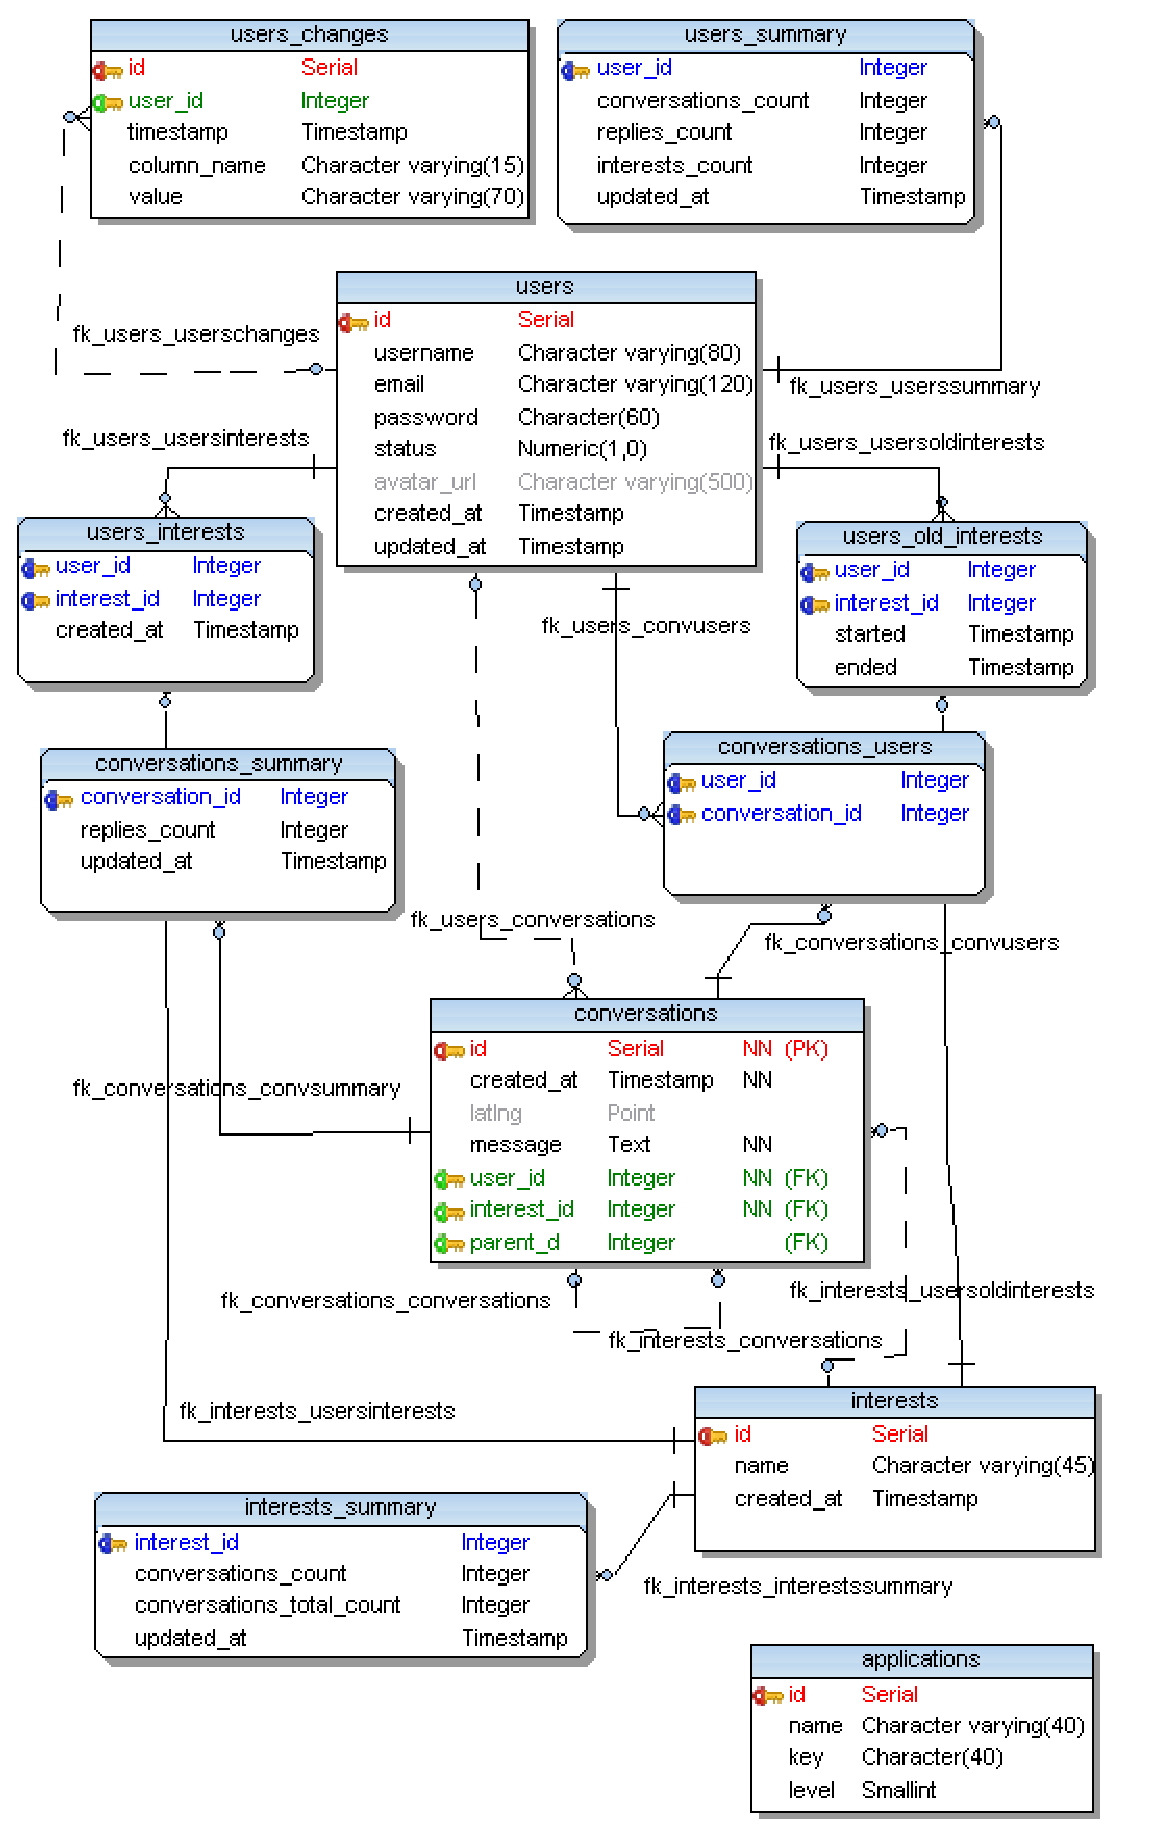
\includegraphics[height=680px]{img/er-model.eps}
		}
	}
    
    \caption{Modelo ER da aplicação.}
    \label{fig:er-model}
\end{figure}


\section{Implantação}
A implantação (também conhecida como \emph{deploy}) da API foi feita através da computação nas nuvens, devido principalmente a facilidade de alocação de recursos de acordo com a demanda, bem como custos seguindo o modelo \emph{pay-as-you-go} (pague pelo o que usar).

A vantagem de possuir capacidade de computação disponível a medida do necessário remove a necessidade de planejamento com relação a aquisição de infraestrutura, sem contar na mão de obra necessária para manutenção desta infraestrutura.

Exemplos como o do Instagram, descrito na seção \ref{subsec:stackinstagram}, mostram como é possível ter um serviço nas nuvens escalando para milhões de usuários, e em um período de tempo inferior a um ano.

Outra decisão também muito importante na implantação foi qual tipo de serviço utilizar: PaaS ou IaaS. O primeiro permite a implantação de aplicações sem a necessidade de instalação e configuração de softwares, ao custo da perda de flexibilidade até certo ponto. Enquanto que com serviços de IaaS as possibilidades se equiparam as de possuir uma infraestrutura própria, permitindo até mesmo a escolha do sistema operacional que será utilizado e a capacidade das máquinas alocadas (memória, processadores, armazenamento).

Devido à alguns dos requisitos de software existentes na API desenvolvida, como banco de dados e bibliotecas,  utilizou-se um serviço de IaaS, mais especificamente a \emph{Amazon Web Services}.

\begin{figure}[!h]
	\figurebox{380px}{img/infra.eps}
    \caption{Esquema da infraestrutura utilizando os serviços da Amazon AWS.}
    \label{fig:infra}
\end{figure}

A Figura \ref{fig:infra} ilustra como está organizada a infraestrutura do serviço na Amazon AWS. A API é executada em uma instância EC2 (tipo Micro, com Ubuntu Server 12.04 LTS 64 bit) através do servidor de aplicações uWSGI que utiliza a interface WSGI para se comunicar com a framework Flask.

Na frente do servidor está o servidor HTTP nginx, que funciona como um proxy reverso, redirencionando as requisições pertinentes ao servidor de aplicações, no caso, todas as requisições destinadas ao sub-domínio \emph{api.boardhood.com}. Enquanto que requisições ao domínio \emph{boardhood.com}, também servidas pelo nginx, são direcionadas para a página de apresentação da aplicação, composta apenas de arquivos estáticos (HTML, CSS e JS).

A instância que contém a API também comporta o banco de dados PostgreSQL 9.1 e o memcached. Uma outra instância EC2 é utilizada para monitorar a instância com a API através do software de monitoramente em rede Munin. Nesta instância também está instalado o servidor HTTP Apache, que permite o acesso aos relatórios gerados pelo Munin, como relatórios de I/O do disco rígido, utilização de armazenamento, utilização do processador, processos em execução, requisições HTTP, conexões com o PostgreSQL, além de vários outros relatórios que podem ser configurados através de plugins.

Além do EC2, a API faz uso do Amazon S3 para armazenamento dos avatares (imagens de perfil) dos usuários que são acessados pelo cliente móvel diretamente, sem passarem pelo servidor da API, sendo que esta apenas recebe a imagem (quando o usuário decide adicionar um avatar ao seu perfil), redimensiona ela (apesar de isto já ser feito no cliente, para reduzir o tempo de transferência dos dados) e a envia para o S3, salvando no banco de dados a url criada.

Tendo definido onde será implantada a API, é preciso estabelecer uma estratégia para executar a implatanção do código desenvolvido, testado e pronto para entrar em produção ou ser testado em um ambiente de \emph{staging}.

Para alcançar tal objetivo foram definidas na verdade duas estratégias, ambas tem como objetivo garantir a rápida implantação de aplicações. A primeira estratégia foi utilizada durante o desenvolvimento, com uma instância EC2 específica para testes. Nesta instância existem dois repositórios Git, um deles é um repositório \emph{bare}, que serve como um repositório remoto que recebe modificações. O outro repositório é o repositório que contém o código que será executado no servidor, e ele é atualizado automaticamente toda vez que modificações são enviadas para o repositório bare.

Em uma máquina local, utilizada para desenvolvimento, existe um repositório clone do repositório \emph{bare}, e qualquer modificação nele feita pode ser commitada e "empurrada" (\emph{push}) para o repositório \emph{bare}, que por sua vez irá, através de um script, atualizar o repositório que irá executar a aplicação.

A vantagem desta estratégia é de que ela permite que modificações sejam rapidamente implantadas e visualizadas no servidor. Entretanto, esta não é uma estratégia ideal para o ambiente de produção que, apesar de requerer um método rápido para implantação de aplicações, também requer um método que garanta que a aplicação irá funcionar, se certificando, por exemplo, de que o ambiente onde a aplicação foi implantada atende a todos os seus requisitos.

Em Python, assim como em muitas outras linguagens, muitas bibliotecas são utilizadas em aplicações e a atualização de uma delas pode significar problemas, seja pela mudança da API, modificação no comportamento de alguma função ou algum erro introduzido. De qualquer forma, uma aplicação, antes de ser implantada, precisa ser testada e é preciso garantir que as versões das bibliotecas no ambiente de produção sejam as mesmas das do ambiente de desenvolvimento.

Para se fazer isso em Python é possível fazer uso do \emph{distribute}, uma ferramenta que empacota aplicações Python e garante que durante a instalação todas as dependências da aplicação serão instaladas de acordo com as versões especificadas no pacote de instalação.

Resolvido o problema das dependências da aplicação, resta ainda definir uma forma para enviar a aplicação para o servidor, instalá-la, efetuar possíveis modificações nos arquivos de configuração dos servidores de aplicação e HTTP e reiniciá-los para que as modificações tenham efeito. Mesmo possuindo apenas um servidor para instalar a aplicação, são muitos passos a serem seguidos, e cada um deles pode abrir brechas para a inserção de erros, caso sejam executados manualmente.

Além disso, executar manualmente a implantação significa que todo o processo está armazenado apenas na cabeça de um ou alguns indivíduos, e mesmo que haja alguma documentação, sempre existe a chance de ela não estar atualizada. Para evitar este problema, uma solução muito utilizada é a criação de scripts que executam todas as etapas da implantação, servindo ainda como uma documentação sempre atualizada do processo.

Para acessar as instâncias EC2 é possível fazer uso de SSH, e pensando nisto foi criada uma ferramenta em Python chamada de Fabric. Ela permite a execução de comandos via SSH tanto em máquina local como em máquinas remotas. Com o uso desta ferramenta foram criados duas rotinas principais: uma para a instalação dos softwares básicos, como banco de dados, servidores de aplicação e HTTP, memcached, além de várias bibliotecas das quais outros softwares dependem; e outro para empacotar a aplicação e implantá-la no ou nos servidores de produção, modificando ainda arquivos de configuração necessários e reiniciando os servidores.

Com estes scripts, criar uma nova instância e implantar a aplicação é uma questão de executar uma única linha de comando, algo muito bom, se comparado com a execução manual de tais processos, algo trabalhoso e que pode levar a muitos erros durante o caminho.

\section{Aplicação Móvel}
No desenvolvimento deste serviço algumas perguntas foram levantadas desde o começo. A primeira era se seria melhor desenvolver primeiro para a Web Desktop ou para dispositivos móveis. E levando em conta os dados colocados na seção \ref{sec:computacaomovel}, ficou evidente que as possibilidades proporcionadas pelos dispositivos móveis é muito grande, sem contar que aplicações pensadas primeiro para dispositivos móveis tendem a ser mais simples e mais focadas no objetivo principal da aplicação, removendo qualquer outra funcionalidade secundária e que só teria espaço em computadores desktop.

Decidido o segmento de dispositivos a ser suportado, a segunda decisão foi a de desenvolver uma aplicação nativa ou web móvel. Depois de avaliar as possibilidades disponíveis em ambas as opções, ficou claro que apesar de a web móvel se mostrar atrativa, através da promessa de desenvolver aplicações com suporte a várias plataformas, o estado atual destas tecnologias ainda não oferecem a melhor experiência possível para usuários de dispositivos móveis, sendo que por enquanto, aplicações nativas ainda são a melhor opção.

Com a decisão de desenvolver uma aplicação nativa, restou a escolha de para qual plataforma desenvolver o aplicativo. De antemão, as plataformas do Symbian, Blackberry e Windows Phone foram descartadas, sendo as duas primeiras devido a drástica queda de popularidade e a terceira devido ao ainda pequeno número de usuários, algo que pode mudar no futuro, mas por enquanto não é interessante para um serviço que precisa do máximo de usuários possíveis.

Sendo assim, restaram as plataformas Android e iOS. Se a decisão fosse tomada levando em conta o que outros serviços da web fizeram, como Twitter, Facebook, Foursquare, Path e Instagram, iOS seria a escolha certa. Entretanto, outros fatores precisam ser levados em conta na escolha da plataforma mais adequada.

Para este serviço, a plataforma Android foi escolhida. Primeiro, porque ela já se posiciona em primeiro lugar no número de dispositivos em todo o mundo e continua crescendo. Segundo, aplicações Android são desenvolvidas na linguagem de programação Java, o que torna a curva de aprendizado menor, ao contrário do iOS, que faz uso de Objective-C. Além disso, as ferramentas de desenvolvimento para o Android podem ser executadas nos principais sistemas operacionais no mercado, ao contrário do iOS, que exige um computador Mac e, obviamente, sistema operacional Mac OS X.

A aplicação foi desenvolvida utilizando a IDE Eclipse em conjunto com o plugin ADT (\emph{Android Development Tools}), tendo como alvo dispositivos com a versão 2.1 ou superior do sistema operacional, garantindo assim que mais de 97\% dos dispositivos do mercado possam executar a aplicação.

Antes do início do desenvolvimento da aplicação, foram criados os \emph{mock-ups} (Figura \ref{fig:mockup}) da aplicação, ilustrando o posicionamento dos componentes na tela e definindo algumas convenções que seriam utilizadas por toda a aplicação, garantindo assim consistência a interface de usuário.

\begin{figure}[!h]
	\figurebox{450px}{img/mockup.eps}
    
    \caption{Primeiros mockups do aplicativo.}
    \label{fig:mockup}
\end{figure}

A medida em que as telas do aplicativo, bem como o fluxo das atividades que os usuários poderiam seguir foram definidas, a interface do usuário começou a ser criada no Photoshop, esta agora representando como a aplicação deveria ser, exatamente. Alguns podem argumentar sobre as vantagens de se criar uma UI fiél ao que se deseja no Photoshop ao invés de fazer isso diretamente na programação, algo que também é muito discutido com relação a aplicações Web. Mas a verdade é que, apesar de tudo, o Photoshop ainda dá uma liberdade maior na criação de interfaces, pois as modificações podem ser visualizadas instantaneamente, enquanto que no Android é preciso modificar o código-fonte, compilar e executar a aplicação.

\begin{figure}[!h]
	\figurebox{280px}{img/mobile-feed.eps}
    \caption{Tela principal da aplicação, exibe as conversas mais populares entre os interesses seguidos pelo usuário.}
    \label{fig:mobile-feed}
\end{figure}

Mas nem tudo dentro de uma aplicação móvel está relacionada com uma interface gráfica. Por exemplo, a comunicação entre o aplicativo e o \emph{web service} não depende de uma interface, e neste caso nem mesmo das APIs do Android. Aproveitando esta oportunidade, o desenvolvimento do aplicativo foi separado do desenvolvimento do cliente que iria se comunicar com o \emph{web service}, permitindo que este possa ser reutilizado por outras aplicações Java, se algum dia surgir esta necessidade.

\begin{figure}[!h]
	\figurebox{280px}{img/mobile-conversation.eps}
    \caption{Tela de uma conversa e suas respectivas respostas.}
    \label{fig:mobile-conversation}
\end{figure}

Este cliente fica então responsável pela comunicação através do protocolo HTTP com o \emph{web service}, sendo responsável ainda pela compressão/descompressão (normalmente gzip) de mensagens, serialização de parâmetros, autenticação e renovação de tokens de acesso. Para os usuários deste cliente é apresentada uma única interface de acesso, contendo todos os métodos disponíveis no \emph{web service}. Tanto os argumentos destes métodos como as respostas dadas são instâncias de classes definidas pelo cliente, que representam as entidades do serviço, que são: usuários, conversas e interesses.

A aplicação Android, portanto, apenas importa o cliente do \emph{web service}. Por se tratar de um cliente que precisa fazer acessos a rede para se comunicar com o \emph{web service}, tarefa custosa em aplicações móveis, o aplicativo faz uso do cliente através de tarefas assíncronas (executadas em segundo plano, em \emph{threads} separadas). Isso significa que enquanto o aplicativo estiver se comunicando com o \emph{web service}, a interface de usuário não será bloqueada, algo que definitivamente não ajuda na experiência do usuário.

\begin{figure}[!h]
	\figurebox{420px}{img/mobile-profile.eps}
    
    \caption{Perfil de um usuário, exibindo as suas conversas mais recentes.}
    \label{fig:mobile-profile}
\end{figure}

A tela principal da aplicação é a tela de \emph{Feeds} (Figura \ref{fig:mobile-feed}). Nela são exibidas as conversas mais populares, de acordo com o algoritmo explicado na seção \ref{subsec:algopopularidade}, dentro dos interesses do usuário e, opcionalmente, filtradas de acordo com a localização. Através dos filtros disponíveis é possível escolher a forma como estas conversas poderão ser ordenadas, que pode ser, além da popularidade, a distância com relação a localização do usuário ou a data de criação da conversa.

No aplicativo, todas as listas seguem o mesmo padrão para a atualização e paginação. A primeira é feita através do botão mais a direita na action bar, clicando nele o aplicativo verifica no \emph{web service} se novas conversas surgiram após a última atualização da lista. Já a paginação é feita através de um botão que fica posicionado ao fim lista, e quando o usuário clica no botão o aplicativo carrega um determinado número de conversas.

\begin{figure}[!h]
	\figurebox{280px}{img/mobile-explore.eps}
    \caption{Tela de busca de interesses.}
    \label{fig:mobile-explore}
\end{figure}

Existem, entretanto, outras maneiras de se abordar estas duas funcionalidades. A atualização de listas, por instância, pode ser feita através do mecanismo conhecido como \emph{pull-to-refresh}, que é patenteado pelo Twitter. As atualizações também podem ser automáticas, com o uso de um servidor \emph{push} que envia as atualizações para o smartphone quando elas ocorrerem. Já a paginação pode ser feita através da lista infinita, que carrega a próxima página toda a vez que o usuário atingir o final da lista.

\begin{figure}[!h]
	\figurebox{280px}{img/mobile-interest.eps}
    \caption{Tela do interesse sobre Fotografia.}
    \label{fig:mobile-interest}
\end{figure}

As conversas exibidas no \emph{Feed} são apenas as conversas iniciadas por usuários, ou seja, respostas de outros usuários não aparecerão nesta listagem. Cada item da lista contém o nome e avatar do usuário que criou a conversa, o interesse onde esta conversa foi criada, o conteúdo da conversa, a quanto tempo ela foi criada, quantas respostas ela já obteve e a que distância do usuário do aplicativo ela foi criada, esta última implicando que tanto o usuário do aplicativo como o criador da conversa permitiram que sua localização fosse utilizada.

Ao pressionar um dos itens da lista, o usuário irá visualizar a conversa em conjunto com as respostas dadas a ela, como mostra a Figura \ref{fig:mobile-conversation}. Acima da conversa inicial está a identificação do interesse ao qual a conversa pertence que, ao ser pressionado levará o cliente a tela do interesse. Tanto nesta tela como na de \emph{Feeds}, ao pressionar o avatar de um usuário, o perfil do mesmo será exibido.

Nesta tela também existe o botão para atualizar as conversas, mas ao contrário da tela de \emph{Feeds}, aqui as novas conversas são posicionadas ao final da lista, levando em conta que esta está em ordem cronológica.

Como fora dito anteriormente, ao clicar no avatar de um usuário, o seu perfil será exibido na tela. Agora, não existem informações, além de seu nome de usuário, a serem exibidas. Deste modo, grande parte da tela é utilizada para a exibição das conversas criadas pelo usuário, bem como respostas a outras conversas e os interesses que este usuário segue. A separação entre a visualização das conversas mais recentes de um usuário e os interesses que ele segue é feita através de abas. Na Figura \ref{fig:mobile-profile} é possível ver a esquerda a aba de conversas e a direita a aba de interesses do usuário.

Para que um usuário possa ter seu \emph{feed} de conversas ele precisa seguir interesses, e para tanto, é preciso haver um meio de se pesquisar os interesses existentes, para então começar a seguí-los. A tela \emph{Explore} serve exatamente para este propósito, permitindo que usuários busquem interesses ou mesmo criem novos interesses, caso não eles não existam. Na Figura \ref{fig:mobile-explore} é possível visualizar esta tela. Seu funcionamento é simples, basta ao usuário começar a digitar as letras do interesse desejado e a lista será atualizada, exibindo interesses que contenham o mesmo prefixo.

Seja através da tela de \emph{Explore} ou através de conversas, um usuário pode ir para a tela de um interesse, podendo desta forma visualizar quais são os usuários que seguem o interesse e quais as últimas conversas criadas nele, como é mostrado na Figura \ref{fig:mobile-interest}.

\begin{figure}[!h]
	\figurebox{280px}{img/mobile-new-conversation.eps}
    \caption{Tela para criação de nova conversa.}
    \label{fig:mobile-new-conversation}
\end{figure}

Por fim, a funcionalidade central da aplicação, que é a criação de uma nova conversa, esta tela vista na Figura \ref{fig:mobile-new-conversation}. Esta tela atua, na verdade, como um diálogo, ficando sobre a tela atual que o usuário estava visualizando. Esta funcionalidade é acionada através do botão central da \emph{footer bar} do aplicativo, e ela pode utilizar informações da tela atual para preencher as informações para criação da nova conversa.

Por exemplo, se o usuário estiver na tela do interesse Fotografia, quando ele pressionar o botão para criação de uma nova conversa, o aplicativo irá assumir que a nova conversa será colocada no interesse Fotografia, muito embora o usuário possa alterar o interesse posterirmente. Da mesma forma, se o usuário estiver visualizando uma conversa, quando ele for criar uma nova conversa, presume-se que esta será uma resposta a conversa visualizada.

Através de tais padrões de comportamento implícitos, é possível facilitar a vida do usuário. Entretanto, uma vez que o usuário tenha pressionado o botão para criar a conversa, é necessário trazer a tona este comportamento, mostrando que a conversa que ele está criando será colocada em determinado interesse ou será uma resposta a determinada conversa, tornado assim explícito o comportamente, e removendo qualquer dúvida sobre o funcionamento do aplicativo.


\section{Unindo as partes}
Talvez uma das tarefas mais difíceis e ao mesmo tempo mais empolgante no desenvolvimento de uma aplicação seja colocar ela para funcionar e ver todas as partes se conversando entre si. E não se trata apenas dos componentes de um software, mas de todo o serviço, incluindo aqui os testes, a documentação da aplicação, os scripts utilizados na implantação, e as ferramentas de monitoramento.

Tudo precisa ser pensando de forma a facilitar a evolução deste serviço, garantindo, em primeiro lugar, a qualidade na experiência dos usuários.

E isso se traduz em cada uma das etapas do desenvolvimento do serviço. Seja na utilização de testes unitários e de integração, para garantir que a aplicação está se comportando conforme o experado, seja na criação de processos para implantação da aplicação que garantam consistência, segurança e rapidez. Ou no cuidado com o qual a interface gráfica da aplicação foi criada, que, acima de tudo, transmite aos usuários o nível de comprometimento do serviço com a qualidade.

Nem sempre é possível fazer algo da forma certa na primeira vez, em muitos dos casos pois o que é certo ou não não está claro o suficiente. Mas se há algo que a Internet possibilitou foi a troca de experiências, que é algo de valor inestimável, mas muitas vezes ignorado.

Durante cada uma das etapas de desenvolvimento deste seviço sempre buscou-se encontrar relatos de outras pessoas e empresas, com o intuito de antecipar ou evitar problemas, e elencar estratégias para curto e longo prazo.

Com este relatório espera-se que outras pessoas possam tirar vantagem das experiências aqui documentadas.


% Conclusão
%%%%%%%%%%%%%%%%%%%%%%%%%%%%%%%%%%%%%%%%%%%%%%%%%%%%%%%%%%%%%%%%%%%%%%%%%%%%%%%%
\chapter*{Conclusão}
Conceber um serviço, desde suas características básicas até a sua implatanção é uma tarefa que requer tempo e dedicação. Ela também envolve muitas questões que precisam ser levantadas e estudadas para que então possa-se definir as opções disponíveis, qual é a mais adequada e que impacto isso terá no serviço como um todo.

Cada decisão tomada precisa levar em conta o objetivo principal do trabalho, que é colocar o serviço em funcionamento, atrair usuários, receber \emph{feedback} dos mesmos, melhorar o serviço e iterar.

Ao refletir sobre o formato atual dos fóruns e como eles poderiam ser melhorados, buscando ideais provenientes das redes sociais, este trabalho conseguiu criar um serviço que mantém a essência dos fóruns, permitindo a criação de comunidades online, mas que ao mesmo tempo atende as expectativas que muitos usuários podem vir a ter quanto a um serviço da Internet nos dias de hoje, comprovando desta forma a primeira das hipóteses deste trabalho.

Neste mesmo sentido, a escolha da estratégia de criar a aplicação móvel primeiro também foi acertada. Primeiro porque o mercado móvel está crescendo em ritmo constante, com cada vez mais pessoas tendo acesso a Internet através de \emph{smartphones}. E segundo, porque a construção de uma aplicação móvel impôs muitas restrições com relação as funcionalidades dos serviços, obrigando a remoção de características supérfluas e dando foco as funcionalidades realmente importantes.

E uma destas funcionalidades foi a geolocalização. O uso dela neste serviço não se tratou apenas de seguir uma tendência, da qual ela de fato faz parte, mas sim de melhorar a experiência dos usuários. Através dela um indivíduo pode se engajar em discussões sobre assuntos que lhe interessam, e fazê-lo com pessoas que estão próximas dele, possibilitando a criação de comunidades que, além de compartilharem interesses em comum, também façam parte de uma mesma localização geográfica.

Apesar disto, a hipótese de que a geolocalização por si cria um diferencial com relação as outras redes sociais não pôde ser comprovada. Isso porque este serviço serve a um propósito diferente do das redes sociais, e nele a geolocalização tem o papel de permitir que indivíduos participem de discussões com pessoas que estão próximas dele. Além disso, as principais redes sociais já fazem uso da geolocalização de alguma forma.

O uso da geolocalização também proporcionou a experimentação de diversos bancos de dados, em uma busca pelo mais adequado para o serviço em vista. Esta decisão, de caráter técnico, foi tomada através de testes que demonstrarão qual a melhor opção disponível, levando em conta ainda características inerentes a cada um dos bancos de dados.

Outra decisão técnica foi a autenticação da API RESTful. E infelizmente, a terceira das hipóteses não pode ser comprovada, pois a implementação do protocolo OAuth requer tempo e um projeto maduro. Entretanto, a implementação utilizada neste serviço atendeu as necessidades atuais sem, entretanto, exceder o cronograma do trabalho.

Através do estudo aprofundado das áreas que seriam utilizadas na criação deste serviço, bem como a tomada de decisões levando em conta não somente questões técnicas, mas também as características e restrições do trabalho, os recursos disponíveis e, principalmente, a experiência do usuário como um todo, este trabalho foi capaz de criar um serviço em sua completude.


% Trabalhos Futuros
%%%%%%%%%%%%%%%%%%%%%%%%%%%%%%%%%%%%%%%%%%%%%%%%%%%%%%%%%%%%%%%%%%%%%%%%%%%%%%%%
\chapter*{Trabalhos Futuros}
Neste trabalho foram documentadas todas as etapas do desenvolvimento de uma aplicação móvel até o momento de sua implantação. Entretanto, a partir do momento em que o serviço está no ar existem outras questões que ao longo do tempo precisarão ser respondidas.

Uma delas diz respeito a possibilidade de o serviço crescer e consequentemente da necessidade de comportar este crescimento. A escalabilidade, bem como algumas estratégias para se obtê-la em vários dos componentes que fazem parte de uma aplicação foram abordados neste trabalho sem, entretanto, um aprofundamento nos assuntos.

Uma das propostas para trabalhos futuros seria o estudo de arquiteturas, tecnologias e estratégias para se escalar aplicações web, abordando questões como distribuição da aplicação em vários servidores, balanceadores de carga, redes de distribuição de conteúdo, sistemas de cache de dados, e replicação e sharding de bancos de dados.

Já partindo mais para o lado conceitual do serviço, seria possível desenvolver uma análise sobre o estado atual do serviço, se ele deu certo ou não e quais foram as razões, bem como um levantamento do que poderia melhorar no serviço e quais seriam os próximos passos na evolução do mesmo, buscando fomentar a criação de discussões e o crescimento das comunidades dentro do serviço.

Com relação a criação de comunidades e discussões, seria interessante analisar o comportamento dos usuários dentro do serviço, em que contextos as discussões ocorrem, e qual o perfil da maioria dos usuários. E partindo para o lado mais técnico, seria possível avaliar a quantidade de spam gerado no serviço, bem como a qualidade do mesmo, dando sugestões para a redução do primeiro e aumento do segundo.

E é importante lembrar que os fóruns já introduziram alguns mecanismos para evitar spams e elevar a qualidade nas discussões, se utilizando, por exemplo, de moderadores. Entretanto, o uso de moderadores nem sempre é uma estratégia escalável, tornando interessante o estudo de alternativas para a remoção de spams, bloqueio de usuários problemáticos (trolls) e remoção de conversas inapropriadas.

A verdade é que um serviço com a natureza como a deste possuí muitos desafios pela frente que precisarão ser, uma hora ou outra, enfrentados, sejam eles de natureza tecnológica ou comportamental.


\bibliographystyle{template/abnt}
\bibliography{bibliography}

\end{document}